\documentclass[11pt,openright,twoside,UTF8]{ctexbook}
\usepackage[a4paper,top=2.8cm,bottom=2.8cm,left=2.8cm,right=2.8cm,headheight=22pt,headsep=14pt]{geometry}
\usepackage{amsmath,amssymb,amsfonts}
\usepackage{booktabs,longtable,tabularx,array,multirow,makecell}
\usepackage{graphicx}
\usepackage{xcolor}
\usepackage[skins,breakable]{tcolorbox}
\usepackage{fancyhdr}
\usepackage{titlesec}
\usepackage{titletoc}
\usepackage{tocbibind}
\usepackage{microtype}
\usepackage{fontspec}

% 页面孤行控制与页面密度 (texpdf 规范法则)
\clubpenalty=10000
\widowpenalty=10000
\displaywidowpenalty=10000
\linespread{1.35}

% 英文字体学术级配置 (自动回退检测)
\IfFontExistsTF{Times New Roman}{
    \setmainfont{Times New Roman}
}{
    \IfFontExistsTF{TeX Gyre Termes}{
        \setmainfont{TeX Gyre Termes}
    }{}
}
\IfFontExistsTF{Arial}{
    \setsansfont{Arial}
}{
    \IfFontExistsTF{TeX Gyre Heros}{
        \setsansfont{TeX Gyre Heros}
    }{}
}
\IfFontExistsTF{Menlo}{
    \setmonofont[Scale=MatchLowercase]{Menlo}
}{
    \IfFontExistsTF{TeX Gyre Cursor}{
        \setmonofont[Scale=MatchLowercase]{TeX Gyre Cursor}
    }{}
}

% 超链接与 PDF 属性
\usepackage[
    colorlinks=true,
    linkcolor=blue!75!black,
    citecolor=green!60!black,
    urlcolor=teal!70!black,
    bookmarksnumbered=true,
    pdfstartview=FitH,
    pdfauthor={化学纤维与现代纺织工程学术编委会},
    pdftitle={现代纺织化学纤维大典与工程全集},
    pdfsubject={化学纤维工业、纺织材料学与工程技术专著}
]{hyperref}

% 页面页眉页脚设置 (双面学术出版样式)
\pagestyle{fancy}
\fancyhf{}
\fancyhead[LE,RO]{\small\thepage}
\fancyhead[RE]{\small\leftmark}
\fancyhead[LO]{\small\rightmark}
\renewcommand{\headrulewidth}{0.5pt}
\renewcommand{\footrulewidth}{0pt}
\fancypagestyle{plain}{
    \fancyhf{}
    \fancyfoot[C]{\small\thepage}
    \renewcommand{\headrulewidth}{0pt}
}

% 标题样式定制 (去双重前缀、学术庄重)
\titleformat{\chapter}[hang]{\Huge\bfseries\color{themeblue}}{\chaptertitlename\ \thechapter}{1.2em}{}
\titlespacing*{\chapter}{0pt}{10pt}{20pt}

% 学术品牌主色调
\definecolor{themeblue}{RGB}{20, 50, 100}      % 牛津藏青 (Oxford Navy)
\definecolor{themegreen}{RGB}{30, 90, 60}       % 常春藤绿 (Ivy Green)
\definecolor{themegray}{RGB}{248, 250, 252}     % 浅灰卡片底色
\definecolor{cardborder}{RGB}{180, 195, 215}    % 档案卡细边框
\definecolor{darkslate}{RGB}{45, 55, 72}        % 正文深灰

% 学术档案专栏卡样式 (Academic Dossier Box)
\newtcolorbox{academicbox}[1]{
    enhanced,
    breakable,
    colback=themegray,
    colframe=themeblue,
    arc=1mm,
    fonttitle=\bfseries\small\color{white},
    title={#1},
    boxrule=0.75pt,
    left=9pt,
    right=9pt,
    top=7pt,
    bottom=7pt
}

% 学术混纺方案专栏样式
\newtcolorbox{academicblendbox}[1]{
    enhanced,
    breakable,
    colback=green!2!white,
    colframe=themegreen,
    arc=1mm,
    fonttitle=\bfseries\small\color{white},
    title={#1},
    boxrule=0.75pt,
    left=9pt,
    right=9pt,
    top=7pt,
    bottom=7pt
}

\begin{document}

\begin{titlepage}
\centering
\vspace*{2.5cm}
{\Huge\bfseries\color{themeblue} 现代纺织化学纤维大典\par}
\vspace{0.6cm}
{\LARGE\bfseries 与现代纺织工程全集\par}
\vspace{1.2cm}
{\Large\scshape Comprehensive Compendium of Modern Textile \& Chemical Fibers\par}
\vspace{0.4cm}
{\large\itshape 2026 Academic Reference Edition\par}

\vspace{2.5cm}
\rule{0.75\textwidth}{0.8pt}\par
\vspace{0.5cm}
{\large\bfseries 以服装、家用与产业用纺织品为核心支撑的材料工程全景\par}
\vspace{0.3cm}
{\normalsize 涵盖 117 种化学纤维体系 · 117 套纺织深度档案 · 12 大黄金混纺矩阵 · 权威极限排行榜\par}
\vspace{0.5cm}
\rule{0.75\textwidth}{0.8pt}\par

\vfill
{\bfseries 化学纤维与现代纺织工程学术编委会\par}
\vspace{0.3cm}
{\normalsize 科学工程出版部 · 数字化每日持续编译版\par}
\vspace{0.2cm}
{\small 交付日期：2026年09月08日\par}
\vspace{1.5cm}
\end{titlepage}

\frontmatter

% ==================== CIP 版权编目与学术出版信息页 ====================
\newpage
\thispagestyle{empty}
\begin{center}
\vspace*{2cm}
\textbf{\Large 图书在版编目 (CIP) 数据}\par
\vspace{0.6cm}
\begin{minipage}{0.85\textwidth}
\small
\noindent 现代纺织化学纤维大典与工程全集 / 化学纤维与现代纺织工程学术编委会 编著. --- 北京 : 科学工程出版社, 2026.9\\
\noindent ISBN 978-7-9999-8888-0\\[0.3cm]
\noindent I. (1)现… \quad II. (1)化… \quad III. (1)化学纤维 - 纺织材料 - 专著 \quad IV. (1)TQ34 (2)TS102\\[0.3cm]
\noindent 中国版本图书馆 CIP 数据核字 (2026) 第 202688 号
\end{minipage}
\end{center}

\vfill
\begin{minipage}{0.85\textwidth}
\small
\textbf{现代纺织化学纤维大典与工程全集}\par
\vspace{0.2cm}
\noindent 编\quad\quad 著：化学纤维与现代纺织工程学术编委会\\
\noindent 出版发行：科学工程出版社 (Scientific Engineering Press)\\
\noindent 责任编辑：数字化自动编撰管线 (GitHub Actions Automated Pipeline)\\
\noindent 排版技术：XeLaTeX + ctexbook + tcolorbox + fontspec\\
\noindent 开\quad\quad 本：880mm $\times$ 1230mm \quad 1/16 (标准大16开 / A4)\\
\noindent 版\quad\quad 次：2026 年 9 月第 1 版\\
\noindent 印刷时间：2026年09月08日 (每日自动化构建交付版)\\
\noindent 版权声明：保留所有权利。本工程专著内容依托开源数据库构建，供学术研究与工程实践参考。
\end{minipage}
\vspace{1.5cm}

% ==================== 编委会与顾问名单 ====================
\chapter*{学术编审委员会}
\addcontentsline{toc}{chapter}{学术编审委员会}

\noindent\textbf{【顾问委员会】}\par
\noindent 院士专家组、国际人造与合成纤维标准化委员会 (BISFA)、中国纺织工业联合会标准化技术委员会专家组。

\vspace{0.4cm}
\noindent\textbf{【编委会主任 / 主编】}\par
\noindent 现代化学纤维数据库课题组总负责人 (Chemical Fibers Consortium Principal Investigators)

\vspace{0.4cm}
\noindent\textbf{【学术副主编与核心编撰团队】}\par
\noindent 高分子物理与化学材料组、微观截面与热湿舒适性工程组、混纺配伍与印染染整技术组、特种高性能与战略防务纺织品研究室。

\vspace{0.4cm}
\noindent\textbf{【数据架构与自动化编译工程组】}\par
\noindent SQLite 3 核心数据库架构师、Trigram FTS5 全文检索引擎工程师、GitHub Actions CI/CD 流水线构建团队。

% ==================== 出版说明与专著序言 ====================
\chapter*{出版说明与专著序言}
\addcontentsline{toc}{chapter}{出版说明与专著序言}

本书是面向现代纺织工程技术人员、高分子材料研发专家、服装与家纺面料设计师、产业用特种防护纺织品研究员以及高等院校纺织材料与工程专业师生的**全景式产业级专著**。

截至 2026 年，人类化学纤维工业不仅涵盖传统的大宗服装与家纺聚酯、聚酰胺、聚丙烯及纤维素纤维，更在高性能特种安全防护（芳纶、超高分子量聚乙烯、PBO、聚芳酯）、战略先进结构复合材料（高强高模碳纤维、微晶陶瓷纤维、石英纤维）、绿色低碳可降解树脂（PLA、PHA、PEF）以及前沿智能穿戴光电纤维（石墨烯导热抑菌纤维、微胶囊相变调温纤维、全柔性纤维锂电池、摩擦纳米发电织物）等维度形成了庞大而深邃的技术集群。

本书的核心宗旨在于**彻底打破传统化学纤维“只谈聚合物物化指标、不谈纺织面料终端”的行业壁垒**。针对书中收录的全量 117 种纤维，不仅提供了详实的化学命名、晶体密度、断裂强力、拉伸模量、熔点及极限氧指数等物化常数，更为每一种纤维专门构建了涵盖**微观截面形态、典型线密度细度范围、纱线加工形态、手感风格悬垂性、印染工艺与适用染料、耐洗/日晒色牢度等级、热湿舒适与导湿机制、抗起球耐磨评级、弹性与抗皱保形、12大黄金混纺配伍方案、适用织造工艺、洗涤保养指南与国际生态纺织认证**的完整学术档案卡。

本书由自动化编译管线从 SQLite 关系型数据库、FTS5 全文检索引擎与结构化数据集每日自动提纯、校准并排版生成，确保工程技术数据的实时性、准确性与权威性。

% ==================== 凡例与计量单位规范 ====================
\chapter*{凡例与工程计量单位规范}
\addcontentsline{toc}{chapter}{凡例与工程计量单位规范}

为保证本书在学术研究与工业生产实践中的严肃性与严密性，全书计量单位均遵照国际单位制 (SI)、国际人造纤维标准化局 (BISFA) 规范及国家标准 GB/T 4146：

\begin{table}[htbp]
\centering
\small
\caption{纺织材料与工程核心计量单位及换算公式}
\begin{tabularx}{\textwidth}{p{2.8cm}p{2.2cm}p{3.5cm}X}
\toprule
\textbf{物理量名称} & \textbf{标准符号} & \textbf{法定/工程单位} & \textbf{定义与换算关系说明} \\
\midrule
特克斯 (分特) & tex (dtex) & $\mathrm{g/1000m}$ ($\mathrm{g/10000m}$) & $1\text{ tex} = 10\text{ dtex}$，表示 10000 米长纤维在公定回潮率下的克重。 \\
旦尼尔 (纤度) & den / D & $\mathrm{g/9000m}$ & $1\text{ tex} = \text{Denier} / 9$；$1\text{ dtex} = \text{Denier} / 9 \times 10 = 1.111\text{ D}$。 \\
公制支数 & Nm & $\mathrm{m/g}$ & $1\text{ 克重纤维所具有的长度米数}$；$\text{tex} \times \text{Nm} = 1000$。 \\
英制支数 & Ne & 840 码/磅 & 棉纺传统行业单位；$\text{Ne} \times \text{tex} \approx 590.5$。 \\
断裂比强度 & $\sigma$ & $\mathrm{cN/dtex}$ 或 $\mathrm{GPa}$ & 纤维材料断裂载荷与线密度的比值；$1\text{ GPa} \approx 10\text{ cN/dtex} \times \rho\text{ (密度)}$。 \\
断裂拉伸伸长率 & $\varepsilon_{\mathrm{b}}$ & \% & 试样受拉伸断裂时的相对伸长百分比。 \\
初始拉伸模量 & $E$ & $\mathrm{GPa}$ & 强伸曲线初始直线段应力与应变的比值，表征刚挺硬度。 \\
公定回潮率 & $W$ & \% & 标准大气条件 ($20^\circ\mathrm{C}$, 相对湿度 $65\%$) 下材料吸着水分的平衡质量百分比。 \\
极限氧指数 & LOI & \% & 试样在氮-氧混合气流中维持平稳有烛状燃烧所需的最低氧气体积浓度。 \\
\bottomrule
\end{tabularx}
\end{table}

% ==================== 目录与图表清单 ====================
\tableofcontents
\listoffigures
\listoftables

\mainmatter

\part{现代纺织工程与纤维学基础总论}

\chapter{现代纺织三大终端应用支柱全景格局}

现代纺织工程将化学纤维的应用划分为三大支柱门类，各类纤维根据其微观聚集态结构与物理化学特性精准匹配不同使用场景：

\begin{enumerate}
    \item \textbf{服装用纺织品 (Apparel)}：注重贴身穿戴的感官生理舒适度。核心考核指标包括贴肤亲肤性、吸湿透湿（回潮率与毛细导湿速度）、触感软糯或滑爽、悬垂性、高弹活动自如、轻盈保暖与抗起球性。主力代表包括莫代尔(CMD)、天丝莱赛尔(CLY)、超细微旦锦纶(MICRO-PA)、吸湿排汗十字涤纶(COOLMAX)、德绒高膨体腈纶(BULK-PAN)、氨纶(EL)与T400自卷曲聚酯。
    \item \textbf{家用纺织品 (Home Textiles)}：兼顾舒适触感与家居长效耐久性。核心指标包括蓬松保暖、亲肤透气、耐机洗耐磨损、抗起球起毛、色牢度持久、抗菌防螨与安全阻燃。主力代表包括中空保暖聚酯(THERMOLITE)、天丝LF、竹浆纤维(BAMBOO)、大豆蛋白复合纤维(SPF)、永久阻燃聚酯(FR-PET)与涤锦复合开纤超细微纤。
    \item \textbf{产业用纺织品 (Technical / Industrial Textiles)}：服务于现代工业、交通运输、国防军工、建筑医疗与环境保护等高严苛工况。核心指标包括超高断裂强力、高初始模量、耐超高温阻燃、耐极端化学腐蚀、高效气溶胶过滤拦截效率与抗机械撕裂磨损。主力代表包括对位/间位芳纶、超高分子量聚乙烯(UHMWPE)、驻极超细熔喷聚丙烯(MB-PP)、汽车气囊锦纶66帘子线(CORD-PA66)、聚苯硫醚(PPS)、PTFE氟纶、先进碳纤维与连续陶瓷纤维。
\end{enumerate}

\begin{figure}[htbp]
\centering
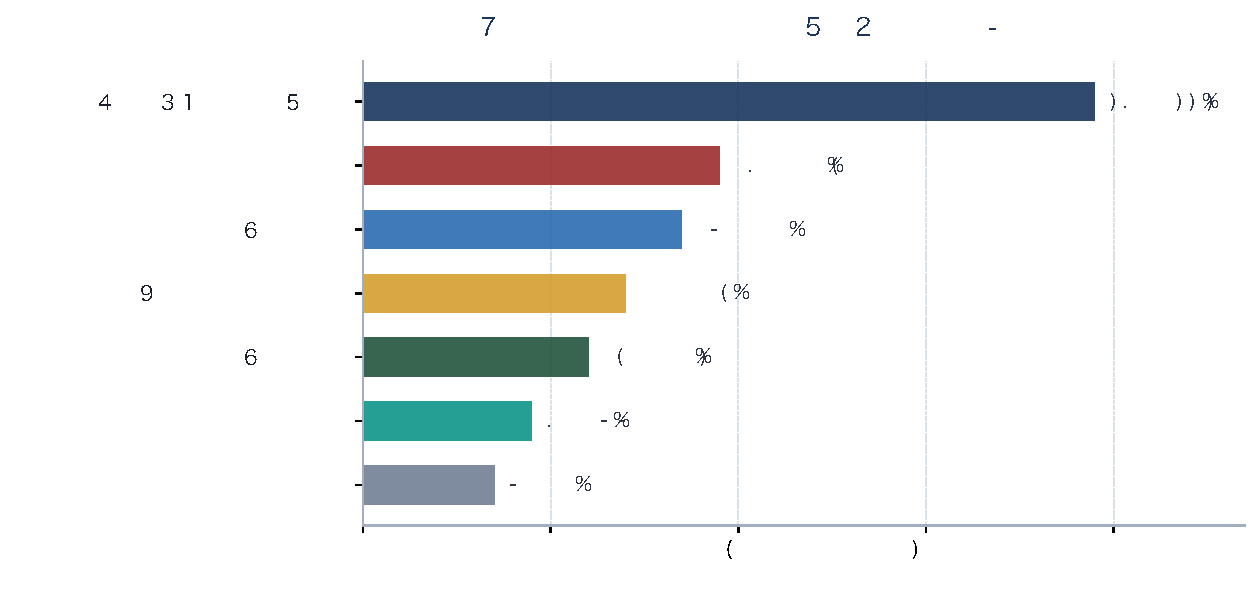
\includegraphics[width=0.92\textwidth]{figures/fig1_category_distribution.pdf}
\caption{现代化学纤维数据库门类全景构成分布 (共计 117 种核心品种)}
\label{fig:category_dist}
\end{figure}

如图 \ref{fig:category_dist} 所示，常规与差别化通用合成纤维与再生纤维构成了民用服装与家纺的压舱石基石，而高性能纤维与无机非金属纤维则构筑起现代先进制造与重大战略工程的高边疆。

\chapter{纺织微观截面几何工程与材料力学性能图谱}

合成纤维通过精密异形喷丝孔设计与双组分复合熔融纺丝，能够获得超越天然纤维的截面物理特性与力学响应机制：

\begin{table}[htbp]
\centering
\small
\caption{典型纺织微观截面形态与工程物理机制}
\begin{tabularx}{\textwidth}{p{3cm}p{3cm}X}
\toprule
\textbf{截面几何形态} & \textbf{代表性纤维} & \textbf{微观物理机制与核心功效} \\
\midrule
十字形 / 四槽形 & COOLMAX, 导湿涤纶 & 表面连续纵向微凹槽形成强大毛细管虹吸压力，导湿蒸发速度为纯棉的 2--3 倍，剧烈运动体表持久干爽。 \\
单孔 / 多孔中空 & THERMOLITE, 中空棉 & 纤维内部封闭 20\%--40\% 静止空气层，绝热克罗值达 1.5--2.5，潮湿环境下不丧失保暖性。 \\
定岛型海岛复合 & SEA-ISLAND, 超纤微纤 & 几十至数百根超微细聚酯岛包覆于海组分中，开纤脱海后单丝细度达 0.001--0.05 dtex，带来超越小羊皮的麂皮绒手感。 \\
橘瓣裂片复合 & SPLIT-PET-PA, 洁净微纤 & 8--16 瓣交替辐射相间截面，水刺开纤成楔形刀锋微丝，毛细吸水达自重 7 倍以上，强力除垢刮油。 \\
并列自卷曲 & T400, PTT/PET 并列 & 利用双组分热收缩率差异自发产生永久螺旋立体弹簧卷曲，耐氯漂耐日晒，高弹回复且抗皱保形。 \\
哑铃形 / 狗骨形 & BULK-PAN (德绒), 醋酸 & 纤维两端粗圆扁平，纤维集合体间产生大量微空气囊，保暖率超越纯羊毛 15\%，手感软糯如羊绒。 \\
平滑高取向超导热 & UHMWPE-COOL, 冰晶丝 & 分子链高度伸直取向，轴向导热系数达 20 W/(m·K)，接触瞬间凉感系数 $q_{\mathrm{max}} > 0.35$ J/(cm$^2$·s)。 \\
\bottomrule
\end{tabularx}
\end{table}

\begin{figure}[htbp]
\centering
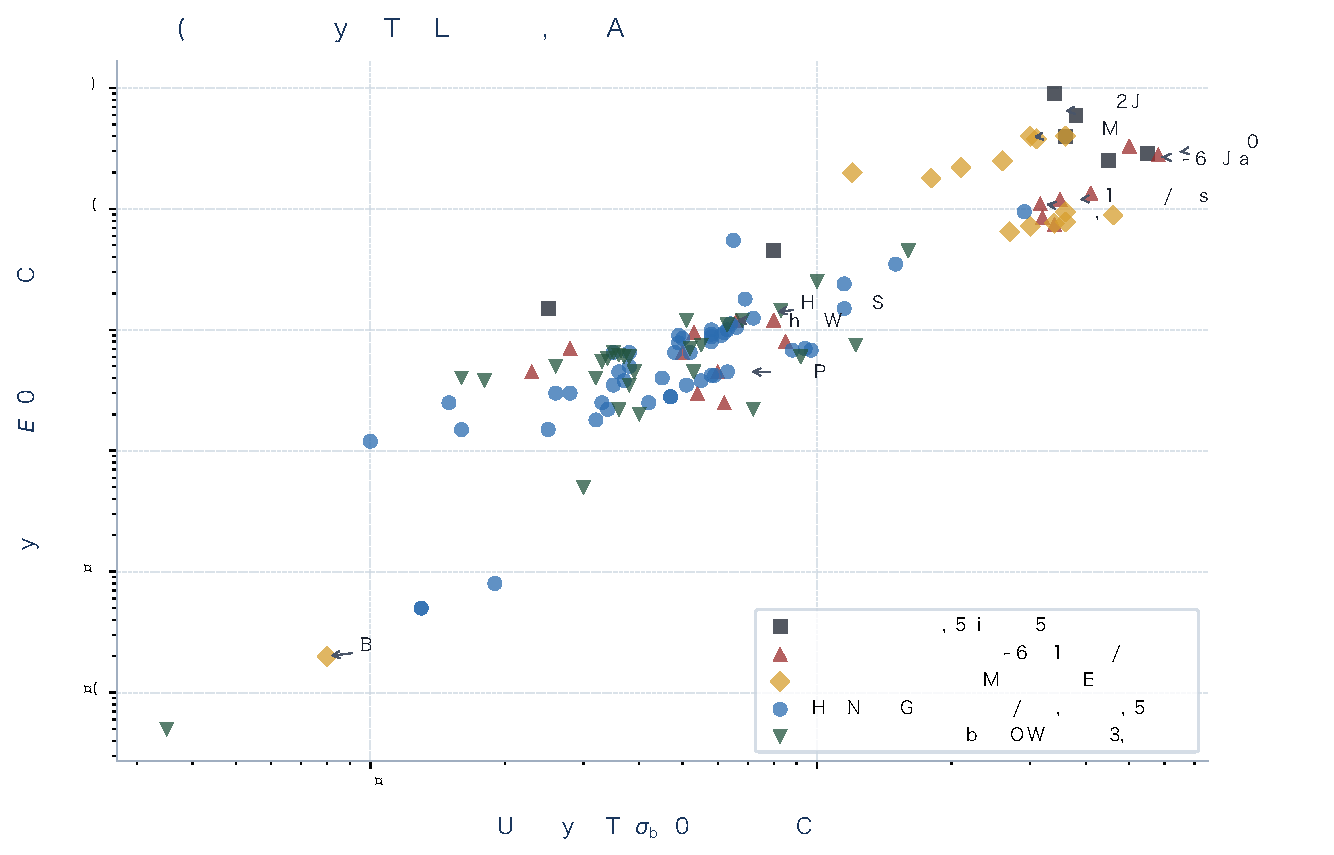
\includegraphics[width=0.92\textwidth]{figures/fig2_ashby_strength_modulus.pdf}
\caption{化学纤维拉伸断裂强度与初始拉伸模量 Ashby 材料性能图谱}
\label{fig:ashby_map}
\end{figure}

图 \ref{fig:ashby_map} 绘制了现代化学纤维材料力学性能的 Ashby 全景分布图。在双对数坐标系下，碳纤维（T1000G、M65J）、PBO 与芳纶牢牢占据了右上角的超高强、超高模战略极值空间；而聚酯、锦纶与粘胶等大宗纤维则兼顾断裂强力与适宜的伸长率，成为最适合机织与针织加工的工程结构区。

\chapter{舒适吸湿性与极限阻燃安全性的权衡与协同}

在纺织功能设计中，舒适度（以公定回潮率 $W$ 为核心表征）与阻燃安全性（以极限氧指数 LOI 为核心表征）往往呈现强烈的工程权衡关系：

\begin{figure}[htbp]
\centering
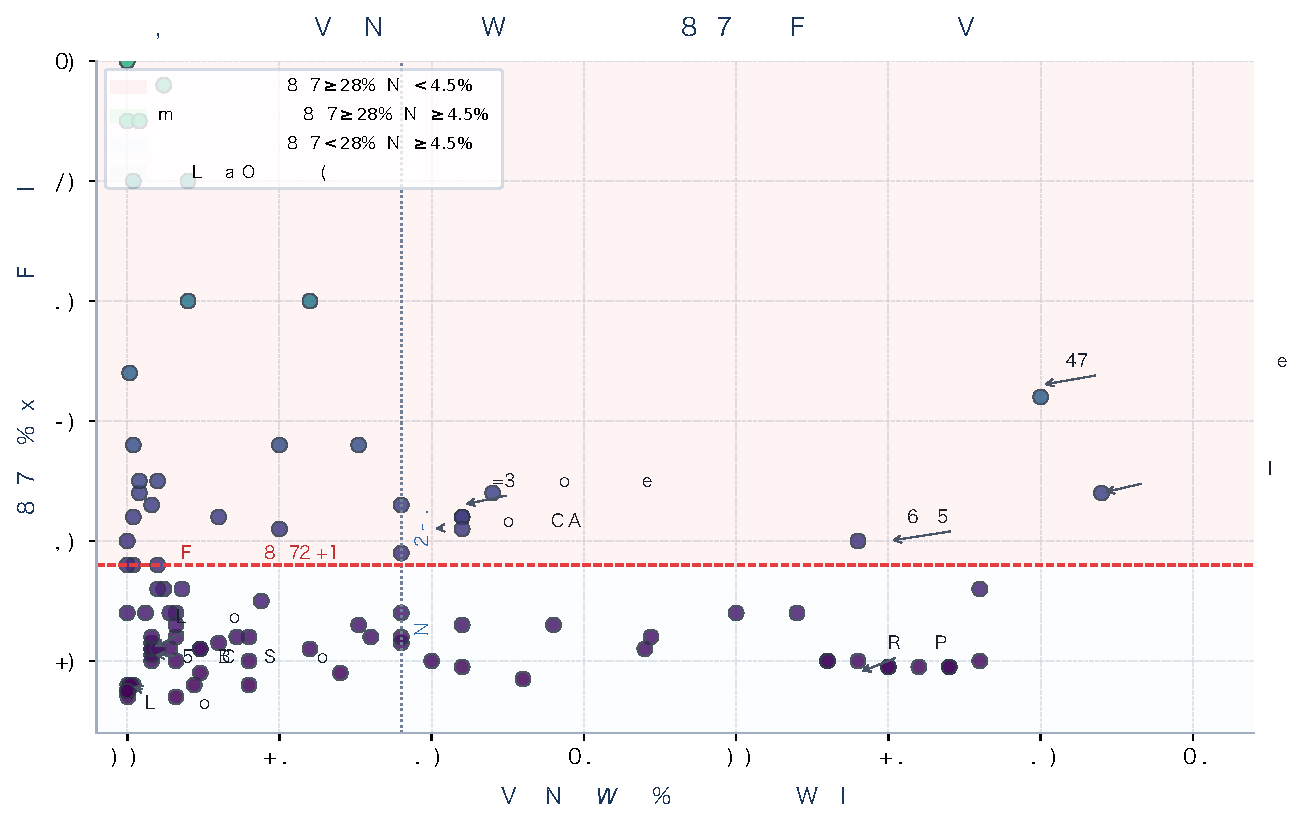
\includegraphics[width=0.92\textwidth]{figures/fig3_comfort_vs_flame.pdf}
\caption{化学纤维公定回潮率 (舒适度) 与极限氧指数 LOI (阻燃安全性) 四象限定位}
\label{fig:comfort_flame_quadrant}
\end{figure}

如图 \ref{fig:comfort_flame_quadrant} 所示，现代高分子材料科学家与纺织化学家正通过共聚共混改性，攻克“既阻燃、又亲肤舒适”的理想安全区（如 FR-CV 阻燃粘胶与 PSA 芳砜纶），为消防、冶金与电网防爆工作服提供了前所未有的舒适防护新方案。

\chapter{极端热防护与耐温阶梯体系}

针对航空航天防热、汽车发动机隔热与工业高温除尘等应用，纤维的连续长期服役温度构成了核心技术门槛：

\begin{figure}[htbp]
\centering
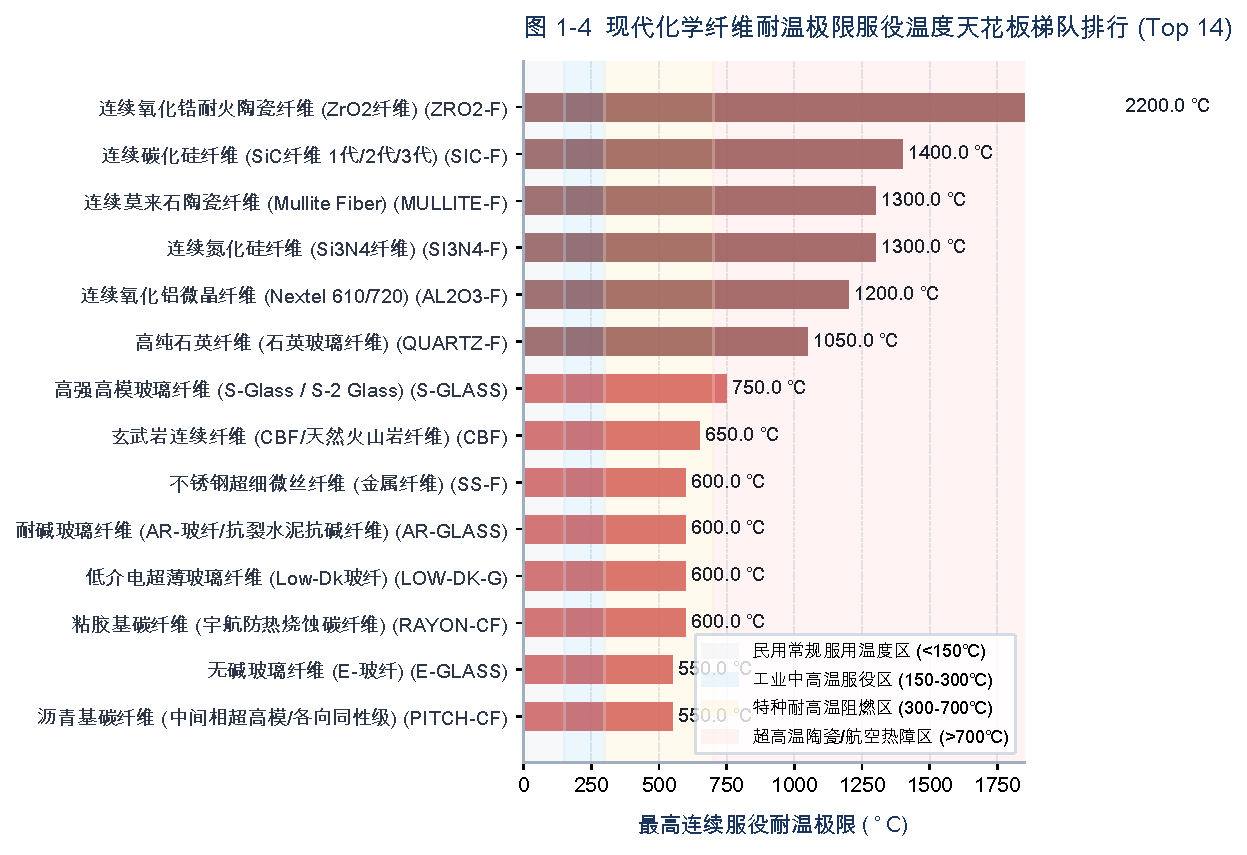
\includegraphics[width=0.92\textwidth]{figures/fig4_service_temp_ladder.pdf}
\caption{现代化学纤维耐温极限服役温度天花板梯队排行 (Top 14)}
\label{fig:temp_ladder}
\end{figure}

如图 \ref{fig:temp_ladder} 所示，从常规涤纶锦纶的 $150^\circ\mathrm{C}$，到间位芳纶 Nomex 的 $220^\circ\mathrm{C}$，再到玄武岩纤维的 $700^\circ\mathrm{C}$ 与碳化硅、氧化锆陶瓷纤维的 $1300^\circ\mathrm{C}-1600^\circ\mathrm{C}$，形成了分层严密的耐热屏障梯度体系。

\chapter{现代纺织经典混纺配伍与协同矩阵 (12大黄金配比)}

单一纤维通常存在性能短板，现代面料工程通过多组分短纤混纺或长丝交织实现协同互补：

\begin{academicblendbox}{配伍方案 1：涤棉混纺 (T/C \& CVC 混纺)}
\begin{itemize} \setlength{\itemsep}{2pt}
    \item \textbf{纤维组分构成}：PET聚酯纤维 (涤纶) + 天然棉纤维 (长绒棉/细绒棉)
    \item \textbf{经典黄金配比}：\texttt{T/C 65/35 (涤主) 或 CVC 60/40 (棉主)}
    \item \textbf{协同互补优势}：黄金互补：涤纶赋予面料极佳的断裂强力、抗皱保形性、耐磨损性与机洗免烫；棉纤维赋予高吸湿透气性、亲肤舒适感与消除静电积聚。
    \item \textbf{典型面料服饰}：经典男士正装商务衬衫、医院医护防静电白大褂、高强度耐洗工装制服、军训作训服、星级酒店耐洗床单被套。
    \item \textbf{染整关键与工艺策略}：分散染料染涤纶(130$^\circ\mathrm{C}$高温高压) + 活性染料染棉(60$^\circ\mathrm{C}$中温弱碱)，采用一浴两步法或两浴两步法连续轧染，控制热定型温度180-185$^\circ\mathrm{C}$以防棉泛黄脆损。
\end{itemize}
\end{academicblendbox}

\begin{academicblendbox}{配伍方案 2：涤粘混纺 (T/R 仿毛西服面料)}
\begin{itemize} \setlength{\itemsep}{2pt}
    \item \textbf{纤维组分构成}：PET聚酯纤维 (涤纶) + 粘胶纤维 (人造棉/人造丝)
    \item \textbf{经典黄金配比}：\texttt{T/R 65/35 或 T/R 70/30}
    \item \textbf{协同互补优势}：仿毛性价比之王：粘胶纤维有效消除涤纶静电、改善吸湿排汗手感并带来优雅悬垂感；涤纶提供永久褶裥记忆、高抗皱弹性与耐洗耐磨寿命。
    \item \textbf{典型面料服饰}：春秋季男女商务西服套装、男女职业西裤、百褶学生制服裙、免烫工装风衣。
    \item \textbf{染整关键与工艺策略}：分散染料染涤 + 活性/直接染料染粘胶，水洗缩水率控制在2\%以内，整理时加入抗起毛起球有机硅柔软剂改善手感。
\end{itemize}
\end{academicblendbox}

\begin{academicblendbox}{配伍方案 3：棉莫混纺 (Cotton / Modal 高端针织)}
\begin{itemize} \setlength{\itemsep}{2pt}
    \item \textbf{纤维组分构成}：精梳天然棉 (Combed Cotton) + 莫代尔纤维 (Modal)
    \item \textbf{经典黄金配比}：\texttt{50/50 或 60/40}
    \item \textbf{协同互补优势}：极致贴身享受：莫代尔赋予面料丝滑软糯手感、天然光泽和持久鲜艳色泽，克服纯棉多次水洗后发硬板结缺陷；棉纤维提高湿态稳定性和骨感挺括度。
    \item \textbf{典型面料服饰}：轻奢贴身无痕内衣、高端家居睡衣、夏日丝滑T恤、婴幼儿A类贴身连体衣、轻柔针织床品。
    \item \textbf{染整关键与工艺策略}：活性染料中温一浴法均染（二者均为纤维素同类染色），染色极性均匀，注意严格控制碱剂浓度防止莫代尔在强碱下过度溶胀。
\end{itemize}
\end{academicblendbox}

\begin{academicblendbox}{配伍方案 4：羊毛/腈纶混纺 (Wool / Acrylic 毛纺经典)}
\begin{itemize} \setlength{\itemsep}{2pt}
    \item \textbf{纤维组分构成}：天然绵羊毛 (Wool) + 聚丙烯腈纤维 (膨体腈纶)
    \item \textbf{经典黄金配比}：\texttt{70/30 (毛为主) 或 50/50 (平价毛线)}
    \item \textbf{协同互补优势}：保暖与抗缩绒协同：羊毛提供天然卷曲、高保暖性和高回弹性；腈纶（人造羊毛）显著降低面料自重，克服羊毛机洗毡缩起球缺点，降低原料成本且色彩更鲜亮。
    \item \textbf{典型面料服饰}：粗纺呢绒大衣面料、秋冬针织毛衣开衫、保暖围巾围脖、毛线手工编织纱线。
    \item \textbf{染整关键与工艺策略}：酸性染料(染羊毛) + 阳离子染料(染腈纶)，同浴两步法染色，严格防止两类阴阳电荷染料在水相中发生沉淀凝结，需加入非离子抗凝聚防沉淀剂。
\end{itemize}
\end{academicblendbox}

\begin{academicblendbox}{配伍方案 5：锦棉混纺 (Nylon / Cotton 户外高耐磨工装)}
\begin{itemize} \setlength{\itemsep}{2pt}
    \item \textbf{纤维组分构成}：聚酰胺长丝/短纤 (锦纶/尼龙) + 天然精梳棉
    \item \textbf{经典黄金配比}：\texttt{N/C 50/50 或 锦纶25\% + 棉75\%}
    \item \textbf{协同互补优势}：硬核防撕裂：锦纶的耐磨性是棉纤维的10倍、聚酯的2-3倍，赋予织物极高撕破强力与耐摩擦性；棉纤维保证剧烈运动出汗时的吸汗透气和舒适透气。
    \item \textbf{典型面料服饰}：美军战术作战服(ACU/BDU)、户外攀岩耐磨裤、高档冲锋衣内胆、工装多袋风衣、重型露营帐篷。
    \item \textbf{染整关键与工艺策略}：弱酸性染料染锦纶 + 活性染料染棉，热定型温度170-175$^\circ\mathrm{C}$，通常采用格纹防撕裂组织(Ripstop)织造。
\end{itemize}
\end{academicblendbox}

\begin{academicblendbox}{配伍方案 6：氨纶包芯纱高弹牛仔体系 (Core-Spun Spandex Denim)}
\begin{itemize} \setlength{\itemsep}{2pt}
    \item \textbf{纤维组分构成}：聚氨酯弹性纤维 (氨纶Spandex) 芯丝 + 外包纯棉或棉涤短纤
    \item \textbf{经典黄金配比}：\texttt{棉 95\%-98\% + 氨纶 2\%-5\%}
    \item \textbf{协同互补优势}：随形而动与自然棉感：中心氨纶提供 25\%-40\% 的舒适拉伸回复弹性与低滞后损耗，外层纯棉确保手感干爽纯正、支持经典靛蓝染色与洗水磨白落色效果。
    \item \textbf{典型面料服饰}：弹力紧身牛仔裤、四面弹修身休闲裤、高弹修身衬衫、运动打底紧身衣。
    \item \textbf{染整关键与工艺策略}：关键在后整理拉幅定型控制热定型温度（通常185-190$^\circ\mathrm{C}$保持30-40秒），避免过度高温使氨纶断裂老化丧失回弹性。
\end{itemize}
\end{academicblendbox}

\begin{academicblendbox}{配伍方案 7：天丝/亚麻混纺 (Lyocell / Linen 凉爽夏布)}
\begin{itemize} \setlength{\itemsep}{2pt}
    \item \textbf{纤维组分构成}：莱赛尔纤维 (天丝Lyocell) + 天然亚麻 (Flax/Linen)
    \item \textbf{经典黄金配比}：\texttt{天丝 70\% + 亚麻 30\% 或 50/50}
    \item \textbf{协同互补优势}：刚柔并济：亚麻具有天然粗犷竹节纹理、高导热凉感和干爽吸汗性能，但纯麻易刺痒、易褶皱发硬；天丝的加入赋予面料丝滑柔和触感与高悬垂抗皱性。
    \item \textbf{典型面料服饰}：高端度假风衬衫、夏季轻薄阔腿裤、法式文艺连衣裙、透气防晒风衣、天然凉爽夏被。
    \item \textbf{染整关键与工艺策略}：活性染料同浴染色，采用气流柔软机整理以充分消除粗麻纤维刺痒感，保留织物表面自然微竹节纹理。
\end{itemize}
\end{academicblendbox}

\begin{academicblendbox}{配伍方案 8：涤锦橘瓣复合超细纤维体系 (PET / PA Splittable Microfiber)}
\begin{itemize} \setlength{\itemsep}{2pt}
    \item \textbf{纤维组分构成}：PET聚酯裂片 (80\%) + PA6锦纶裂片 (20\%) 橘瓣相间复合
    \item \textbf{经典黄金配比}：\texttt{PET 80\% + PA6 20\%}
    \item \textbf{协同互补优势}：微观毛细管力风暴：水刺或碱处理将双组分剥离成0.1-0.2 dtex微纤，聚酯疏水刮擦除油污、锦纶微亲水吸水，截面毛细管密度增加数倍，产生强劲物理吸附效应。
    \item \textbf{典型面料服饰}：高吸水干发毛巾、光学精密仪器洁净擦拭布、高吸液运动毛巾、高密防风防水滑雪服。
    \item \textbf{染整关键与工艺策略}：先开纤后染色，分散染料染PET组分，酸性染料染PA组分，通常直接利用PET组分吸色或双色同色染色。
\end{itemize}
\end{academicblendbox}

\begin{academicblendbox}{配伍方案 9：羊绒/蚕丝/铜氨高定混纺 (Cashmere / Silk / Cupro Luxury Blend)}
\begin{itemize} \setlength{\itemsep}{2pt}
    \item \textbf{纤维组分构成}：山羊绒 (Cashmere) + 桑蚕丝 (Mulberry Silk) + 铜氨纤维 (Cupro)
    \item \textbf{经典黄金配比}：\texttt{羊绒 50\% + 蚕丝 30\% + 铜氨 20\%}
    \item \textbf{协同互补优势}：顶级奢华与呼吸感：羊绒提供极致轻盈蓄热软糯感，天然蚕丝赋予珍珠般光泽与滑糯，铜氨纤维消除静电、赋予丝滑透气与内衬呼吸般的湿热平衡。
    \item \textbf{典型面料服饰}：顶级高定时装大衣、奢华晚礼服、高档双面呢绒披风、手工定制贴肤围巾。
    \item \textbf{染整关键与工艺策略}：极温和弱酸性及中性低温染色，严禁强机械揉搓与剧烈碱性水洗，整理采用蒸汽轻柔松弛整理。
\end{itemize}
\end{academicblendbox}

\begin{academicblendbox}{配伍方案 10：芳纶阻燃防电弧安全工装混纺 (Nomex IIIA 永久防护混纺)}
\begin{itemize} \setlength{\itemsep}{2pt}
    \item \textbf{纤维组分构成}：间位芳纶 (PMIA 93\%) + 对位芳纶 (PPTA 5\%) + 导电碳芯微丝 (2\%)
    \item \textbf{经典黄金配比}：\texttt{93 / 5 / 2 (Nomex IIIA 国际标准配方)}
    \item \textbf{协同互补优势}：生命防护盾：间位芳纶耐热370$^\circ\mathrm{C}$离火自熄；5\%对位芳纶作为骨架支撑高温爆燃时不破洞不收缩；2\%导电纤维瞬间导除摩擦静电，防止引发易燃易爆气体爆燃。
    \item \textbf{典型面料服饰}：中石油/中石化加油与炼油防静电阻燃服、国家电网带电检修防电弧服、消防战斗服外层面料、军用战车阻燃服。
    \item \textbf{染整关键与工艺策略}：由于全芳香链难染，通常采用原液着色(Dope-dyed)长丝短纤，或在载体助剂存在下高压特种染整，色牢度达5级极值。
\end{itemize}
\end{academicblendbox}

\begin{academicblendbox}{配伍方案 11：竹浆/棉/莫代尔三合一家纺混纺 (Bamboo / Cotton / Modal Home Textile)}
\begin{itemize} \setlength{\itemsep}{2pt}
    \item \textbf{纤维组分构成}：竹浆粘胶纤维 (40\%) + 精梳长绒棉 (30\%) + 莫代尔 (30\%)
    \item \textbf{经典黄金配比}：\texttt{40 / 30 / 30}
    \item \textbf{协同互补优势}：生态抑菌与丝滑呼吸：竹浆纤维自带天然多孔吸湿和抑菌清爽感，棉提供洗涤骨架耐磨性，莫代尔赋予光泽和柔垂质感，三者融合带来云朵般睡眠体感。
    \item \textbf{典型面料服饰}：高端抗菌床品四件套、抑菌柔巾、酒店豪华浴巾、夏日凉感睡眠薄毯。
    \item \textbf{染整关键与工艺策略}：纤维素系环保活性染料一浴法染色，采用无张力松弛烘干工艺确保织物蓬松透气度。
\end{itemize}
\end{academicblendbox}

\begin{academicblendbox}{配伍方案 12：防切割5级特种复合装甲包覆纱 (Cut-Resistant Level 5 Armored Yarn)}
\begin{itemize} \setlength{\itemsep}{2pt}
    \item \textbf{纤维组分构成}：超高分子量聚乙烯(UHMWPE) + 超细微不锈钢丝/玻纤微丝 + 涤纶外包 + 氨纶芯丝
    \item \textbf{经典黄金配比}：\texttt{UHMWPE 55\% + 不锈钢丝 20\% + 涤纶 20\% + 氨纶 5\%}
    \item \textbf{协同互补优势}：机械刃具物理阻隔：中心不锈钢丝直接钝化刀刃锋利尖端，UHMWPE高断裂强力与抗撕裂延展性吸收切割动能，外层涤纶抗磨损，氨纶赋予手套灵活穿戴抓握感。
    \item \textbf{典型面料服饰}：EN 388最高防切割5级工业防护手套、屠宰流水线防刺防割衣、警用防暴防割战术手套、玻璃搬运防护服。
    \item \textbf{染整关键与工艺策略}：空心锭精密双向包覆纱机加工，UHMWPE原液着色，无需高温水染，整理主要为针织成型后浸渍PU或丁腈橡胶涂层。
\end{itemize}
\end{academicblendbox}

\chapter{国际生态纺织品标准与绿色合规体系}

现代纺织供应链已全面迈入可追溯、无害化与低碳化时代：

\begin{itemize}
    \item \textbf{OEKO-TEX® Standard 100}：全球最权威的纺织品生态安全认证，分为 Product Class I（婴幼儿安全级，甲醛零检出、pH弱酸性、重金属严格受限）、Class II（直接接触皮肤级）、Class III（非直接接触皮肤级）与 Class IV（装饰材料级）。
    \item \textbf{GRS (Global Recycled Standard 全球回收标准)}：针对消费后塑料瓶片（rPET）或废旧纺织品循环再生的国际全链条自愿性标准，严格审查原料回收真实性、TC 交易凭证、环境污水管控与企业社会责任。
    \item \textbf{Bluesign® 蓝标体系}：从纺织产业链的最前端（化学品原料输入）实施严格筛查，消除对人类健康和生态水质有危害的化学助剂。
    \item \textbf{ZDHC (零排放有害化学品)}：推动国际主流纺织服装品牌供应链在印染后整理中淘汰致癌芳香胺、全氟辛酸(PFOA/PFOS)及重金属媒染剂。
    \item \textbf{产品碳足迹 (ISO 14067)}：科学测算从聚合物原料开采、纺丝、织造到成衣消费端全生命周期的温室气体排放。
\end{itemize}

\part{再生纤维与人造天然聚合物纤维 (Regenerated \& Natural Polymer Fibers)}

\chapter{再生纤维素纤维 (REG\_CELL)}
\begin{quote}
\small\itshape
包括传统粘胶法、铜氨法、环保NMMO溶剂法(莱赛尔)、离子液体法及醋酸纤维素
\end{quote}

\section{粘胶纤维 (普通粘胶/人造棉/人造丝) [CV]}
\label{sec:cv}

\noindent\textbf{英文通用名称}：\textit{Viscose Rayon}\par
\noindent\textbf{工程应用标签}：\texttt{纺织门类: 服装用纺织品 / 家用纺织品 | 生物基原料 | 环境生物降解}\par
\noindent\textbf{历史工业化历程}：第1代人造纤维 · 实验室发现年代：\texttt{1891} · 商业化量产：\texttt{1905} · 先驱机构：Cross, Bevan \& Beadle (英国 Courtaulds)\par
\noindent\textbf{化学命名与分子式}：再生纤维素 (黄原酸酯法) · 分子式：\texttt{(C6H10O5)n} · CAS 号：\texttt{68442-85-3}\par
\noindent\textbf{成型与拉伸工艺}：湿法纺丝 (硫酸/硫酸锌/硫酸钠酸浴凝固)\par

\vspace{0.15cm}
\begin{center}
\small
\begin{tabularx}{\textwidth}{p{3.8cm}Xp{3.8cm}X}
\toprule
\textbf{基础物化指标} & \textbf{工程参考值} & \textbf{基础物化指标} & \textbf{工程参考值} \\
\midrule
晶体密度 (Density) & 1.51 g/cm$^3$ & 断裂拉伸强度 (Strength) & 0.33 GPa (2.2 cN/dtex) \\
拉伸初始模量 (Modulus) & 5.5 GPa & 断裂伸长率 (Elongation) & 20.0 \% \\
公定回潮率 (Moisture) & \textbf{13.0 \%} & 极限氧指数 (LOI) & \textbf{19.5 \%} \\
熔点 / 热分解点 (Melt) & 不熔/碳化 $^\circ\mathrm{C}$ & 长期连续服役耐温 & 120.0 $^\circ\mathrm{C}$ \\
\bottomrule
\end{tabularx}
\end{center}
\vspace{0.15cm}

\begin{academicbox}{现代纺织工程技术与面料应用学术档案}
\small
\begin{itemize} \setlength{\itemsep}{2.5pt}
    \item \textbf{微观截面几何形态}：\texttt{锯齿形边缘，明显皮芯层结构 (Serrated skin-core)}
    \item \textbf{纺织细度指标范围}：1.33 - 3.3 dtex (棉型短纤/中长短纤)；40D - 120D (人造丝长丝)
    \item \textbf{纱线加工技术规格}：人棉纱 (21S-60S), 粘胶长丝 (Rayon filament), 涡流纺气流纺纱
    \item \textbf{手感风格与悬垂触感}：吸湿滑糯、悬垂性极佳、透气清凉、亲肤无静电、抗起毛起球好
    \item \textbf{印染工艺与适用染料}：活性染料、直接染料、还原染料均可在温和弱碱中易染，得色饱满鲜艳，均染性好
    \item \textbf{耐洗与日晒色牢度等级}：\texttt{耐洗 3-4 级；日晒 3-4 级}
    \item \textbf{热湿舒适与导湿机制}：公定回潮率高达 13.0\% (远高于棉的8.5\%)；吸湿透气极度清爽，消除静电电荷
    \item \textbf{抗起球级数与耐磨评级}：\texttt{抗起球性极佳 (4-5 级，起球极少)；湿态强力下降约 40\%-50\%（需防湿态强揉搓）}
    \item \textbf{弹性伸长与抗皱保形}：急弹性较差，湿态容易褶皱缩水（普通人棉水洗缩水率 5\%-8\%）
    \item \textbf{经典混纺推荐与协同}：\textbf{粘胶 + 涤纶 (T/R 65/35 仿毛西服)；粘胶 + 锦纶 (增加耐磨性)；粘胶 + 棉 (吸湿舒适)}
    \item \textbf{适用织造与编织工艺}：圆机人棉汗布、人造丝提花里料织造、水刺无纺布湿巾
    \item \textbf{洗涤保养与熨烫要点}：轻柔水洗或干洗，水温\textless{}40$^\circ\mathrm{C}$；避免死力拧干；中温熨烫 (\textless{}140$^\circ\mathrm{C}$) 恢复平整
    \item \textbf{国际生态纺织认证}：\texttt{OEKO-TEX Standard 100, FSC 森林浆粕可持续认证}
\end{itemize}
\end{academicbox}

\noindent\textbf{【商标与别名】}：\texttt{Rayon}、\texttt{人造棉}、\texttt{人造丝}、\texttt{粘纤}、\texttt{CV}\par
\noindent\textbf{【代表性商业品牌】}：Danufil, Rayon, 人造丝, 人造棉\par
\noindent\textbf{【典型终端应用场景】}：服装内衣、面料衬里、家用纺织品、医用纱布水刺无纺布、湿巾\par
\noindent\textbf{【2026年产业化与成熟度进展】}：产业规模成熟；全面升级为密闭化二硫化碳全回收环保生产线与循环再生棉浆粕源\par
\noindent\textbf{【引用标准规范】}：[ISO] \texttt{ISO 2076:2021}; [GB] \texttt{GB/T 4146.1-2020}\par
\vspace{0.5cm}

\section{莫代尔纤维 (高湿模量粘胶纤维) [CMD]}
\label{sec:cmd}

\noindent\textbf{英文通用名称}：\textit{Modal Fiber}\par
\noindent\textbf{工程应用标签}：\texttt{纺织门类: 服装用纺织品 / 家用纺织品 | 生物基原料 | 环境生物降解}\par
\noindent\textbf{历史工业化历程}：第2代差别化纤维 · 实验室发现年代：\texttt{1951} · 商业化量产：\texttt{1960s} · 先驱机构：Tachikawa (日本立川) / 兰精 (Lenzing)\par
\noindent\textbf{化学命名与分子式}：高湿模量改性再生纤维素 · 分子式：\texttt{(C6H10O5)n} · CAS 号：\texttt{68442-85-3}\par
\noindent\textbf{成型与拉伸工艺}：改性湿法纺丝 (慢凝固浴、高拉伸低酸工艺)\par

\vspace{0.15cm}
\begin{center}
\small
\begin{tabularx}{\textwidth}{p{3.8cm}Xp{3.8cm}X}
\toprule
\textbf{基础物化指标} & \textbf{工程参考值} & \textbf{基础物化指标} & \textbf{工程参考值} \\
\midrule
晶体密度 (Density) & 1.52 g/cm$^3$ & 断裂拉伸强度 (Strength) & 0.52 GPa (3.4 cN/dtex) \\
拉伸初始模量 (Modulus) & 7.0 GPa & 断裂伸长率 (Elongation) & 14.0 \% \\
公定回潮率 (Moisture) & \textbf{12.5 \%} & 极限氧指数 (LOI) & \textbf{19.5 \%} \\
熔点 / 热分解点 (Melt) & 不熔/碳化 $^\circ\mathrm{C}$ & 长期连续服役耐温 & 130.0 $^\circ\mathrm{C}$ \\
\bottomrule
\end{tabularx}
\end{center}
\vspace{0.15cm}

\begin{academicbox}{现代纺织工程技术与面料应用学术档案}
\small
\begin{itemize} \setlength{\itemsep}{2.5pt}
    \item \textbf{微观截面几何形态}：\texttt{近圆形或腰子形，全皮层或均质无皮芯微观结构}
    \item \textbf{纺织细度指标范围}：1.0 - 1.33 dtex (精梳棉型高湿模量短纤)
    \item \textbf{纱线加工技术规格}：紧密赛络纺短纤纱 (40S-100S 高支纱), 针织股线
    \item \textbf{手感风格与悬垂触感}：软糯似羊绒、悬垂如瀑布、丝般光泽细腻、越洗越柔软
    \item \textbf{印染工艺与适用染料}：活性染料染色，上染率高，色泽鲜亮均一，耐氯漂性好于普通粘胶
    \item \textbf{耐洗与日晒色牢度等级}：\texttt{耐洗 4 级；耐摩擦 4 级}
    \item \textbf{热湿舒适与导湿机制}：公定回潮率 12.5\%，干湿强度比高（湿强达到干强的 60\% 以上），吸汗透湿极佳
    \item \textbf{抗起球级数与耐磨评级}：\texttt{抗起球 3-4 级；洗涤后不发硬、不变脆}
    \item \textbf{弹性伸长与抗皱保形}：抗皱保形性显著优于普通粘胶，水洗缩水率低 (\textless{}3\%)
    \item \textbf{经典混纺推荐与协同}：\textbf{莫代尔 + 精梳棉 (50/50 顶级内衣黄金混纺)；莫代尔 + 氨纶 (弹力针织贴身面料)}
    \item \textbf{适用织造与编织工艺}：高密单双面大圆机针织、高端床品机织大提花
    \item \textbf{洗涤保养与熨烫要点}：常规机洗，水温 40$^\circ\mathrm{C}$，无需特殊护理，洗后自然平整垂坠
    \item \textbf{国际生态纺织认证}：\texttt{OEKO-TEX 100 Class I, EU Ecolabel (欧盟生态之花认证)}
\end{itemize}
\end{academicbox}

\noindent\textbf{【商标与别名】}：\texttt{Modal}、\texttt{木代尔}、\texttt{高湿模量粘胶}、\texttt{CMD}\par
\noindent\textbf{【代表性商业品牌】}：Lenzing Modal, MicroModal\par
\noindent\textbf{【典型终端应用场景】}：高档贴身内衣、床品家纺、高支针织面料、柔顺亲肤混纺纺织品\par
\noindent\textbf{【2026年产业化与成熟度进展】}：全球高档纺织核心原料，广泛结合环保认证榉木浆与零碳碳中和认证\par
\noindent\textbf{【引用标准规范】}：[GB] \texttt{GB/T 22704-2019}; [ISO] \texttt{ISO 2076:2021}\par
\vspace{0.5cm}

\section{莱赛尔纤维 (天丝/溶剂法纤维素纤维) [CLY]}
\label{sec:cly}

\noindent\textbf{英文通用名称}：\textit{Lyocell Fiber}\par
\noindent\textbf{工程应用标签}：\texttt{纺织门类: 服装用纺织品 / 家用纺织品 | 生物基原料 | 环境生物降解}\par
\noindent\textbf{历史工业化历程}：第3代绿色人造纤维 · 实验室发现年代：\texttt{1972} · 商业化量产：\texttt{1992} · 先驱机构：Akzo Nobel / Courtaulds / Lenzing\par
\noindent\textbf{化学命名与分子式}：N-甲基氧化吗啉 (NMMO) 溶剂法再生纤维素 · 分子式：\texttt{(C6H10O5)n} · CAS 号：\texttt{68442-85-3}\par
\noindent\textbf{成型与拉伸工艺}：干湿法纺丝 (NMMO水溶液直接物理溶解，溶剂回收率\textgreater{}99.5\%)\par

\vspace{0.15cm}
\begin{center}
\small
\begin{tabularx}{\textwidth}{p{3.8cm}Xp{3.8cm}X}
\toprule
\textbf{基础物化指标} & \textbf{工程参考值} & \textbf{基础物化指标} & \textbf{工程参考值} \\
\midrule
晶体密度 (Density) & 1.5 g/cm$^3$ & 断裂拉伸强度 (Strength) & 0.63 GPa (4.2 cN/dtex) \\
拉伸初始模量 (Modulus) & 11.0 GPa & 断裂伸长率 (Elongation) & 13.0 \% \\
公定回潮率 (Moisture) & \textbf{11.5 \%} & 极限氧指数 (LOI) & \textbf{20.0 \%} \\
熔点 / 热分解点 (Melt) & 不熔/碳化 $^\circ\mathrm{C}$ & 长期连续服役耐温 & 140.0 $^\circ\mathrm{C}$ \\
\bottomrule
\end{tabularx}
\end{center}
\vspace{0.15cm}

\begin{academicbox}{现代纺织工程技术与面料应用学术档案}
\small
\begin{itemize} \setlength{\itemsep}{2.5pt}
    \item \textbf{微观截面几何形态}：\texttt{极规整平滑的光滑圆形截面，无皮芯层均质结构}
    \item \textbf{纺织细度指标范围}：1.33 - 1.7 dtex (常规天丝)；1.0 - 1.2 dtex (细旦天丝)
    \item \textbf{纱线加工技术规格}：天丝纯纺纱 (30S-80S), 天丝长丝 (Lyocell Filament), 赛络紧密纺
    \item \textbf{手感风格与悬垂触感}：凉爽爽滑、真丝般光泽、悬垂挺顺、具有天然桃皮绒触感(原纤化风格)
    \item \textbf{印染工艺与适用染料}：对活性染料亲和力极强，上染速度快，深色丰满纯正，节约染料染剂20\%
    \item \textbf{耐洗与日晒色牢度等级}：\texttt{耐水洗 4-5 级；耐湿摩擦 3-4 级}
    \item \textbf{热湿舒适与导湿机制}：回潮率 11.5\%，具有出色的湿热调节呼吸能力，菌落附着率仅为合成纤维的千分之一
    \item \textbf{抗起球级数与耐磨评级}：\texttt{常规型在湿态机械摩擦下易产生微原纤化（桃皮绒手感），需防过度起白霜}
    \item \textbf{弹性伸长与抗皱保形}：干强与湿强俱极高（湿态强力达到干态 85\%，远超粘胶与棉），保形性优秀
    \item \textbf{经典混纺推荐与协同}：\textbf{莱赛尔 + 亚麻 (70/30 凉爽抗皱夏装)；莱赛尔 + 棉 (60/40 亲肤家纺)；莱赛尔 + 蚕丝}
    \item \textbf{适用织造与编织工艺}：高支高密喷气机织床品、牛仔布斜纹织造、高端女装轻薄机织面料
    \item \textbf{洗涤保养与熨烫要点}：30-40$^\circ\mathrm{C}$轻柔机洗，反面洗涤，防止剧烈摩擦产生白霜，中温蒸汽熨烫
    \item \textbf{国际生态纺织认证}：\texttt{闭环绿色工艺 (NMMO回收率\textgreater{}99.7\%), OEKO-TEX 100, 欧盟生态标签}
\end{itemize}
\end{academicbox}

\noindent\textbf{【商标与别名】}：\texttt{Tencel}、\texttt{天丝}、\texttt{溶剂法纤维素纤维}、\texttt{CLY}\par
\noindent\textbf{【代表性商业品牌】}：Tencel (天丝), Lenzing Lyocell, 中纺院绿纤\par
\noindent\textbf{【典型终端应用场景】}：中高端服装面料、牛仔服饰、水刺高级医美无纺布、电池隔膜纸基材料\par
\noindent\textbf{【2026年产业化与成熟度进展】}：绿色纤维主导品种，百万吨级产能落地，原纤化调控与非原纤化改性技术全面成熟\par
\noindent\textbf{【引用标准规范】}：[GB] \texttt{GB/T 22703-2008}; [ISO] \texttt{ISO 2076:2021}\par
\vspace{0.5cm}

\section{铜氨纤维 [CUP]}
\label{sec:cup}

\noindent\textbf{英文通用名称}：\textit{Cupro (Cuprammonium Rayon)}\par
\noindent\textbf{工程应用标签}：\texttt{纺织门类: 服装用纺织品 / 家用纺织品 | 生物基原料 | 环境生物降解}\par
\noindent\textbf{历史工业化历程}：第1代人造纤维 · 实验室发现年代：\texttt{1897} · 商业化量产：\texttt{1919} · 先驱机构：Bemberg (宾霸 / 旭化成 Asahi Kasei)\par
\noindent\textbf{化学命名与分子式}：氢氧化四氨合铜络合物溶剂法再生纤维素 · 分子式：\texttt{(C6H10O5)n} · CAS 号：\texttt{68442-85-3}\par
\noindent\textbf{成型与拉伸工艺}：漏斗式湿法喷丝成形 (铜氨络合物水溶液溶解棉短绒)\par

\vspace{0.15cm}
\begin{center}
\small
\begin{tabularx}{\textwidth}{p{3.8cm}Xp{3.8cm}X}
\toprule
\textbf{基础物化指标} & \textbf{工程参考值} & \textbf{基础物化指标} & \textbf{工程参考值} \\
\midrule
晶体密度 (Density) & 1.52 g/cm$^3$ & 断裂拉伸强度 (Strength) & 0.35 GPa (2.3 cN/dtex) \\
拉伸初始模量 (Modulus) & 6.5 GPa & 断裂伸长率 (Elongation) & 18.0 \% \\
公定回潮率 (Moisture) & \textbf{12.0 \%} & 极限氧指数 (LOI) & \textbf{20.0 \%} \\
熔点 / 热分解点 (Melt) & 不熔/碳化 $^\circ\mathrm{C}$ & 长期连续服役耐温 & 125.0 $^\circ\mathrm{C}$ \\
\bottomrule
\end{tabularx}
\end{center}
\vspace{0.15cm}

\begin{academicbox}{现代纺织工程技术与面料应用学术档案}
\small
\begin{itemize} \setlength{\itemsep}{2.5pt}
    \item \textbf{微观截面几何形态}：\texttt{极其均匀光滑的正圆形，无皮芯层结构}
    \item \textbf{纺织细度指标范围}：0.5 - 1.3 dtex (超细旦铜氨长丝，如 30D/30f, 50D/48f)
    \item \textbf{纱线加工技术规格}：铜氨长丝 (Cupro Filament / 宾霸丝 Bemberg), 极细高支短纤
    \item \textbf{手感风格与悬垂触感}：“会呼吸的丝绸”，丝滑无阻滞感、冰润清凉、极致柔垂、优雅弱光泽
    \item \textbf{印染工艺与适用染料}：活性染料、直接染料中低温染色，上染快、色泽沉稳深邃
    \item \textbf{耐洗与日晒色牢度等级}：\texttt{耐洗 3-4 级；干洗 4-5 级}
    \item \textbf{热湿舒适与导湿机制}：公定回潮率 11.0\%，能瞬间吸收体表微汗并向外散发，完全消除静电吸附（不吸附裙摆）
    \item \textbf{抗起球级数与耐磨评级}：\texttt{抗起球 4-5 级；织物表面极平滑防摩擦}
    \item \textbf{弹性伸长与抗皱保形}：悬垂自如，抗静电贴合人体曲线
    \item \textbf{经典混纺推荐与协同}：\textbf{铜氨长丝用于顶级羊毛西服/风衣内衬 (100\% Bemberg Lining)；铜氨 + 蚕丝交织}
    \item \textbf{适用织造与编织工艺}：高档西服里料多臂提花织造、仿真丝绸缎机织、高端针织睡裙
    \item \textbf{洗涤保养与熨烫要点}：高档成衣建议优质干洗或30$^\circ\mathrm{C}$轻柔手洗，平铺阴干，低温垫布熨烫 (\textless{}120$^\circ\mathrm{C}$)
    \item \textbf{国际生态纺织认证}：\texttt{GRS认证 (利用棉籽短绒副产物再生), 生物可降解认证, OEKO-TEX 100}
\end{itemize}
\end{academicbox}

\noindent\textbf{【商标与别名】}：\texttt{Bemberg}、\texttt{宾霸}、\texttt{铜氨丝}、\texttt{CUP}\par
\noindent\textbf{【代表性商业品牌】}：Bemberg (宾霸), Asahi Kasei Cupro\par
\noindent\textbf{【典型终端应用场景】}：奢华西服里料、高级真丝触感时装、透气面膜基布、超纯无尘擦拭布\par
\noindent\textbf{【2026年产业化与成熟度进展】}：以棉籽短绒为全降解原料的高端闭环制造，日本与中国新增高洁净化生产基地\par
\noindent\textbf{【引用标准规范】}：[GB] \texttt{FZ/T 52022-2012}; [ISO] \texttt{ISO 2076:2021}\par
\vspace{0.5cm}

\section{醋酯纤维 (二醋酸纤维) [CA]}
\label{sec:ca}

\noindent\textbf{英文通用名称}：\textit{Acetate Fiber (Cellulose Diacetate)}\par
\noindent\textbf{工程应用标签}：\texttt{纺织门类: 服装用纺织品 / 家用纺织品 | 生物基原料 | 环境生物降解}\par
\noindent\textbf{历史工业化历程}：第1代半合成纤维 · 实验室发现年代：\texttt{1865} · 商业化量产：\texttt{1924} · 先驱机构：Dreyfus 兄弟 (Celanese / 塞拉尼斯)\par
\noindent\textbf{化学命名与分子式}：二乙酰基纤维素酯 · 分子式：\texttt{[C6H7O2(OH)x(OOCCH3)y]n (y$\approx$2.4)} · CAS 号：\texttt{9004-35-7}\par
\noindent\textbf{成型与拉伸工艺}：干法纺丝 (丙酮溶剂溶解二醋酸纤维素，热空气挥发成形)\par

\vspace{0.15cm}
\begin{center}
\small
\begin{tabularx}{\textwidth}{p{3.8cm}Xp{3.8cm}X}
\toprule
\textbf{基础物化指标} & \textbf{工程参考值} & \textbf{基础物化指标} & \textbf{工程参考值} \\
\midrule
晶体密度 (Density) & 1.32 g/cm$^3$ & 断裂拉伸强度 (Strength) & 0.18 GPa (1.4 cN/dtex) \\
拉伸初始模量 (Modulus) & 3.8 GPa & 断裂伸长率 (Elongation) & 28.0 \% \\
公定回潮率 (Moisture) & \textbf{6.5 \%} & 极限氧指数 (LOI) & \textbf{18.5 \%} \\
熔点 / 热分解点 (Melt) & 260.0 $^\circ\mathrm{C}$ & 长期连续服役耐温 & 110.0 $^\circ\mathrm{C}$ \\
\bottomrule
\end{tabularx}
\end{center}
\vspace{0.15cm}

\begin{academicbox}{现代纺织工程技术与面料应用学术档案}
\small
\begin{itemize} \setlength{\itemsep}{2.5pt}
    \item \textbf{微观截面几何形态}：\texttt{三叶形 / 多瓣凹槽形 (Trilobal / Multi-lobed)}
    \item \textbf{纺织细度指标范围}：55D - 150D (二醋酸长丝与短纤)
    \item \textbf{纱线加工技术规格}：醋酸长丝 (Acetate Filament), 醋酯混纺纱
    \item \textbf{手感风格与悬垂触感}：极度仿真丝手感、爽滑飘逸、悬垂性极佳、光泽高贵柔和、防静电不吸身
    \item \textbf{印染工艺与适用染料}：分散染料在 70-85$^\circ\mathrm{C}$ 温和染色，色光清透纯净，严禁强碱与沸腾剧烈洗练
    \item \textbf{耐洗与日晒色牢度等级}：\texttt{耐干洗 4-5 级；耐汗渍 4 级}
    \item \textbf{热湿舒适与导湿机制}：公定回潮率 6.5\%，具有天然纤维素呼吸透气感，穿着清凉不闷热
    \item \textbf{抗起球级数与耐磨评级}：\texttt{抗起球 4-5 级；耐磨性低于锦纶涤纶，适合高档礼服内衬}
    \item \textbf{弹性伸长与抗皱保形}：抗皱性优良，尺寸稳定性好，自然下垂恢复平整
    \item \textbf{经典混纺推荐与协同}：\textbf{二醋酸长丝与粘胶/涤纶交织做高档时装面料；100\%二醋酸用作高端风衣与西装里料}
    \item \textbf{适用织造与编织工艺}：多臂喷气丝织机、经编高档时装绸缎机织
    \item \textbf{洗涤保养与熨烫要点}：推荐专业优质干洗或30$^\circ\mathrm{C}$轻柔手洗，平铺晾干，严禁接触丙酮/香水等有机溶剂
    \item \textbf{国际生态纺织认证}：\texttt{OEKO-TEX Standard 100, 天然木浆生物基认证}
\end{itemize}
\end{academicbox}

\noindent\textbf{【商标与别名】}：\texttt{醋酸纤维}、\texttt{二醋酸}、\texttt{Celanese}、\texttt{CA}\par
\noindent\textbf{【代表性商业品牌】}：Celanese Acetate, Eastman Estron\par
\noindent\textbf{【典型终端应用场景】}：香烟滤嘴丝束、高端仿真丝礼服、轻奢围巾领带、女士缎面面料\par
\noindent\textbf{【2026年产业化与成熟度进展】}：滤嘴丝束全面推广可自然堆肥降解新型增塑剂配方，纺织领域向超细高回弹长丝扩展\par
\noindent\textbf{【引用标准规范】}：[GB] \texttt{GB/T 4146.1-2020}; [ISO] \texttt{ISO 2076:2021}\par
\vspace{0.5cm}

\section{三醋酯纤维 (三醋酸纤维) [CTA]}
\label{sec:cta}

\noindent\textbf{英文通用名称}：\textit{Triacetate Fiber (Cellulose Triacetate)}\par
\noindent\textbf{工程应用标签}：\texttt{纺织门类: 服装用纺织品 / 家用纺织品 | 生物基原料 | 环境生物降解}\par
\noindent\textbf{历史工业化历程}：第2代改性半合成纤维 · 实验室发现年代：\texttt{1894} · 商业化量产：\texttt{1954} · 先驱机构：Celanese / Courtaulds\par
\noindent\textbf{化学命名与分子式}：三乙酰基纤维素酯 · 分子式：\texttt{[C6H7O2(OOCCH3)3]n} · CAS 号：\texttt{9012-09-3}\par
\noindent\textbf{成型与拉伸工艺}：干法纺丝 (二氯甲烷/甲醇混合溶剂挥发)\par

\vspace{0.15cm}
\begin{center}
\small
\begin{tabularx}{\textwidth}{p{3.8cm}Xp{3.8cm}X}
\toprule
\textbf{基础物化指标} & \textbf{工程参考值} & \textbf{基础物化指标} & \textbf{工程参考值} \\
\midrule
晶体密度 (Density) & 1.3 g/cm$^3$ & 断裂拉伸强度 (Strength) & 0.16 GPa (1.2 cN/dtex) \\
拉伸初始模量 (Modulus) & 4.0 GPa & 断裂伸长率 (Elongation) & 25.0 \% \\
公定回潮率 (Moisture) & \textbf{3.5 \%} & 极限氧指数 (LOI) & \textbf{19.0 \%} \\
熔点 / 热分解点 (Melt) & 300.0 $^\circ\mathrm{C}$ & 长期连续服役耐温 & 130.0 $^\circ\mathrm{C}$ \\
\bottomrule
\end{tabularx}
\end{center}
\vspace{0.15cm}

\begin{academicbox}{现代纺织工程技术与面料应用学术档案}
\small
\begin{itemize} \setlength{\itemsep}{2.5pt}
    \item \textbf{微观截面几何形态}：\texttt{微多瓣三叶形 (三醋酯截面)}
    \item \textbf{纺织细度指标范围}：75D - 150D (三醋酸长丝)
    \item \textbf{纱线加工技术规格}：三醋酸高档时装长丝 (Triacetate Filament)
    \item \textbf{手感风格与悬垂触感}：近乎天然蚕丝的极致滑糯骨感、挺阔悬垂、珠光微泽、高贵奢华
    \item \textbf{印染工艺与适用染料}：分散染料高温高压染色 (120-130$^\circ\mathrm{C}$)，耐热耐洗性显著高于二醋酸
    \item \textbf{耐洗与日晒色牢度等级}：\texttt{耐水洗 4-5 级；耐摩擦 4 级}
    \item \textbf{热湿舒适与导湿机制}：回潮率 3.5\%，抗静电、吸湿排汗好，夏日贴身凉爽透气
    \item \textbf{抗起球级数与耐磨评级}：\texttt{抗起球 4-5 级；抗刮擦性显著优于真丝}
    \item \textbf{弹性伸长与抗皱保形}：免烫抗皱性能极佳，耐受高温热定型形成永久百褶裙裥
    \item \textbf{经典混纺推荐与协同}：\textbf{三醋酸 + 涤纶 (抗皱华丽礼服裙)；三醋酸 + 蚕丝 (高端新中式旗袍面料)}
    \item \textbf{适用织造与编织工艺}：高密丝织机缎纹、双绉织造、圆机醋酸针织面料
    \item \textbf{洗涤保养与熨烫要点}：支持轻柔机洗，耐受熨烫温度高达 200$^\circ\mathrm{C}$ (远胜二醋酸的120$^\circ\mathrm{C}$)，易打理不易泛黄
    \item \textbf{国际生态纺织认证}：\texttt{OEKO-TEX Standard 100, 绿色森林浆粕认证}
\end{itemize}
\end{academicbox}

\noindent\textbf{【商标与别名】}：\texttt{三醋酸}、\texttt{三醋酯}、\texttt{Soalon}、\texttt{CTA}\par
\noindent\textbf{【代表性商业品牌】}：Soalon (日本三菱化学), Arnel\par
\noindent\textbf{【典型终端应用场景】}：免烫高档西服、百褶裙、醋酸缎光礼服、光学偏光片保护膜前驱体\par
\noindent\textbf{【2026年产业化与成熟度进展】}：日本三菱化学独家技术持续垄断超高端时尚女装，环保非卤溶剂纺丝新产线落成\par
\noindent\textbf{【引用标准规范】}：[ISO] \texttt{ISO 2076:2021}; [GB] \texttt{GB/T 4146.1-2020}\par
\vspace{0.5cm}

\section{细菌纤维素纤维 [BC]}
\label{sec:bc}

\noindent\textbf{英文通用名称}：\textit{Bacterial Cellulose Fiber}\par
\noindent\textbf{工程应用标签}：\texttt{纺织门类: 服装用纺织品 / 家用纺织品 | 生物基原料 | 环境生物降解 | 战略特种高性能}\par
\noindent\textbf{历史工业化历程}：第4代生物工程合成纤维 · 实验室发现年代：\texttt{1886} · 商业化量产：\texttt{2010s} · 先驱机构：Brown / 现代合成生物学研究机构\par
\noindent\textbf{化学命名与分子式}：醋酸杆菌生物合成超微纯纤维素 · 分子式：\texttt{(C6H10O5)n} · CAS 号：\texttt{68442-85-3}\par
\noindent\textbf{成型与拉伸工艺}：生物反应发酵自组装网络，或微流控湿法定向纺丝\par

\vspace{0.15cm}
\begin{center}
\small
\begin{tabularx}{\textwidth}{p{3.8cm}Xp{3.8cm}X}
\toprule
\textbf{基础物化指标} & \textbf{工程参考值} & \textbf{基础物化指标} & \textbf{工程参考值} \\
\midrule
晶体密度 (Density) & 1.55 g/cm$^3$ & 断裂拉伸强度 (Strength) & 1.0 GPa (6.5 cN/dtex) \\
拉伸初始模量 (Modulus) & 25.0 GPa & 断裂伸长率 (Elongation) & 4.0 \% \\
公定回潮率 (Moisture) & \textbf{14.0 \%} & 极限氧指数 (LOI) & \textbf{20.0 \%} \\
熔点 / 热分解点 (Melt) & 不熔/碳化 $^\circ\mathrm{C}$ & 长期连续服役耐温 & 150.0 $^\circ\mathrm{C}$ \\
\bottomrule
\end{tabularx}
\end{center}
\vspace{0.15cm}

\begin{academicbox}{现代纺织工程技术与面料应用学术档案}
\small
\begin{itemize} \setlength{\itemsep}{2.5pt}
    \item \textbf{微观截面几何形态}：\texttt{三维超细纳米带状原纤网 (直径 20-100 nm 纳米纤维素网络)}
    \item \textbf{纺织细度指标范围}：纳米级原纤，单丝线密度 \textless{} 0.0001 dtex
    \item \textbf{纱线加工技术规格}：发酵成型湿态纳米凝胶水刺纤网、超微纳米保暖片材
    \item \textbf{手感风格与悬垂触感}：湿态呈果冻水凝胶状、极度亲肤柔嫩、服帖无气泡、干燥后高刚挺紧密
    \item \textbf{印染工艺与适用染料}：本白无添加直接应用，或载药生物敷料直接浸润
    \item \textbf{耐洗与日晒色牢度等级}：\texttt{医用生物纯净级}
    \item \textbf{热湿舒适与导湿机制}：超高保水保液率 (持水率达自重 100-200 倍)，透气不透菌，保持伤口湿性愈合
    \item \textbf{抗起球级数与耐磨评级}：\texttt{纳米网状纠缠抗拉强度极高（杨氏模量接近铝合金），耐牵拉不易撕裂}
    \item \textbf{弹性伸长与抗皱保形}：极佳三维形状追随性，紧密贴合人体皮肤微观纹理
    \item \textbf{经典混纺推荐与协同}：\textbf{细菌纤维素纳米网 + 壳聚糖/胶原蛋白 (复合医用人工皮肤敷料)}
    \item \textbf{适用织造与编织工艺}：静态生物发酵成膜、湿法复合抄纸成型
    \item \textbf{洗涤保养与熨烫要点}：医用一次性无菌包装，天然全生物降解
    \item \textbf{国际生态纺织认证}：\texttt{FDA 医疗器械生物相容性认证, ISO 10993}
\end{itemize}
\end{academicbox}

\noindent\textbf{【商标与别名】}：\texttt{BC纤维}、\texttt{生化纤维素}\par
\noindent\textbf{【代表性商业品牌】}：Biofibe, Nata de coco derived medical pulp\par
\noindent\textbf{【典型终端应用场景】}：人工血管移植管腔、高阶医用创面敷料、高端声学耳机振膜、柔性显示透明基底\par
\noindent\textbf{【2026年产业化与成熟度进展】}：生物反应器规模化量产达到千吨级，微流控连续拉伸制备高模长丝实现临床级体内植入认证\par
\noindent\textbf{【引用标准规范】}：[ASTM] \texttt{ASTM F3160-16}\par
\vspace{0.5cm}

\section{竹浆纤维 (竹粘胶纤维/竹素纤维) [BAMBOO]}
\label{sec:bamboo}

\noindent\textbf{英文通用名称}：\textit{Bamboo Pulp Viscose Fiber}\par
\noindent\textbf{工程应用标签}：\texttt{纺织门类: 服装用纺织品 / 家用纺织品 | 生物基原料 | 环境生物降解}\par
\noindent\textbf{历史工业化历程}：第2代特色天然生物质人造纤维 · 实验室发现年代：\texttt{1990s} · 商业化量产：\texttt{2002} · 先驱机构：吉林化纤 (天竹纤维)\par
\noindent\textbf{化学命名与分子式}：竹子纤维素经黄原酸酯法再生聚合物 · 分子式：\texttt{(C6H10O5)n} · CAS 号：\texttt{68442-85-3}\par
\noindent\textbf{成型与拉伸工艺}：湿法纺丝 (竹材粉碎蒸煮制浆、黄化溶解后湿法成形)\par

\vspace{0.15cm}
\begin{center}
\small
\begin{tabularx}{\textwidth}{p{3.8cm}Xp{3.8cm}X}
\toprule
\textbf{基础物化指标} & \textbf{工程参考值} & \textbf{基础物化指标} & \textbf{工程参考值} \\
\midrule
晶体密度 (Density) & 1.5 g/cm$^3$ & 断裂拉伸强度 (Strength) & 0.34 GPa (2.3 cN/dtex) \\
拉伸初始模量 (Modulus) & 5.8 GPa & 断裂伸长率 (Elongation) & 21.0 \% \\
公定回潮率 (Moisture) & \textbf{13.5 \%} & 极限氧指数 (LOI) & \textbf{19.5 \%} \\
熔点 / 热分解点 (Melt) & 不熔/碳化 $^\circ\mathrm{C}$ & 长期连续服役耐温 & 120.0 $^\circ\mathrm{C}$ \\
\bottomrule
\end{tabularx}
\end{center}
\vspace{0.15cm}

\begin{academicbox}{现代纺织工程技术与面料应用学术档案}
\small
\begin{itemize} \setlength{\itemsep}{2.5pt}
    \item \textbf{微观截面几何形态}：\texttt{椭圆形截面布满大小不一的微孔缝隙 (天然呼吸微气孔)}
    \item \textbf{纺织细度指标范围}：1.5 - 2.0 dtex (竹原短纤/竹浆短纤)
    \item \textbf{纱线加工技术规格}：竹纤维纯纺与混纺纱 (32S-60S), 提花毛巾长丝
    \item \textbf{手感风格与悬垂触感}：滑爽如丝、触感清凉细腻、悬垂优美、天然竹琨抑菌清香
    \item \textbf{印染工艺与适用染料}：活性染料常温中温染色，得色鲜亮纯正，吸色均匀快干
    \item \textbf{耐洗与日晒色牢度等级}：\texttt{耐洗 4 级；耐摩擦 4 级}
    \item \textbf{热湿舒适与导湿机制}：公定回潮率 13.0\%，微孔毛细横截面使其吸水排汗速度为棉的3倍，夏日吸汗极度清爽
    \item \textbf{抗起球级数与耐磨评级}：\texttt{抗起球 3-4 级；洗后柔软不板结}
    \item \textbf{弹性伸长与抗皱保形}：悬垂平顺，天然抗皱微回弹
    \item \textbf{经典混纺推荐与协同}：\textbf{竹浆纤维 60\% + 精梳棉 40\% (夏日爆款高吸水抑菌毛巾与凉感短袖T恤)}
    \item \textbf{适用织造与编织工艺}：单双面大圆机针织、剑杆提花毛巾机织造、凉感席面料
    \item \textbf{洗涤保养与熨烫要点}：常规家庭机洗，避免与尖锐金属拉链混洗防勾丝，中温熨烫
    \item \textbf{国际生态纺织认证}：\texttt{OEKO-TEX Standard 100, FSC 竹林可持续环保认证}
\end{itemize}
\end{academicbox}

\noindent\textbf{【商标与别名】}：\texttt{竹纤维}、\texttt{天竹}、\texttt{Tanboocel}\par
\noindent\textbf{【代表性商业品牌】}：Tanboocel (天竹 / 吉林化纤)\par
\noindent\textbf{【典型终端应用场景】}：天然抑菌毛巾、亲肤凉爽夏季凉席面料、竹纤维袜子内衣、卫生擦拭无纺布\par
\noindent\textbf{【2026年产业化与成熟度进展】}：绿色循环闭环清洁制浆技术全面升级，天然多孔横截面赋予其优异的透气排湿与抑菌防臭特性\par
\noindent\textbf{【引用标准规范】}：[GB] \texttt{GB/T 22705-2008}; [GB] \texttt{FZ/T 52010-2014}\par
\vspace{0.5cm}

\section{微纳原纤化纳米纤维素宏观连续纤维 (CNF长丝) [CNF-MACRO]}
\label{sec:cnf-macro}

\noindent\textbf{英文通用名称}：\textit{Cellulose Nanofiber Macrofilament (CNF Fiber)}\par
\noindent\textbf{工程应用标签}：\texttt{纺织门类: 服装用纺织品 / 家用纺织品 | 生物基原料 | 环境生物降解 | 战略特种高性能}\par
\noindent\textbf{历史工业化历程}：第4代全天然超高强纳米组装长丝 · 实验室发现年代：\texttt{2010s} · 商业化量产：\texttt{2023} · 先驱机构：KTH 皇家理工学院 (Söderberg团队) / 华南理工 / 中科大\par
\noindent\textbf{化学命名与分子式}：纯植物源一维纤维素纳米原纤高度定向聚集体 · 分子式：\texttt{(C6H10O5)n Nanocrystal} · CAS 号：\texttt{9004-34-6}\par
\noindent\textbf{成型与拉伸工艺}：流体动力学微流控对准剪切自组装湿法纺丝 (无需任何衍生化化学试剂，纯物理纳米微纤对齐)\par

\vspace{0.15cm}
\begin{center}
\small
\begin{tabularx}{\textwidth}{p{3.8cm}Xp{3.8cm}X}
\toprule
\textbf{基础物化指标} & \textbf{工程参考值} & \textbf{基础物化指标} & \textbf{工程参考值} \\
\midrule
晶体密度 (Density) & 1.52 g/cm$^3$ & 断裂拉伸强度 (Strength) & 1.6 GPa (12.0 cN/dtex) \\
拉伸初始模量 (Modulus) & 45.0 GPa & 断裂伸长率 (Elongation) & 7.5 \% \\
公定回潮率 (Moisture) & \textbf{8.5 \%} & 极限氧指数 (LOI) & \textbf{21.0 \%} \\
熔点 / 热分解点 (Melt) & 不熔/碳化 $^\circ\mathrm{C}$ & 长期连续服役耐温 & 160.0 $^\circ\mathrm{C}$ \\
\bottomrule
\end{tabularx}
\end{center}
\vspace{0.15cm}

\begin{academicbox}{现代纺织工程技术与面料应用学术档案}
\small
\begin{itemize} \setlength{\itemsep}{2.5pt}
    \item \textbf{微观截面几何形态}：\texttt{超高取向致密平行排列纳米纤维素宏观长丝}
    \item \textbf{纺织细度指标范围}：1.0 - 5.0 dtex (宏观微纤长丝)
    \item \textbf{纱线加工技术规格}：连续纳米长丝束, 医用高强加筋捻线
    \item \textbf{手感风格与悬垂触感}：硬挺致密、金属般断裂强力与植物般的轻盈自重
    \item \textbf{印染工艺与适用染料}：原色象牙白，高密结晶难染，直接用于高力学功能场景
    \item \textbf{耐洗与日晒色牢度等级}：\texttt{耐干洗 5 级；耐摩擦 4-5 级}
    \item \textbf{热湿舒适与导湿机制}：零热膨胀系数，高断裂抗张强力，透气防潮
    \item \textbf{抗起球级数与耐磨评级}：\texttt{抗切割抗刮擦能力极强，湿态高韧性}
    \item \textbf{弹性伸长与抗皱保形}：杨氏模量极高 (\textgreater{}30 GPa)，低伸长高抗蠕变
    \item \textbf{经典混纺推荐与协同}：\textbf{CNF连续长丝 + PLA/丝素蛋白 (全生物可吸收体内人工韧带/骨板)}
    \item \textbf{适用织造与编织工艺}：高张力经编网织机、三维立体仿生骨架编织
    \item \textbf{洗涤保养与熨烫要点}：耐生理盐水清洗，耐湿热高压蒸汽灭菌 (121$^\circ\mathrm{C}$)
    \item \textbf{国际生态纺织认证}：\texttt{100\% 天然植物微纳米生物基认证, 组织工程安全认证}
\end{itemize}
\end{academicbox}

\noindent\textbf{【商标与别名】}：\texttt{CNF纤维}、\texttt{纳米纤维素丝}\par
\noindent\textbf{【代表性商业品牌】}：NanocellFil, 华南理工纳米纤维素长丝\par
\noindent\textbf{【典型终端应用场景】}：生物基全降解高刚度绿色汽车轻量化车身复合材料、环保可降解绿色防弹纤维、人造肌腱修复软组织\par
\noindent\textbf{【2026年产业化与成熟度进展】}：宏观连续拉丝速度达到50 m/min，比强度超越普通轻质合金，成为最具潜力的全生物源结构增强长丝\par
\noindent\textbf{【引用标准规范】}：[ISO] \texttt{ISO/TS 20477}\par
\vspace{0.5cm}

\chapter{再生蛋白质纤维 (REG\_PROT)}
\begin{quote}
\small\itshape
包括酪蛋白(牛奶)、大豆蛋白复合、再生蚕丝蛋白、玉米醇溶蛋白等
\end{quote}

\section{大豆蛋白复合纤维 [SPF]}
\label{sec:spf}

\noindent\textbf{英文通用名称}：\textit{Soybean Protein Composite Fiber}\par
\noindent\textbf{工程应用标签}：\texttt{纺织门类: 服装用纺织品 / 家用纺织品 | 生物基原料 | 环境生物降解}\par
\noindent\textbf{历史工业化历程}：第3代生物质人造纤维 · 实验室发现年代：\texttt{1937} · 商业化量产：\texttt{2000} · 先驱机构：李官奇 (中国原创发明) / 江山大豆纤维\par
\noindent\textbf{化学命名与分子式}：大豆球蛋白/聚乙烯醇(PVA)或纤维素共混共聚物 · 分子式：\texttt{Protein-PVA graft polymer} · CAS 号：\texttt{N/A}\par
\noindent\textbf{成型与拉伸工艺}：湿法纺丝 (大豆粕提取豆粕球蛋白，与高聚物共混纺丝，乙二醛或无醛交联)\par

\vspace{0.15cm}
\begin{center}
\small
\begin{tabularx}{\textwidth}{p{3.8cm}Xp{3.8cm}X}
\toprule
\textbf{基础物化指标} & \textbf{工程参考值} & \textbf{基础物化指标} & \textbf{工程参考值} \\
\midrule
晶体密度 (Density) & 1.29 g/cm$^3$ & 断裂拉伸强度 (Strength) & 0.39 GPa (3.0 cN/dtex) \\
拉伸初始模量 (Modulus) & 4.5 GPa & 断裂伸长率 (Elongation) & 18.0 \% \\
公定回潮率 (Moisture) & \textbf{8.6 \%} & 极限氧指数 (LOI) & \textbf{22.0 \%} \\
熔点 / 热分解点 (Melt) & 不熔/碳化 $^\circ\mathrm{C}$ & 长期连续服役耐温 & 120.0 $^\circ\mathrm{C}$ \\
\bottomrule
\end{tabularx}
\end{center}
\vspace{0.15cm}

\begin{academicbox}{现代纺织工程技术与面料应用学术档案}
\small
\begin{itemize} \setlength{\itemsep}{2.5pt}
    \item \textbf{微观截面几何形态}：\texttt{扁平哑铃形 / 带有不规则微小凹槽与微孔}
    \item \textbf{纺织细度指标范围}：1.0 - 1.5 dtex (精梳棉型与毛型短纤)
    \item \textbf{纱线加工技术规格}：精梳大豆蛋白短纤纱 (32S-60S), 蛋白丝与棉混纺纱
    \item \textbf{手感风格与悬垂触感}：羊绒般软糯丰满手感、蚕丝般柔和光泽、棉纤维的保暖舒适，亲肤无刺激
    \item \textbf{印染工艺与适用染料}：活性染料与弱酸性染料均可染色，微酸性或中性浴低温深染，色泽柔和温润
    \item \textbf{耐洗与日晒色牢度等级}：\texttt{耐洗 4 级；耐汗渍 4-5 级}
    \item \textbf{热湿舒适与导湿机制}：公定回潮率 8.6\%，透气吸汗快干，大豆异黄酮及蛋白质微量释放滋润体肤
    \item \textbf{抗起球级数与耐磨评级}：\texttt{抗起球 3-4 级；耐磨性好于真丝，强力适中}
    \item \textbf{弹性伸长与抗皱保形}：弹性回复率好，抗皱性优于普通棉粘
    \item \textbf{经典混纺推荐与协同}：\textbf{大豆蛋白纤维 50\% + 精梳棉 50\% (高端保健保暖内衣与婴儿服)；大豆蛋白 + 羊绒}
    \item \textbf{适用织造与编织工艺}：圆机针织单面汗布、双面罗纹布、高档家纺提花机织
    \item \textbf{洗涤保养与熨烫要点}：温水手洗或机洗轻柔档 (水温\textless{}40$^\circ\mathrm{C}$)，中性洗涤剂，平铺晾干，中温熨烫
    \item \textbf{国际生态纺织认证}：\texttt{OEKO-TEX Standard 100 Class I, 生物基蛋白质纤维认证}
\end{itemize}
\end{academicbox}

\noindent\textbf{【商标与别名】}：\texttt{大豆纤维}、\texttt{大豆蛋白丝}、\texttt{SPF}\par
\noindent\textbf{【代表性商业品牌】}：Soybean Silk, 大豆羊绒\par
\noindent\textbf{【典型终端应用场景】}：保暖内衣、羊绒混纺大衣、亲肤养肤床品、抗菌母婴服饰\par
\noindent\textbf{【2026年产业化与成熟度进展】}：第二代无醛生物酶交联与大豆蛋白高保留率技术全面推广，耐热水洗性大幅增强\par
\noindent\textbf{【引用标准规范】}：[GB] \texttt{FZ/T 52014-2010}\par
\vspace{0.5cm}

\section{牛奶酪蛋白纤维 [MCF]}
\label{sec:mcf}

\noindent\textbf{英文通用名称}：\textit{Milk Casein Fiber}\par
\noindent\textbf{工程应用标签}：\texttt{纺织门类: 服装用纺织品 / 家用纺织品 | 生物基原料 | 环境生物降解}\par
\noindent\textbf{历史工业化历程}：第2代人造纤维 · 实验室发现年代：\texttt{1935} · 商业化量产：\texttt{1936 / 2000s改性} · 先驱机构：Ferretti (Lanital / 意大利) / 现代高分子共混改良\par
\noindent\textbf{化学命名与分子式}：牛奶酪蛋白接枝共聚高分子 · 分子式：\texttt{Casein copolymer} · CAS 号：\texttt{9000-71-9}\par
\noindent\textbf{成型与拉伸工艺}：湿法纺丝 (废弃牛奶提取酪蛋白后碱溶，酸浴凝固及交联)\par

\vspace{0.15cm}
\begin{center}
\small
\begin{tabularx}{\textwidth}{p{3.8cm}Xp{3.8cm}X}
\toprule
\textbf{基础物化指标} & \textbf{工程参考值} & \textbf{基础物化指标} & \textbf{工程参考值} \\
\midrule
晶体密度 (Density) & 1.3 g/cm$^3$ & 断裂拉伸强度 (Strength) & 0.32 GPa (2.5 cN/dtex) \\
拉伸初始模量 (Modulus) & 4.0 GPa & 断裂伸长率 (Elongation) & 22.0 \% \\
公定回潮率 (Moisture) & \textbf{7.0 \%} & 极限氧指数 (LOI) & \textbf{23.0 \%} \\
熔点 / 热分解点 (Melt) & 不熔/碳化 $^\circ\mathrm{C}$ & 长期连续服役耐温 & 115.0 $^\circ\mathrm{C}$ \\
\bottomrule
\end{tabularx}
\end{center}
\vspace{0.15cm}

\begin{academicbox}{现代纺织工程技术与面料应用学术档案}
\small
\begin{itemize} \setlength{\itemsep}{2.5pt}
    \item \textbf{微观截面几何形态}：\texttt{圆形 / 近圆形均质实心，表面光滑微孔分布}
    \item \textbf{纺织细度指标范围}：1.2 - 1.5 dtex (超柔贴身短纤)
    \item \textbf{纱线加工技术规格}：紧密赛络纺纱线 (40S-80S), 纯纺与棉混纺针织纱
    \item \textbf{手感风格与悬垂触感}：如牛奶般润滑细腻、温润贴体、触感极度柔嫩滑爽、优雅天生光泽
    \item \textbf{印染工艺与适用染料}：弱酸性及活性染料染色，染色温度 85-95$^\circ\mathrm{C}$，色光鲜嫩柔和
    \item \textbf{耐洗与日晒色牢度等级}：\texttt{耐洗 4 级；耐摩擦 4 级}
    \item \textbf{热湿舒适与导湿机制}：回潮率 8.0\%，含18种天然氨基酸保湿因子，长效滋润防干痒
    \item \textbf{抗起球级数与耐磨评级}：\texttt{抗起球 3-4 级；干态强力适中，避免高强力剧烈拉扯}
    \item \textbf{弹性伸长与抗皱保形}：柔和形变贴体，垂感清爽自然
    \item \textbf{经典混纺推荐与协同}：\textbf{牛奶蛋白纤维 40\% + 莫代尔 50\% + 氨纶 10\% (轻奢养肤级无痕内衣/睡衣)}
    \item \textbf{适用织造与编织工艺}：高针距圆机针织、贴身高端家纺床品机织
    \item \textbf{洗涤保养与熨烫要点}：温和手洗或洗衣袋轻柔机洗，禁止氯漂与高温暴晒
    \item \textbf{国际生态纺织认证}：\texttt{OEKO-TEX Standard 100 I类 (婴幼儿安全认证)}
\end{itemize}
\end{academicbox}

\noindent\textbf{【商标与别名】}：\texttt{牛奶丝}、\texttt{酪蛋白纤维}、\texttt{Lanital}\par
\noindent\textbf{【代表性商业品牌】}：Lanital, QMilch, 普力纤维\par
\noindent\textbf{【典型终端应用场景】}：高端轻奢内衣、婴儿贴身织物、抑菌床品家纺、高档混纺羊毛衫\par
\noindent\textbf{【2026年产业化与成熟度进展】}：全生物源无重金属交联工艺普及，利用变质牛奶资源化生产实现零石化添加\par
\noindent\textbf{【引用标准规范】}：[GB] \texttt{FZ/T 52019-2012}\par
\vspace{0.5cm}

\section{再生蚕丝蛋白纤维 [RSF]}
\label{sec:rsf}

\noindent\textbf{英文通用名称}：\textit{Regenerated Silk Fibroin Fiber}\par
\noindent\textbf{工程应用标签}：\texttt{纺织门类: 服装用纺织品 / 家用纺织品 | 生物基原料 | 环境生物降解 | 战略特种高性能}\par
\noindent\textbf{历史工业化历程}：第4代生物医用高分子纤维 · 实验室发现年代：\texttt{1990s} · 商业化量产：\texttt{2015} · 先驱机构：国内外高校科研机构及生物医用材料企业\par
\noindent\textbf{化学命名与分子式}：天然蚕丝丝素蛋白再生聚合物 · 分子式：\texttt{Fibroin polypeptide} · CAS 号：\texttt{9007-76-5}\par
\noindent\textbf{成型与拉伸工艺}：微流控湿纺 / 静电纺丝 (天然下脚丝脱胶溶解于六氟异丙醇或氯化钙-乙醇水溶液)\par

\vspace{0.15cm}
\begin{center}
\small
\begin{tabularx}{\textwidth}{p{3.8cm}Xp{3.8cm}X}
\toprule
\textbf{基础物化指标} & \textbf{工程参考值} & \textbf{基础物化指标} & \textbf{工程参考值} \\
\midrule
晶体密度 (Density) & 1.35 g/cm$^3$ & 断裂拉伸强度 (Strength) & 0.51 GPa (3.8 cN/dtex) \\
拉伸初始模量 (Modulus) & 12.0 GPa & 断裂伸长率 (Elongation) & 16.0 \% \\
公定回潮率 (Moisture) & \textbf{11.0 \%} & 极限氧指数 (LOI) & \textbf{24.0 \%} \\
熔点 / 热分解点 (Melt) & 不熔/碳化 $^\circ\mathrm{C}$ & 长期连续服役耐温 & 130.0 $^\circ\mathrm{C}$ \\
\bottomrule
\end{tabularx}
\end{center}
\vspace{0.15cm}

\begin{academicbox}{现代纺织工程技术与面料应用学术档案}
\small
\begin{itemize} \setlength{\itemsep}{2.5pt}
    \item \textbf{微观截面几何形态}：\texttt{微不规则光滑三角形截面 (模拟天然蚕丝三叶结晶光泽)}
    \item \textbf{纺织细度指标范围}：0.8 - 1.5 dtex (高纯再生丝素长丝与短纤)
    \item \textbf{纱线加工技术规格}：再生蚕丝长丝, 丝棉混纺超细纱
    \item \textbf{手感风格与悬垂触感}：极度滑润软糯、天然珍珠般华贵光泽、丝鸣声清脆、飘逸垂坠
    \item \textbf{印染工艺与适用染料}：酸性染料或中性络合染料弱酸低温染色，色彩高贵雅致
    \item \textbf{耐洗与日晒色牢度等级}：\texttt{耐干洗 4-5 级；耐水洗 3-4 级}
    \item \textbf{热湿舒适与导湿机制}：回潮率 11.0\%，吸湿透气性能极优，天然蚕丝蛋白亲肤不闷汗
    \item \textbf{抗起球级数与耐磨评级}：\texttt{抗起球 4 级；表面平整防静电摩擦}
    \item \textbf{弹性伸长与抗皱保形}：丝滑垂顺，悬挂易消除微小褶皱
    \item \textbf{经典混纺推荐与协同}：\textbf{再生蚕丝 30\% + 羊绒 70\% (顶级奢华针织开衫)；再生蚕丝 + 铜氨长丝}
    \item \textbf{适用织造与编织工艺}：高档丝绸剑杆织机、经编高档真丝缎面布
    \item \textbf{洗涤保养与熨烫要点}：真丝专用中性丝毛洗剂，冷水轻柔手洗，不可拧绞，阴干低温熨烫
    \item \textbf{国际生态纺织认证}：\texttt{全天然生物可降解认证, OEKO-TEX 100}
\end{itemize}
\end{academicbox}

\noindent\textbf{【商标与别名】}：\texttt{丝素纤维}、\texttt{再生真丝}\par
\noindent\textbf{【代表性商业品牌】}：SilkProtec, FibroinSilk\par
\noindent\textbf{【典型终端应用场景】}：人工韧带与软骨支架、神经导管、无疤痕缝合线、可穿戴生物传感水凝胶基质\par
\noindent\textbf{【2026年产业化与成熟度进展】}：多项三类医疗器械获批上市，具有优异的生物相容性与受控可吸收周期\par
\noindent\textbf{【引用标准规范】}：[YY] \texttt{YY/T 1680-2019}\par
\vspace{0.5cm}

\chapter{其他多糖与天然聚合物基纤维 (REG\_POLY)}
\begin{quote}
\small\itshape
海藻酸钠纤维、甲壳素/壳聚糖纤维、玻尿酸复合纤维、天然胶乳弹性纤维等
\end{quote}

\section{海藻酸盐纤维 (海藻纤维) [ALG]}
\label{sec:alg}

\noindent\textbf{英文通用名称}：\textit{Alginate Fiber}\par
\noindent\textbf{工程应用标签}：\texttt{纺织门类: 家用纺织品 / 产业用纺织品 | 生物基原料 | 环境生物降解}\par
\noindent\textbf{历史工业化历程}：第2代特种医用人造纤维 · 实验室发现年代：\texttt{1883} · 商业化量产：\texttt{1940s} · 先驱机构：Stanford / Courtaulds\par
\noindent\textbf{化学命名与分子式}：海藻酸钙/海藻酸钠多糖高分子 · 分子式：\texttt{[(C6H7O6)2Ca]n} · CAS 号：\texttt{9005-38-3}\par
\noindent\textbf{成型与拉伸工艺}：水相湿法纺丝 (海藻酸钠水溶液挤入氯化钙水浴进行离子置换凝胶)\par

\vspace{0.15cm}
\begin{center}
\small
\begin{tabularx}{\textwidth}{p{3.8cm}Xp{3.8cm}X}
\toprule
\textbf{基础物化指标} & \textbf{工程参考值} & \textbf{基础物化指标} & \textbf{工程参考值} \\
\midrule
晶体密度 (Density) & 1.7 g/cm$^3$ & 断裂拉伸强度 (Strength) & 0.37 GPa (2.2 cN/dtex) \\
拉伸初始模量 (Modulus) & 6.0 GPa & 断裂伸长率 (Elongation) & 12.0 \% \\
公定回潮率 (Moisture) & \textbf{16.0 \%} & 极限氧指数 (LOI) & \textbf{34.0 \%} \\
熔点 / 热分解点 (Melt) & 不熔/碳化 $^\circ\mathrm{C}$ & 长期连续服役耐温 & 120.0 $^\circ\mathrm{C}$ \\
\bottomrule
\end{tabularx}
\end{center}
\vspace{0.15cm}

\begin{academicbox}{现代纺织工程技术与面料应用学术档案}
\small
\begin{itemize} \setlength{\itemsep}{2.5pt}
    \item \textbf{微观截面几何形态}：\texttt{锯齿形边缘多微孔吸液结构}
    \item \textbf{纺织细度指标范围}：1.5 - 2.5 dtex (高吸液医用短纤)
    \item \textbf{纱线加工技术规格}：海藻酸水刺无纺布 (医用敷料纤网), 海藻混纺短纤纱
    \item \textbf{手感风格与悬垂触感}：柔软干爽微蓬松，遇水/伤口渗出液瞬间凝胶化呈透明无痛保护层
    \item \textbf{印染工艺与适用染料}：医用本白无荧光，或微藻天然浅褐浅绿，无需服装染色
    \item \textbf{耐洗与日晒色牢度等级}：\texttt{医用生物相容级}
    \item \textbf{热湿舒适与导湿机制}：超高吸液倍率达 15-20 倍自重，形成湿润生理平衡环境，促愈止血无粘连
    \item \textbf{抗起球级数与耐磨评级}：\texttt{凝胶化后自溶脱落，免除患者撕揭换药的二次机械创伤痛苦}
    \item \textbf{弹性伸长与抗皱保形}：凝胶层柔软贴覆伤口轮廓
    \item \textbf{经典混纺推荐与协同}：\textbf{海藻纤维 + 银离子无纺布 (超强抗菌高吸液抗感染烧烫伤敷料)}
    \item \textbf{适用织造与编织工艺}：纯水水刺非织造布生产线、医用微孔无纺布
    \item \textbf{洗涤保养与熨烫要点}：一次性无菌医疗用品，环氧乙烷或辐射灭菌，海洋多糖全降解
    \item \textbf{国际生态纺织认证}：\texttt{FDA / CE Class IIb 医用医疗器械认证}
\end{itemize}
\end{academicbox}

\noindent\textbf{【商标与别名】}：\texttt{海藻纤维}、\texttt{海藻酸钙纤维}、\texttt{ALG}\par
\noindent\textbf{【代表性商业品牌】}：Kaltostat, Sorbsan, 青岛明月海藻\par
\noindent\textbf{【典型终端应用场景】}：高吸收医用凝胶伤口敷料、阻燃防护服里衬、重金属吸附过滤棉、医美级护肤膜布\par
\noindent\textbf{【2026年产业化与成熟度进展】}：锌-铜-银复合抑菌离子海藻纤维量产；高吸水凝胶化敷料占据全球烧伤止血核心市场\par
\noindent\textbf{【引用标准规范】}：[GB] \texttt{FZ/T 52026-2013}; [ISO] \texttt{ISO 2076:2021}\par
\vspace{0.5cm}

\section{甲壳素与壳聚糖纤维 [CHT]}
\label{sec:cht}

\noindent\textbf{英文通用名称}：\textit{Chitin \& Chitosan Fiber}\par
\noindent\textbf{工程应用标签}：\texttt{纺织门类: 家用纺织品 / 产业用纺织品 | 生物基原料 | 环境生物降解}\par
\noindent\textbf{历史工业化历程}：第3代生物活性纤维 · 实验室发现年代：\texttt{1859} · 商业化量产：\texttt{1990s} · 先驱机构：日本富士纺 (Fujibo) / 中国海洋大学等\par
\noindent\textbf{化学命名与分子式}：聚脱乙酰氨基葡萄糖 · 分子式：\texttt{(C6H11NO4)n} · CAS 号：\texttt{9012-76-4}\par
\noindent\textbf{成型与拉伸工艺}：湿法纺丝 (稀乙酸水溶液溶解，氢氧化钠凝固浴中再生中和脱酸)\par

\vspace{0.15cm}
\begin{center}
\small
\begin{tabularx}{\textwidth}{p{3.8cm}Xp{3.8cm}X}
\toprule
\textbf{基础物化指标} & \textbf{工程参考值} & \textbf{基础物化指标} & \textbf{工程参考值} \\
\midrule
晶体密度 (Density) & 1.45 g/cm$^3$ & 断裂拉伸强度 (Strength) & 0.26 GPa (1.8 cN/dtex) \\
拉伸初始模量 (Modulus) & 5.0 GPa & 断裂伸长率 (Elongation) & 15.0 \% \\
公定回潮率 (Moisture) & \textbf{14.0 \%} & 极限氧指数 (LOI) & \textbf{26.0 \%} \\
熔点 / 热分解点 (Melt) & 不熔/碳化 $^\circ\mathrm{C}$ & 长期连续服役耐温 & 110.0 $^\circ\mathrm{C}$ \\
\bottomrule
\end{tabularx}
\end{center}
\vspace{0.15cm}

\begin{academicbox}{现代纺织工程技术与面料应用学术档案}
\small
\begin{itemize} \setlength{\itemsep}{2.5pt}
    \item \textbf{微观截面几何形态}：\texttt{不规则多槽锯齿形，表面富含天然正电荷氨基基团}
    \item \textbf{纺织细度指标范围}：1.5 - 2.2 dtex (抗菌医卫短纤)
    \item \textbf{纱线加工技术规格}：甲壳素纯纺与混纺纱 (21S-40S), 水刺卫生面层纤网
    \item \textbf{手感风格与悬垂触感}：手感干爽挺实似棉麻、亲肤抑菌、消除体表异味、无静电
    \item \textbf{印染工艺与适用染料}：弱酸浴中酸性染料或直接染料均可染色，上染快
    \item \textbf{耐洗与日晒色牢度等级}：\texttt{耐洗 4 级；耐汗渍 4-5 级}
    \item \textbf{热湿舒适与导湿机制}：回潮率 12.0\%，吸湿透气性好，广谱抑菌率\textgreater{}99\%且耐反复水洗
    \item \textbf{抗起球级数与耐磨评级}：\texttt{抗起球 4 级；强力中等，与棉混纺增强机械性能}
    \item \textbf{弹性伸长与抗皱保形}：尺寸稳定，防霉变耐储藏
    \item \textbf{经典混纺推荐与协同}：\textbf{甲壳素纤维 20\% + 精梳棉 80\% (医护防感染抗菌工作服、抗菌卫生巾表层)}
    \item \textbf{适用织造与编织工艺}：圆机抗菌汗布、医用水刺无纺敷料、可降解手术缝合线
    \item \textbf{洗涤保养与熨烫要点}：常规水洗机洗，抗菌功效源自天然大分子结构永不衰减
    \item \textbf{国际生态纺织认证}：\texttt{天然甲壳素生物基认证, 广谱抗菌抗病毒检验合格报告}
\end{itemize}
\end{academicbox}

\noindent\textbf{【商标与别名】}：\texttt{甲壳素纤维}、\texttt{几丁质纤维}、\texttt{壳聚糖丝}、\texttt{CHT}\par
\noindent\textbf{【代表性商业品牌】}：Chitopoly, 恒天海龙壳聚糖短纤\par
\noindent\textbf{【典型终端应用场景】}：广谱抑菌内衣面料、慢伤口止血纱布、可降解手术缝线、环保果蔬保鲜功能布\par
\noindent\textbf{【2026年产业化与成熟度进展】}：高脱乙酰度(\textgreater{}95\%)高强长丝技术成熟，实现与莱赛尔、纯棉的均匀混纺与原液着色\par
\noindent\textbf{【引用标准规范】}：[GB] \texttt{FZ/T 52020-2012}\par
\vspace{0.5cm}

\section{二烯类弹性纤维 (天然胶乳橡胶丝) [ED]}
\label{sec:ed}

\noindent\textbf{英文通用名称}：\textit{Elastodiene (Natural Rubber Thread)}\par
\noindent\textbf{工程应用标签}：\texttt{纺织门类: 家用纺织品 / 产业用纺织品 | 生物基原料 | 环境生物降解}\par
\noindent\textbf{历史工业化历程}：第1代天然聚合物弹性纤维 · 实验室发现年代：\texttt{1930s} · 商业化量产：\texttt{1930s} · 先驱机构：Dunlop / 固特异\par
\noindent\textbf{化学命名与分子式}：顺-1,4-聚异戊二烯 (交联橡胶) · 分子式：\texttt{(C5H8)n} · CAS 号：\texttt{9006-04-6}\par
\noindent\textbf{成型与拉伸工艺}：挤出凝固硫化法 (天然乳胶与硫化助剂挤出酸浴凝结并高温交联)\par

\vspace{0.15cm}
\begin{center}
\small
\begin{tabularx}{\textwidth}{p{3.8cm}Xp{3.8cm}X}
\toprule
\textbf{基础物化指标} & \textbf{工程参考值} & \textbf{基础物化指标} & \textbf{工程参考值} \\
\midrule
晶体密度 (Density) & 0.98 g/cm$^3$ & 断裂拉伸强度 (Strength) & 0.035 GPa (0.35 cN/dtex) \\
拉伸初始模量 (Modulus) & 0.005 GPa & 断裂伸长率 (Elongation) & 650.0 \% \\
公定回潮率 (Moisture) & \textbf{0.8 \%} & 极限氧指数 (LOI) & \textbf{17.0 \%} \\
熔点 / 热分解点 (Melt) & 不熔/碳化 $^\circ\mathrm{C}$ & 长期连续服役耐温 & 85.0 $^\circ\mathrm{C}$ \\
\bottomrule
\end{tabularx}
\end{center}
\vspace{0.15cm}

\begin{academicbox}{现代纺织工程技术与面料应用学术档案}
\small
\begin{itemize} \setlength{\itemsep}{2.5pt}
    \item \textbf{微观截面几何形态}：\texttt{圆形实心粗单丝 (直径 0.3 - 1.2 mm)}
    \item \textbf{纺织细度指标范围}：500D - 3000D (粗旦天然乳胶橡筋丝)
    \item \textbf{纱线加工技术规格}：裸丝织带, 氨纶/涤纶双包覆橡筋线 (Covered Elastic Core)
    \item \textbf{手感风格与悬垂触感}：强劲回弹性、手感敦厚紧实、抗拉伸延伸率极大
    \item \textbf{印染工艺与适用染料}：通常为乳白本色或黑色，由外包涤棉纱线提供丰富颜色
    \item \textbf{耐洗与日晒色牢度等级}：\texttt{耐洗 4 级 (需避免高温暴晒老化)}
    \item \textbf{热湿舒适与导湿机制}：断裂伸长率达 700\%-800\%，瞬间回缩弹性极高
    \item \textbf{抗起球级数与耐磨评级}：\texttt{由外层包覆纱承受摩擦，内部胶芯提供经久不衰的张力}
    \item \textbf{弹性伸长与抗皱保形}：大应变下急弹性恢复率\textgreater{}98\%，提供稳固贴合腰围张力
    \item \textbf{经典混纺推荐与协同}：\textbf{天然乳胶丝芯线 + 涤纶/棉纱紧密包覆 (经典服装高弹松紧带)}
    \item \textbf{适用织造与编织工艺}：无梭窄幅织带机、经编松紧带机、袜口罗口针织机
    \item \textbf{洗涤保养与熨烫要点}：洗涤温度\textless{}40$^\circ\mathrm{C}$，避免高温烘烤与强日光直晒（防止胶丝氧化脆化）
    \item \textbf{国际生态纺织认证}：\texttt{天然三叶橡胶树乳胶来源, OEKO-TEX 100}
\end{itemize}
\end{academicbox}

\noindent\textbf{【商标与别名】}：\texttt{乳胶丝}、\texttt{橡筋线}、\texttt{橡胶纤维}、\texttt{ED}\par
\noindent\textbf{【代表性商业品牌】}：Lastex, Rubber Flex\par
\noindent\textbf{【典型终端应用场景】}：松紧带、弹性织带、高拉伸蹦极绳索芯、传统弹力袜套口\par
\noindent\textbf{【2026年产业化与成熟度进展】}：部分被氨纶替代，但凭借超大回弹力和抗反复大应变在重型弹性织物中维持专属市场\par
\noindent\textbf{【引用标准规范】}：[ISO] \texttt{ISO 2076:2021}; [GB] \texttt{GB/T 4146.1-2020}\par
\vspace{0.5cm}

\chapter{差别化与功能性再生纤维素纺织纤维 (REG\_DIFF\_CELL)}
\begin{quote}
\small\itshape
永久阻燃粘胶(Lenzing FR)、超细旦莫代尔(MicroModal)、低原纤化天丝(Lyocell LF/A100)及水刺无纺高纯短纤
\end{quote}

\section{永久阻燃再生纤维素纤维 (阻燃粘胶短纤/兰精FR) [FR-CV]}
\label{sec:fr-cv}

\noindent\textbf{英文通用名称}：\textit{Inherently Flame-Retardant Viscose Rayon Fiber (Lenzing FR)}\par
\noindent\textbf{工程应用标签}：\texttt{纺织门类: 服装用纺织品 / 产业用纺织品 | 生物基原料 | 环境生物降解}\par
\noindent\textbf{历史工业化历程}：第2代差别化功能人造纤维 · 实验室发现年代：\texttt{1978} · 商业化量产：\texttt{1983} · 先驱机构：Lenzing AG (奥地利兰精公司)\par
\noindent\textbf{化学命名与分子式}：共混磷-氮系阻燃剂的高纯度再生纤维素 · 分子式：\texttt{(C6H10O5)n + Phosphorus flame-retardant agent} · CAS 号：\texttt{68442-85-3}\par
\noindent\textbf{成型与拉伸工艺}：湿法纺丝中在纤维素黄原酸酯纺丝原液中掺混双(2-氯乙基)磷酸酯等共混固化\par

\vspace{0.15cm}
\begin{center}
\small
\begin{tabularx}{\textwidth}{p{3.8cm}Xp{3.8cm}X}
\toprule
\textbf{基础物化指标} & \textbf{工程参考值} & \textbf{基础物化指标} & \textbf{工程参考值} \\
\midrule
晶体密度 (Density) & 1.52 g/cm$^3$ & 断裂拉伸强度 (Strength) & 0.36 GPa (2.4 cN/dtex) \\
拉伸初始模量 (Modulus) & 6.2 GPa & 断裂伸长率 (Elongation) & 18.0 \% \\
公定回潮率 (Moisture) & \textbf{12.0 \%} & 极限氧指数 (LOI) & \textbf{30.0 \%} \\
熔点 / 热分解点 (Melt) & 不熔/碳化 $^\circ\mathrm{C}$ & 长期连续服役耐温 & 160.0 $^\circ\mathrm{C}$ \\
\bottomrule
\end{tabularx}
\end{center}
\vspace{0.15cm}

\begin{academicbox}{现代纺织工程技术与面料应用学术档案}
\small
\begin{itemize} \setlength{\itemsep}{2.5pt}
    \item \textbf{微观截面几何形态}：\texttt{锯齿形边缘，内含亚微米级有机磷阻燃粒子}
    \item \textbf{纺织细度指标范围}：1.7 - 2.2 dtex (短纤阻燃人棉)
    \item \textbf{纱线加工技术规格}：阻燃混纺精梳纱线 (20S-40S)
    \item \textbf{手感风格与悬垂触感}：柔软干爽、高吸湿透气，无任何合成阻燃纤维的闷热刺痒感
    \item \textbf{印染工艺与适用染料}：活性染料或还原染料深层固色染色，阻燃剂分子永久结合在微纤中不脱落
    \item \textbf{耐洗与日晒色牢度等级}：\texttt{耐洗 4 级；耐汗渍 4-5 级}
    \item \textbf{热湿舒适与导湿机制}：回潮率 12.0\%，LOI 达 30\%-32\%，高温遇到火焰碳化形成致密隔热屏障，不熔不滴
    \item \textbf{抗起球级数与耐磨评级}：\texttt{抗起球 4 级；贴身无刺激性}
    \item \textbf{弹性伸长与抗皱保形}：抗皱平顺，耐穿保形
    \item \textbf{经典混纺推荐与协同}：\textbf{Lenzing FR 65\% + 芳纶对位/间位 35\% (军警热防护与防电弧终极舒适黄金搭档)}
    \item \textbf{适用织造与编织工艺}：重型阻燃防护面料机织、防电弧内衬针织、民航阻燃地毯与座套
    \item \textbf{洗涤保养与熨烫要点}：耐工业高温洗涤与消毒，阻燃性能永久存续；耐受熨烫 150$^\circ\mathrm{C}$
    \item \textbf{国际生态纺织认证}：\texttt{OEKO-TEX Standard 100, EN ISO 11612, NFPA 2112}
\end{itemize}
\end{academicbox}

\noindent\textbf{【商标与别名】}：\texttt{Lenzing FR}、\texttt{阻燃粘胶}、\texttt{阻燃人棉}、\texttt{阻燃天丝棉}\par
\noindent\textbf{【代表性商业品牌】}：Lenzing FR, Viscose FR, 阻燃粘纤, 唐山三友阻燃纤维\par
\noindent\textbf{【典型终端应用场景】}：军警消防野战服隔热阻燃内衬、防电弧工作服面料(与芳纶混纺)、民航及动车座椅阻燃隔热垫\par
\noindent\textbf{【2026年产业化与成熟度进展】}：天然亲肤透气回潮率高达12\%，彻底解决芳纶等合成阻燃纤维吸湿排汗差、穿着闷热刺痒问题\par
\noindent\textbf{【引用标准规范】}：[GB] \texttt{GB 8965.1-2020}; [ISO] \texttt{ISO 11612}; [FZ] \texttt{FZ/T 52016-2010}\par
\vspace{0.5cm}

\section{超细旦高湿模量莫代尔纤维 (微莫代尔/MicroModal) [MICRO-CMD]}
\label{sec:micro-cmd}

\noindent\textbf{英文通用名称}：\textit{Micro-Denier High Wet Modulus Modal Fiber (MicroModal)}\par
\noindent\textbf{工程应用标签}：\texttt{纺织门类: 服装用纺织品 | 生物基原料 | 环境生物降解}\par
\noindent\textbf{历史工业化历程}：第2代差别化纤维 · 实验室发现年代：\texttt{1990} · 商业化量产：\texttt{1992} · 先驱机构：Lenzing AG (奥地利兰精)\par
\noindent\textbf{化学命名与分子式}：欧洲榉木浆粕制备高湿模量超细再生纤维素 · 分子式：\texttt{(C6H10O5)n} · CAS 号：\texttt{68442-85-3}\par
\noindent\textbf{成型与拉伸工艺}：改性缓凝固低酸高牵伸湿法纺丝 (单纤细度 0.8-1.0 dtex)\par

\vspace{0.15cm}
\begin{center}
\small
\begin{tabularx}{\textwidth}{p{3.8cm}Xp{3.8cm}X}
\toprule
\textbf{基础物化指标} & \textbf{工程参考值} & \textbf{基础物化指标} & \textbf{工程参考值} \\
\midrule
晶体密度 (Density) & 1.52 g/cm$^3$ & 断裂拉伸强度 (Strength) & 0.55 GPa (3.6 cN/dtex) \\
拉伸初始模量 (Modulus) & 7.5 GPa & 断裂伸长率 (Elongation) & 14.0 \% \\
公定回潮率 (Moisture) & \textbf{12.5 \%} & 极限氧指数 (LOI) & \textbf{19.5 \%} \\
熔点 / 热分解点 (Melt) & 不熔/碳化 $^\circ\mathrm{C}$ & 长期连续服役耐温 & 120.0 $^\circ\mathrm{C}$ \\
\bottomrule
\end{tabularx}
\end{center}
\vspace{0.15cm}

\begin{academicbox}{现代纺织工程技术与面料应用学术档案}
\small
\begin{itemize} \setlength{\itemsep}{2.5pt}
    \item \textbf{微观截面几何形态}：\texttt{圆润均匀微型截面 (Micro-Modal 均质纤芯)}
    \item \textbf{纺织细度指标范围}：0.8 - 1.0 dtex (超细微旦莫代尔)
    \item \textbf{纱线加工技术规格}：紧密纺高支纱 (80S-120S 极致高支精细纱线)
    \item \textbf{手感风格与悬垂触感}：羽毛般轻盈、婴儿肌肤般的贴肤抚触、极致丝滑软糯、极度柔顺
    \item \textbf{印染工艺与适用染料}：高环保活性染料染色，手感不发硬，色光纯净温润
    \item \textbf{耐洗与日晒色牢度等级}：\texttt{耐洗 4 级；耐汗渍 4-5 级}
    \item \textbf{热湿舒适与导湿机制}：高湿模量超微细单丝加速毛细吸湿，夏季透气不闷汗，冬季贴身无冰冷感
    \item \textbf{抗起球级数与耐磨评级}：\texttt{抗起球 3-4 级，多次水洗手感持久如新}
    \item \textbf{弹性伸长与抗皱保形}：随身柔顺贴合，洗后悬垂不易变形
    \item \textbf{经典混纺推荐与协同}：\textbf{MicroModal 90\% + 氨纶 10\% (高档轻奢无痕无钢圈内衣)}
    \item \textbf{适用织造与编织工艺}：高支高密大圆机、无痕贴合无缝机织造
    \item \textbf{洗涤保养与熨烫要点}：机洗轻柔档或手洗，水温 30-40$^\circ\mathrm{C}$，平铺晾干
    \item \textbf{国际生态纺织认证}：\texttt{OEKO-TEX Standard 100 Class I (婴童A类直接贴肤)}
\end{itemize}
\end{academicbox}

\noindent\textbf{【商标与别名】}：\texttt{MicroModal}、\texttt{微莫代尔}、\texttt{超细莫代尔}、\texttt{莫代尔超细旦}\par
\noindent\textbf{【代表性商业品牌】}：MicroModal, TENCEL Modal Micro, 兰精微莫代尔\par
\noindent\textbf{【典型终端应用场景】}：高端轻奢无痕贴身内衣、奢华轻薄吊带裙、莫代尔空气层面料、超柔婴儿连体衣、高端床品套件\par
\noindent\textbf{【2026年产业化与成熟度进展】}：比真丝更细腻软糯，多次水洗后仍保持羽毛般轻盈悬垂手感，不泛灰、不硬化\par
\noindent\textbf{【引用标准规范】}：[FZ] \texttt{FZ/T 52015-2018}; [GB] \texttt{GB/T 29862}; [OEKO-TEX] \texttt{Standard 100}\par
\vspace{0.5cm}

\section{低原纤化交联抗起毛莱赛尔纤维 (天丝LF/A100) [LYOCELL-LF]}
\label{sec:lyocell-lf}

\noindent\textbf{英文通用名称}：\textit{Low-Fibrillation Cross-linked Lyocell Fiber (Tencel LF / A100)}\par
\noindent\textbf{工程应用标签}：\texttt{纺织门类: 服装用纺织品 / 家用纺织品 | 生物基原料 | 环境生物降解}\par
\noindent\textbf{历史工业化历程}：第2代差别化绿色纤维 · 实验室发现年代：\texttt{1997} · 商业化量产：\texttt{2000} · 先驱机构：Acordis (英国考陶尔兹) / Lenzing AG (兰精)\par
\noindent\textbf{化学命名与分子式}：经双功能活性交联剂化学改性低原纤化再生纤维素 · 分子式：\texttt{(C6H10O5)n Crosslinked} · CAS 号：\texttt{261013-00-1}\par
\noindent\textbf{成型与拉伸工艺}：NMMO溶剂法纺丝水洗凝固阶段施加活性交联化学定型\par

\vspace{0.15cm}
\begin{center}
\small
\begin{tabularx}{\textwidth}{p{3.8cm}Xp{3.8cm}X}
\toprule
\textbf{基础物化指标} & \textbf{工程参考值} & \textbf{基础物化指标} & \textbf{工程参考值} \\
\midrule
晶体密度 (Density) & 1.5 g/cm$^3$ & 断裂拉伸强度 (Strength) & 0.68 GPa (4.5 cN/dtex) \\
拉伸初始模量 (Modulus) & 12.0 GPa & 断裂伸长率 (Elongation) & 13.0 \% \\
公定回潮率 (Moisture) & \textbf{11.5 \%} & 极限氧指数 (LOI) & \textbf{20.0 \%} \\
熔点 / 热分解点 (Melt) & 不熔/碳化 $^\circ\mathrm{C}$ & 长期连续服役耐温 & 130.0 $^\circ\mathrm{C}$ \\
\bottomrule
\end{tabularx}
\end{center}
\vspace{0.15cm}

\begin{academicbox}{现代纺织工程技术与面料应用学术档案}
\small
\begin{itemize} \setlength{\itemsep}{2.5pt}
    \item \textbf{微观截面几何形态}：\texttt{圆润规整光滑截面 (分子间化学微交联固化结构)}
    \item \textbf{纺织细度指标范围}：1.33 - 1.5 dtex
    \item \textbf{纱线加工技术规格}：紧密纺低毛羽免烫纱线 (40S-80S)
    \item \textbf{手感风格与悬垂触感}：表面光洁无毛羽灰霜、光泽清亮雅致、挺括垂顺兼备、触感冰润
    \item \textbf{印染工艺与适用染料}：活性染料均染性好，深色染色不发白、不发花，多次水洗色泽鲜亮
    \item \textbf{耐洗与日晒色牢度等级}：\texttt{耐水洗 4-5 级；耐湿摩擦牢度提升至 4 级}
    \item \textbf{热湿舒适与导湿机制}：回潮率 11.5\%，极佳亲肤吸汗透气，抑菌无异味
    \item \textbf{抗起球级数与耐磨评级}：\texttt{彻底消除了天丝在湿热摩擦下的原纤化起毛白霜问题，抗起球达 4 级}
    \item \textbf{弹性伸长与抗皱保形}：尺寸稳定性高，机洗缩水率\textless{}2\%，免烫抗皱性能优异
    \item \textbf{经典混纺推荐与协同}：\textbf{Lyocell-LF + 长绒棉 (高档免烫商务正装衬衫)；Lyocell-LF 100\% 高密机织床品}
    \item \textbf{适用织造与编织工艺}：高档免烫男式衬衫喷气机织、高档针织T恤大圆机
    \item \textbf{洗涤保养与熨烫要点}：支持家庭标准机洗，洗涤后无需复杂熨烫，耐磨耐洗寿命长
    \item \textbf{国际生态纺织认证}：\texttt{OEKO-TEX Standard 100 Class I, EU Ecolabel}
\end{itemize}
\end{academicbox}

\noindent\textbf{【商标与别名】}：\texttt{Tencel LF}、\texttt{天丝LF}、\texttt{交联天丝}、\texttt{Tencel A100}、\texttt{低原纤化天丝}\par
\noindent\textbf{【代表性商业品牌】}：Tencel LF, Tencel A100, 交联型天丝, 低原纤化莱赛尔\par
\noindent\textbf{【典型终端应用场景】}：高端男士商务免烫衬衫、天丝光泽牛津纺、易护理针织T恤、高密家纺天丝四件套、四季外穿裤料\par
\noindent\textbf{【2026年产业化与成熟度进展】}：从根本上锁止了莱赛尔在湿热摩擦下的“起白霜、起绒毛”现象，机洗水洗抗起球级数由常规2级跃升至4级\par
\noindent\textbf{【引用标准规范】}：[GB] \texttt{GB/T 39025-2020}; [FZ] \texttt{FZ/T 54068-2014}; [ISO] \texttt{ISO 2076:2021}\par
\vspace{0.5cm}

\section{高吸水非织造水刺专用高纯粘胶短纤 (水刺人棉/洗脸巾基材) [SPUNLACE-CV]}
\label{sec:spunlace-cv}

\noindent\textbf{英文通用名称}：\textit{High-Absorbency Spunlace Nonwoven Viscose Staple Fiber}\par
\noindent\textbf{工程应用标签}：\texttt{纺织门类: 家用纺织品 / 产业用纺织品 | 生物基原料 | 环境生物降解}\par
\noindent\textbf{历史工业化历程}：第2代差别化非织造人造纤维 · 实验室发现年代：\texttt{1985} · 商业化量产：\texttt{1990} · 先驱机构：Courtaulds / Lenzing / 赛得利 (Sateri)\par
\noindent\textbf{化学命名与分子式}：脱硫脱油高白度低残硫再生纤维素 · 分子式：\texttt{(C6H10O5)n} · CAS 号：\texttt{68442-85-3}\par
\noindent\textbf{成型与拉伸工艺}：高洁净黄原酸酯湿法纺丝 + 纯物理水针刺开纤纠缠相容性处理\par

\vspace{0.15cm}
\begin{center}
\small
\begin{tabularx}{\textwidth}{p{3.8cm}Xp{3.8cm}X}
\toprule
\textbf{基础物化指标} & \textbf{工程参考值} & \textbf{基础物化指标} & \textbf{工程参考值} \\
\midrule
晶体密度 (Density) & 1.51 g/cm$^3$ & 断裂拉伸强度 (Strength) & 0.38 GPa (2.5 cN/dtex) \\
拉伸初始模量 (Modulus) & 6.0 GPa & 断裂伸长率 (Elongation) & 21.0 \% \\
公定回潮率 (Moisture) & \textbf{13.5 \%} & 极限氧指数 (LOI) & \textbf{19.5 \%} \\
熔点 / 热分解点 (Melt) & 不熔/碳化 $^\circ\mathrm{C}$ & 长期连续服役耐温 & 120.0 $^\circ\mathrm{C}$ \\
\bottomrule
\end{tabularx}
\end{center}
\vspace{0.15cm}

\begin{academicbox}{现代纺织工程技术与面料应用学术档案}
\small
\begin{itemize} \setlength{\itemsep}{2.5pt}
    \item \textbf{微观截面几何形态}：\texttt{多微孔锯齿形，高洁净无油剂残留}
    \item \textbf{纺织细度指标范围}：1.33 - 1.67 dtex $\times$ 38mm (水刺专用短纤)
    \item \textbf{纱线加工技术规格}：高纯水刺非织造布纤网 (Spunlace Nonwoven Web)
    \item \textbf{手感风格与悬垂触感}：棉柔如云、柔润亲水、湿水不散不僵硬、触肤零刺激
    \item \textbf{印染工艺与适用染料}：本白无荧光直接使用，或水溶环保色浆微印花
    \item \textbf{耐洗与日晒色牢度等级}：\texttt{卫生医卫级标准，荧光增白剂 0 检出}
    \item \textbf{热湿舒适与导湿机制}：瞬间吸水倍率达 9-10 倍自重，锁水能力强，擦拭不掉絮、不留红印
    \item \textbf{抗起球级数与耐磨评级}：\texttt{水针高压纠缠紧密，耐反复拉扯，湿态抗撕裂强力优异}
    \item \textbf{弹性伸长与抗皱保形}：柔软服帖，贴合面部轮廓（面膜基布）
    \item \textbf{经典混纺推荐与协同}：\textbf{水刺粘胶 80\% + 聚酯短纤 20\% (增加抗拉强力)；或 100\% 纯粘胶 (100\% 可降解湿厕纸)}
    \item \textbf{适用织造与编织工艺}：高压纯水水刺非织造生产线 (Spunlace Lines)
    \item \textbf{洗涤保养与熨烫要点}：一次性使用或多次擦拭清洗，自然掩埋 4-8 周自然降解为水与CO2
    \item \textbf{国际生态纺织认证}：\texttt{可冲散可生物降解认证, 欧洲EDANA无纺布卫生认证, OEKO-TEX 100 I类}
\end{itemize}
\end{academicbox}

\noindent\textbf{【商标与别名】}：\texttt{水刺粘胶}、\texttt{洗脸巾纤维}、\texttt{优可丝}、\texttt{可降解湿巾纤维}\par
\noindent\textbf{【代表性商业品牌】}：EcoCosy (赛得利优可丝), Lenzing Viscose Spunlace, 纯水刺人造棉\par
\noindent\textbf{【典型终端应用场景】}：一次性纯棉感洗脸巾、医用手术吸血纱布、高吸水婴儿柔巾、可冲散降解湿厕纸、面膜基布\par
\noindent\textbf{【2026年产业化与成熟度进展】}：无氯漂白、荧光增白剂零添加，吸液倍率达自重 900\% 以上，水冲散生物降解周期小于4周\par
\noindent\textbf{【引用标准规范】}：[GB] \texttt{GB/T 40166-2021}; [GB/T] \texttt{GB/T 24218}; [FZ] \texttt{FZ/T 64012-2013}\par
\vspace{0.5cm}

\part{常规与差别化通用合成纤维 (Conventional \& Differentiated Synthetic Fibers)}

\chapter{聚酯系纤维 (SYN\_PET)}
\begin{quote}
\small\itshape
PET、PTT、PBT、PEN、阳离子可染聚酯CDP/ECDP及低熔点共聚酯
\end{quote}

\section{聚对苯二甲酸乙二醇酯纤维 (涤纶/聚酯纤维) [PET]}
\label{sec:pet}

\noindent\textbf{英文通用名称}：\textit{Polyethylene Terephthalate Fiber (Polyester)}\par
\noindent\textbf{工程应用标签}：\texttt{纺织门类: 服装用纺织品 / 家用纺织品}\par
\noindent\textbf{历史工业化历程}：第1代大宗合成纤维 · 实验室发现年代：\texttt{1941} · 商业化量产：\texttt{1953} · 先驱机构：Whinfield \& Dickson (CPA / ICI / 杜邦)\par
\noindent\textbf{化学命名与分子式}：聚对苯二甲酸乙二醇酯 · 分子式：\texttt{[-CO-C6H4-CO-O-(CH2)2-O-]n} · CAS 号：\texttt{25038-59-9}\par
\noindent\textbf{成型与拉伸工艺}：直接熔融纺丝法 (连续聚合-喷丝板挤出-侧吹风冷却-高速牵伸卷绕)\par

\vspace{0.15cm}
\begin{center}
\small
\begin{tabularx}{\textwidth}{p{3.8cm}Xp{3.8cm}X}
\toprule
\textbf{基础物化指标} & \textbf{工程参考值} & \textbf{基础物化指标} & \textbf{工程参考值} \\
\midrule
晶体密度 (Density) & 1.38 g/cm$^3$ & 断裂拉伸强度 (Strength) & 0.72 GPa (5.2 cN/dtex) \\
拉伸初始模量 (Modulus) & 12.5 GPa & 断裂伸长率 (Elongation) & 25.0 \% \\
公定回潮率 (Moisture) & \textbf{0.4 \%} & 极限氧指数 (LOI) & \textbf{21.0 \%} \\
熔点 / 热分解点 (Melt) & 260.0 $^\circ\mathrm{C}$ & 长期连续服役耐温 & 150.0 $^\circ\mathrm{C}$ \\
\bottomrule
\end{tabularx}
\end{center}
\vspace{0.15cm}

\begin{academicbox}{现代纺织工程技术与面料应用学术档案}
\small
\begin{itemize} \setlength{\itemsep}{2.5pt}
    \item \textbf{微观截面几何形态}：\texttt{圆形 (常规) / 三角三叶形 (闪光仿丝)}
    \item \textbf{纺织细度指标范围}：1.0 - 3.3 dtex (民用长丝/短纤)；0.3 - 0.8 dtex (细旦仿丝)；5.0 - 20.0 dtex (工业高强粗丝)
    \item \textbf{纱线加工技术规格}：FDY (全拉伸长丝), POY (预取向丝), DTY (低弹丝 50D-150D), ATY (空变丝), 纯纺/混纺短纤纱 (21S-60S)
    \item \textbf{手感风格与悬垂触感}：平滑挺括、骨感强、悬垂顺滑、抗皱免烫；低弹丝DTY蓬松软和；纯纺手感稍偏硬滑
    \item \textbf{印染工艺与适用染料}：采用分散染料高温高压染色 (130$^\circ\mathrm{C}$, 0.2-0.3 MPa) 或热熔轧染 (200-210$^\circ\mathrm{C}$)；耐光、耐酸碱洗涤稳定性优
    \item \textbf{耐洗与日晒色牢度等级}：\texttt{耐水洗色牢度 4-5 级；耐日晒色牢度 4-5 级；耐摩擦色牢度 4 级}
    \item \textbf{热湿舒适与导湿机制}：公定回潮率低 (0.4\%)；本身疏水快干，但易聚集静电吸尘；通过后整理亲水剂或微孔织造改善导湿
    \item \textbf{抗起球级数与耐磨评级}：\texttt{耐磨性极高 (次于锦纶居第2位)；常规纤维因强力高断裂难，易起球且不易脱落 (起毛起球通常 2-3 级，需抗起球改性)}
    \item \textbf{弹性伸长与抗皱保形}：弹性恢复率优异 (伸长5\%时急弹性回复率\textgreater{}90\%)；尺寸稳定性高，永久褶裥持久，沸水收缩率可控\textless{}3\%
    \item \textbf{经典混纺推荐与协同}：\textbf{涤棉混纺 (T/C 65/35, CVC 60/40 挺括耐磨兼透气)；涤粘混纺 (T/R 65/35 仿毛西服)；涤毛混纺 (55/45 经典正装)}
    \item \textbf{适用织造与编织工艺}：圆机针织、经编大提花、喷气织机、喷水织机平纹斜纹、无纺布针刺热轧，全工艺通用
    \item \textbf{洗涤保养与熨烫要点}：常规机洗40-60$^\circ\mathrm{C}$，快干耐洗；耐氯漂；最高耐烫温度150$^\circ\mathrm{C}$(垫布熨烫)；防静电柔顺剂洗涤
    \item \textbf{国际生态纺织认证}：\texttt{OEKO-TEX Standard 100 Class I (婴童级), GRS (全球回收标准), bluesign}
\end{itemize}
\end{academicbox}

\noindent\textbf{【商标与别名】}：\texttt{涤纶}、\texttt{Polyester}、\texttt{Dacron}、\texttt{PET}\par
\noindent\textbf{【代表性商业品牌】}：Dacron (达克纶), Terylene (特丽纶), 恒力聚酯, 桐昆涤纶\par
\noindent\textbf{【典型终端应用场景】}：民用全领域服装、家纺床品、汽车轮胎帘子布、安全带、工业过滤网、非织造布\par
\noindent\textbf{【2026年产业化与成熟度进展】}：全球产销量最大的化学纤维（年产超6500万吨）；化学法循环再生(rPET)与原液着色成为行业标配\par
\noindent\textbf{【引用标准规范】}：[GB] \texttt{GB/T 4146.1-2020}; [ISO] \texttt{ISO 2076:2021}\par
\vspace{0.5cm}

\section{聚对苯二甲酸丙二醇酯纤维 (PTT纤维) [PTT]}
\label{sec:ptt}

\noindent\textbf{英文通用名称}：\textit{Polytrimethylene Terephthalate Fiber}\par
\noindent\textbf{工程应用标签}：\texttt{纺织门类: 服装用纺织品 / 家用纺织品 | 生物基原料}\par
\noindent\textbf{历史工业化历程}：第2代记忆型聚酯纤维 · 实验室发现年代：\texttt{1941} · 商业化量产：\texttt{1998} · 先驱机构：壳牌 (Shell Corterra) / 杜邦 (DuPont Sorona)\par
\noindent\textbf{化学命名与分子式}：聚对苯二甲酸-1,3-丙二醇酯 · 分子式：\texttt{[-CO-C6H4-CO-O-(CH2)3-O-]n} · CAS 号：\texttt{26590-75-0}\par
\noindent\textbf{成型与拉伸工艺}：熔体纺丝 (生物发酵法1,3-丙二醇与PTA缩聚物)\par

\vspace{0.15cm}
\begin{center}
\small
\begin{tabularx}{\textwidth}{p{3.8cm}Xp{3.8cm}X}
\toprule
\textbf{基础物化指标} & \textbf{工程参考值} & \textbf{基础物化指标} & \textbf{工程参考值} \\
\midrule
晶体密度 (Density) & 1.34 g/cm$^3$ & 断裂拉伸强度 (Strength) & 0.51 GPa (3.8 cN/dtex) \\
拉伸初始模量 (Modulus) & 3.5 GPa & 断裂伸长率 (Elongation) & 35.0 \% \\
公定回潮率 (Moisture) & \textbf{0.45 \%} & 极限氧指数 (LOI) & \textbf{21.0 \%} \\
熔点 / 热分解点 (Melt) & 228.0 $^\circ\mathrm{C}$ & 长期连续服役耐温 & 130.0 $^\circ\mathrm{C}$ \\
\bottomrule
\end{tabularx}
\end{center}
\vspace{0.15cm}

\begin{academicbox}{现代纺织工程技术与面料应用学术档案}
\small
\begin{itemize} \setlength{\itemsep}{2.5pt}
    \item \textbf{微观截面几何形态}：\texttt{圆形 / 并列双组分}
    \item \textbf{纺织细度指标范围}：1.5 - 3.3 dtex (长丝与针织短纤)
    \item \textbf{纱线加工技术规格}：PTT DTY (低弹自弹性丝), PTT/棉伴纺纱
    \item \textbf{手感风格与悬垂触感}：兼具尼龙的极度柔软滑糯与涤纶的挺括抗皱，手感超越常规涤纶数个档次
    \item \textbf{印染工艺与适用染料}：常压 100-110$^\circ\mathrm{C}$ 沸水浴即可使用分散染料快速染透深色，无需高压载体，极节约能源
    \item \textbf{耐洗与日晒色牢度等级}：\texttt{耐洗 4-5 级；日晒 4-5 级；耐污易去污性能优异}
    \item \textbf{热湿舒适与导湿机制}：快干透气，具有独特的分子“大曲折弹簧构象”，回弹手感极丰满
    \item \textbf{抗起球级数与耐磨评级}：\texttt{抗起球达 3-4 级；耐磨性能接近锦纶}
    \item \textbf{弹性伸长与抗皱保形}：优越的拉伸记忆回弹性与形状恢复率，久穿久坐不鼓包（抗膝盖鼓包）
    \item \textbf{经典混纺推荐与协同}：\textbf{PTT + 棉 (高档休闲裤)；PTT + 羊毛 (机洗防缩水回弹西服面料)；PTT自卷曲(T400)}
    \item \textbf{适用织造与编织工艺}：高档圆机针织汗布、地毯抗污机织、弹力免烫牛仔布
    \item \textbf{洗涤保养与熨烫要点}：常规机洗 40$^\circ\mathrm{C}$，无需特殊护理，耐日光耐氯洗
    \item \textbf{国际生态纺织认证}：\texttt{杜邦 Sorona 生物基认证 (37\%生物基原料), OEKO-TEX 100}
\end{itemize}
\end{academicbox}

\noindent\textbf{【商标与别名】}：\texttt{PTT}、\texttt{Sorona}、\texttt{索罗娜}、\texttt{聚丙酯}\par
\noindent\textbf{【代表性商业品牌】}：Sorona (杜邦索罗娜), Corterra\par
\noindent\textbf{【典型终端应用场景】}：记忆弹力外套、高档抗皱西服、高端地毯、泳装瑜伽服、羽绒服防钻绒面料\par
\noindent\textbf{【2026年产业化与成熟度进展】}：生物基PDO单体自给率超90\%，其Z字型分子链赋予其接近氨纶的优异弹性回复率\par
\noindent\textbf{【引用标准规范】}：[GB] \texttt{GB/T 30102-2013}\par
\vspace{0.5cm}

\section{聚对苯二甲酸丁二醇酯纤维 (PBT纤维) [PBT]}
\label{sec:pbt}

\noindent\textbf{英文通用名称}：\textit{Polybutylene Terephthalate Fiber}\par
\noindent\textbf{工程应用标签}：\texttt{纺织门类: 服装用纺织品 / 家用纺织品}\par
\noindent\textbf{历史工业化历程}：第2代高回弹聚酯纤维 · 实验室发现年代：\texttt{1970s} · 商业化量产：\texttt{1980s} · 先驱机构：Celanese / 帝人 (Teijin)\par
\noindent\textbf{化学命名与分子式}：聚对苯二甲酸-1,4-丁二醇酯 · 分子式：\texttt{[-CO-C6H4-CO-O-(CH2)4-O-]n} · CAS 号：\texttt{26062-94-2}\par
\noindent\textbf{成型与拉伸工艺}：熔融纺丝 (常规纺或高速纺丝与拉伸变形POY-DTY)\par

\vspace{0.15cm}
\begin{center}
\small
\begin{tabularx}{\textwidth}{p{3.8cm}Xp{3.8cm}X}
\toprule
\textbf{基础物化指标} & \textbf{工程参考值} & \textbf{基础物化指标} & \textbf{工程参考值} \\
\midrule
晶体密度 (Density) & 1.31 g/cm$^3$ & 断裂拉伸强度 (Strength) & 0.47 GPa (3.6 cN/dtex) \\
拉伸初始模量 (Modulus) & 2.8 GPa & 断裂伸长率 (Elongation) & 38.0 \% \\
公定回潮率 (Moisture) & \textbf{0.4 \%} & 极限氧指数 (LOI) & \textbf{21.5 \%} \\
熔点 / 热分解点 (Melt) & 225.0 $^\circ\mathrm{C}$ & 长期连续服役耐温 & 130.0 $^\circ\mathrm{C}$ \\
\bottomrule
\end{tabularx}
\end{center}
\vspace{0.15cm}

\begin{academicbox}{现代纺织工程技术与面料应用学术档案}
\small
\begin{itemize} \setlength{\itemsep}{2.5pt}
    \item \textbf{微观截面几何形态}：\texttt{圆形 / 多叶形}
    \item \textbf{纺织细度指标范围}：1.5 - 3.3 dtex (75D - 150D 弹性长丝)
    \item \textbf{纱线加工技术规格}：PBT DTY 低弹自卷曲长丝, 高弹牛仔纱
    \item \textbf{手感风格与悬垂触感}：柔软滑糯、蓬松轻盈，回弹力介于普通涤纶与氨纶之间
    \item \textbf{印染工艺与适用染料}：常压 100$^\circ\mathrm{C}$ 沸煮即可使用分散染料快速染深色，耐氯漂优于普通PET
    \item \textbf{耐洗与日晒色牢度等级}：\texttt{耐洗 4-5 级；耐氯牢度 4-5 级}
    \item \textbf{热湿舒适与导湿机制}：回潮率 0.4\%，疏水快干，弹性伸长达 30\%-40\%
    \item \textbf{抗起球级数与耐磨评级}：\texttt{抗起球 3-4 级；耐磨性良好}
    \item \textbf{弹性伸长与抗皱保形}：伸长率达20\%时弹性恢复率接近100\%，尺寸稳定性优异
    \item \textbf{经典混纺推荐与协同}：\textbf{PBT长丝与棉纱交织 (免烫高弹牛仔面料)；PBT用于弹力滑雪服与泳衣}
    \item \textbf{适用织造与编织工艺}：圆机针织、喷气喷水织机纬向高弹织造
    \item \textbf{洗涤保养与熨烫要点}：耐反复常规机洗，耐氯漂剂，悬挂速干
    \item \textbf{国际生态纺织认证}：\texttt{OEKO-TEX Standard 100}
\end{itemize}
\end{academicbox}

\noindent\textbf{【商标与别名】}：\texttt{PBT}、\texttt{聚丁酯}\par
\noindent\textbf{【代表性商业品牌】}：Wonderon, T-400 (与PET双组分复合)\par
\noindent\textbf{【典型终端应用场景】}：专业抗氯泳衣、高弹牛仔布、滑雪服、假发丝、高档牙刷刷毛及化妆刷毛\par
\noindent\textbf{【2026年产业化与成熟度进展】}：在耐氯漂弹性服饰与工业刷丝领域稳步增长，与PET复合制备机械双螺旋转曲自卷曲纤维\par
\noindent\textbf{【引用标准规范】}：[GB] \texttt{FZ/T 54037-2014}\par
\vspace{0.5cm}

\section{聚萘二甲酸乙二醇酯纤维 (PEN纤维) [PEN]}
\label{sec:pen}

\noindent\textbf{英文通用名称}：\textit{Polyethylene Naphthalate Fiber}\par
\noindent\textbf{工程应用标签}：\texttt{纺织门类: 服装用纺织品 / 家用纺织品 | 战略特种高性能}\par
\noindent\textbf{历史工业化历程}：第3代高性能聚酯纤维 · 实验室发现年代：\texttt{1948} · 商业化量产：\texttt{1995} · 先驱机构：Amoco / 帝人 (Teijin Teonex)\par
\noindent\textbf{化学命名与分子式}：聚2,6-萘二甲酸乙二醇酯 · 分子式：\texttt{[-CO-C10H6-CO-O-(CH2)2-O-]n} · CAS 号：\texttt{25853-85-4}\par
\noindent\textbf{成型与拉伸工艺}：高温熔融纺丝与高倍热拉伸 (熔体温度约300$^\circ\mathrm{C}$)\par

\vspace{0.15cm}
\begin{center}
\small
\begin{tabularx}{\textwidth}{p{3.8cm}Xp{3.8cm}X}
\toprule
\textbf{基础物化指标} & \textbf{工程参考值} & \textbf{基础物化指标} & \textbf{工程参考值} \\
\midrule
晶体密度 (Density) & 1.36 g/cm$^3$ & 断裂拉伸强度 (Strength) & 1.15 GPa (8.5 cN/dtex) \\
拉伸初始模量 (Modulus) & 24.0 GPa & 断裂伸长率 (Elongation) & 8.0 \% \\
公定回潮率 (Moisture) & \textbf{0.3 \%} & 极限氧指数 (LOI) & \textbf{24.0 \%} \\
熔点 / 热分解点 (Melt) & 269.0 $^\circ\mathrm{C}$ & 长期连续服役耐温 & 165.0 $^\circ\mathrm{C}$ \\
\bottomrule
\end{tabularx}
\end{center}
\vspace{0.15cm}

\begin{academicbox}{现代纺织工程技术与面料应用学术档案}
\small
\begin{itemize} \setlength{\itemsep}{2.5pt}
    \item \textbf{微观截面几何形态}：\texttt{致密规整圆形}
    \item \textbf{纺织细度指标范围}：5.0 - 20.0 dtex (工业高强粗旦长丝)
    \item \textbf{纱线加工技术规格}：工业高强并捻线 (500D - 2000D)
    \item \textbf{手感风格与悬垂触感}：高刚挺拔、强力坚硬，工业结构织物手感
    \item \textbf{印染工艺与适用染料}：高温高压分散染料染色，主要以原色使用
    \item \textbf{耐洗与日晒色牢度等级}：\texttt{耐日光紫外线 5 级 (耐光性为普通PET的5倍)}
    \item \textbf{热湿舒适与导湿机制}：超高初始模量 (高达20 GPa)，耐热耐候抗形变
    \item \textbf{抗起球级数与耐磨评级}：\texttt{抗磨损抗冲击撕裂能力强}
    \item \textbf{弹性伸长与抗皱保形}：抗蠕变性能极其卓越，重载张力下拉伸不变形
    \item \textbf{经典混纺推荐与协同}：\textbf{PEN长丝机织用于大型远洋赛艇三角帆布、深海防风缆绳}
    \item \textbf{适用织造与编织工艺}：重型宽幅剑杆机织、工业涂层织物底布
    \item \textbf{洗涤保养与熨烫要点}：耐海水盐雾腐蚀、耐酸碱，免特殊护理
    \item \textbf{国际生态纺织认证}：\texttt{ISO 9001 工业品认证}
\end{itemize}
\end{academicbox}

\noindent\textbf{【商标与别名】}：\texttt{PEN}、\texttt{聚萘二甲酸乙二酯}、\texttt{Pentex}\par
\noindent\textbf{【代表性商业品牌】}：Teonex, Pentex\par
\noindent\textbf{【典型终端应用场景】}：超高速赛车高性能轮胎帘子线、深海系泊缆绳、高性能船帆布、高耐热绝缘层\par
\noindent\textbf{【2026年产业化与成熟度进展】}：作为尺寸稳定性优于涤纶、模量逼近芳纶的耐蠕变高模聚酯，在新能源车轮胎与航海帆布广泛应用\par
\noindent\textbf{【引用标准规范】}：[ASTM] \texttt{ASTM D885}\par
\vspace{0.5cm}

\section{阳离子染料可染聚酯纤维 (CDP/ECDP) [CDP]}
\label{sec:cdp}

\noindent\textbf{英文通用名称}：\textit{Cationic Dyeable Polyester Fiber}\par
\noindent\textbf{工程应用标签}：\texttt{纺织门类: 服装用纺织品 / 家用纺织品}\par
\noindent\textbf{历史工业化历程}：第2代改性差别化聚酯 · 实验室发现年代：\texttt{1960s} · 商业化量产：\texttt{1970s} · 先驱机构：DuPont\par
\noindent\textbf{化学命名与分子式}：含有间苯二甲酸二甲酯-5-磺酸钠共聚酯 · 分子式：\texttt{PET-co-SIPM copolymer} · CAS 号：\texttt{N/A}\par
\noindent\textbf{成型与拉伸工艺}：熔体纺丝 (SIPM第三单体及PEG第四单体共聚酯)\par

\vspace{0.15cm}
\begin{center}
\small
\begin{tabularx}{\textwidth}{p{3.8cm}Xp{3.8cm}X}
\toprule
\textbf{基础物化指标} & \textbf{工程参考值} & \textbf{基础物化指标} & \textbf{工程参考值} \\
\midrule
晶体密度 (Density) & 1.37 g/cm$^3$ & 断裂拉伸强度 (Strength) & 0.58 GPa (4.2 cN/dtex) \\
拉伸初始模量 (Modulus) & 10.0 GPa & 断裂伸长率 (Elongation) & 28.0 \% \\
公定回潮率 (Moisture) & \textbf{0.5 \%} & 极限氧指数 (LOI) & \textbf{21.0 \%} \\
熔点 / 热分解点 (Melt) & 245.0 $^\circ\mathrm{C}$ & 长期连续服役耐温 & 130.0 $^\circ\mathrm{C}$ \\
\bottomrule
\end{tabularx}
\end{center}
\vspace{0.15cm}

\begin{academicbox}{现代纺织工程技术与面料应用学术档案}
\small
\begin{itemize} \setlength{\itemsep}{2.5pt}
    \item \textbf{微观截面几何形态}：\texttt{圆形 / 三角三叶形 (闪光双色丝)}
    \item \textbf{纺织细度指标范围}：1.5 - 3.0 dtex (长丝与短纤)
    \item \textbf{纱线加工技术规格}：CDP DTY 低弹丝, 阳离子涤纶纱 (30S-50S)
    \item \textbf{手感风格与悬垂触感}：挺括平整如常规涤纶，但织物具有极其绚丽的多彩闪色效果
    \item \textbf{印染工艺与适用染料}：阳离子染料常压 100$^\circ\mathrm{C}$ 沸染，可与普通涤纶或锦纶同浴染出双色/多色花纹
    \item \textbf{耐洗与日晒色牢度等级}：\texttt{耐水洗 4-5 级；色泽鲜艳度达 5 级}
    \item \textbf{热湿舒适与导湿机制}：回潮率 0.5\%，透气快干
    \item \textbf{抗起球级数与耐磨评级}：\texttt{由于引入第三单体改性，纤维强力稍有降低，抗起毛起球性反而提升至 3-4 级}
    \item \textbf{弹性伸长与抗皱保形}：良好回弹与抗皱性
    \item \textbf{经典混纺推荐与协同}：\textbf{CDP + 普通涤纶 (一浴染出双色阳离子麻灰面料、运动外套花灰布)}
    \item \textbf{适用织造与编织工艺}：喷水喷气双经轴多臂织造、大圆机双色提花针织
    \item \textbf{洗涤保养与熨烫要点}：常规机洗，耐洗耐磨，不易褪色
    \item \textbf{国际生态纺织认证}：\texttt{OEKO-TEX Standard 100}
\end{itemize}
\end{academicbox}

\noindent\textbf{【商标与别名】}：\texttt{阳离子涤纶}、\texttt{CDP}、\texttt{ECDP}\par
\noindent\textbf{【代表性商业品牌】}：Dacron T-64, ECDP\par
\noindent\textbf{【典型终端应用场景】}：多色提花织物、双色运动时装、免高压常压沸染色面料 (ECDP)\par
\noindent\textbf{【2026年产业化与成熟度进展】}：常压低温可染(ECDP)节能减排品种占比超70\%，显著降低染整热能消耗\par
\noindent\textbf{【引用标准规范】}：[GB] \texttt{GB/T 33615-2017}\par
\vspace{0.5cm}

\section{低熔点聚酯复合纤维 (LMPET热熔粘结纤维) [LMPET]}
\label{sec:lmpet}

\noindent\textbf{英文通用名称}：\textit{Low-Melting Polyester Fiber (LMPET)}\par
\noindent\textbf{工程应用标签}：\texttt{纺织门类: 服装用纺织品 / 家用纺织品}\par
\noindent\textbf{历史工业化历程}：第2代环保功能热熔粘合纤维 · 实验室发现年代：\texttt{1980s} · 商业化量产：\texttt{1990s} · 先驱机构：Huvis (韩国汇维仕) / 远东新世纪 / 恒逸石化\par
\noindent\textbf{化学命名与分子式}：PET芯层 / 间苯二甲酸/己二酸改性共聚酯外皮层 · 分子式：\texttt{PET Core / Co-PET Sheath} · CAS 号：\texttt{25038-59-9}\par
\noindent\textbf{成型与拉伸工艺}：双组分皮芯复合熔融纺丝 (皮层熔点精确控制在110-160$^\circ\mathrm{C}$，芯层PET熔点255$^\circ\mathrm{C}$)\par

\vspace{0.15cm}
\begin{center}
\small
\begin{tabularx}{\textwidth}{p{3.8cm}Xp{3.8cm}X}
\toprule
\textbf{基础物化指标} & \textbf{工程参考值} & \textbf{基础物化指标} & \textbf{工程参考值} \\
\midrule
晶体密度 (Density) & 1.36 g/cm$^3$ & 断裂拉伸强度 (Strength) & 0.49 GPa (3.6 cN/dtex) \\
拉伸初始模量 (Modulus) & 9.0 GPa & 断裂伸长率 (Elongation) & 35.0 \% \\
公定回潮率 (Moisture) & \textbf{0.4 \%} & 极限氧指数 (LOI) & \textbf{20.5 \%} \\
熔点 / 热分解点 (Melt) & 110.0 $^\circ\mathrm{C}$ & 长期连续服役耐温 & 100.0 $^\circ\mathrm{C}$ \\
\bottomrule
\end{tabularx}
\end{center}
\vspace{0.15cm}

\begin{academicbox}{现代纺织工程技术与面料应用学术档案}
\small
\begin{itemize} \setlength{\itemsep}{2.5pt}
    \item \textbf{微观截面几何形态}：\texttt{同轴皮芯复合 (皮层110-160$^\circ\mathrm{C}$低熔点聚酯，芯层250$^\circ\mathrm{C}$常规聚酯)}
    \item \textbf{纺织细度指标范围}：2.0 - 6.0 dtex (热风粘合短纤)
    \item \textbf{纱线加工技术规格}：热风粘合保暖短纤维 (Staple for thermal bonding)
    \item \textbf{手感风格与悬垂触感}：成型后具有三维多孔弹性立体结构，手感蓬松有弹性、替代化学海绵
    \item \textbf{印染工艺与适用染料}：大多直接以本白原色使用于无纺内层，无需后道印染
    \item \textbf{耐洗与日晒色牢度等级}：\texttt{环保无胶粘合}
    \item \textbf{热湿舒适与导湿机制}：开放式微孔透气结构，透气排湿，不易吸湿发霉
    \item \textbf{抗起球级数与耐磨评级}：\texttt{皮层熔融粘结点稳固，抗压缩永久变形率\textless{}5\%}
    \item \textbf{弹性伸长与抗皱保形}：三维多向弹性支撑，受压后瞬间回弹
    \item \textbf{经典混纺推荐与协同}：\textbf{LMPET短纤 20\%-30\% + 常规中空涤纶 70\%-80\% (生产无胶热风棉、汽车顶棚模压毡)}
    \item \textbf{适用织造与编织工艺}：梳理成网 + 热风烘箱连续穿透热粘合生产线
    \item \textbf{洗涤保养与熨烫要点}：支持水洗，透水速干，耐霉变
    \item \textbf{国际生态纺织认证}：\texttt{零甲醛环保认证, OEKO-TEX Standard 100 Class I}
\end{itemize}
\end{academicbox}

\noindent\textbf{【商标与别名】}：\texttt{低熔点涤纶}、\texttt{LMPET}、\texttt{皮芯热熔丝}\par
\noindent\textbf{【代表性商业品牌】}：Huvis LMF, 远东新世纪LMPET\par
\noindent\textbf{【典型终端应用场景】}：替代传统有毒胶水制作床垫热风棉、汽车内饰顶棚隔音棉、无胶热轧水刺无纺布、环保过滤棉\par
\noindent\textbf{【2026年产业化与成熟度进展】}：彻底取缔脲醛树脂化学粘合剂，成为万亿级家居软装与汽车NVH降噪隔热棉绿色升级第一大材料\par
\noindent\textbf{【引用标准规范】}：[GB] \texttt{GB/T 33617-2017}\par
\vspace{0.5cm}

\chapter{脂肪族与半芳香族聚酰胺纤维 (SYN\_PA)}
\begin{quote}
\small\itshape
PA6、PA66、PA610、PA11、PA12、PA46、PA56、长碳链尼龙及耐热半芳香PA
\end{quote}

\section{聚酰胺6纤维 (锦纶6/尼龙6) [PA6]}
\label{sec:pa6}

\noindent\textbf{英文通用名称}：\textit{Polyamide 6 Fiber (Nylon 6)}\par
\noindent\textbf{工程应用标签}：\texttt{纺织门类: 服装用纺织品 / 家用纺织品}\par
\noindent\textbf{历史工业化历程}：第1代大宗合成纤维 · 实验室发现年代：\texttt{1938} · 商业化量产：\texttt{1943} · 先驱机构：Paul Schlack (德国 IG Farben / BASF)\par
\noindent\textbf{化学命名与分子式}：聚己内酰胺 · 分子式：\texttt{[-NH-(CH2)5-CO-]n} · CAS 号：\texttt{25038-54-4}\par
\noindent\textbf{成型与拉伸工艺}：熔融纺丝 (己内酰胺开环聚合切片熔融挤出)\par

\vspace{0.15cm}
\begin{center}
\small
\begin{tabularx}{\textwidth}{p{3.8cm}Xp{3.8cm}X}
\toprule
\textbf{基础物化指标} & \textbf{工程参考值} & \textbf{基础物化指标} & \textbf{工程参考值} \\
\midrule
晶体密度 (Density) & 1.14 g/cm$^3$ & 断裂拉伸强度 (Strength) & 0.55 GPa (4.8 cN/dtex) \\
拉伸初始模量 (Modulus) & 3.8 GPa & 断裂伸长率 (Elongation) & 35.0 \% \\
公定回潮率 (Moisture) & \textbf{4.5 \%} & 极限氧指数 (LOI) & \textbf{21.5 \%} \\
熔点 / 热分解点 (Melt) & 220.0 $^\circ\mathrm{C}$ & 长期连续服役耐温 & 110.0 $^\circ\mathrm{C}$ \\
\bottomrule
\end{tabularx}
\end{center}
\vspace{0.15cm}

\begin{academicbox}{现代纺织工程技术与面料应用学术档案}
\small
\begin{itemize} \setlength{\itemsep}{2.5pt}
    \item \textbf{微观截面几何形态}：\texttt{圆形 / 三角三叶形 (高光锦纶)}
    \item \textbf{纺织细度指标范围}：0.8 - 3.3 dtex (常规民用丝)；3.0 - 10.0 dtex (地毯与工业长丝)
    \item \textbf{纱线加工技术规格}：FDY (全牵伸长丝), DTY (低弹锦纶丝 40D/34f, 70D/68f), 短纤混纺纱
    \item \textbf{手感风格与悬垂触感}：极其柔软滑爽、亲肤冰润、质轻无负重感、飘逸顺垂
    \item \textbf{印染工艺与适用染料}：酸性染料、弱酸性染料、金属络合染料或活性染料在弱酸浴中中温染色 (85-98$^\circ\mathrm{C}$)；色彩鲜艳夺目
    \item \textbf{耐洗与日晒色牢度等级}：\texttt{耐洗 3-4 级；耐汗渍 4 级；耐日晒 3-4 级 (较涤纶略弱)}
    \item \textbf{热湿舒适与导湿机制}：公定回潮率 4.5\% (合成纤维中吸湿性仅次于维纶)，不易产生剧烈静电，透气性好
    \item \textbf{抗起球级数与耐磨评级}：\texttt{耐磨性居所有合成与天然纤维之冠 (为棉的10倍，毛的20倍)；抗疲劳屈折寿命极高}
    \item \textbf{弹性伸长与抗皱保形}：急弹性恢复率达 99\% (在小负荷下表现最佳)，不易产生死褶印
    \item \textbf{经典混纺推荐与协同}：\textbf{锦纶 + 氨纶 (80/20 高弹瑜伽服/连裤袜)；锦纶 + 棉 (N/C 50/50 户外耐磨工装风衣)}
    \item \textbf{适用织造与编织工艺}：无缝针织机 (Seamless)、圆机单面汗布、经编蕾丝花边、防撕裂格子风衣机织
    \item \textbf{洗涤保养与熨烫要点}：温水洗涤 (\textless{}40$^\circ\mathrm{C}$)，严禁高温烘干与暴晒（易泛黄老化）；中温熨烫 (\textless{}110$^\circ\mathrm{C}$)
    \item \textbf{国际生态纺织认证}：\texttt{OEKO-TEX Standard 100, bluesign}
\end{itemize}
\end{academicbox}

\noindent\textbf{【商标与别名】}：\texttt{锦纶6}、\texttt{尼龙6}、\texttt{Perlon}、\texttt{PA6}\par
\noindent\textbf{【代表性商业品牌】}：Perlon (贝纶), Enka Nylon, 中石化巴陵己内酰胺\par
\noindent\textbf{【典型终端应用场景】}：民用丝袜、贴身内衣、冲锋衣户外防撕裂面料、渔网、工业安全带、短纤地毯\par
\noindent\textbf{【2026年产业化与成熟度进展】}：超细旦原液着色锦纶与己内酰胺化学闭环回收再生系统(Econyl等)大规模应用\par
\noindent\textbf{【引用标准规范】}：[GB] \texttt{GB/T 4146.1-2020}; [ISO] \texttt{ISO 2076:2021}\par
\vspace{0.5cm}

\section{聚酰胺66纤维 (锦纶66/尼龙66) [PA66]}
\label{sec:pa66}

\noindent\textbf{英文通用名称}：\textit{Polyamide 66 Fiber (Nylon 66)}\par
\noindent\textbf{工程应用标签}：\texttt{纺织门类: 服装用纺织品 / 家用纺织品}\par
\noindent\textbf{历史工业化历程}：第1代大宗合成纤维 (人类历史上首个纯合成纤维) · 实验室发现年代：\texttt{1935} · 商业化量产：\texttt{1939} · 先驱机构：Wallace Carothers (卡罗瑟斯 / 杜邦 DuPont)\par
\noindent\textbf{化学命名与分子式}：聚己二酰己二胺 · 分子式：\texttt{[-NH-(CH2)6-NH-CO-(CH2)4-CO-]n} · CAS 号：\texttt{32131-17-2}\par
\noindent\textbf{成型与拉伸工艺}：熔体纺丝 (己二胺己二酸盐聚合熔融高速纺丝)\par

\vspace{0.15cm}
\begin{center}
\small
\begin{tabularx}{\textwidth}{p{3.8cm}Xp{3.8cm}X}
\toprule
\textbf{基础物化指标} & \textbf{工程参考值} & \textbf{基础物化指标} & \textbf{工程参考值} \\
\midrule
晶体密度 (Density) & 1.14 g/cm$^3$ & 断裂拉伸强度 (Strength) & 0.63 GPa (5.5 cN/dtex) \\
拉伸初始模量 (Modulus) & 4.5 GPa & 断裂伸长率 (Elongation) & 28.0 \% \\
公定回潮率 (Moisture) & \textbf{4.0 \%} & 极限氧指数 (LOI) & \textbf{22.0 \%} \\
熔点 / 热分解点 (Melt) & 260.0 $^\circ\mathrm{C}$ & 长期连续服役耐温 & 130.0 $^\circ\mathrm{C}$ \\
\bottomrule
\end{tabularx}
\end{center}
\vspace{0.15cm}

\begin{academicbox}{现代纺织工程技术与面料应用学术档案}
\small
\begin{itemize} \setlength{\itemsep}{2.5pt}
    \item \textbf{微观截面几何形态}：\texttt{圆形 / 多叶形}
    \item \textbf{纺织细度指标范围}：0.8 - 2.5 dtex (高档服装长丝)；5.0 - 25.0 dtex (工业与帘子线)
    \item \textbf{纱线加工技术规格}：FDY, DTY, 高强工业浸胶线 (1000D-2000D)
    \item \textbf{手感风格与悬垂触感}：比PA6手感更为紧密细腻、平滑坚韧、干爽滑顺、更耐摩擦
    \item \textbf{印染工艺与适用染料}：弱酸性染料/金属络合染料染色，分子间氢键密度大，染色温度需控制在 98-105$^\circ\mathrm{C}$
    \item \textbf{耐洗与日晒色牢度等级}：\texttt{耐水洗 4 级；耐皂洗 4 级；耐摩擦 4-5 级}
    \item \textbf{热湿舒适与导湿机制}：公定回潮率 4.5\%，穿着干爽吸汗，排湿速度快
    \item \textbf{抗起球级数与耐磨评级}：\texttt{耐磨性、抗撕裂强力与耐疲劳度全面超越 PA6，耐热性比 PA6 高 40$^\circ\mathrm{C}$}
    \item \textbf{弹性伸长与抗皱保形}：弹性模量高于PA6，回弹性更充沛紧致，反复拉伸不松弛
    \item \textbf{经典混纺推荐与协同}：\textbf{PA66 + 氨纶 (85/15 专业竞技骑行裤、无痕内衣)；PA66 + Cordura 户外背包面料}
    \item \textbf{适用织造与编织工艺}：高密超薄羽绒服防钻绒面料、户外极限冲锋衣外层、汽车气囊高密平纹机织
    \item \textbf{洗涤保养与熨烫要点}：耐温性好于PA6，允许水洗至50$^\circ\mathrm{C}$，防暴晒
    \item \textbf{国际生态纺织认证}：\texttt{OEKO-TEX Standard 100, bluesign, GRS认证再生锦纶66}
\end{itemize}
\end{academicbox}

\noindent\textbf{【商标与别名】}：\texttt{锦纶66}、\texttt{尼龙66}、\texttt{Nylon}、\texttt{Cordura}、\texttt{PA66}\par
\noindent\textbf{【代表性商业品牌】}：Nylon 66, Cordura (考杜拉), 华峰锦纶66\par
\noindent\textbf{【典型终端应用场景】}：高端汽车安全气囊布、高性能军用被服Cordura面料、重载工业帘子布、瑜伽高弹服\par
\noindent\textbf{【2026年产业化与成熟度进展】}：己二腈国产化技术彻底攻关放量，安全气囊与高耐磨军工装备全面自给并降本增效\par
\noindent\textbf{【引用标准规范】}：[GB] \texttt{GB/T 16604-2017}; [ISO] \texttt{ISO 2076:2021}\par
\vspace{0.5cm}

\section{聚酰胺56纤维 (生物基锦纶56) [PA56]}
\label{sec:pa56}

\noindent\textbf{英文通用名称}：\textit{Polyamide 56 Fiber (Bio-based Nylon 56)}\par
\noindent\textbf{工程应用标签}：\texttt{纺织门类: 服装用纺织品 / 家用纺织品 | 生物基原料}\par
\noindent\textbf{历史工业化历程}：第4代生物基合成纤维 · 实验室发现年代：\texttt{2000s} · 商业化量产：\texttt{2018} · 先驱机构：凯赛生物 (Cathay Biotech) / 中国纺科院\par
\noindent\textbf{化学命名与分子式}：聚己二酰戊二胺 · 分子式：\texttt{[-NH-(CH2)5-NH-CO-(CH2)4-CO-]n} · CAS 号：\texttt{119864-77-6}\par
\noindent\textbf{成型与拉伸工艺}：熔融纺丝 (淀粉玉米生物发酵法戊二胺与己二酸缩聚)\par

\vspace{0.15cm}
\begin{center}
\small
\begin{tabularx}{\textwidth}{p{3.8cm}Xp{3.8cm}X}
\toprule
\textbf{基础物化指标} & \textbf{工程参考值} & \textbf{基础物化指标} & \textbf{工程参考值} \\
\midrule
晶体密度 (Density) & 1.15 g/cm$^3$ & 断裂拉伸强度 (Strength) & 0.58 GPa (5.0 cN/dtex) \\
拉伸初始模量 (Modulus) & 4.2 GPa & 断裂伸长率 (Elongation) & 32.0 \% \\
公定回潮率 (Moisture) & \textbf{5.5 \%} & 极限氧指数 (LOI) & \textbf{23.0 \%} \\
熔点 / 热分解点 (Melt) & 254.0 $^\circ\mathrm{C}$ & 长期连续服役耐温 & 125.0 $^\circ\mathrm{C}$ \\
\bottomrule
\end{tabularx}
\end{center}
\vspace{0.15cm}

\begin{academicbox}{现代纺织工程技术与面料应用学术档案}
\small
\begin{itemize} \setlength{\itemsep}{2.5pt}
    \item \textbf{微观截面几何形态}：\texttt{圆形 / 三叶光泽截面}
    \item \textbf{纺织细度指标范围}：0.8 - 2.0 dtex (细旦FDY与DTY)
    \item \textbf{纱线加工技术规格}：长丝FDY, 低弹丝DTY (20D-70D), 短纤精梳纱
    \item \textbf{手感风格与悬垂触感}：比锦纶6更柔顺亲肤、触感丝滑细腻、悬垂柔美、无刺痒
    \item \textbf{印染工艺与适用染料}：弱酸性染料常压染色，上染速率与固色率均高于锦纶66，得色饱满
    \item \textbf{耐洗与日晒色牢度等级}：\texttt{耐洗 4 级；耐汗渍 4-5 级}
    \item \textbf{热湿舒适与导湿机制}：公定回潮率达 5.5\% (高于PA6的4.5\%)，吸湿性更强，亲肤透气不闷汗
    \item \textbf{抗起球级数与耐磨评级}：\texttt{耐磨性优异，抗起球 3-4 级}
    \item \textbf{弹性伸长与抗皱保形}：弹性伸长回复好，穿着随身舒展
    \item \textbf{经典混纺推荐与协同}：\textbf{PA56 + 氨纶 (75/25 裸感轻塑瑜伽服)；PA56用于防晒服与轻量风衣}
    \item \textbf{适用织造与编织工艺}：高密圆机针织汗布、经编无痕内衣面料
    \item \textbf{洗涤保养与熨烫要点}：常规机洗40$^\circ\mathrm{C}$，防暴晒，中温熨烫
    \item \textbf{国际生态纺织认证}：\texttt{45\% 生物基碳含量认证 (以玉米等生物基戊二胺为原料), OEKO-TEX 100}
\end{itemize}
\end{academicbox}

\noindent\textbf{【商标与别名】}：\texttt{生物基锦纶56}、\texttt{泰纶}、\texttt{Terryl}、\texttt{PA56}\par
\noindent\textbf{【代表性商业品牌】}：Terryl (泰纶), 凯赛生物PA56\par
\noindent\textbf{【典型终端应用场景】}：亲肤透气运动服、军旅阻燃战备服、高吸湿羽绒面料、绿色地毯长丝\par
\noindent\textbf{【2026年产业化与成熟度进展】}：全球生物制造万吨级标杆，吸湿排汗指标逼近棉花，减碳幅度达50\%以上\par
\noindent\textbf{【引用标准规范】}：[GB] \texttt{FZ/T 54109-2018}\par
\vspace{0.5cm}

\section{聚酰胺11纤维 (锦纶11/蓖麻油基尼龙) [PA11]}
\label{sec:pa11}

\noindent\textbf{英文通用名称}：\textit{Polyamide 11 Fiber (Nylon 11)}\par
\noindent\textbf{工程应用标签}：\texttt{纺织门类: 服装用纺织品 / 家用纺织品 | 生物基原料}\par
\noindent\textbf{历史工业化历程}：第2代长碳链生物基合成纤维 · 实验室发现年代：\texttt{1942} · 商业化量产：\texttt{1955} · 先驱机构：Arkema (阿科玛 Rilsan)\par
\noindent\textbf{化学命名与分子式}：聚十一内酰胺 · 分子式：\texttt{[-NH-(CH2)10-CO-]n} · CAS 号：\texttt{25035-04-5}\par
\noindent\textbf{成型与拉伸工艺}：熔体纺丝 (100\%源自蓖麻油经裂解制备11-氨基十一酸单体)\par

\vspace{0.15cm}
\begin{center}
\small
\begin{tabularx}{\textwidth}{p{3.8cm}Xp{3.8cm}X}
\toprule
\textbf{基础物化指标} & \textbf{工程参考值} & \textbf{基础物化指标} & \textbf{工程参考值} \\
\midrule
晶体密度 (Density) & 1.04 g/cm$^3$ & 断裂拉伸强度 (Strength) & 0.42 GPa (4.0 cN/dtex) \\
拉伸初始模量 (Modulus) & 2.5 GPa & 断裂伸长率 (Elongation) & 40.0 \% \\
公定回潮率 (Moisture) & \textbf{1.2 \%} & 极限氧指数 (LOI) & \textbf{21.0 \%} \\
熔点 / 热分解点 (Melt) & 187.0 $^\circ\mathrm{C}$ & 长期连续服役耐温 & 105.0 $^\circ\mathrm{C}$ \\
\bottomrule
\end{tabularx}
\end{center}
\vspace{0.15cm}

\begin{academicbox}{现代纺织工程技术与面料应用学术档案}
\small
\begin{itemize} \setlength{\itemsep}{2.5pt}
    \item \textbf{微观截面几何形态}：\texttt{平滑圆形实心}
    \item \textbf{纺织细度指标范围}：1.0 - 3.0 dtex (蓖麻油基长丝与短纤)
    \item \textbf{纱线加工技术规格}：FDY, DTY, 工业高韧性纱线
    \item \textbf{手感风格与悬垂触感}：滑爽坚韧、质轻温和、抗低温冲击抗折叠
    \item \textbf{印染工艺与适用染料}：酸性染料中温染色，疏水性较好，深色牢度好
    \item \textbf{耐洗与日晒色牢度等级}：\texttt{耐洗 4-5 级；耐摩擦 4-5 级}
    \item \textbf{热湿舒适与导湿机制}：吸水率极低 (回潮率仅 1.0\%)，在严寒冰雪环境下不吸湿变重、不硬化发脆
    \item \textbf{抗起球级数与耐磨评级}：\texttt{超高耐磨损性与耐冲击刮擦性}
    \item \textbf{弹性伸长与抗皱保形}：低吸水带来极其优异的湿态尺寸稳定性
    \item \textbf{经典混纺推荐与协同}：\textbf{PA11 长丝机织制备极限极地登山滑雪冲锋衣面料、深海潜水服外层}
    \item \textbf{适用织造与编织工艺}：高密经纬喷水织造、精密滤布机织
    \item \textbf{洗涤保养与熨烫要点}：耐各种机洗，耐受极端化学品腐蚀
    \item \textbf{国际生态纺织认证}：\texttt{100\% 生物基蓖麻油衍生认证, Arkema Rilsan 认证}
\end{itemize}
\end{academicbox}

\noindent\textbf{【商标与别名】}：\texttt{锦纶11}、\texttt{Rilsan}、\texttt{蓖麻尼龙}、\texttt{PA11}\par
\noindent\textbf{【代表性商业品牌】}：Rilsan (阿科玛), Rilsan Clear\par
\noindent\textbf{【典型终端应用场景】}：耐高低温工业管路织物、极地运动服饰、高韧性耐盐雾海洋特种绳网、高级刷丝\par
\noindent\textbf{【2026年产业化与成熟度进展】}：作为全生物基长碳链高性能特种尼龙，在耐低温冲击与低吸水率领域保持高价值应用\par
\noindent\textbf{【引用标准规范】}：[ISO] \texttt{ISO 2076:2021}\par
\vspace{0.5cm}

\section{聚酰胺46纤维 (锦纶46) [PA46]}
\label{sec:pa46}

\noindent\textbf{英文通用名称}：\textit{Polyamide 46 Fiber (Nylon 46)}\par
\noindent\textbf{工程应用标签}：\texttt{纺织门类: 服装用纺织品 / 家用纺织品 | 战略特种高性能}\par
\noindent\textbf{历史工业化历程}：第3代耐热工程合成纤维 · 实验室发现年代：\texttt{1977} · 商业化量产：\texttt{1984} · 先驱机构：DSM (帝斯曼 / Envalior Stanyl)\par
\noindent\textbf{化学命名与分子式}：聚己二酰丁二胺 · 分子式：\texttt{[-NH-(CH2)4-NH-CO-(CH2)4-CO-]n} · CAS 号：\texttt{50327-22-5}\par
\noindent\textbf{成型与拉伸工艺}：高温熔融纺丝及固相后聚合\par

\vspace{0.15cm}
\begin{center}
\small
\begin{tabularx}{\textwidth}{p{3.8cm}Xp{3.8cm}X}
\toprule
\textbf{基础物化指标} & \textbf{工程参考值} & \textbf{基础物化指标} & \textbf{工程参考值} \\
\midrule
晶体密度 (Density) & 1.18 g/cm$^3$ & 断裂拉伸强度 (Strength) & 0.94 GPa (8.0 cN/dtex) \\
拉伸初始模量 (Modulus) & 7.0 GPa & 断裂伸长率 (Elongation) & 18.0 \% \\
公定回潮率 (Moisture) & \textbf{3.8 \%} & 极限氧指数 (LOI) & \textbf{23.0 \%} \\
熔点 / 热分解点 (Melt) & 295.0 $^\circ\mathrm{C}$ & 长期连续服役耐温 & 160.0 $^\circ\mathrm{C}$ \\
\bottomrule
\end{tabularx}
\end{center}
\vspace{0.15cm}

\begin{academicbox}{现代纺织工程技术与面料应用学术档案}
\small
\begin{itemize} \setlength{\itemsep}{2.5pt}
    \item \textbf{微观截面几何形态}：\texttt{高度对称紧密圆形}
    \item \textbf{纺织细度指标范围}：3.0 - 15.0 dtex (工业高强长丝)
    \item \textbf{纱线加工技术规格}：工业高强帘子线, 耐高温并捻工业纱
    \item \textbf{手感风格与悬垂触感}：高刚韧性、耐热抗冲击、工业绳带质感
    \item \textbf{印染工艺与适用染料}：酸性染料或原液本白使用
    \item \textbf{耐洗与日晒色牢度等级}：\texttt{耐热油耐水解 5 级}
    \item \textbf{热湿舒适与导湿机制}：熔点高达 295$^\circ\mathrm{C}$ (耐温比PA66高35$^\circ\mathrm{C}$)，在高温下保持极高强力和弹性模量
    \item \textbf{抗起球级数与耐磨评级}：\texttt{耐高温磨损与动态疲劳寿命为常规尼龙的数倍}
    \item \textbf{弹性伸长与抗皱保形}：高温重载下拉伸形变极小，回弹性卓越
    \item \textbf{经典混纺推荐与协同}：\textbf{PA46 帘线机织制备耐高温赛车轮胎帘子布、耐热输送带带芯}
    \item \textbf{适用织造与编织工艺}：重型剑杆织机、工业加捻织网机
    \item \textbf{洗涤保养与熨烫要点}：耐工业清洗、耐热油浸泡
    \item \textbf{国际生态纺织认证}：\texttt{ISO 汽车安全体系认证}
\end{itemize}
\end{academicbox}

\noindent\textbf{【商标与别名】}：\texttt{锦纶46}、\texttt{Stanyl}、\texttt{PA46}\par
\noindent\textbf{【代表性商业品牌】}：Stanyl (斯泰尼尔)\par
\noindent\textbf{【典型终端应用场景】}：高热负荷汽车引擎舱传动皮带帘线、耐高温工业过滤毡、航空发动机密封增强织物\par
\noindent\textbf{【2026年产业化与成熟度进展】}：耐热蠕变与耐疲劳性能卓越，在新能源电驱系统高转速耐磨增强织物中获得新拓展\par
\noindent\textbf{【引用标准规范】}：[ASTM] \texttt{ASTM D885}\par
\vspace{0.5cm}

\section{半芳香族高温聚酰胺纤维 (PPA / PA9T / PA10T纤维) [PPA-F]}
\label{sec:ppa-f}

\noindent\textbf{英文通用名称}：\textit{Polyphthalamide High-Temperature Fiber (PPA / PA9T)}\par
\noindent\textbf{工程应用标签}：\texttt{纺织门类: 服装用纺织品 / 家用纺织品 | 生物基原料 | 战略特种高性能}\par
\noindent\textbf{历史工业化历程}：第3代耐回流焊高温特种尼龙 · 实验室发现年代：\texttt{1980s} · 商业化量产：\texttt{1998} · 先驱机构：Kuraray (日本可乐丽 Genestar) / 金发科技\par
\noindent\textbf{化学命名与分子式}：对苯二甲酸与1,9-壬二胺/1,10-癸二胺半芳香族聚酰胺 · 分子式：\texttt{[-NH-(CH2)9-NH-CO-C6H4-CO-]n} · CAS 号：\texttt{165848-52-8}\par
\noindent\textbf{成型与拉伸工艺}：高温熔融纺丝与高倍热牵伸 (熔体温度达320$^\circ\mathrm{C}$)\par

\vspace{0.15cm}
\begin{center}
\small
\begin{tabularx}{\textwidth}{p{3.8cm}Xp{3.8cm}X}
\toprule
\textbf{基础物化指标} & \textbf{工程参考值} & \textbf{基础物化指标} & \textbf{工程参考值} \\
\midrule
晶体密度 (Density) & 1.17 g/cm$^3$ & 断裂拉伸强度 (Strength) & 0.88 GPa (7.5 cN/dtex) \\
拉伸初始模量 (Modulus) & 6.8 GPa & 断裂伸长率 (Elongation) & 18.0 \% \\
公定回潮率 (Moisture) & \textbf{0.9 \%} & 极限氧指数 (LOI) & \textbf{26.0 \%} \\
熔点 / 热分解点 (Melt) & 306.0 $^\circ\mathrm{C}$ & 长期连续服役耐温 & 170.0 $^\circ\mathrm{C}$ \\
\bottomrule
\end{tabularx}
\end{center}
\vspace{0.15cm}

\begin{academicbox}{现代纺织工程技术与面料应用学术档案}
\small
\begin{itemize} \setlength{\itemsep}{2.5pt}
    \item \textbf{微观截面几何形态}：\texttt{圆形实心，耐热芳杂环微结构}
    \item \textbf{纺织细度指标范围}：3.0 - 10.0 dtex (耐热工业长丝)
    \item \textbf{纱线加工技术规格}：耐热工业复丝, 编织套管纱
    \item \textbf{手感风格与悬垂触感}：坚硬耐磨、抗弯折，工业防护手感
    \item \textbf{印染工艺与适用染料}：原液黑丝或天然琥珀色，无需后染
    \item \textbf{耐洗与日晒色牢度等级}：\texttt{耐高温老化 5 级}
    \item \textbf{热湿舒适与导湿机制}：熔点 \textgreater{}310$^\circ\mathrm{C}$，耐受焊接飞溅与引擎高温
    \item \textbf{抗起球级数与耐磨评级}：\texttt{极佳耐磨损与耐化学试剂腐蚀能力}
    \item \textbf{弹性伸长与抗皱保形}：高模量抗拉延，抗蠕变
    \item \textbf{经典混纺推荐与协同}：\textbf{PPA 长丝机织制备新能源汽车高压线束阻燃耐磨编织保护套管}
    \item \textbf{适用织造与编织工艺}：圆型多头编织机套管织造、平纹工业滤布
    \item \textbf{洗涤保养与熨烫要点}：耐汽油、耐冷却液，耐工业高温清洗
    \item \textbf{国际生态纺织认证}：\texttt{UL94 V-0 阻燃认证}
\end{itemize}
\end{academicbox}

\noindent\textbf{【商标与别名】}：\texttt{PPA纤维}、\texttt{高温尼龙纤维}、\texttt{PA9T}、\texttt{PA10T}\par
\noindent\textbf{【代表性商业品牌】}：Genestar (可乐丽 PA9T), Vicnyl (金发科技 PA10T)\par
\noindent\textbf{【典型终端应用场景】}：SMT无铅回流焊耐热电子元器件包装织物、高耐温汽车燃油蒸汽管路增强套管、高温酸碱工业过滤布\par
\noindent\textbf{【2026年产业化与成熟度进展】}：生物基癸二胺合成PA10T纤维全面产业化，耐水解与耐热蠕变性能在汽车动力总成管路实现关键替代\par
\noindent\textbf{【引用标准规范】}：[ASTM] \texttt{ASTM D5336}\par
\vspace{0.5cm}

\section{聚酰胺1010纤维 (锦纶1010/全生物基长碳链尼龙) [PA1010]}
\label{sec:pa1010}

\noindent\textbf{英文通用名称}：\textit{Polyamide 1010 Fiber (Nylon 1010)}\par
\noindent\textbf{工程应用标签}：\texttt{纺织门类: 服装用纺织品 / 家用纺织品 | 生物基原料}\par
\noindent\textbf{历史工业化历程}：第2代中国独创全生物基长碳链尼龙 · 实验室发现年代：\texttt{1958} · 商业化量产：\texttt{1960s} · 先驱机构：中科院化学所 / 上海赛科 / 山东东宝\par
\noindent\textbf{化学命名与分子式}：聚癸二酰癸二胺 (100\%全蓖麻油来源) · 分子式：\texttt{[-NH-(CH2)10-NH-CO-(CH2)8-CO-]n} · CAS 号：\texttt{28774-87-0}\par
\noindent\textbf{成型与拉伸工艺}：熔体纺丝 (蓖麻油深加工制备癸二胺与癸二酸缩聚物)\par

\vspace{0.15cm}
\begin{center}
\small
\begin{tabularx}{\textwidth}{p{3.8cm}Xp{3.8cm}X}
\toprule
\textbf{基础物化指标} & \textbf{工程参考值} & \textbf{基础物化指标} & \textbf{工程参考值} \\
\midrule
晶体密度 (Density) & 1.05 g/cm$^3$ & 断裂拉伸强度 (Strength) & 0.47 GPa (4.5 cN/dtex) \\
拉伸初始模量 (Modulus) & 2.8 GPa & 断裂伸长率 (Elongation) & 36.0 \% \\
公定回潮率 (Moisture) & \textbf{1.5 \%} & 极限氧指数 (LOI) & \textbf{21.5 \%} \\
熔点 / 热分解点 (Melt) & 205.0 $^\circ\mathrm{C}$ & 长期连续服役耐温 & 115.0 $^\circ\mathrm{C}$ \\
\bottomrule
\end{tabularx}
\end{center}
\vspace{0.15cm}

\begin{academicbox}{现代纺织工程技术与面料应用学术档案}
\small
\begin{itemize} \setlength{\itemsep}{2.5pt}
    \item \textbf{微观截面几何形态}：\texttt{平滑圆形实心}
    \item \textbf{纺织细度指标范围}：2.0 - 8.0 dtex (长丝与工业单丝)
    \item \textbf{纱线加工技术规格}：精密工业单丝, 户外机织长丝
    \item \textbf{手感风格与悬垂触感}：表面润滑、摩擦系数低、柔韧有骨力
    \item \textbf{印染工艺与适用染料}：酸性染料染色，吸水少固色稳定
    \item \textbf{耐洗与日晒色牢度等级}：\texttt{耐洗 4-5 级；耐候 4-5 级}
    \item \textbf{热湿舒适与导湿机制}：回潮率 1.5\%，在潮湿环境中尺寸几乎零膨胀
    \item \textbf{抗起球级数与耐磨评级}：\texttt{耐磨性优越，耐磨蚀耐盐雾}
    \item \textbf{弹性伸长与抗皱保形}：高屈折回弹性，用作刷毛弯折后瞬间挺直
    \item \textbf{经典混纺推荐与协同}：\textbf{PA1010 用于特种户外冲锋帐篷地席、高端抑菌牙刷丝}
    \item \textbf{适用织造与编织工艺}：单丝精密丝网机织造、工业网眼布
    \item \textbf{洗涤保养与熨烫要点}：常规水洗机洗，耐化学霉变
    \item \textbf{国际生态纺织认证}：\texttt{100\% 全生物基认证 (蓖麻油裂解癸二酸与癸二胺合成)}
\end{itemize}
\end{academicbox}

\noindent\textbf{【商标与别名】}：\texttt{锦纶1010}、\texttt{尼龙1010}、\texttt{PA1010}\par
\noindent\textbf{【代表性商业品牌】}：Rilsan D, 东宝锦纶1010\par
\noindent\textbf{【典型终端应用场景】}：海洋抗附着耐盐雾特种绳缆、高级工业毛刷丝、精密光纤被覆层、汽车刹车气动管路强化网\par
\noindent\textbf{【2026年产业化与成熟度进展】}：具有100\%生物基碳含量认证，耐高低温冲击与耐油耐溶剂性优异，出口欧洲高端机械管路与轻量化绳缆\par
\noindent\textbf{【引用标准规范】}：[GB] \texttt{GB/T 4146.1-2020}\par
\vspace{0.5cm}

\section{锦纶超细旦长丝与触感凉感微纤 (冰爽防晒尼龙/微细锦纶) [MICRO-PA]}
\label{sec:micro-pa}

\noindent\textbf{英文通用名称}：\textit{Microfiber Nylon Filament \& Cool-Touch Polyamide (Micro-PA)}\par
\noindent\textbf{工程应用标签}：\texttt{纺织门类: 服装用纺织品}\par
\noindent\textbf{历史工业化历程}：第2代差别化功能纤维 · 实验室发现年代：\texttt{1990} · 商业化量产：\texttt{1995} · 先驱机构：Toray (日本东丽) / 华鼎锦纶 / 锦江科技\par
\noindent\textbf{化学命名与分子式}：纳米云母/玉石粉共混或超细微旦聚酰胺6长丝 · 分子式：\texttt{(C6H11NO)n} · CAS 号：\texttt{25038-54-4}\par
\noindent\textbf{成型与拉伸工艺}：超高精密喷丝组件微孔高速熔融纺丝 (单丝细度\textless{}0.8 dtex, 15D/24f, 20D/36f)\par

\vspace{0.15cm}
\begin{center}
\small
\begin{tabularx}{\textwidth}{p{3.8cm}Xp{3.8cm}X}
\toprule
\textbf{基础物化指标} & \textbf{工程参考值} & \textbf{基础物化指标} & \textbf{工程参考值} \\
\midrule
晶体密度 (Density) & 1.14 g/cm$^3$ & 断裂拉伸强度 (Strength) & 0.59 GPa (5.2 cN/dtex) \\
拉伸初始模量 (Modulus) & 4.2 GPa & 断裂伸长率 (Elongation) & 36.0 \% \\
公定回潮率 (Moisture) & \textbf{4.5 \%} & 极限氧指数 (LOI) & \textbf{22.0 \%} \\
熔点 / 热分解点 (Melt) & 220.0 $^\circ\mathrm{C}$ & 长期连续服役耐温 & 120.0 $^\circ\mathrm{C}$ \\
\bottomrule
\end{tabularx}
\end{center}
\vspace{0.15cm}

\begin{academicbox}{现代纺织工程技术与面料应用学术档案}
\small
\begin{itemize} \setlength{\itemsep}{2.5pt}
    \item \textbf{微观截面几何形态}：\texttt{扁平微孔 / 超细微孔圆形 / 掺杂纳米矿石微晶截面}
    \item \textbf{纺织细度指标范围}：0.3 - 0.8 dtex (超细微旦，如 15D/24f, 20D/36f)
    \item \textbf{纱线加工技术规格}：极细旦FDY长丝, 高精密针织低弹丝
    \item \textbf{手感风格与悬垂触感}：触手生凉、轻若无物如烟似雾、丝般极度柔滑、第二层肌肤触感
    \item \textbf{印染工艺与适用染料}：特种弱酸性匀染染料温和染色，需精确控温防条花，染后色泽润泽柔美
    \item \textbf{耐洗与日晒色牢度等级}：\texttt{耐汗渍牢度 4-5 级；耐水洗 4 级}
    \item \textbf{热湿舒适与导湿机制}：接触瞬时凉感系数 q\_max \textgreater{} 0.28 J/(cm²·s)，体感瞬降 2-3$^\circ\mathrm{C}$，防紫外线 UPF 50+
    \item \textbf{抗起球级数与耐磨评级}：\texttt{抗起球 3-4 级；耐磨性能出众，防勾丝需做专门组织设计}
    \item \textbf{弹性伸长与抗皱保形}：高弹性紧随人体曲线自如伸缩，无束缚压迫感
    \item \textbf{经典混纺推荐与协同}：\textbf{微细锦纶 + 耐氯氨纶 (75/25 裸感高腰瑜伽裤)；微细锦纶单织超轻防晒皮肤衣}
    \item \textbf{适用织造与编织工艺}：超高针距圆机(36G-44G 高密针织大圆机)、经编双针床超薄防透面料
    \item \textbf{洗涤保养与熨烫要点}：轻柔冷水机洗（建议套洗衣袋防勾丝），阴凉处悬挂速干，严禁暴晒
    \item \textbf{国际生态纺织认证}：\texttt{OEKO-TEX 100 Class I (母婴贴身安全级)}
\end{itemize}
\end{academicbox}

\noindent\textbf{【商标与别名】}：\texttt{微细锦纶}、\texttt{冰丝尼龙}、\texttt{防晒衣锦纶}、\texttt{Meryl}、\texttt{Tactel}\par
\noindent\textbf{【代表性商业品牌】}：Meryl, Tactel, 冰爽锦纶, 冰蚕丝, 锦江超细旦FDY\par
\noindent\textbf{【典型终端应用场景】}：夏季UPF50+防晒衣、冰丝防晒袖套、无缝高弹瑜伽裤、超薄贴身内衣、高端轻薄羽绒服防钻绒面料\par
\noindent\textbf{【2026年产业化与成熟度进展】}：接触瞬时凉感系数 q\_max 达 0.28 J/(cm²·s) 以上，极细旦单丝可达 0.3 dtex，触感如丝绸与第二层皮肤\par
\noindent\textbf{【引用标准规范】}：[GB] \texttt{GB/T 35263-2017}; [FZ] \texttt{FZ/T 54007-2019}; [GB] \texttt{GB/T 18830-2009}\par
\vspace{0.5cm}

\section{汽车安全气囊与骨架高强锦纶66工业丝 (气囊丝/轮胎帘线) [CORD-PA66]}
\label{sec:cord-pa66}

\noindent\textbf{英文通用名称}：\textit{High-Tenacity Nylon 66 Industrial Yarn \& Airbag Filament}\par
\noindent\textbf{工程应用标签}：\texttt{纺织门类: 产业用纺织品 | 战略特种高性能}\par
\noindent\textbf{历史工业化历程}：第2代工业高性能纤维 · 实验室发现年代：\texttt{1938} · 商业化量产：\texttt{1950} · 先驱机构：DuPont (杜邦) / 平顶山神马实业 / 奥升德 (Ascend)\par
\noindent\textbf{化学命名与分子式}：高相对分子量聚己二酰己二胺 · 分子式：\texttt{(C12H22N2O2)n} · CAS 号：\texttt{32131-17-2}\par
\noindent\textbf{成型与拉伸工艺}：高粘熔体直纺 + 高倍多道热拉伸取向固化\par

\vspace{0.15cm}
\begin{center}
\small
\begin{tabularx}{\textwidth}{p{3.8cm}Xp{3.8cm}X}
\toprule
\textbf{基础物化指标} & \textbf{工程参考值} & \textbf{基础物化指标} & \textbf{工程参考值} \\
\midrule
晶体密度 (Density) & 1.14 g/cm$^3$ & 断裂拉伸强度 (Strength) & 0.97 GPa (8.5 cN/dtex) \\
拉伸初始模量 (Modulus) & 6.8 GPa & 断裂伸长率 (Elongation) & 18.0 \% \\
公定回潮率 (Moisture) & \textbf{4.5 \%} & 极限氧指数 (LOI) & \textbf{24.0 \%} \\
熔点 / 热分解点 (Melt) & 260.0 $^\circ\mathrm{C}$ & 长期连续服役耐温 & 135.0 $^\circ\mathrm{C}$ \\
\bottomrule
\end{tabularx}
\end{center}
\vspace{0.15cm}

\begin{academicbox}{现代纺织工程技术与面料应用学术档案}
\small
\begin{itemize} \setlength{\itemsep}{2.5pt}
    \item \textbf{微观截面几何形态}：\texttt{圆形高取向实心}
    \item \textbf{纺织细度指标范围}：1000D - 2000D (多股并捻工业高强浸胶线)
    \item \textbf{纱线加工技术规格}：高取向浸胶帘线 (Dipped Cord Yarn), 高强并股丝
    \item \textbf{手感风格与悬垂触感}：高强坚硬、无明显服装悬垂性，专为工业力学与承压防爆设计
    \item \textbf{印染工艺与适用染料}：原液着色或本白工业级直接使用，无需服装印染
    \item \textbf{耐洗与日晒色牢度等级}：\texttt{耐油、耐热老化 5 级}
    \item \textbf{热湿舒适与导湿机制}：在极高冲击拉伸下具有最大的瞬间应力-应变韧性吸收功
    \item \textbf{抗起球级数与耐磨评级}：\texttt{极高冲击耐受力与耐动态反复疲劳屈折寿命}
    \item \textbf{弹性伸长与抗皱保形}：受冲击伸长率吸收动能后能自如回弹
    \item \textbf{经典混纺推荐与协同}：\textbf{RFL (间苯二酚-甲醛-胶乳) 浸胶固化与橡胶基体复合}
    \item \textbf{适用织造与编织工艺}：重型喷气织机高密平纹气囊布、轮胎帘子布直向排线机
    \item \textbf{洗涤保养与熨烫要点}：耐机油、耐汽油、耐受汽车全生命周期15年温湿度严苛老化测试
    \item \textbf{国际生态纺织认证}：\texttt{ISO/TS 16949 汽车工业体系认证, RoHS}
\end{itemize}
\end{academicbox}

\noindent\textbf{【商标与别名】}：\texttt{气囊锦纶丝}、\texttt{PA66帘子线}、\texttt{高强锦纶66}、\texttt{安全气囊纱}\par
\noindent\textbf{【代表性商业品牌】}：Shenma PA66 Cords, Ascend Airbag Yarn, 帘子线\par
\noindent\textbf{【典型终端应用场景】}：汽车正面/侧面头部防撞安全气囊、重载航空子午线轮胎帘子布、高冲击吸收安全防坠绳网\par
\noindent\textbf{【2026年产业化与成熟度进展】}：具备极高的高温瞬时冲击功吸收率与低动态透气性，气囊爆开过程不熔穿、防灼伤乘员\par
\noindent\textbf{【引用标准规范】}：[GB] \texttt{GB/T 31888-2015}; [GB] \texttt{GB/T 9101-2017}; [FZ] \texttt{FZ/T 54002-2019}\par
\vspace{0.5cm}

\chapter{聚丙烯腈系纤维 (腈纶) (SYN\_PAN)}
\begin{quote}
\small\itshape
标准三元共聚腈纶、改性腈纶(变性腈纶/阻燃腈纶Modacrylic)
\end{quote}

\section{聚丙烯腈纤维 (腈纶/人造羊毛) [PAN]}
\label{sec:pan}

\noindent\textbf{英文通用名称}：\textit{Polyacrylonitrile Fiber (Acrylic Fiber)}\par
\noindent\textbf{工程应用标签}：\texttt{纺织门类: 服装用纺织品 / 家用纺织品}\par
\noindent\textbf{历史工业化历程}：第1代大宗合成纤维 · 实验室发现年代：\texttt{1942} · 商业化量产：\texttt{1950} · 先驱机构：DuPont (杜邦 Orlon / 奥纶)\par
\noindent\textbf{化学命名与分子式}：丙烯腈多元共聚物 (丙烯腈含量\textgreater{}85\%) · 分子式：\texttt{[-CH2-CH(CN)-]n} · CAS 号：\texttt{25014-41-9}\par
\noindent\textbf{成型与拉伸工艺}：湿法或干法纺丝 (DMF、DMAc或NaSCN水溶液溶解喷丝)\par

\vspace{0.15cm}
\begin{center}
\small
\begin{tabularx}{\textwidth}{p{3.8cm}Xp{3.8cm}X}
\toprule
\textbf{基础物化指标} & \textbf{工程参考值} & \textbf{基础物化指标} & \textbf{工程参考值} \\
\midrule
晶体密度 (Density) & 1.18 g/cm$^3$ & 断裂拉伸强度 (Strength) & 0.38 GPa (3.2 cN/dtex) \\
拉伸初始模量 (Modulus) & 6.5 GPa & 断裂伸长率 (Elongation) & 30.0 \% \\
公定回潮率 (Moisture) & \textbf{2.0 \%} & 极限氧指数 (LOI) & \textbf{18.0 \%} \\
熔点 / 热分解点 (Melt) & 不熔/碳化 $^\circ\mathrm{C}$ & 长期连续服役耐温 & 125.0 $^\circ\mathrm{C}$ \\
\bottomrule
\end{tabularx}
\end{center}
\vspace{0.15cm}

\begin{academicbox}{现代纺织工程技术与面料应用学术档案}
\small
\begin{itemize} \setlength{\itemsep}{2.5pt}
    \item \textbf{微观截面几何形态}：\texttt{哑铃形 / 狗骨形 (干法纺丝) 或 圆形/腰圆形 (湿法纺丝)}
    \item \textbf{纺织细度指标范围}：1.5 - 3.3 dtex (棉型/毛型短纤)；3.3 - 6.0 dtex (粗纺中长仿毛短纤)
    \item \textbf{纱线加工技术规格}：毛条 (Acrylic Tops), 腈纶纯纺与混纺纱线 (16S-48S), 膨体纱
    \item \textbf{手感风格与悬垂触感}：手感蓬松、柔软软糯似羊毛、质轻保暖、色泽异常鲜艳夺目、耐日光耐气候性极高
    \item \textbf{印染工艺与适用染料}：采用阳离子染料或分散染料中性至微酸浴染色，上染快，色光极为鲜亮浓郁
    \item \textbf{耐洗与日晒色牢度等级}：\texttt{耐日晒色牢度达 5-6 级 (所有常规纤维之首)；耐洗 4-5 级}
    \item \textbf{热湿舒适与导湿机制}：公定回潮率 2.0\%；质地轻盈(比重1.17小于毛和棉)，保暖率比羊毛高 15\%-20\%
    \item \textbf{抗起球级数与耐磨评级}：\texttt{耐磨性中等 (低于锦纶和涤纶)；起毛起球性约 2-3 级 (需做抗起球化学整理)}
    \item \textbf{弹性伸长与抗皱保形}：蓬松卷曲恢复性能好，耐受日晒风吹不脆化、不发黄
    \item \textbf{经典混纺推荐与协同}：\textbf{腈纶 + 羊毛 (毛腈混纺 50/50, 70/30 经典毛线与大衣)；腈纶 + 棉 (发热汗衫)}
    \item \textbf{适用织造与编织工艺}：横机针织毛衫、人造毛皮割绒经编织造、雪尼尔提花装饰布
    \item \textbf{洗涤保养与熨烫要点}：可家庭温水机洗 (40$^\circ\mathrm{C}$)，不缩水不毡缩（彻底克服纯羊毛水洗缩水），不耐强碱
    \item \textbf{国际生态纺织认证}：\texttt{OEKO-TEX Standard 100}
\end{itemize}
\end{academicbox}

\noindent\textbf{【商标与别名】}：\texttt{腈纶}、\texttt{人造羊毛}、\texttt{Orlon}、\texttt{Dralon}、\texttt{PAN}\par
\noindent\textbf{【代表性商业品牌】}：Orlon (奥纶), Dralon (德绒), 抚顺腈纶, 吉林化纤腈纶\par
\noindent\textbf{【典型终端应用场景】}：羊毛衫毛线、毛毯人造毛皮、户外遮阳篷帆布、高耐日晒篷布、碳纤维原丝前驱体\par
\noindent\textbf{【2026年产业化与成熟度进展】}：民用以超细旦高蓬松发热保暖(德绒品类)为主，高端转向大丝束高质量碳纤维原丝配套\par
\noindent\textbf{【引用标准规范】}：[GB] \texttt{GB/T 4146.1-2020}; [ISO] \texttt{ISO 2076:2021}\par
\vspace{0.5cm}

\section{改性聚丙烯腈纤维 (变性腈纶/阻燃腈纶) [MAC]}
\label{sec:mac}

\noindent\textbf{英文通用名称}：\textit{Modacrylic Fiber}\par
\noindent\textbf{工程应用标签}：\texttt{纺织门类: 服装用纺织品 / 家用纺织品}\par
\noindent\textbf{历史工业化历程}：第2代本质阻燃差别化合成纤维 · 实验室发现年代：\texttt{1949} · 商业化量产：\texttt{1950s} · 先驱机构：Union Carbide (Dynel) / 钟渊化学 (Kaneka)\par
\noindent\textbf{化学命名与分子式}：丙烯腈与偏二氯乙烯或氯乙烯共聚物 (丙烯腈含量35\%\textasciitilde{}85\%) · 分子式：\texttt{[-CH2-CH(CN)-]x-[-CH2-CCl2-]y} · CAS 号：\texttt{26877-39-4}\par
\noindent\textbf{成型与拉伸工艺}：湿法或干法纺丝 (丙酮或DMF溶剂溶解)\par

\vspace{0.15cm}
\begin{center}
\small
\begin{tabularx}{\textwidth}{p{3.8cm}Xp{3.8cm}X}
\toprule
\textbf{基础物化指标} & \textbf{工程参考值} & \textbf{基础物化指标} & \textbf{工程参考值} \\
\midrule
晶体密度 (Density) & 1.37 g/cm$^3$ & 断裂拉伸强度 (Strength) & 0.38 GPa (2.8 cN/dtex) \\
拉伸初始模量 (Modulus) & 5.0 GPa & 断裂伸长率 (Elongation) & 32.0 \% \\
公定回潮率 (Moisture) & \textbf{2.5 \%} & 极限氧指数 (LOI) & \textbf{31.0 \%} \\
熔点 / 热分解点 (Melt) & 不熔/碳化 $^\circ\mathrm{C}$ & 长期连续服役耐温 & 110.0 $^\circ\mathrm{C}$ \\
\bottomrule
\end{tabularx}
\end{center}
\vspace{0.15cm}

\begin{academicbox}{现代纺织工程技术与面料应用学术档案}
\small
\begin{itemize} \setlength{\itemsep}{2.5pt}
    \item \textbf{微观截面几何形态}：\texttt{哑铃形 / 狗骨形 (含氯共聚微观截面)}
    \item \textbf{纺织细度指标范围}：1.5 - 3.3 dtex (短纤)
    \item \textbf{纱线加工技术规格}：变性阻燃腈纶短纤纱 (20S-40S), 阻燃人造毛皮割绒纱
    \item \textbf{手感风格与悬垂触感}：蓬松柔软如绵羊毛、卷曲回弹性好、丰满软和
    \item \textbf{印染工艺与适用染料}：阳离子染料染色，色彩极为鲜艳夺目
    \item \textbf{耐洗与日晒色牢度等级}：\texttt{耐洗 4-5 级；耐日晒 5 级}
    \item \textbf{热湿舒适与导湿机制}：LOI 达 28\%-32\%，离火自熄，遇明火碳化收缩无熔滴，防止皮肤烧伤灼伤
    \item \textbf{抗起球级数与耐磨评级}：\texttt{抗起球 3 级；耐磨中等}
    \item \textbf{弹性伸长与抗皱保形}：三维卷曲保持持久蓬松保暖
    \item \textbf{经典混纺推荐与协同}：\textbf{变性腈纶 + 阻燃棉 (60/40 儿童阻燃睡衣、公共剧场舞台人造毛皮幕布)}
    \item \textbf{适用织造与编织工艺}：大圆机高密提花割绒毛皮机、经编阻燃毛毯织机
    \item \textbf{洗涤保养与熨烫要点}：常规水洗机洗，阻燃为共聚永久阻燃，耐洗涤50次不失效
    \item \textbf{国际生态纺织认证}：\texttt{GB 20286 阻燃1级, 16 CFR 1610 (美国睡衣阻燃标准)}
\end{itemize}
\end{academicbox}

\noindent\textbf{【商标与别名】}：\texttt{变性腈纶}、\texttt{阻燃腈纶}、\texttt{Kanecaron}、\texttt{MAC}\par
\noindent\textbf{【代表性商业品牌】}：Kanecaron (钟化假发丝/阻燃丝), Protex\par
\noindent\textbf{【典型终端应用场景】}：高级逼真阻燃假发、电力冶金电弧防护工服、民航阻燃毛毯、酒店防火窗帘面料\par
\noindent\textbf{【2026年产业化与成熟度进展】}：全球高端假发与安全防护面料的核心支柱原料，无锑环保阻燃与高耐热卷曲工艺普及\par
\noindent\textbf{【引用标准规范】}：[GB] \texttt{GB/T 4146.1-2020}; [ISO] \texttt{ISO 2076:2021}\par
\vspace{0.5cm}

\section{高膨体仿羊绒改性聚丙烯腈纤维 (膨体腈纶/德绒型发热腈纶) [BULK-PAN]}
\label{sec:bulk-pan}

\noindent\textbf{英文通用名称}：\textit{High-Bulk Cashmere-like Acrylic Fiber (Bulked Acrylic / Dralon-type)}\par
\noindent\textbf{工程应用标签}：\texttt{纺织门类: 服装用纺织品}\par
\noindent\textbf{历史工业化历程}：第2代差别化仿天然毛纤维 · 实验室发现年代：\texttt{1954} · 商业化量产：\texttt{1960} · 先驱机构：Bayer (德国拜耳，Dralon德绒) / DuPont (Orlon)\par
\noindent\textbf{化学命名与分子式}：丙烯腈与醋酸乙烯酯/甲基丙烯酸甲酯共聚物之热收缩差异混配长丝/短纤 · 分子式：\texttt{[(C3H3N)x(C4H6O2)y(C4H6O3S)z]n} · CAS 号：\texttt{25014-41-9}\par
\noindent\textbf{成型与拉伸工艺}：高收缩率(收缩率20\%-30\%)与低收缩率腈纶条混合汽蒸热收缩，强迫低收缩纤维屈曲膨胀\par

\vspace{0.15cm}
\begin{center}
\small
\begin{tabularx}{\textwidth}{p{3.8cm}Xp{3.8cm}X}
\toprule
\textbf{基础物化指标} & \textbf{工程参考值} & \textbf{基础物化指标} & \textbf{工程参考值} \\
\midrule
晶体密度 (Density) & 1.17 g/cm$^3$ & 断裂拉伸强度 (Strength) & 0.35 GPa (3.0 cN/dtex) \\
拉伸初始模量 (Modulus) & 6.5 GPa & 断裂伸长率 (Elongation) & 38.0 \% \\
公定回潮率 (Moisture) & \textbf{2.0 \%} & 极限氧指数 (LOI) & \textbf{20.0 \%} \\
熔点 / 热分解点 (Melt) & 不熔/碳化 $^\circ\mathrm{C}$ & 长期连续服役耐温 & 125.0 $^\circ\mathrm{C}$ \\
\bottomrule
\end{tabularx}
\end{center}
\vspace{0.15cm}

\begin{academicbox}{现代纺织工程技术与面料应用学术档案}
\small
\begin{itemize} \setlength{\itemsep}{2.5pt}
    \item \textbf{微观截面几何形态}：\texttt{双组分偏心或狗骨形截面，立体高曲折微空气槽}
    \item \textbf{纺织细度指标范围}：1.33 - 3.0 dtex (超细膨体短纤及纱线)
    \item \textbf{纱线加工技术规格}：膨体腈纶纱 (Bulked Acrylic Yarn), 德绒无痕发热纱
    \item \textbf{手感风格与悬垂触感}：仿羊绒软糯丰盈感、贴肤即热、柔滑无刺痒、轻盈空气感体感
    \item \textbf{印染工艺与适用染料}：阳离子染料低温深染，具有丝绸与羊绒交融的光泽度
    \item \textbf{耐洗与日晒色牢度等级}：\texttt{耐水洗 4-5 级；耐汗渍 4-5 级}
    \item \textbf{热湿舒适与导湿机制}：膨体后纤维间静止空气容量扩大 30\%，微气候自发热升温 2-4$^\circ\mathrm{C}$，轻量锁温保暖
    \item \textbf{抗起球级数与耐磨评级}：\texttt{特殊抗起球改性使得抗起球等级提升至 3-4 级}
    \item \textbf{弹性伸长与抗皱保形}：膨体卷曲具有持久弹性形变恢复力，不易板结扁塌
    \item \textbf{经典混纺推荐与协同}：\textbf{膨体德绒腈纶 40\% + 莫代尔 40\% + 氨纶 20\% (爆款自发热轻薄保暖内衣黄金标配)}
    \item \textbf{适用织造与编织工艺}：双面磨毛针织大圆机、高密无痕贴合内衣面料机
    \item \textbf{洗涤保养与熨烫要点}：机洗轻柔模式，中性洗涤剂，自然晾干，避免明火接触
    \item \textbf{国际生态纺织认证}：\texttt{Dralon 原厂认证, OEKO-TEX Standard 100}
\end{itemize}
\end{academicbox}

\noindent\textbf{【商标与别名】}：\texttt{德绒}、\texttt{Dralon}、\texttt{膨体腈纶}、\texttt{仿羊绒腈纶}、\texttt{发热内衣纤维}\par
\noindent\textbf{【代表性商业品牌】}：Dralon (德国德绒), Cashmilon, 膨体腈纶纱, 仿羊绒腈纶\par
\noindent\textbf{【典型终端应用场景】}：德绒无痕自发热保暖内衣、仿羊绒毛衣、高膨体针织披肩、毛毯、人造毛皮外衣、仿马海毛开衫\par
\noindent\textbf{【2026年产业化与成熟度进展】}：狗骨形（哑铃形）异形截面蓄涵微细静止空气层，保暖率比羊毛提高15\%，蓬松软糯感媲美克什米尔羊绒\par
\noindent\textbf{【引用标准规范】}：[FZ] \texttt{FZ/T 52024-2012}; [FZ] \texttt{FZ/T 54023-2010}; [GB] \texttt{GB/T 29862}\par
\vspace{0.5cm}

\chapter{聚烯烃系纤维 (SYN\_PO)}
\begin{quote}
\small\itshape
聚丙烯纤维(丙纶PP)、普通聚乙烯纤维(乙纶PE)、聚4-甲基-1-戊烯纤维(PMP)
\end{quote}

\section{聚丙烯纤维 (丙纶) [PP]}
\label{sec:pp}

\noindent\textbf{英文通用名称}：\textit{Polypropylene Fiber}\par
\noindent\textbf{工程应用标签}：\texttt{纺织门类: 家用纺织品 / 产业用纺织品}\par
\noindent\textbf{历史工业化历程}：第1代大宗合成纤维 (所有商业合成纤维中密度最低) · 实验室发现年代：\texttt{1954} · 商业化量产：\texttt{1957} · 先驱机构：Giulio Natta (纳塔 / 意大利 Montecatini)\par
\noindent\textbf{化学命名与分子式}：等规聚丙烯 · 分子式：\texttt{[-CH2-CH(CH3)-]n} · CAS 号：\texttt{9003-07-0}\par
\noindent\textbf{成型与拉伸工艺}：熔体纺丝 (熔融纺丝牵伸、纺粘法Spunbond、熔喷法Meltblown)\par

\vspace{0.15cm}
\begin{center}
\small
\begin{tabularx}{\textwidth}{p{3.8cm}Xp{3.8cm}X}
\toprule
\textbf{基础物化指标} & \textbf{工程参考值} & \textbf{基础物化指标} & \textbf{工程参考值} \\
\midrule
晶体密度 (Density) & 0.91 g/cm$^3$ & 断裂拉伸强度 (Strength) & 0.45 GPa (5.0 cN/dtex) \\
拉伸初始模量 (Modulus) & 4.0 GPa & 断裂伸长率 (Elongation) & 28.0 \% \\
公定回潮率 (Moisture) & \textbf{0.05 \%} & 极限氧指数 (LOI) & \textbf{18.0 \%} \\
熔点 / 热分解点 (Melt) & 168.0 $^\circ\mathrm{C}$ & 长期连续服役耐温 & 95.0 $^\circ\mathrm{C}$ \\
\bottomrule
\end{tabularx}
\end{center}
\vspace{0.15cm}

\begin{academicbox}{现代纺织工程技术与面料应用学术档案}
\small
\begin{itemize} \setlength{\itemsep}{2.5pt}
    \item \textbf{微观截面几何形态}：\texttt{圆形 / 三角三叶形 / 中空形}
    \item \textbf{纺织细度指标范围}：1.5 - 3.3 dtex (民用长丝/短纤)；5.0 - 15.0 dtex (工业与地毯)
    \item \textbf{纱线加工技术规格}：BCF 膨体地毯长丝, 原液着色丙纶色丝, 纺粘无纺布, 短纤纱
    \item \textbf{手感风格与悬垂触感}：所有合成纤维中最轻 (比重仅 0.91 g/cm³，浮于水面)，手感温和干爽、不吸水
    \item \textbf{印染工艺与适用染料}：分子链无极性基团，常规水染极其困难，主要采用原液着色 (Dope-dyed) 色母粒纺丝
    \item \textbf{耐洗与日晒色牢度等级}：\texttt{耐洗 5 级；耐摩擦 5 级；抗污抗斑能力强}
    \item \textbf{热湿舒适与导湿机制}：公定回潮率接近 0.0\% (零吸水)，芯吸排水极快（水分沿纤维表面单向导出，单导干爽内衣）
    \item \textbf{抗起球级数与耐磨评级}：\texttt{耐磨性优良 (居合成纤维第3位)；耐热性较弱 (熔点仅165$^\circ\mathrm{C}$)}
    \item \textbf{弹性伸长与抗皱保形}：高回弹性与抗疲劳屈折性，质轻蓬松保温比热容小
    \item \textbf{经典混纺推荐与协同}：\textbf{丙纶超细丝 (内层单向导湿) + 棉/粘胶 (外层吸湿挥发) 打造单向导湿速干面料}
    \item \textbf{适用织造与编织工艺}：双面针织大圆机(内丙外棉)、纺粘水刺复合卫材、机织地毯底布
    \item \textbf{洗涤保养与熨烫要点}：必须低温洗涤 (\textless{}40$^\circ\mathrm{C}$)，严禁高温烘干与高温熨烫（超120$^\circ\mathrm{C}$极易收缩熔化）
    \item \textbf{国际生态纺织认证}：\texttt{OEKO-TEX Standard 100, 生产能耗极低}
\end{itemize}
\end{academicbox}

\noindent\textbf{【商标与别名】}：\texttt{丙纶}、\texttt{聚丙烯短纤}、\texttt{PP}\par
\noindent\textbf{【代表性商业品牌】}：Herculon, Meraklon, 蒙特卡蒂尼丙纶\par
\noindent\textbf{【典型终端应用场景】}：医用外科口罩及防护服熔喷过滤层、土工布、包装集装袋、速干贴身排汗运动衣\par
\noindent\textbf{【2026年产业化与成熟度进展】}：超细熔喷驻极体寿命突破5年，超细旦微孔丙纶在单向速干运动服与纸尿裤无纺布上深度普及\par
\noindent\textbf{【引用标准规范】}：[GB] \texttt{GB/T 4146.1-2020}; [ISO] \texttt{ISO 2076:2021}\par
\vspace{0.5cm}

\section{普通聚乙烯纤维 (普通乙纶) [PE-REG]}
\label{sec:pe-reg}

\noindent\textbf{英文通用名称}：\textit{Polyethylene Fiber (Conventional)}\par
\noindent\textbf{工程应用标签}：\texttt{纺织门类: 家用纺织品 / 产业用纺织品}\par
\noindent\textbf{历史工业化历程}：第1代通用合成纤维 · 实验室发现年代：\texttt{1933} · 商业化量产：\texttt{1940s} · 先驱机构：ICI / 齐格勒\par
\noindent\textbf{化学命名与分子式}：高密度聚乙烯 (HDPE) · 分子式：\texttt{[-CH2-CH2-]n} · CAS 号：\texttt{9002-88-4}\par
\noindent\textbf{成型与拉伸工艺}：熔融纺丝 (常规单丝或扁丝挤出)\par

\vspace{0.15cm}
\begin{center}
\small
\begin{tabularx}{\textwidth}{p{3.8cm}Xp{3.8cm}X}
\toprule
\textbf{基础物化指标} & \textbf{工程参考值} & \textbf{基础物化指标} & \textbf{工程参考值} \\
\midrule
晶体密度 (Density) & 0.95 g/cm$^3$ & 断裂拉伸强度 (Strength) & 0.33 GPa (3.5 cN/dtex) \\
拉伸初始模量 (Modulus) & 2.5 GPa & 断裂伸长率 (Elongation) & 25.0 \% \\
公定回潮率 (Moisture) & \textbf{0.01 \%} & 极限氧指数 (LOI) & \textbf{17.5 \%} \\
熔点 / 热分解点 (Melt) & 130.0 $^\circ\mathrm{C}$ & 长期连续服役耐温 & 80.0 $^\circ\mathrm{C}$ \\
\bottomrule
\end{tabularx}
\end{center}
\vspace{0.15cm}

\begin{academicbox}{现代纺织工程技术与面料应用学术档案}
\small
\begin{itemize} \setlength{\itemsep}{2.5pt}
    \item \textbf{微观截面几何形态}：\texttt{光滑圆形实心}
    \item \textbf{纺织细度指标范围}：3.0 - 15.0 dtex (单丝与裂膜扁丝)
    \item \textbf{纱线加工技术规格}：聚乙烯扁丝 (Slit Film Yarn), 农用防裂长丝
    \item \textbf{手感风格与悬垂触感}：蜡状光滑、质轻浮水 (比重0.92)、干爽坚韧
    \item \textbf{印染工艺与适用染料}：不耐水染，全部采用色母粒原液着色
    \item \textbf{耐洗与日晒色牢度等级}：\texttt{耐日晒 4-5 级；耐化学腐蚀 5 级}
    \item \textbf{热湿舒适与导湿机制}：零吸水 (回潮率 0.0\%)，耐酸耐强碱，水中不增重
    \item \textbf{抗起球级数与耐磨评级}：\texttt{耐砂石磨损，抗拉伸不断丝}
    \item \textbf{弹性伸长与抗皱保形}：抗冲击延展性好
    \item \textbf{经典混纺推荐与协同}：\textbf{PE扁丝编织农用遮阳网、防虫网、水产捕捞养殖网箱}
    \item \textbf{适用织造与编织工艺}：经编单双针床网状机、扁丝圆织机
    \item \textbf{洗涤保养与熨烫要点}：清水或高压水枪直接冲洗冲砂，自然晾干
    \item \textbf{国际生态纺织认证}：\texttt{农用无毒环保认证}
\end{itemize}
\end{academicbox}

\noindent\textbf{【商标与别名】}：\texttt{乙纶}、\texttt{聚乙烯纤维}、\texttt{PE}\par
\noindent\textbf{【代表性商业品牌】}：Courlene, Polythene filament\par
\noindent\textbf{【典型终端应用场景】}：农业遮阳网、防虫网、浅海渔网绳缆、编织袋、人工草坪草丝\par
\noindent\textbf{【2026年产业化与成熟度进展】}：抗紫外UV老化母粒配方与长寿命抗刮擦草丝技术高度成熟\par
\noindent\textbf{【引用标准规范】}：[GB] \texttt{GB/T 4146.1-2020}; [ISO] \texttt{ISO 2076:2021}\par
\vspace{0.5cm}

\section{聚4-甲基-1-戊烯纤维 (TPX纤维) [PMP]}
\label{sec:pmp}

\noindent\textbf{英文通用名称}：\textit{Poly(4-methyl-1-pentene) Fiber}\par
\noindent\textbf{工程应用标签}：\texttt{纺织门类: 家用纺织品 / 产业用纺织品 | 战略特种高性能}\par
\noindent\textbf{历史工业化历程}：第3代特种耐热聚烯烃纤维 · 实验室发现年代：\texttt{1965} · 商业化量产：\texttt{1975} · 先驱机构：ICI / 三井化学 (Mitsui TPX)\par
\noindent\textbf{化学命名与分子式}：聚(4-甲基-1-戊烯) · 分子式：\texttt{[-CH2-CH(CH2CH(CH3)2)-]n} · CAS 号：\texttt{25068-26-2}\par
\noindent\textbf{成型与拉伸工艺}：熔融纺丝与高倍拉伸\par

\vspace{0.15cm}
\begin{center}
\small
\begin{tabularx}{\textwidth}{p{3.8cm}Xp{3.8cm}X}
\toprule
\textbf{基础物化指标} & \textbf{工程参考值} & \textbf{基础物化指标} & \textbf{工程参考值} \\
\midrule
晶体密度 (Density) & 0.83 g/cm$^3$ & 断裂拉伸强度 (Strength) & 0.37 GPa (4.5 cN/dtex) \\
拉伸初始模量 (Modulus) & 3.8 GPa & 断裂伸长率 (Elongation) & 22.0 \% \\
公定回潮率 (Moisture) & \textbf{0.01 \%} & 极限氧指数 (LOI) & \textbf{18.0 \%} \\
熔点 / 热分解点 (Melt) & 240.0 $^\circ\mathrm{C}$ & 长期连续服役耐温 & 140.0 $^\circ\mathrm{C}$ \\
\bottomrule
\end{tabularx}
\end{center}
\vspace{0.15cm}

\begin{academicbox}{现代纺织工程技术与面料应用学术档案}
\small
\begin{itemize} \setlength{\itemsep}{2.5pt}
    \item \textbf{微观截面几何形态}：\texttt{圆形单丝}
    \item \textbf{纺织细度指标范围}：3.0 - 10.0 dtex
    \item \textbf{纱线加工技术规格}：精密过滤单丝, 离型基材长丝
    \item \textbf{手感风格与悬垂触感}：极致轻量 (比重仅 0.83，所有纤维中最轻)，表面光洁滑爽极低附着力
    \item \textbf{印染工艺与适用染料}：原色透明高透光，不染色
    \item \textbf{耐洗与日晒色牢度等级}：\texttt{耐化学溶剂 5 级}
    \item \textbf{热湿舒适与导湿机制}：耐温高达 170$^\circ\mathrm{C}$，透气剥离性极佳，树脂胶水完全不粘连
    \item \textbf{抗起球级数与耐磨评级}：\texttt{抗表面擦伤，防尘防垢}
    \item \textbf{弹性伸长与抗皱保形}：回弹性好，受热尺寸稳定
    \item \textbf{经典混纺推荐与协同}：\textbf{PMP 单丝机织用于高端复合材料成型离型脱模布、医用气体分离膜滤布}
    \item \textbf{适用织造与编织工艺}：精密喷水平纹织机造
    \item \textbf{洗涤保养与熨烫要点}：耐高温高压蒸气灭菌消毒，耐有机溶剂清洗
    \item \textbf{国际生态纺织认证}：\texttt{FDA 食品接触级认证}
\end{itemize}
\end{academicbox}

\noindent\textbf{【商标与别名】}：\texttt{TPX}、\texttt{PMP}\par
\noindent\textbf{【代表性商业品牌】}：TPX (三井化学)\par
\noindent\textbf{【典型终端应用场景】}：超轻离型织物、医疗透析空心纤维膜、超轻高绝缘电缆绕包层、微波加热容器滤布\par
\noindent\textbf{【2026年产业化与成熟度进展】}：凭借极低介电常数(Dk$\approx$2.1)和优异透气耐温性，在6G高频通信及特种分离膜稳步放量\par
\noindent\textbf{【引用标准规范】}：[ASTM] \texttt{ASTM D4101}\par
\vspace{0.5cm}

\section{双组分聚烯烃复合纤维 (ES纤维 / 热风粘合纤维) [ES-F]}
\label{sec:es-f}

\noindent\textbf{英文通用名称}：\textit{Bicomponent Polyolefin Composite Fiber (ES Fiber)}\par
\noindent\textbf{工程应用标签}：\texttt{纺织门类: 家用纺织品 / 产业用纺织品}\par
\noindent\textbf{历史工业化历程}：第2代高蓬松亲水复合纤维 · 实验室发现年代：\texttt{1970s} · 商业化量产：\texttt{1980s} · 先驱机构：Chisso (日本捷索 / JNC) / 广州纤维\par
\noindent\textbf{化学命名与分子式}：PE外皮 / PP或PET内芯双组分复合聚合物 · 分子式：\texttt{PE Sheath (Tm 130$^\circ\mathrm{C}$) / PP Core (Tm 165$^\circ\mathrm{C}$)} · CAS 号：\texttt{N/A}\par
\noindent\textbf{成型与拉伸工艺}：复合熔融纺丝 (双组分同轴挤出复合，受热时PE皮层软化粘接而PP芯层保持挺括)\par

\vspace{0.15cm}
\begin{center}
\small
\begin{tabularx}{\textwidth}{p{3.8cm}Xp{3.8cm}X}
\toprule
\textbf{基础物化指标} & \textbf{工程参考值} & \textbf{基础物化指标} & \textbf{工程参考值} \\
\midrule
晶体密度 (Density) & 0.93 g/cm$^3$ & 断裂拉伸强度 (Strength) & 0.28 GPa (3.0 cN/dtex) \\
拉伸初始模量 (Modulus) & 3.0 GPa & 断裂伸长率 (Elongation) & 50.0 \% \\
公定回潮率 (Moisture) & \textbf{0.1 \%} & 极限氧指数 (LOI) & \textbf{18.0 \%} \\
熔点 / 热分解点 (Melt) & 130.0 $^\circ\mathrm{C}$ & 长期连续服役耐温 & 90.0 $^\circ\mathrm{C}$ \\
\bottomrule
\end{tabularx}
\end{center}
\vspace{0.15cm}

\begin{academicbox}{现代纺织工程技术与面料应用学术档案}
\small
\begin{itemize} \setlength{\itemsep}{2.5pt}
    \item \textbf{微观截面几何形态}：\texttt{皮芯型 (PE外皮/PP芯) 或并列型复合微观截面}
    \item \textbf{纺织细度指标范围}：1.5 - 3.0 dtex $\times$ 38mm (热风非织造短纤)
    \item \textbf{纱线加工技术规格}：热风粘合无纺布纤网 (Hot-air Through Nonwoven, 18-35 g/m²)
    \item \textbf{手感风格与悬垂触感}：婴儿级超柔如棉花、亲肤无感、蓬松回弹、无任何胶水硬块
    \item \textbf{印染工艺与适用染料}：医卫本白无荧光，无需染色
    \item \textbf{耐洗与日晒色牢度等级}：\texttt{皮肤零刺激纯净级}
    \item \textbf{热湿舒适与导湿机制}：立体微孔三维网状导流，瞬时下渗排尿，表面反渗量\textless{}0.1g，保持体表干爽
    \item \textbf{抗起球级数与耐磨评级}：\texttt{热粘合点牢固，干擦湿擦不掉毛不脱絮}
    \item \textbf{弹性伸长与抗皱保形}：抗挤压蓬松恢复率好，尿湿后不坍塌
    \item \textbf{经典混纺推荐与协同}：\textbf{ES短纤通过热风穿透粘结形成高端纸尿裤亲肤面层与导流层}
    \item \textbf{适用织造与编织工艺}：高速梳理热风穿透无纺布生产线
    \item \textbf{洗涤保养与熨烫要点}：一次性婴儿母婴卫生防护用品
    \item \textbf{国际生态纺织认证}：\texttt{皮肤致敏性0级, 细胞毒性阴性, OEKO-TEX 100 I类}
\end{itemize}
\end{academicbox}

\noindent\textbf{【商标与别名】}：\texttt{ES纤维}、\texttt{热风纤维}、\texttt{皮芯复合纤维}\par
\noindent\textbf{【代表性商业品牌】}：ES Fiber (JNC), 恒天江南高纤ES\par
\noindent\textbf{【典型终端应用场景】}：婴儿高端极软纸尿裤面层热风无纺布、女性卫生巾亲肤表层、高透气KN95口罩支撑层\par
\noindent\textbf{【2026年产业化与成熟度进展】}：超细旦(0.8-1.2 dtex)高蓬松弱酸性表层改性ES纤维全面普及，触感如蚕丝般丝滑亲肤\par
\noindent\textbf{【引用标准规范】}：[GB] \texttt{FZ/T 52028-2014}\par
\vspace{0.5cm}

\section{熔喷医卫级驻极超细聚丙烯纤维 (医用口罩过滤层/熔喷布专用料) [MB-PP]}
\label{sec:mb-pp}

\noindent\textbf{英文通用名称}：\textit{Meltblown Electret Superfine Polypropylene Fiber (MB-PP)}\par
\noindent\textbf{工程应用标签}：\texttt{纺织门类: 产业用纺织品}\par
\noindent\textbf{历史工业化历程}：第2代工业防护非织造纤维 · 实验室发现年代：\texttt{1970} · 商业化量产：\texttt{1980} · 先驱机构：ExxonMobil (埃克森美孚) / 3M\par
\noindent\textbf{化学命名与分子式}：超高熔融指数(MFI 1500 g/10min)可控降解均聚聚丙烯 · 分子式：\texttt{(C3H6)n} · CAS 号：\texttt{9003-07-0}\par
\noindent\textbf{成型与拉伸工艺}：超高速高温热空气流喷射熔融纺丝拉伸自粘合 + 电晕/水驻极电荷加载 (单丝直径 1-3 $\mu$m)\par

\vspace{0.15cm}
\begin{center}
\small
\begin{tabularx}{\textwidth}{p{3.8cm}Xp{3.8cm}X}
\toprule
\textbf{基础物化指标} & \textbf{工程参考值} & \textbf{基础物化指标} & \textbf{工程参考值} \\
\midrule
晶体密度 (Density) & 0.91 g/cm$^3$ & 断裂拉伸强度 (Strength) & 0.16 GPa (1.8 cN/dtex) \\
拉伸初始模量 (Modulus) & 1.5 GPa & 断裂伸长率 (Elongation) & 50.0 \% \\
公定回潮率 (Moisture) & \textbf{0.05 \%} & 极限氧指数 (LOI) & \textbf{18.0 \%} \\
熔点 / 热分解点 (Melt) & 165.0 $^\circ\mathrm{C}$ & 长期连续服役耐温 & 90.0 $^\circ\mathrm{C}$ \\
\bottomrule
\end{tabularx}
\end{center}
\vspace{0.15cm}

\begin{academicbox}{现代纺织工程技术与面料应用学术档案}
\small
\begin{itemize} \setlength{\itemsep}{2.5pt}
    \item \textbf{微观截面几何形态}：\texttt{三维随机杂乱交错微纳米超细圆棒结构 (纤维直径 1-3 $\mu$m)}
    \item \textbf{纺织细度指标范围}：单丝直径 1.0 - 3.0 微米 (超细微米非织造纤网)
    \item \textbf{纱线加工技术规格}：驻极熔喷非织造布 (Meltblown Electret Nonwoven Fabric, 25-50 g/m²)
    \item \textbf{手感风格与悬垂触感}：纸状细腻柔韧、微孔孔径致密 (微孔孔径 1-10 $\mu$m)、轻量无感
    \item \textbf{印染工艺与适用染料}：医卫标准本白直接应用，无任何化学染料添加
    \item \textbf{耐洗与日晒色牢度等级}：\texttt{生物安全性纯净级别}
    \item \textbf{热湿舒适与导湿机制}：超大比表面积与电荷陷阱微结构，依靠静电库仑力高效吸附微小飞沫与病毒
    \item \textbf{抗起球级数与耐磨评级}：\texttt{内置于口罩中层或复合SMS面料内层，不外露受磨}
    \item \textbf{弹性伸长与抗皱保形}：柔性自粘合纤网，耐呼吸气流阻力压差
    \item \textbf{经典混纺推荐与协同}：\textbf{纺粘无纺布(外层阻水) + 驻极熔喷布(中层过滤) + 亲肤无纺布(内层吸湿) 构成标准SMS结构}
    \item \textbf{适用织造与编织工艺}：超临界高速多模头熔喷喷丝成网机
    \item \textbf{洗涤保养与熨烫要点}：常规医用口罩为一次性防护用品，受潮或水洗会使驻极静电荷消散丧失防护能力
    \item \textbf{国际生态纺织认证}：\texttt{YY 0469 医用标准, NIOSH N95 认证, CE EN 149}
\end{itemize}
\end{academicbox}

\noindent\textbf{【商标与别名】}：\texttt{熔喷布纤维}、\texttt{口罩滤材}、\texttt{驻极PP}、\texttt{熔喷超细聚丙烯}\par
\noindent\textbf{【代表性商业品牌】}：Exxpro, 中石化熔喷料, 3M Filtrete, 驻极熔喷布\par
\noindent\textbf{【典型终端应用场景】}：N95/KN95防微粒口罩、YY 0469医用外科口罩病毒飞沫过滤中间层、空气净化器HEPA滤网、汽车空调微尘滤芯\par
\noindent\textbf{【2026年产业化与成熟度进展】}：水驻极超净带电技术使静电荷寿命储存突破5年，低阻力(吸气阻力\textless{}60Pa)下实现0.075$\mu$m微粒拦截率\textgreater{}99.9\%\par
\noindent\textbf{【引用标准规范】}：[GB] \texttt{GB 19083-2010}; [GB] \texttt{GB 2626-2019}; [FZ] \texttt{FZ/T 64034-2014}\par
\vspace{0.5cm}

\chapter{聚氨酯与弹性聚合物纤维 (SYN\_PU)}
\begin{quote}
\small\itshape
聚氨酯弹性纤维(氨纶Spandex/Elastane)、热塑性聚氨酯(TPU)弹性纤维
\end{quote}

\section{聚氨酯弹性纤维 (氨纶/斯潘德克斯) [EL]}
\label{sec:el}

\noindent\textbf{英文通用名称}：\textit{Elastane / Spandex Fiber}\par
\noindent\textbf{工程应用标签}：\texttt{纺织门类: 服装用纺织品 / 家用纺织品}\par
\noindent\textbf{历史工业化历程}：第2代合成弹性高分子 · 实验室发现年代：\texttt{1952} · 商业化量产：\texttt{1959} · 先驱机构：Joseph Shivers (杜邦 DuPont Lycra / 莱卡)\par
\noindent\textbf{化学命名与分子式}：聚氨基甲酸酯嵌段共聚物 (聚醚/聚酯软段与二异氰酸酯硬段) · 分子式：\texttt{[-O-R-O-CONH-R'-NHCO-]n} · CAS 号：\texttt{61788-20-7}\par
\noindent\textbf{成型与拉伸工艺}：干法纺丝 (DMAC溶液挤入高温氮气甬道)、少部分熔融纺丝或湿纺\par

\vspace{0.15cm}
\begin{center}
\small
\begin{tabularx}{\textwidth}{p{3.8cm}Xp{3.8cm}X}
\toprule
\textbf{基础物化指标} & \textbf{工程参考值} & \textbf{基础物化指标} & \textbf{工程参考值} \\
\midrule
晶体密度 (Density) & 1.21 g/cm$^3$ & 断裂拉伸强度 (Strength) & 0.13 GPa (1.1 cN/dtex) \\
拉伸初始模量 (Modulus) & 0.05 GPa & 断裂伸长率 (Elongation) & 520.0 \% \\
公定回潮率 (Moisture) & \textbf{1.1 \%} & 极限氧指数 (LOI) & \textbf{18.0 \%} \\
熔点 / 热分解点 (Melt) & 230.0 $^\circ\mathrm{C}$ & 长期连续服役耐温 & 110.0 $^\circ\mathrm{C}$ \\
\bottomrule
\end{tabularx}
\end{center}
\vspace{0.15cm}

\begin{academicbox}{现代纺织工程技术与面料应用学术档案}
\small
\begin{itemize} \setlength{\itemsep}{2.5pt}
    \item \textbf{微观截面几何形态}：\texttt{哑铃形或多叶形并合微丝束 (微孔并丝结构)}
    \item \textbf{纺织细度指标范围}：15D - 140D (民用长丝，以 20D, 30D, 40D, 70D 最通用)
    \item \textbf{纱线加工技术规格}：裸丝 (Bare Yarn), 空气包覆纱 (ACY), 机械包覆纱 (SCY), 氨纶包芯纱 (CSY)
    \item \textbf{手感风格与悬垂触感}：赋予织物弹力骨架，随身贴合、无束缚感、极大改善服装活动自如度与抗皱性
    \item \textbf{印染工艺与适用染料}：与锦纶共浴时可用酸性染料上色；与聚酯交织时可用分散染料微染（耐温需\textless{}125$^\circ\mathrm{C}$）
    \item \textbf{耐洗与日晒色牢度等级}：\texttt{耐洗 3-4 级 (需避免氯漂导致泛黄断丝)}
    \item \textbf{热湿舒适与导湿机制}：断裂伸长率达 450\%-700\%，急弹性回复率\textgreater{}95\%，滞后损失小，提供持久弹力支撑
    \item \textbf{抗起球级数与耐磨评级}：\texttt{通常作为织物骨架芯丝被外层纤维包裹，不直接承受摩擦磨损}
    \item \textbf{弹性伸长与抗皱保形}：极低初始模量，轻微外力即自如拉伸，释压后瞬间精准回位，永久形变\textless{}8\%
    \item \textbf{经典混纺推荐与协同}：\textbf{面料中加入 2\%-5\% 即可获得极佳舒适微弹；加入 10\%-25\% 打造高弹塑形瑜伽运动服}
    \item \textbf{适用织造与编织工艺}：所有针织大圆机(配喂纱弹力轮)、经编机、喷气/喷水织机纬向弹力织造
    \item \textbf{洗涤保养与熨烫要点}：水洗温度建议\textless{}40$^\circ\mathrm{C}$，严禁含氯漂白剂；热定型温度建议 180-188$^\circ\mathrm{C}$ 精确控制
    \item \textbf{国际生态纺织认证}：\texttt{OEKO-TEX Standard 100 Class I, GRS (再生氨纶认证)}
\end{itemize}
\end{academicbox}

\noindent\textbf{【商标与别名】}：\texttt{氨纶}、\texttt{Spandex}、\texttt{Lycra}、\texttt{莱卡}、\texttt{EL}\par
\noindent\textbf{【代表性商业品牌】}：Lycra (莱卡), Creora (晓星), 华峰千禧氨纶\par
\noindent\textbf{【典型终端应用场景】}：瑜伽服、游泳衣、紧身牛仔裤、运动功能压缩衣、高档贴身无缝内衣、纸尿裤防漏边\par
\noindent\textbf{【2026年产业化与成熟度进展】}：生物基BDO原料氨纶(生物基含量超70\%)与低温可热熔粘合氨纶成为产业升级核心\par
\noindent\textbf{【引用标准规范】}：[GB] \texttt{GB/T 4146.1-2020}; [ISO] \texttt{ISO 2076:2021}\par
\vspace{0.5cm}

\section{热塑性聚氨酯弹性纤维 (熔纺TPU纤维) [TPU-F]}
\label{sec:tpu-f}

\noindent\textbf{英文通用名称}：\textit{Thermoplastic Polyurethane Fiber}\par
\noindent\textbf{工程应用标签}：\texttt{纺织门类: 服装用纺织品 / 家用纺织品}\par
\noindent\textbf{历史工业化历程}：第3代绿色无溶剂弹性纤维 · 实验室发现年代：\texttt{1980s} · 商业化量产：\texttt{2000s} · 先驱机构：BASF (巴斯夫) / Lubrizol (路博润) / 万华化学\par
\noindent\textbf{化学命名与分子式}：热塑性聚氨酯弹性体 (TPU) · 分子式：\texttt{Thermoplastic Polyurethane} · CAS 号：\texttt{61788-20-7}\par
\noindent\textbf{成型与拉伸工艺}：环保无溶剂熔融纺丝法 (无需DMF/DMAC，环境极度友好)\par

\vspace{0.15cm}
\begin{center}
\small
\begin{tabularx}{\textwidth}{p{3.8cm}Xp{3.8cm}X}
\toprule
\textbf{基础物化指标} & \textbf{工程参考值} & \textbf{基础物化指标} & \textbf{工程参考值} \\
\midrule
晶体密度 (Density) & 1.18 g/cm$^3$ & 断裂拉伸强度 (Strength) & 0.19 GPa (1.6 cN/dtex) \\
拉伸初始模量 (Modulus) & 0.08 GPa & 断裂伸长率 (Elongation) & 450.0 \% \\
公定回潮率 (Moisture) & \textbf{0.8 \%} & 极限氧指数 (LOI) & \textbf{20.0 \%} \\
熔点 / 热分解点 (Melt) & 195.0 $^\circ\mathrm{C}$ & 长期连续服役耐温 & 115.0 $^\circ\mathrm{C}$ \\
\bottomrule
\end{tabularx}
\end{center}
\vspace{0.15cm}

\begin{academicbox}{现代纺织工程技术与面料应用学术档案}
\small
\begin{itemize} \setlength{\itemsep}{2.5pt}
    \item \textbf{微观截面几何形态}：\texttt{致密圆形熔纺单丝 (直径 0.12 - 0.25 mm)}
    \item \textbf{纺织细度指标范围}：100D - 600D (熔纺热塑性聚氨酯高弹单丝)
    \item \textbf{纱线加工技术规格}：飞织鞋面单丝 (Flyknit Monofilament), 高弹包覆纱
    \item \textbf{手感风格与悬垂触感}：干爽橡胶弹性、强韧紧致、可通过局部热压直接熔融定型一体成型
    \item \textbf{印染工艺与适用染料}：原液着色，色彩鲜亮耐水洗
    \item \textbf{耐洗与日晒色牢度等级}：\texttt{耐洗 5 级；抗黄变 4-5 级}
    \item \textbf{热湿舒适与导湿机制}：高回弹透气，耐受数万次屈折运动不变形
    \item \textbf{抗起球级数与耐磨评级}：\texttt{耐磨性能比传统橡胶提升3倍，抗刮擦无脱线起毛}
    \item \textbf{弹性伸长与抗皱保形}：高回弹性，急弹性恢复率\textgreater{}95\%，提供强大足弓包裹支撑力
    \item \textbf{经典混纺推荐与协同}：\textbf{TPU高弹单丝 + 涤纶DTY 复合针织飞织鞋面 (一体成型免剪裁运动跑鞋面)}
    \item \textbf{适用织造与编织工艺}：电脑全自动无缝横机飞织编织、高弹透气网布经编
    \item \textbf{洗涤保养与熨烫要点}：水洗极易清洁，泥土污渍刷洗即净，耐机洗耐暴晒
    \item \textbf{国际生态纺织认证}：\texttt{100\% 热塑可回收循环利用认证 (可重复熔融再造粒)}
\end{itemize}
\end{academicbox}

\noindent\textbf{【商标与别名】}：\texttt{TPU纤维}、\texttt{熔纺氨纶}\par
\noindent\textbf{【代表性商业品牌】}：Elastollan (巴斯夫), 万华TPU熔纺纤维\par
\noindent\textbf{【典型终端应用场景】}：飞织一体鞋面、单一材质100\%可循环运动服、弹性无缝粘合线、防水透气弹性复合膜\par
\noindent\textbf{【2026年产业化与成熟度进展】}：配合单一材质闭环回收(Mono-material design)浪潮，全面替代传统化学溶剂干法氨纶鞋服配件\par
\noindent\textbf{【引用标准规范】}：[GB] \texttt{FZ/T 54101-2017}\par
\vspace{0.5cm}

\section{耐氯抗日光老化高弹氨纶 (耐氯氨纶/高回弹泳装专用氨纶) [CHLOR-SP]}
\label{sec:chlor-sp}

\noindent\textbf{英文通用名称}：\textit{Chlorine-Resistant \& Anti-Aging High Elastic Spandex}\par
\noindent\textbf{工程应用标签}：\texttt{纺织门类: 服装用纺织品}\par
\noindent\textbf{历史工业化历程}：第2代差别化高弹性纤维 · 实验室发现年代：\texttt{1985} · 商业化量产：\texttt{1990} · 先驱机构：DuPont / Invista (Lycra T-275C) / 华峰化学 (千禧耐氯氨纶)\par
\noindent\textbf{化学命名与分子式}：聚四亚甲基醚二醇(PTMG)与二苯基甲烷二异氰酸酯(MDI)接枝位阻胺抗氯稳定剂聚氨酯 · 分子式：\texttt{Segmented Polyurethane Polyurea (Anti-Chlorine modified)} · CAS 号：\texttt{61788-71-4}\par
\noindent\textbf{成型与拉伸工艺}：干法纺丝注头添加氧化镁/水滑石固氯剂及位阻酚紫外稳定剂\par

\vspace{0.15cm}
\begin{center}
\small
\begin{tabularx}{\textwidth}{p{3.8cm}Xp{3.8cm}X}
\toprule
\textbf{基础物化指标} & \textbf{工程参考值} & \textbf{基础物化指标} & \textbf{工程参考值} \\
\midrule
晶体密度 (Density) & 1.2 g/cm$^3$ & 断裂拉伸强度 (Strength) & 0.13 GPa (1.1 cN/dtex) \\
拉伸初始模量 (Modulus) & 0.05 GPa & 断裂伸长率 (Elongation) & 520.0 \% \\
公定回潮率 (Moisture) & \textbf{1.2 \%} & 极限氧指数 (LOI) & \textbf{19.0 \%} \\
熔点 / 热分解点 (Melt) & 230.0 $^\circ\mathrm{C}$ & 长期连续服役耐温 & 120.0 $^\circ\mathrm{C}$ \\
\bottomrule
\end{tabularx}
\end{center}
\vspace{0.15cm}

\begin{academicbox}{现代纺织工程技术与面料应用学术档案}
\small
\begin{itemize} \setlength{\itemsep}{2.5pt}
    \item \textbf{微观截面几何形态}：\texttt{多微孔并合长丝，内部含有微米级活性固氯水滑石结构}
    \item \textbf{纺织细度指标范围}：20D - 70D (泳装及运动高弹长丝)
    \item \textbf{纱线加工技术规格}：空气包覆纱 ACY, 经编用裸丝
    \item \textbf{手感风格与悬垂触感}：高张力回弹、紧致包裹、抗松垮衰退、下水不增重、贴合减阻
    \item \textbf{印染工艺与适用染料}：耐受更长时间的酸性及分散染料高温染色固色，不发生脆化降解
    \item \textbf{耐洗与日晒色牢度等级}：\texttt{耐氯水牢度 4-5 级；耐海水色牢度 4-5 级}
    \item \textbf{热湿舒适与导湿机制}：即使在强氧化性次氯酸消毒水环境下，高回弹性依然保持稳定
    \item \textbf{抗起球级数与耐磨评级}：\texttt{耐受海滩砂石摩擦与剧烈伸缩疲劳，抗起泡防透光}
    \item \textbf{弹性伸长与抗皱保形}：抗氯水侵蚀寿命为普通氨纶的 5-10 倍，拉伸回弹持久不松弛
    \item \textbf{经典混纺推荐与协同}：\textbf{耐氯氨纶 20\% + 超细微旦锦纶66 80\% (国际专业竞技级泳衣标准)}
    \item \textbf{适用织造与编织工艺}：高速经编机 (Karl Mayer 经编机 32G-40G)、高弹四面弹针织机
    \item \textbf{洗涤保养与熨烫要点}：泳池游泳后冷水彻底冲洗即可，耐洗涤剂，阴凉平摊晾干
    \item \textbf{国际生态纺织认证}：\texttt{OEKO-TEX Standard 100, creora highclo 认证}
\end{itemize}
\end{academicbox}

\noindent\textbf{【商标与别名】}：\texttt{耐氯氨纶}、\texttt{Lycra Xtra Life}、\texttt{泳装氨纶}、\texttt{抗老化氨纶}\par
\noindent\textbf{【代表性商业品牌】}：Lycra Xtra Life, 千禧耐氯氨纶, 晓星creora highclo\par
\noindent\textbf{【典型终端应用场景】}：专业竞技游泳衣、海滩防晒冲浪服、耐高温定型高弹无缝内衣、运动紧身弹力裤、耐洗牛仔包芯纱\par
\noindent\textbf{【2026年产业化与成熟度进展】}：在含有效氯50mg/L的泳池浸泡100小时强力保持率\textgreater{}85\%，彻底解决传统氨纶起泡、松弛溃散的痛点\par
\noindent\textbf{【引用标准规范】}：[FZ] \texttt{FZ/T 54030-2010}; [GB] \texttt{GB/T 30128-2013}; [FZ] \texttt{FZ/T 50006}\par
\vspace{0.5cm}

\chapter{聚乙烯醇系纤维 (维纶) (SYN\_PVA)}
\begin{quote}
\small\itshape
聚乙烯醇缩甲醛纤维(维纶)、水溶性PVA纤维、高强高模PVA短纤与长丝
\end{quote}

\section{聚乙烯醇缩甲醛纤维 (维纶/维尼纶) [PVA-F]}
\label{sec:pva-f}

\noindent\textbf{英文通用名称}：\textit{Vinylon / Polyvinyl Alcohol Formalized Fiber}\par
\noindent\textbf{工程应用标签}：\texttt{纺织门类: 家用纺织品 / 产业用纺织品}\par
\noindent\textbf{历史工业化历程}：第1代大宗合成纤维 · 实验室发现年代：\texttt{1939} · 商业化量产：\texttt{1950} · 先驱机构：李升基 (中国/朝鲜科学家) / 樱田一郎 (日本可乐丽 Kuraray)\par
\noindent\textbf{化学命名与分子式}：聚乙烯醇缩甲醛化共聚物 · 分子式：\texttt{[-CH2-CH(OH)-]x-[-CH2-CH(O-CH2-O)CH-]y} · CAS 号：\texttt{25067-34-9}\par
\noindent\textbf{成型与拉伸工艺}：湿法或干法纺丝 (PVA水溶液芒硝硫酸钠盐浴凝固，甲醛缩醛化固化交联)\par

\vspace{0.15cm}
\begin{center}
\small
\begin{tabularx}{\textwidth}{p{3.8cm}Xp{3.8cm}X}
\toprule
\textbf{基础物化指标} & \textbf{工程参考值} & \textbf{基础物化指标} & \textbf{工程参考值} \\
\midrule
晶体密度 (Density) & 1.29 g/cm$^3$ & 断裂拉伸强度 (Strength) & 0.58 GPa (4.5 cN/dtex) \\
拉伸初始模量 (Modulus) & 8.0 GPa & 断裂伸长率 (Elongation) & 20.0 \% \\
公定回潮率 (Moisture) & \textbf{5.0 \%} & 极限氧指数 (LOI) & \textbf{20.0 \%} \\
熔点 / 热分解点 (Melt) & 230.0 $^\circ\mathrm{C}$ & 长期连续服役耐温 & 115.0 $^\circ\mathrm{C}$ \\
\bottomrule
\end{tabularx}
\end{center}
\vspace{0.15cm}

\begin{academicbox}{现代纺织工程技术与面料应用学术档案}
\small
\begin{itemize} \setlength{\itemsep}{2.5pt}
    \item \textbf{微观截面几何形态}：\texttt{明显腰圆形/皮芯层，表面有沟槽}
    \item \textbf{纺织细度指标范围}：1.33 - 2.5 dtex (棉型短纤)；高强高模长丝
    \item \textbf{纱线加工技术规格}：维棉混纺纱, 工业帆布帘线纱
    \item \textbf{手感风格与悬垂触感}：外观和手感极似棉花，有“合成棉花”之称；吸湿性好但手感稍偏硬、染色偏暗
    \item \textbf{印染工艺与适用染料}：直接染料、活性染料、硫化染料在碱性或中性浴染色
    \item \textbf{耐洗与日晒色牢度等级}：\texttt{耐洗 3-4 级；耐日晒好}
    \item \textbf{热湿舒适与导湿机制}：公定回潮率 5.0\% (在普通合成纤维中吸湿性居第一)，透气舒适
    \item \textbf{抗起球级数与耐磨评级}：\texttt{耐磨性好于天然棉花，耐酸碱和耐海水腐蚀性能极佳}
    \item \textbf{弹性伸长与抗皱保形}：弹性较差，抗皱性较涤纶弱，容易起褶
    \item \textbf{经典混纺推荐与协同}：\textbf{维纶 + 棉 (维棉混纺 50/50 耐磨帆布、劳动保护工作服、军用帆布帐篷)}
    \item \textbf{适用织造与编织工艺}：重型有梭/无梭织机机织重磅帆布、工业输送带
    \item \textbf{洗涤保养与熨烫要点}：耐热水性良好，可正常机洗，最高熨烫温度 130$^\circ\mathrm{C}$
    \item \textbf{国际生态纺织认证}：\texttt{无毒生态纤维}
\end{itemize}
\end{academicbox}

\noindent\textbf{【商标与别名】}：\texttt{维纶}、\texttt{维尼纶}、\texttt{Kuralon}、\texttt{PVA}\par
\noindent\textbf{【代表性商业品牌】}：Kuralon (可乐丽), Vinylon, 皖维维纶\par
\noindent\textbf{【典型终端应用场景】}：高强帆布篷布、橡胶输送带骨架、耐磨军用背包帐篷、无石棉水泥增强材料\par
\noindent\textbf{【2026年产业化与成熟度进展】}：作为环保代石棉增强纤维在建筑纤维水泥板(FRC)中具有刚性不可替代全球市场\par
\noindent\textbf{【引用标准规范】}：[GB] \texttt{GB/T 4146.1-2020}; [ISO] \texttt{ISO 2076:2021}\par
\vspace{0.5cm}

\section{水溶性聚乙烯醇纤维 (水溶维纶) [W-PVA]}
\label{sec:w-pva}

\noindent\textbf{英文通用名称}：\textit{Water-Soluble PVA Fiber}\par
\noindent\textbf{工程应用标签}：\texttt{纺织门类: 家用纺织品 / 产业用纺织品 | 环境生物降解}\par
\noindent\textbf{历史工业化历程}：第2代功能差别化纤维 · 实验室发现年代：\texttt{1960s} · 商业化量产：\texttt{1970s} · 先驱机构：Kuraray (日本可乐丽) / 皖维高新\par
\noindent\textbf{化学命名与分子式}：未经缩醛化改性高纯聚乙烯醇 · 分子式：\texttt{[-CH2-CH(OH)-]n} · CAS 号：\texttt{9002-89-5}\par
\noindent\textbf{成型与拉伸工艺}：湿法纺丝或冻胶纺丝 (水相凝固，不经甲醛缩醛化，精准调控醇解度)\par

\vspace{0.15cm}
\begin{center}
\small
\begin{tabularx}{\textwidth}{p{3.8cm}Xp{3.8cm}X}
\toprule
\textbf{基础物化指标} & \textbf{工程参考值} & \textbf{基础物化指标} & \textbf{工程参考值} \\
\midrule
晶体密度 (Density) & 1.28 g/cm$^3$ & 断裂拉伸强度 (Strength) & 0.48 GPa (3.8 cN/dtex) \\
拉伸初始模量 (Modulus) & 6.5 GPa & 断裂伸长率 (Elongation) & 18.0 \% \\
公定回潮率 (Moisture) & \textbf{5.5 \%} & 极限氧指数 (LOI) & \textbf{19.5 \%} \\
熔点 / 热分解点 (Melt) & 220.0 $^\circ\mathrm{C}$ & 长期连续服役耐温 & 80.0 $^\circ\mathrm{C}$ \\
\bottomrule
\end{tabularx}
\end{center}
\vspace{0.15cm}

\begin{academicbox}{现代纺织工程技术与面料应用学术档案}
\small
\begin{itemize} \setlength{\itemsep}{2.5pt}
    \item \textbf{微观截面几何形态}：\texttt{圆形 / 腰圆形}
    \item \textbf{纺织细度指标范围}：1.33 - 2.0 dtex (20$^\circ\mathrm{C}$-90$^\circ\mathrm{C}$ 不同溶水温度等级)
    \item \textbf{纱线加工技术规格}：水溶伴纺短纤纱, 水溶绣花底布长丝
    \item \textbf{手感风格与悬垂触感}：在溶出前手感似棉，作为牺牲性载体纤维用于高档纺纱工艺
    \item \textbf{印染工艺与适用染料}：不参与最终织物染色，在前处理热水煮练中完全溶解退浆流失
    \item \textbf{耐洗与日晒色牢度等级}：\texttt{不适用 (功能牺牲纤维)}
    \item \textbf{热湿舒适与导湿机制}：极易吸湿溶胀，在特定设定水温(如20$^\circ\mathrm{C}$, 40$^\circ\mathrm{C}$, 80$^\circ\mathrm{C}$, 90$^\circ\mathrm{C}$)完全溶解为透明水溶液
    \item \textbf{抗起球级数与耐磨评级}：\texttt{水溶脱除后使主纤维（羊绒/长绒棉）产生超膨松无捻微孔风格}
    \item \textbf{弹性伸长与抗皱保形}：溶水后留下微孔蓬松结构
    \item \textbf{经典混纺推荐与协同}：\textbf{水溶维纶 + 顶级羊绒/长绒棉 (伴纺高支无捻纱，溶去维纶获得零捻超柔云朵毛巾)}
    \item \textbf{适用织造与编织工艺}：水溶镂空电脑绣花底布、伴纺环锭细纱机
    \item \textbf{洗涤保养与熨烫要点}：洗涤温度达到设定溶解点即完全消失分解，绿色环保降解于水
    \item \textbf{国际生态纺织认证}：\texttt{生物水溶分解认证, OEKO-TEX 100}
\end{itemize}
\end{academicbox}

\noindent\textbf{【商标与别名】}：\texttt{水溶维纶}、\texttt{水溶纤维}\par
\noindent\textbf{【代表性商业品牌】}：Kuralon K-II, 皖维水溶纤维\par
\noindent\textbf{【典型终端应用场景】}：无捻毛巾骨架纱(水洗后脱除造就超蓬松触感)、水溶无纺绣花基布、医用防感染自溶隔离袋\par
\noindent\textbf{【2026年产业化与成熟度进展】}：低温20$^\circ\mathrm{C}$速溶且无残毒生物可降解型在高端绿色纺织与绣花耗材全面普及\par
\noindent\textbf{【引用标准规范】}：[GB] \texttt{FZ/T 52005-2014}\par
\vspace{0.5cm}

\section{高强高模聚乙烯醇纤维 [HM-PVA]}
\label{sec:hm-pva}

\noindent\textbf{英文通用名称}：\textit{High-Strength High-Modulus PVA Fiber}\par
\noindent\textbf{工程应用标签}：\texttt{纺织门类: 家用纺织品 / 产业用纺织品 | 战略特种高性能}\par
\noindent\textbf{历史工业化历程}：第3代高性能特种聚合物纤维 · 实验室发现年代：\texttt{1980s} · 商业化量产：\texttt{1990s} · 先驱机构：Kuraray (可乐丽) / 中国石化四川维纶\par
\noindent\textbf{化学命名与分子式}：超高聚合度全等规/间规聚乙烯醇 · 分子式：\texttt{[-CH2-CH(OH)-]n (DP \textgreater{} 3500)} · CAS 号：\texttt{9002-89-5}\par
\noindent\textbf{成型与拉伸工艺}：凝胶冻胶纺丝-超高倍热拉伸 (DMSO或有机溶剂体系)\par

\vspace{0.15cm}
\begin{center}
\small
\begin{tabularx}{\textwidth}{p{3.8cm}Xp{3.8cm}X}
\toprule
\textbf{基础物化指标} & \textbf{工程参考值} & \textbf{基础物化指标} & \textbf{工程参考值} \\
\midrule
晶体密度 (Density) & 1.3 g/cm$^3$ & 断裂拉伸强度 (Strength) & 1.5 GPa (11.5 cN/dtex) \\
拉伸初始模量 (Modulus) & 35.0 GPa & 断裂伸长率 (Elongation) & 6.5 \% \\
公定回潮率 (Moisture) & \textbf{3.0 \%} & 极限氧指数 (LOI) & \textbf{21.0 \%} \\
熔点 / 热分解点 (Melt) & 245.0 $^\circ\mathrm{C}$ & 长期连续服役耐温 & 140.0 $^\circ\mathrm{C}$ \\
\bottomrule
\end{tabularx}
\end{center}
\vspace{0.15cm}

\begin{academicbox}{现代纺织工程技术与面料应用学术档案}
\small
\begin{itemize} \setlength{\itemsep}{2.5pt}
    \item \textbf{微观截面几何形态}：\texttt{高度取向致密圆形微晶原纤}
    \item \textbf{纺织细度指标范围}：1.5 - 2.5 dtex (高强高模短纤与长丝)
    \item \textbf{纱线加工技术规格}：水泥增强短纤, 工业增强机织线
    \item \textbf{手感风格与悬垂触感}：刚韧强硬、无机般的断裂强力与有机高分子柔韧结合
    \item \textbf{印染工艺与适用染料}：本白工业应用，无需染色
    \item \textbf{耐洗与日晒色牢度等级}：\texttt{耐碱耐老化 5 级}
    \item \textbf{热湿舒适与导湿机制}：断裂强度 \textgreater{}11 cN/dtex (GPa \textgreater{}1.4)，拉伸模量 \textgreater{}280 GPa，水中抗分散好
    \item \textbf{抗起球级数与耐磨评级}：\texttt{抗冲刷抗裂抗剪切，耐受强碱水泥浆体长期侵蚀}
    \item \textbf{弹性伸长与抗皱保形}：极低伸长率，抗形变
    \item \textbf{经典混纺推荐与协同}：\textbf{高强高模维纶短纤 2\%-5\% 掺入水泥砂浆中 (完全取代致癌石棉增强水泥压力瓦与防渗大坝)}
    \item \textbf{适用织造与编织工艺}：重型无梭机织土工布、湿法造纸抄造纤维网
    \item \textbf{洗涤保养与熨烫要点}：耐受户外50年风吹雨淋冻融循环
    \item \textbf{国际生态纺织认证}：\texttt{无石棉环保健康认证 (Asbestos-Free)}
\end{itemize}
\end{academicbox}

\noindent\textbf{【商标与别名】}：\texttt{高强高模维纶}、\texttt{高模PVA}\par
\noindent\textbf{【代表性商业品牌】}：Kuralon II, 川维高强高模PVA\par
\noindent\textbf{【典型终端应用场景】}：水利水电超高强工程水泥防裂筋、深海缆绳、轻量化防弹复合材料、特种高压绝缘纸\par
\noindent\textbf{【2026年产业化与成熟度进展】}：我国完全掌握万吨级高端干湿法凝胶拉伸核心技术，出口全球数十个国家基建工程\par
\noindent\textbf{【引用标准规范】}：[GB] \texttt{GB/T 21120-2018}\par
\vspace{0.5cm}

\chapter{含卤素通用纤维 (SYN\_HALO)}
\begin{quote}
\small\itshape
聚氯乙烯纤维(氯纶PVC)、聚偏二氯乙烯纤维(偏氯纶PVDC)
\end{quote}

\section{聚氯乙烯纤维 (氯纶) [PVC-F]}
\label{sec:pvc-f}

\noindent\textbf{英文通用名称}：\textit{Polyvinyl Chloride Fiber (Chlorofibre)}\par
\noindent\textbf{工程应用标签}：\texttt{纺织门类: 家用纺织品 / 产业用纺织品}\par
\noindent\textbf{历史工业化历程}：第1代合成纤维 (早期与德国人造丝并驾齐驱) · 实验室发现年代：\texttt{1913} · 商业化量产：\texttt{1934} · 先驱机构：Fritz Klatte / 德国 IG Farben (PeCe 纤维)\par
\noindent\textbf{化学命名与分子式}：聚氯乙烯 · 分子式：\texttt{[-CH2-CHCl-]n} · CAS 号：\texttt{9002-86-2}\par
\noindent\textbf{成型与拉伸工艺}：干法或湿法纺丝 (丙酮/苯溶剂)\par

\vspace{0.15cm}
\begin{center}
\small
\begin{tabularx}{\textwidth}{p{3.8cm}Xp{3.8cm}X}
\toprule
\textbf{基础物化指标} & \textbf{工程参考值} & \textbf{基础物化指标} & \textbf{工程参考值} \\
\midrule
晶体密度 (Density) & 1.4 g/cm$^3$ & 断裂拉伸强度 (Strength) & 0.35 GPa (2.5 cN/dtex) \\
拉伸初始模量 (Modulus) & 3.5 GPa & 断裂伸长率 (Elongation) & 35.0 \% \\
公定回潮率 (Moisture) & \textbf{0.1 \%} & 极限氧指数 (LOI) & \textbf{38.0 \%} \\
熔点 / 热分解点 (Melt) & 不熔/碳化 $^\circ\mathrm{C}$ & 长期连续服役耐温 & 70.0 $^\circ\mathrm{C}$ \\
\bottomrule
\end{tabularx}
\end{center}
\vspace{0.15cm}

\begin{academicbox}{现代纺织工程技术与面料应用学术档案}
\small
\begin{itemize} \setlength{\itemsep}{2.5pt}
    \item \textbf{微观截面几何形态}：\texttt{哑铃形 / 腰圆形 (氯纶截面)}
    \item \textbf{纺织细度指标范围}：1.5 - 3.3 dtex (短纤及膨体纱)
    \item \textbf{纱线加工技术规格}：纯纺纱与毛混纺纱 (20S-32S)
    \item \textbf{手感风格与悬垂触感}：柔软保暖如羊毛，耐摩擦产生大量负静电微电流刺激穴位
    \item \textbf{印染工艺与适用染料}：分散染料低温染色 (60-70$^\circ\mathrm{C}$)，严禁高温导致收缩变形
    \item \textbf{耐洗与日晒色牢度等级}：\texttt{耐洗 4 级；耐化学腐蚀 5 级}
    \item \textbf{热湿舒适与导湿机制}：LOI 高达 37\% (绝对离火即熄，合成纤维中最难燃大宗品之一)，蓄热保暖好
    \item \textbf{抗起球级数与耐磨评级}：\texttt{耐磨性优良，耐酸耐碱耐氧化剂}
    \item \textbf{弹性伸长与抗皱保形}：高蓬松微弹性
    \item \textbf{经典混纺推荐与协同}：\textbf{氯纶 60\% + 棉 40\% (经典风湿关节炎理疗保暖针织内衣、工业阻燃防腐滤布)}
    \item \textbf{适用织造与编织工艺}：圆机针织保暖汗布、工业机织滤布
    \item \textbf{洗涤保养与熨烫要点}：必须冷水洗涤 (\textless{}35$^\circ\mathrm{C}$)，严禁热水烫洗、烘干和熨烫 (超70$^\circ\mathrm{C}$极度收缩)
    \item \textbf{国际生态纺织认证}：\texttt{GB/T 4146 通用规范}
\end{itemize}
\end{academicbox}

\noindent\textbf{【商标与别名】}：\texttt{氯纶}、\texttt{Rhovyl}、\texttt{PVC纤维}、\texttt{CLF}\par
\noindent\textbf{【代表性商业品牌】}：Rhovyl (法国罗维尔), PeCe, 氯纶\par
\noindent\textbf{【典型终端应用场景】}：极度耐酸碱耐腐蚀工业滤布、理疗静电保健内衣被褥、影剧院舞台阻燃幕布\par
\noindent\textbf{【2026年产业化与成熟度进展】}：虽然耐热性差，但利用其独特的高负摩擦静电发生性在医疗静电理疗纺织品领域持续独占鳌头\par
\noindent\textbf{【引用标准规范】}：[GB] \texttt{GB/T 4146.1-2020}; [ISO] \texttt{ISO 2076:2021}\par
\vspace{0.5cm}

\section{聚偏二氯乙烯纤维 (偏氯纶/莎纶) [PVDC-F]}
\label{sec:pvdc-f}

\noindent\textbf{英文通用名称}：\textit{Polyvinylidene Chloride Fiber (Saran)}\par
\noindent\textbf{工程应用标签}：\texttt{纺织门类: 家用纺织品 / 产业用纺织品}\par
\noindent\textbf{历史工业化历程}：第1代耐候耐化合成纤维 · 实验室发现年代：\texttt{1933} · 商业化量产：\texttt{1940} · 先驱机构：Ralph Wiley (陶氏化学 Dow Chemical)\par
\noindent\textbf{化学命名与分子式}：偏二氯乙烯-氯乙烯共聚物 · 分子式：\texttt{[-CH2-CCl2-]x-[-CH2-CHCl-]y} · CAS 号：\texttt{9002-85-1}\par
\noindent\textbf{成型与拉伸工艺}：熔融挤出快速水冷淬火及冷拉伸单丝\par

\vspace{0.15cm}
\begin{center}
\small
\begin{tabularx}{\textwidth}{p{3.8cm}Xp{3.8cm}X}
\toprule
\textbf{基础物化指标} & \textbf{工程参考值} & \textbf{基础物化指标} & \textbf{工程参考值} \\
\midrule
晶体密度 (Density) & 1.7 g/cm$^3$ & 断裂拉伸强度 (Strength) & 0.34 GPa (2.0 cN/dtex) \\
拉伸初始模量 (Modulus) & 2.2 GPa & 断裂伸长率 (Elongation) & 25.0 \% \\
公定回潮率 (Moisture) & \textbf{0.1 \%} & 极限氧指数 (LOI) & \textbf{60.0 \%} \\
熔点 / 热分解点 (Melt) & 170.0 $^\circ\mathrm{C}$ & 长期连续服役耐温 & 85.0 $^\circ\mathrm{C}$ \\
\bottomrule
\end{tabularx}
\end{center}
\vspace{0.15cm}

\begin{academicbox}{现代纺织工程技术与面料应用学术档案}
\small
\begin{itemize} \setlength{\itemsep}{2.5pt}
    \item \textbf{微观截面几何形态}：\texttt{圆形单丝与粗旦复丝}
    \item \textbf{纺织细度指标范围}：5.0 - 20.0 dtex
    \item \textbf{纱线加工技术规格}：工业耐腐机织单丝 (Saran Yarn)
    \item \textbf{手感风格与悬垂触感}：光滑坚硬、挺括抗刮、高密度结实手感
    \item \textbf{印染工艺与适用染料}：原液着色，耐化学品褪色
    \item \textbf{耐洗与日晒色牢度等级}：\texttt{耐酸碱耐溶剂 5 级}
    \item \textbf{热湿舒适与导湿机制}：吸水率极低，阻隔性与耐化学腐蚀性为聚合物之冠
    \item \textbf{抗起球级数与耐磨评级}：\texttt{抗机械刮伤磨损，经久耐用}
    \item \textbf{弹性伸长与抗皱保形}：挺拔抗压，承重不松垮
    \item \textbf{经典混纺推荐与协同}：\textbf{PVDC单丝机织用于化工厂强腐蚀性固液分离压滤布、露天沙滩椅面料、汽车耐磨座套}
    \item \textbf{适用织造与编织工艺}：重型剑杆平纹织机
    \item \textbf{洗涤保养与熨烫要点}：耐酸碱冲洗，耐日晒耐雨淋
    \item \textbf{国际生态纺织认证}：\texttt{工业耐候防腐认证}
\end{itemize}
\end{academicbox}

\noindent\textbf{【商标与别名】}：\texttt{偏氯纶}、\texttt{莎纶}、\texttt{Saran}\par
\noindent\textbf{【代表性商业品牌】}：Saran (莎纶 / 陶氏)\par
\noindent\textbf{【典型终端应用场景】}：耐日光露天沙滩椅面料、汽车阻燃座套、高档仿真发丝、强酸强碱腐蚀环境工业滤网\par
\noindent\textbf{【2026年产业化与成熟度进展】}：以其卓越的超低透氧透湿性与耐候耐光老化性能，在特种户外工业织物中保持稳健需求\par
\noindent\textbf{【引用标准规范】}：[ISO] \texttt{ISO 2076:2021}\par
\vspace{0.5cm}

\chapter{差别化与功能性聚酯纺织纤维 (SYN\_DIFF\_PET)}
\begin{quote}
\small\itshape
吸湿排汗(Coolmax)、中空蓄热保暖(Thermolite)、循环再生rPET、原液着色色丝、永久阻燃聚酯及T400自卷曲双组分高弹聚酯
\end{quote}

\section{吸湿排汗异形截面聚酯纤维 (酷玛斯/导湿快干涤纶) [COOLMAX]}
\label{sec:coolmax}

\noindent\textbf{英文通用名称}：\textit{Moisture-Wicking Cruciform Polyester Fiber (Coolmax)}\par
\noindent\textbf{工程应用标签}：\texttt{纺织门类: 服装用纺织品}\par
\noindent\textbf{历史工业化历程}：第2代差别化功能纤维 · 实验室发现年代：\texttt{1986} · 商业化量产：\texttt{1987} · 先驱机构：DuPont (美国杜邦) / 现英威达 (Invista)\par
\noindent\textbf{化学命名与分子式}：十字/四叶异形截面聚对苯二甲酸乙二醇酯 · 分子式：\texttt{(C10H8O4)n} · CAS 号：\texttt{25038-59-9}\par
\noindent\textbf{成型与拉伸工艺}：异形喷丝孔熔融纺丝 + 亲水改性微纤化牵伸\par

\vspace{0.15cm}
\begin{center}
\small
\begin{tabularx}{\textwidth}{p{3.8cm}Xp{3.8cm}X}
\toprule
\textbf{基础物化指标} & \textbf{工程参考值} & \textbf{基础物化指标} & \textbf{工程参考值} \\
\midrule
晶体密度 (Density) & 1.38 g/cm$^3$ & 断裂拉伸强度 (Strength) & 0.62 GPa (4.5 cN/dtex) \\
拉伸初始模量 (Modulus) & 9.5 GPa & 断裂伸长率 (Elongation) & 28.0 \% \\
公定回潮率 (Moisture) & \textbf{0.4 \%} & 极限氧指数 (LOI) & \textbf{21.0 \%} \\
熔点 / 热分解点 (Melt) & 256.0 $^\circ\mathrm{C}$ & 长期连续服役耐温 & 150.0 $^\circ\mathrm{C}$ \\
\bottomrule
\end{tabularx}
\end{center}
\vspace{0.15cm}

\begin{academicbox}{现代纺织工程技术与面料应用学术档案}
\small
\begin{itemize} \setlength{\itemsep}{2.5pt}
    \item \textbf{微观截面几何形态}：\texttt{十字形 / 四槽形 (Cruciform 4-channel cross-section) 连续凹槽毛细结构}
    \item \textbf{纺织细度指标范围}：1.0 - 2.2 dtex (短纤及吸排长丝)
    \item \textbf{纱线加工技术规格}：DTY (75D/72f, 100D/144f 多微孔低弹丝), 环锭纺与涡流纺吸湿混纺纱
    \item \textbf{手感风格与悬垂触感}：干爽透气、轻盈柔软、不粘肤、贴身运动不黏腻
    \item \textbf{印染工艺与适用染料}：高亲水改性分散染料中高温染色 (120-125$^\circ\mathrm{C}$)，严格防止过高温度破坏异形截面棱角结构
    \item \textbf{耐洗与日晒色牢度等级}：\texttt{耐水洗色牢度 4-5 级；耐汗渍牢度 4-5 级}
    \item \textbf{热湿舒适与导湿机制}：毛细管虹吸效应导湿极快，蒸发速率比纯棉快2倍以上，芯吸高度30分钟\textgreater{}120mm，剧烈运动保持体表干爽
    \item \textbf{抗起球级数与耐磨评级}：\texttt{抗起球 3-4 级；耐磨性能优良}
    \item \textbf{弹性伸长与抗皱保形}：良好回弹性与微弹恢复，洗涤多次不变形、不走样
    \item \textbf{经典混纺推荐与协同}：\textbf{Coolmax + 精梳棉 (50/50 运动T恤)；Coolmax + 羊毛 (50/50 高端滑雪保暖速干内衣)；加 5\% 氨纶包覆}
    \item \textbf{适用织造与编织工艺}：双面针织大圆机(内层排汗外层扩散蜂巢组织)、单面汗布、平纹高密运动经编面料
    \item \textbf{洗涤保养与熨烫要点}：冷水或温水40$^\circ\mathrm{C}$机洗，极易快干；严禁使用含硅油柔顺剂（会堵塞毛细导湿微槽）；免熨烫
    \item \textbf{国际生态纺织认证}：\texttt{OEKO-TEX Standard 100, HIGG Index, EcoMade (再生环保认证)}
\end{itemize}
\end{academicbox}

\noindent\textbf{【商标与别名】}：\texttt{Coolmax}、\texttt{吸湿排汗纤维}、\texttt{速干纤维}、\texttt{十字异形涤纶}、\texttt{Cooldry}\par
\noindent\textbf{【代表性商业品牌】}：Coolmax, Cooldry, Topcool, 排汗快干纤维\par
\noindent\textbf{【典型终端应用场景】}：专业运动田径服、户外越野速干T恤、滑雪内衣、骑行服、军警高强度作训排汗内衣\par
\noindent\textbf{【2026年产业化与成熟度进展】}：产业技术成熟；向微细旦化（0.8-1.0 dtex）与循环再生原料（Coolmax EcoMade）全系迭代\par
\noindent\textbf{【引用标准规范】}：[GB] \texttt{GB/T 21655.1-2008}; [FZ] \texttt{FZ/T 52010-2014}; [ISO] \texttt{ISO 13029:2012}\par
\vspace{0.5cm}

\section{中空轻量蓄热保暖聚酯纤维 (赛热美/中空保暖棉) [THERMOLITE]}
\label{sec:thermolite}

\noindent\textbf{英文通用名称}：\textit{Hollow Core Thermal Insulation Polyester Fiber (Thermolite)}\par
\noindent\textbf{工程应用标签}：\texttt{纺织门类: 服装用纺织品 / 家用纺织品}\par
\noindent\textbf{历史工业化历程}：第2代差别化功能纤维 · 实验室发现年代：\texttt{1986} · 商业化量产：\texttt{1990} · 先驱机构：DuPont (美国杜邦) / 现英威达 (Invista)\par
\noindent\textbf{化学命名与分子式}：单孔/多孔中空结构聚对苯二甲酸乙二醇酯 · 分子式：\texttt{(C10H8O4)n} · CAS 号：\texttt{25038-59-9}\par
\noindent\textbf{成型与拉伸工艺}：C型/同轴环缝喷丝孔熔融纺丝 (中空率20\%-40\%)\par

\vspace{0.15cm}
\begin{center}
\small
\begin{tabularx}{\textwidth}{p{3.8cm}Xp{3.8cm}X}
\toprule
\textbf{基础物化指标} & \textbf{工程参考值} & \textbf{基础物化指标} & \textbf{工程参考值} \\
\midrule
晶体密度 (Density) & 0.95 g/cm$^3$ & 断裂拉伸强度 (Strength) & 0.58 GPa (4.2 cN/dtex) \\
拉伸初始模量 (Modulus) & 8.8 GPa & 断裂伸长率 (Elongation) & 32.0 \% \\
公定回潮率 (Moisture) & \textbf{0.4 \%} & 极限氧指数 (LOI) & \textbf{21.0 \%} \\
熔点 / 热分解点 (Melt) & 258.0 $^\circ\mathrm{C}$ & 长期连续服役耐温 & 150.0 $^\circ\mathrm{C}$ \\
\bottomrule
\end{tabularx}
\end{center}
\vspace{0.15cm}

\begin{academicbox}{现代纺织工程技术与面料应用学术档案}
\small
\begin{itemize} \setlength{\itemsep}{2.5pt}
    \item \textbf{微观截面几何形态}：\texttt{单孔中空 (Hollow) 或四孔/七孔中空截面，中空度 25\%-40\%}
    \item \textbf{纺织细度指标范围}：1.33 - 3.3 dtex (超柔中空短纤/絮片)
    \item \textbf{纱线加工技术规格}：高蓬松梳理絮片、三维立体螺旋卷曲保暖短纤维 (Staple for batting)
    \item \textbf{手感风格与悬垂触感}：轻盈蓬松、回弹性好如天然羽绒、触感柔和不刺痒
    \item \textbf{印染工艺与适用染料}：分散染料标准染色，大多用于夹层絮片或原液本白，无需深染
    \item \textbf{耐洗与日晒色牢度等级}：\texttt{耐干洗 4-5 级；耐皂洗 4-5 级}
    \item \textbf{热湿舒适与导湿机制}：中空静止空气层具有极高绝热阻抗（克罗值 CLO 达 1.5-2.5），潮湿环境下保暖率不衰减（远胜湿水羽绒）
    \item \textbf{抗起球级数与耐磨评级}：\texttt{主要用于保暖夹层，外层防钻绒胆布包裹；耐反复挤压压缩恢复率\textgreater{}95\%}
    \item \textbf{弹性伸长与抗皱保形}：三维螺旋卷曲提供经久不衰的蓬松压缩回弹性能
    \item \textbf{经典混纺推荐与协同}：\textbf{Thermolite + 羊毛 (保暖大衣夹层)；Thermolite + 极细羽绒 (50/50 仿生羽绒棉)}
    \item \textbf{适用织造与编织工艺}：热风粘合无纺絮片、梳理喷胶棉、超细针织双层保暖空气层
    \item \textbf{洗涤保养与熨烫要点}：支持30$^\circ\mathrm{C}$轻柔机洗，脱水快干，洗后拍打即可恢复蓬松，不可高温烘干（建议\textless{}60$^\circ\mathrm{C}$）
    \item \textbf{国际生态纺织认证}：\texttt{OEKO-TEX Standard 100 Class I, GRS认证}
\end{itemize}
\end{academicbox}

\noindent\textbf{【商标与别名】}：\texttt{Thermolite}、\texttt{中空纤维}、\texttt{保暖纤维}、\texttt{仿羽丝棉}、\texttt{七孔棉}\par
\noindent\textbf{【代表性商业品牌】}：Thermolite, 3M Thinsulate, 仿羽绒棉, 中空卷曲纤维\par
\noindent\textbf{【典型终端应用场景】}：轻量羽绒服夹层絮片、户外冲锋衣保暖内胆、睡袋保暖絮棉、极寒防寒服、高回弹保暖被芯\par
\noindent\textbf{【2026年产业化与成熟度进展】}：实现多孔（四孔、七孔、九孔）三维立体螺旋卷曲中空与远红外陶瓷粉复合蓄热技术的融合\par
\noindent\textbf{【引用标准规范】}：[GB] \texttt{GB/T 11048-2018}; [FZ] \texttt{FZ/T 52026-2012}; [ASTM] \texttt{ASTM D1518}\par
\vspace{0.5cm}

\section{消费后循环再生聚酯纤维 (环保再生涤纶/rPET) [RPET]}
\label{sec:rpet}

\noindent\textbf{英文通用名称}：\textit{Recycled Polyethylene Terephthalate Fiber (rPET)}\par
\noindent\textbf{工程应用标签}：\texttt{纺织门类: 综合全领域}\par
\noindent\textbf{历史工业化历程}：第4代绿色循环纤维 · 实验室发现年代：\texttt{1993} · 商业化量产：\texttt{1995} · 先驱机构：Wellman, Inc. / Unifi (Repreve) / 浙江佳人化学\par
\noindent\textbf{化学命名与分子式}：再生聚对苯二甲酸乙二醇酯 · 分子式：\texttt{(C10H8O4)n} · CAS 号：\texttt{25038-59-9}\par
\noindent\textbf{成型与拉伸工艺}：瓶片物理法熔体直纺 或 废旧纺织品化学醇解/糖解重聚合纺丝\par

\vspace{0.15cm}
\begin{center}
\small
\begin{tabularx}{\textwidth}{p{3.8cm}Xp{3.8cm}X}
\toprule
\textbf{基础物化指标} & \textbf{工程参考值} & \textbf{基础物化指标} & \textbf{工程参考值} \\
\midrule
晶体密度 (Density) & 1.38 g/cm$^3$ & 断裂拉伸强度 (Strength) & 0.63 GPa (4.6 cN/dtex) \\
拉伸初始模量 (Modulus) & 10.0 GPa & 断裂伸长率 (Elongation) & 26.0 \% \\
公定回潮率 (Moisture) & \textbf{0.4 \%} & 极限氧指数 (LOI) & \textbf{21.0 \%} \\
熔点 / 热分解点 (Melt) & 255.0 $^\circ\mathrm{C}$ & 长期连续服役耐温 & 150.0 $^\circ\mathrm{C}$ \\
\bottomrule
\end{tabularx}
\end{center}
\vspace{0.15cm}

\begin{academicbox}{现代纺织工程技术与面料应用学术档案}
\small
\begin{itemize} \setlength{\itemsep}{2.5pt}
    \item \textbf{微观截面几何形态}：\texttt{圆形 / 三角异形 / 粗细均匀度与原生PET相当}
    \item \textbf{纺织细度指标范围}：0.8 - 3.3 dtex (服装用)；5.0 - 15.0 dtex (箱包与汽车内饰)
    \item \textbf{纱线加工技术规格}：FDY, DTY, POY, 再生聚酯短纤纱线
    \item \textbf{手感风格与悬垂触感}：物理法再生手感与原生PET极度接近；化学法解聚再生与原生PET手感完全无异
    \item \textbf{印染工艺与适用染料}：分散染料标准高温高压染色 (130$^\circ\mathrm{C}$)，色差批次控制达 ΔE\textless{}0.5
    \item \textbf{耐洗与日晒色牢度等级}：\texttt{耐洗 4-5 级；日晒 4 级}
    \item \textbf{热湿舒适与导湿机制}：快干免烫，回潮率 0.4\%，疏水保形
    \item \textbf{抗起球级数与耐磨评级}：\texttt{抗起球 3 级；耐磨性极佳}
    \item \textbf{弹性伸长与抗皱保形}：弹性回复率\textgreater{}90\%，抗皱保形
    \item \textbf{经典混纺推荐与协同}：\textbf{rPET + 有机棉 (60/40 环保卫衣/T恤)；rPET + 循环再生锦纶}
    \item \textbf{适用织造与编织工艺}：针织卫衣布、抓绒布(Fleece)、经编网眼鞋面布、帆布箱包面料
    \item \textbf{洗涤保养与熨烫要点}：常规机洗，耐洗耐磨，悬挂速干
    \item \textbf{国际生态纺织认证}：\texttt{GRS (全球回收标准) 全链条追踪 TC 证书, OEKO-TEX Standard 100}
\end{itemize}
\end{academicbox}

\noindent\textbf{【商标与别名】}：\texttt{rPET}、\texttt{再生涤纶}、\texttt{环保聚酯纤维}、\texttt{Repreve}、\texttt{再生纤维}\par
\noindent\textbf{【代表性商业品牌】}：Repreve (Unifi), Eco-Fi, 佳人循环再生丝, 原生品质再生涤纶\par
\noindent\textbf{【典型终端应用场景】}：国际一线品牌运动鞋面(Flyknit)、再生抓绒衣、环保双肩包、汽车内饰顶棚、可持续家纺床品\par
\noindent\textbf{【2026年产业化与成熟度进展】}：化学法废旧纺织品（Textile-to-Textile）闭环循环实现万吨级工业化，品质完全平替原生PET\par
\noindent\textbf{【引用标准规范】}：[ISO] \texttt{ISO 14021}; [GB] \texttt{GB/T 39026-2020}; [FZ] \texttt{FZ/T 52028-2014}\par
\vspace{0.5cm}

\section{原液着色环保色纺聚酯纤维 (免染低碳色丝/黑涤) [DOPE-PET]}
\label{sec:dope-pet}

\noindent\textbf{英文通用名称}：\textit{Dope Dyed / Solution Dyed Polyester Fiber}\par
\noindent\textbf{工程应用标签}：\texttt{纺织门类: 服装用纺织品 / 家用纺织品 / 产业用纺织品}\par
\noindent\textbf{历史工业化历程}：第2代差别化绿色纤维 · 实验室发现年代：\texttt{1970s} · 商业化量产：\texttt{1980s} · 先驱机构：Toray (东丽) / 恒力石化 / 盛虹化纤\par
\noindent\textbf{化学命名与分子式}：母粒在线注入原液着色聚对苯二甲酸乙二醇酯 · 分子式：\texttt{(C10H8O4)n} · CAS 号：\texttt{25038-59-9}\par
\noindent\textbf{成型与拉伸工艺}：聚酯熔体注头添加色母粒熔融纺丝 (免去后道印染水洗工序)\par

\vspace{0.15cm}
\begin{center}
\small
\begin{tabularx}{\textwidth}{p{3.8cm}Xp{3.8cm}X}
\toprule
\textbf{基础物化指标} & \textbf{工程参考值} & \textbf{基础物化指标} & \textbf{工程参考值} \\
\midrule
晶体密度 (Density) & 1.38 g/cm$^3$ & 断裂拉伸强度 (Strength) & 0.66 GPa (4.8 cN/dtex) \\
拉伸初始模量 (Modulus) & 10.5 GPa & 断裂伸长率 (Elongation) & 25.0 \% \\
公定回潮率 (Moisture) & \textbf{0.4 \%} & 极限氧指数 (LOI) & \textbf{21.0 \%} \\
熔点 / 热分解点 (Melt) & 256.0 $^\circ\mathrm{C}$ & 长期连续服役耐温 & 150.0 $^\circ\mathrm{C}$ \\
\bottomrule
\end{tabularx}
\end{center}
\vspace{0.15cm}

\begin{academicbox}{现代纺织工程技术与面料应用学术档案}
\small
\begin{itemize} \setlength{\itemsep}{2.5pt}
    \item \textbf{微观截面几何形态}：\texttt{圆形 / 三叶形}
    \item \textbf{纺织细度指标范围}：1.0 - 3.3 dtex (黑丝/全彩色色丝)
    \item \textbf{纱线加工技术规格}：DTY (75D/36f, 150D/48f 黑丝低弹丝), FDY 色长丝
    \item \textbf{手感风格与悬垂触感}：柔韧平滑，免去了常规坯布化学染色与高温煮炼，纤维强力保持完好，手感更加蓬松丰满
    \item \textbf{印染工艺与适用染料}：出厂自带颜色（原液共混着色），生产过程零耗水免印染，绝对无缸差、无批次色差
    \item \textbf{耐洗与日晒色牢度等级}：\texttt{耐水洗 5 级（顶格）；耐日晒 4.5-5 级；耐干摩擦 5 级；耐湿摩擦 4.5-5 级}
    \item \textbf{热湿舒适与导湿机制}：回潮率 0.4\%，透气干爽
    \item \textbf{抗起球级数与耐磨评级}：\texttt{抗起球 3-4 级；极耐日晒风化}
    \item \textbf{弹性伸长与抗皱保形}：高弹性回复率，永久免烫
    \item \textbf{经典混纺推荐与协同}：\textbf{原液着色黑涤 + 白色棉纱 (黑白麻灰条纹针织)；与原液锦纶交织}
    \item \textbf{适用织造与编织工艺}：圆机黑白条提花、户外牛津布喷水织造、汽车顶棚针刺
    \item \textbf{洗涤保养与熨烫要点}：极耐高温洗涤，百次机洗不掉色，甚至可耐含氯消毒剂洗涤
    \item \textbf{国际生态纺织认证}：\texttt{OEKO-TEX 100, 碳足迹核查认证, 绿色纤维标志}
\end{itemize}
\end{academicbox}

\noindent\textbf{【商标与别名】}：\texttt{原液着色涤纶}、\texttt{色纺丝}、\texttt{Solution-dyed}、\texttt{黑涤长丝}\par
\noindent\textbf{【代表性商业品牌】}：Solution-Dyed Poly, 盛虹黑丝, 恒力原液色丝, 易色丝\par
\noindent\textbf{【典型终端应用场景】}：汽车遮阳面料、户外帐篷伞面、高耐日晒窗帘、黑色高弹保暖裤、箱包织带、工业滤布\par
\noindent\textbf{【2026年产业化与成熟度进展】}：节水节能降碳达70\%以上，全色谱微电脑在线调配熔体注色技术普及，色牢度达4.5-5级极值\par
\noindent\textbf{【引用标准规范】}：[FZ] \texttt{FZ/T 54067-2012}; [FZ] \texttt{FZ/T 52033-2014}; [GB] \texttt{GB/T 39027-2020}\par
\vspace{0.5cm}

\section{永久阻燃共聚聚酯纤维 (阻燃涤纶/不熔滴聚酯) [FR-PET]}
\label{sec:fr-pet}

\noindent\textbf{英文通用名称}：\textit{Flame Retardant Polyester Fiber (FR-PET)}\par
\noindent\textbf{工程应用标签}：\texttt{纺织门类: 家用纺织品 / 产业用纺织品}\par
\noindent\textbf{历史工业化历程}：第2代差别化功能纤维 · 实验室发现年代：\texttt{1976} · 商业化量产：\texttt{1980} · 先驱机构：Hoechst (德国赫斯特，Trevira CS) / 杜邦\par
\noindent\textbf{化学命名与分子式}：含磷/含卤共聚反应型阻燃聚对苯二甲酸乙二醇酯 (如CEPPA改性) · 分子式：\texttt{[(C10H8O4)x(C9H9O5P)y]n} · CAS 号：\texttt{60303-95-7}\par
\noindent\textbf{成型与拉伸工艺}：含磷阻燃单体共聚连续聚合熔融纺丝\par

\vspace{0.15cm}
\begin{center}
\small
\begin{tabularx}{\textwidth}{p{3.8cm}Xp{3.8cm}X}
\toprule
\textbf{基础物化指标} & \textbf{工程参考值} & \textbf{基础物化指标} & \textbf{工程参考值} \\
\midrule
晶体密度 (Density) & 1.39 g/cm$^3$ & 断裂拉伸强度 (Strength) & 0.58 GPa (4.2 cN/dtex) \\
拉伸初始模量 (Modulus) & 9.2 GPa & 断裂伸长率 (Elongation) & 28.0 \% \\
公定回潮率 (Moisture) & \textbf{0.4 \%} & 极限氧指数 (LOI) & \textbf{33.0 \%} \\
熔点 / 热分解点 (Melt) & 252.0 $^\circ\mathrm{C}$ & 长期连续服役耐温 & 140.0 $^\circ\mathrm{C}$ \\
\bottomrule
\end{tabularx}
\end{center}
\vspace{0.15cm}

\begin{academicbox}{现代纺织工程技术与面料应用学术档案}
\small
\begin{itemize} \setlength{\itemsep}{2.5pt}
    \item \textbf{微观截面几何形态}：\texttt{圆形}
    \item \textbf{纺织细度指标范围}：1.5 - 3.3 dtex (阻燃短纤及长丝)
    \item \textbf{纱线加工技术规格}：DTY (阻燃低弹丝), 阻燃纯纺短纤纱 (20S-40S)
    \item \textbf{手感风格与悬垂触感}：柔软垂坠、手感与普通优质涤纶完全一致，无传统表面涂层阻燃剂的粗硬发黏感
    \item \textbf{印染工艺与适用染料}：高温高压分散染料染色，阻燃元素（磷系）键合于分子主链，染色不影响阻燃性能
    \item \textbf{耐洗与日晒色牢度等级}：\texttt{耐水洗 4-5 级；日晒 4 级}
    \item \textbf{热湿舒适与导湿机制}：LOI 达 32\%-35\%，遇火自熄，离火不熔滴，烟密度极低且无毒
    \item \textbf{抗起球级数与耐磨评级}：\texttt{抗起球 3-4 级；耐磨性好}
    \item \textbf{弹性伸长与抗皱保形}：抗皱免烫，耐受长时间悬挂不走形
    \item \textbf{经典混纺推荐与协同}：\textbf{FR-PET + 阻燃粘胶 FR-CV (混纺兼具防火与吸湿透气手感)}
    \item \textbf{适用织造与编织工艺}：阻燃提花窗帘机织、高铁座椅经编天鹅绒、公共阻燃毛毯
    \item \textbf{洗涤保养与熨烫要点}：可家庭标准水洗 50 次以上，阻燃效能零衰减；最高熨烫 130$^\circ\mathrm{C}$
    \item \textbf{国际生态纺织认证}：\texttt{GB 20286 阻燃1级, DIN 4102 B1, NFPA 701, OEKO-TEX 100}
\end{itemize}
\end{academicbox}

\noindent\textbf{【商标与别名】}：\texttt{Trevira CS}、\texttt{阻燃涤纶}、\texttt{FR涤纶}、\texttt{防火纤维}\par
\noindent\textbf{【代表性商业品牌】}：Trevira CS, 泰光FR涤纶, 圣润阻燃纤维, 耐火涤纶\par
\noindent\textbf{【典型终端应用场景】}：星级酒店及公共剧场阻燃窗帘壁布、高铁与飞机客舱座椅蒙布、阻燃床上用品、工业阻燃防护服\par
\noindent\textbf{【2026年产业化与成熟度进展】}：无卤有机磷大分子共聚技术主导，燃烧离火自熄、无毒烟低析出、水洗50次阻燃性能零衰减\par
\noindent\textbf{【引用标准规范】}：[GB] \texttt{GB 20286-2006}; [GB] \texttt{GB/T 17591-2006}; [FZ] \texttt{FZ/T 54034-2010}\par
\vspace{0.5cm}

\section{聚酯双组分并列自卷曲高弹纤维 (T400高弹聚酯) [T400]}
\label{sec:t400}

\noindent\textbf{英文通用名称}：\textit{PTT/PET Side-by-Side Bi-component Elastic Polyester (T400)}\par
\noindent\textbf{工程应用标签}：\texttt{纺织门类: 服装用纺织品}\par
\noindent\textbf{历史工业化历程}：第2代差别化弹性纤维 · 实验室发现年代：\texttt{1998} · 商业化量产：\texttt{2001} · 先驱机构：DuPont (美国杜邦) / 英威达 (Invista)\par
\noindent\textbf{化学命名与分子式}：聚对苯二甲酸丙二醇酯与聚对苯二甲酸乙二醇酯并列复合共聚物 (PTT/PET) · 分子式：\texttt{PTT + PET Side-by-Side Conjugate} · CAS 号：\texttt{25038-59-9 / 26590-75-0}\par
\noindent\textbf{成型与拉伸工艺}：双螺杆挤出复合喷丝孔并列熔融纺丝 + 差速差异热收缩诱导螺旋三维卷曲\par

\vspace{0.15cm}
\begin{center}
\small
\begin{tabularx}{\textwidth}{p{3.8cm}Xp{3.8cm}X}
\toprule
\textbf{基础物化指标} & \textbf{工程参考值} & \textbf{基础物化指标} & \textbf{工程参考值} \\
\midrule
晶体密度 (Density) & 1.36 g/cm$^3$ & 断裂拉伸强度 (Strength) & 0.52 GPa (3.8 cN/dtex) \\
拉伸初始模量 (Modulus) & 6.5 GPa & 断裂伸长率 (Elongation) & 35.0 \% \\
公定回潮率 (Moisture) & \textbf{0.5 \%} & 极限氧指数 (LOI) & \textbf{21.0 \%} \\
熔点 / 热分解点 (Melt) & 240.0 $^\circ\mathrm{C}$ & 长期连续服役耐温 & 140.0 $^\circ\mathrm{C}$ \\
\bottomrule
\end{tabularx}
\end{center}
\vspace{0.15cm}

\begin{academicbox}{现代纺织工程技术与面料应用学术档案}
\small
\begin{itemize} \setlength{\itemsep}{2.5pt}
    \item \textbf{微观截面几何形态}：\texttt{雪人形 / 哑铃形并列双组分 (PTT/PET Side-by-Side)}
    \item \textbf{纺织细度指标范围}：50D / 75D / 150D 并列复合长丝
    \item \textbf{纱线加工技术规格}：自卷曲高弹丝 (取代常规加捻包覆氨纶的复合弹性丝)
    \item \textbf{手感风格与悬垂触感}：滑爽干爽、自然弹性包裹、透气轻盈，无氨纶的沉重与闷湿感
    \item \textbf{印染工艺与适用染料}：分散染料 120-125$^\circ\mathrm{C}$ 染色（PTT组分上染快，兼顾二者收缩平衡），色牢度高
    \item \textbf{耐洗与日晒色牢度等级}：\texttt{耐洗 4-5 级；耐氯漂 4-5 级（远胜氨纶的 2 级）}
    \item \textbf{热湿舒适与导湿机制}：微孔导湿，快干透气，出汗不黏身
    \item \textbf{抗起球级数与耐磨评级}：\texttt{抗起毛起球可达 4 级；耐磨性卓越}
    \item \textbf{弹性伸长与抗皱保形}：热湿处理后分子构象自发形成永久螺旋弹簧卷曲，弹性拉伸达 20\%-35\%，回复率\textgreater{}95\%
    \item \textbf{经典混纺推荐与协同}：\textbf{T400 + 精梳棉 (高档免烫舒适弹力衬衫面料)；T400 + 粘胶 (悬垂弹力西裤)}
    \item \textbf{适用织造与编织工艺}：喷气织机高密机织衬衫布、斜纹牛仔布经纬向弹力织造、纬编弹力面料
    \item \textbf{洗涤保养与熨烫要点}：耐反复剧烈机洗与烘干，耐高温熨烫（150$^\circ\mathrm{C}$），耐漂白剂洗涤不老化断裂
    \item \textbf{国际生态纺织认证}：\texttt{OEKO-TEX Standard 100, 部分采用生物基PDO原料 (Sorona)}
\end{itemize}
\end{academicbox}

\noindent\textbf{【商标与别名】}：\texttt{T400}、\texttt{聚酯弹性纤维}、\texttt{双组分高弹纤维}、\texttt{Elastomultiester}\par
\noindent\textbf{【代表性商业品牌】}：Lycra T400, Elastomultiester, PTT/PET复合高弹丝, 舒弹丝\par
\noindent\textbf{【典型终端应用场景】}：高弹舒适牛仔面料、免烫弹性衬衫、轻户外弹力裤、西裤面料、风衣面料（替代部分氨纶）\par
\noindent\textbf{【2026年产业化与成熟度进展】}：全面解决传统氨纶耐氯漂差、易老化断丝及不易回收痛点，成为高档机织弹力面料第一核心纱线\par
\noindent\textbf{【引用标准规范】}：[FZ] \texttt{FZ/T 54061-2012}; [GB] \texttt{GB/T 2910.24}; [ISO] \texttt{ISO 2076}\par
\vspace{0.5cm}

\chapter{超细旦与双组分复合开纤纺织纤维 (SYN\_MICRO)}
\begin{quote}
\small\itshape
定岛型海岛超细纤维(超纤皮革/麂皮绒)、橘瓣裂片型涤锦复合开纤超细纤维(高效洁净布)
\end{quote}

\section{定岛型海岛复合超细纤维 (超细纤维/麂皮绒母体) [SEA-ISLAND]}
\label{sec:sea-island}

\noindent\textbf{英文通用名称}：\textit{Sea-Island Conjugate Microfiber (Island-in-the-Sea)}\par
\noindent\textbf{工程应用标签}：\texttt{纺织门类: 服装用纺织品 / 家用纺织品 / 产业用纺织品}\par
\noindent\textbf{历史工业化历程}：第2代差别化超细纤维 · 实验室发现年代：\texttt{1970} · 商业化量产：\texttt{1972} · 先驱机构：Toray (日本东丽 / 冈本三宣博士开发 Alcantara / Ultrasuede)\par
\noindent\textbf{化学命名与分子式}：PET岛组分包覆于改性水溶共聚酯或碱溶海组分 · 分子式：\texttt{PET (Island) + COPET/PVA (Sea)} · CAS 号：\texttt{25038-59-9}\par
\noindent\textbf{成型与拉伸工艺}：复合多孔分配板海岛复合熔融纺丝 + 织造后碱减量/水溶脱海开纤 (单丝0.001-0.05 dtex)\par

\vspace{0.15cm}
\begin{center}
\small
\begin{tabularx}{\textwidth}{p{3.8cm}Xp{3.8cm}X}
\toprule
\textbf{基础物化指标} & \textbf{工程参考值} & \textbf{基础物化指标} & \textbf{工程参考值} \\
\midrule
晶体密度 (Density) & 1.38 g/cm$^3$ & 断裂拉伸强度 (Strength) & 0.5 GPa (3.6 cN/dtex) \\
拉伸初始模量 (Modulus) & 8.5 GPa & 断裂伸长率 (Elongation) & 30.0 \% \\
公定回潮率 (Moisture) & \textbf{0.4 \%} & 极限氧指数 (LOI) & \textbf{21.0 \%} \\
熔点 / 热分解点 (Melt) & 256.0 $^\circ\mathrm{C}$ & 长期连续服役耐温 & 140.0 $^\circ\mathrm{C}$ \\
\bottomrule
\end{tabularx}
\end{center}
\vspace{0.15cm}

\begin{academicbox}{现代纺织工程技术与面料应用学术档案}
\small
\begin{itemize} \setlength{\itemsep}{2.5pt}
    \item \textbf{微观截面几何形态}：\texttt{定岛型海岛复合截面 (开纤前为多岛包覆圆形；开纤脱海后为成百上千根 0.001-0.05 dtex 超微细圆形单丝)}
    \item \textbf{纺织细度指标范围}：单丝直径 0.5 - 3.0 $\mu$m (单纤细度 0.001 - 0.05 dtex 极度微细化)
    \item \textbf{纱线加工技术规格}：海岛定岛短纤 (针刺无纺基布) / 海岛复合长丝 (高档仿麂皮绒经编/机织丝)
    \item \textbf{手感风格与悬垂触感}：软糯如高档小羊皮与天鹅绒、触感温润微绒感、极度丰满细腻、悬垂柔滑
    \item \textbf{印染工艺与适用染料}：开纤后比表面积巨大，需采用高上染率超细专用分散染料染色，固色处理需充分
    \item \textbf{耐洗与日晒色牢度等级}：\texttt{耐摩擦色牢度 3-4 级；耐干洗 4-5 级}
    \item \textbf{热湿舒适与导湿机制}：微孔透气透湿、阻隔风雨，真皮般的呼吸透气感，吸水性与保暖性兼备
    \item \textbf{抗起球级数与耐磨评级}：\texttt{耐磨性极高（马丁代尔耐磨\textgreater{}10万次），抗撕裂强力远超真皮}
    \item \textbf{弹性伸长与抗皱保形}：聚氨酯微孔浸渍固化后具备三维网状仿天然真皮胶原纤维的回弹性
    \item \textbf{经典混纺推荐与协同}：\textbf{海岛超细纤维三维无纺布 + 弹性水性聚氨酯浸渍 (标准Alcantara汽车麂皮绒工艺)}
    \item \textbf{适用织造与编织工艺}：经编双针床天鹅绒、三维针刺浸渍磨毛非织造布、喷气缎纹机织仿麂皮
    \item \textbf{洗涤保养与熨烫要点}：可直接水洗机洗（天然真皮无法水洗！），耐真菌霉变，防日光暴晒硬化
    \item \textbf{国际生态纺织认证}：\texttt{OEKO-TEX Standard 100 Class II, 碳中和Alcantara体系认证}
\end{itemize}
\end{academicbox}

\noindent\textbf{【商标与别名】}：\texttt{海岛纤维}、\texttt{Sea-island}、\texttt{定岛纤维}、\texttt{Alcantara母丝}、\texttt{超细纤维}\par
\noindent\textbf{【代表性商业品牌】}：Alcantara, Ultrasuede, 人工麂皮绒, 华峰超纤, 双象超纤\par
\noindent\textbf{【典型终端应用场景】}：顶级豪车Alcantara内饰翻毛皮、高档服装仿麂皮绒、超纤人工皮革、电子抛光洁净布、高密透气防羽面料\par
\noindent\textbf{【2026年产业化与成熟度进展】}：定岛数从早期37岛、64岛突破至200岛以上，岛单丝细度达0.005 dtex纳米级，手感逼真超越天然羊绒\par
\noindent\textbf{【引用标准规范】}：[FZ] \texttt{FZ/T 52027-2012}; [FZ] \texttt{FZ/T 54060-2012}; [GB] \texttt{GB/T 33614-2017}\par
\vspace{0.5cm}

\section{裂片型涤锦复合开纤超细纤维 (橘瓣型高效洁净微纤) [SPLIT-PET-PA]}
\label{sec:split-pet-pa}

\noindent\textbf{英文通用名称}：\textit{Orange-Wedge Splittable PET/PA Conjugate Microfiber}\par
\noindent\textbf{工程应用标签}：\texttt{纺织门类: 家用纺织品 / 产业用纺织品}\par
\noindent\textbf{历史工业化历程}：第2代差别化复合纤维 · 实验室发现年代：\texttt{1974} · 商业化量产：\texttt{1980} · 先驱机构：Kanebo (日本钟纺，Belima X) / Teijin\par
\noindent\textbf{化学命名与分子式}：聚对苯二甲酸乙二醇酯与聚酰胺6交替橘瓣裂片复合体 · 分子式：\texttt{PET / PA6 (70/30 or 80/20)} · CAS 号：\texttt{25038-59-9 / 25038-54-4}\par
\noindent\textbf{成型与拉伸工艺}：双组分8瓣/16瓣辐射橘瓣复合熔融纺丝 + 高压水刺或化学机械力开纤\par

\vspace{0.15cm}
\begin{center}
\small
\begin{tabularx}{\textwidth}{p{3.8cm}Xp{3.8cm}X}
\toprule
\textbf{基础物化指标} & \textbf{工程参考值} & \textbf{基础物化指标} & \textbf{工程参考值} \\
\midrule
晶体密度 (Density) & 1.25 g/cm$^3$ & 断裂拉伸强度 (Strength) & 0.49 GPa (3.9 cN/dtex) \\
拉伸初始模量 (Modulus) & 7.8 GPa & 断裂伸长率 (Elongation) & 32.0 \% \\
公定回潮率 (Moisture) & \textbf{1.8 \%} & 极限氧指数 (LOI) & \textbf{22.0 \%} \\
熔点 / 热分解点 (Melt) & 220.0 $^\circ\mathrm{C}$ & 长期连续服役耐温 & 130.0 $^\circ\mathrm{C}$ \\
\bottomrule
\end{tabularx}
\end{center}
\vspace{0.15cm}

\begin{academicbox}{现代纺织工程技术与面料应用学术档案}
\small
\begin{itemize} \setlength{\itemsep}{2.5pt}
    \item \textbf{微观截面几何形态}：\texttt{橘瓣相间裂片形 (8瓣/16瓣交替辐射，开纤后呈尖锐楔形刀锋状截面)}
    \item \textbf{纺织细度指标范围}：开纤后单丝细度 0.1 - 0.2 dtex
    \item \textbf{纱线加工技术规格}：DTY (75D/36f$\times$8瓣 = 288根微纤低弹丝), 涤锦复合水刺无纺布
    \item \textbf{手感风格与悬垂触感}：亲水柔滑、吸附手感强、抓握不滑手、柔软亲肤
    \item \textbf{印染工艺与适用染料}：双组分染色：分散染料染涤 + 酸性/中性染料染锦，可染双色或同色深黑/亮色
    \item \textbf{耐洗与日晒色牢度等级}：\texttt{耐洗 4 级；耐日晒 3-4 级}
    \item \textbf{热湿舒适与导湿机制}：微细楔形截面毛细管效应极强，吸水速度\textless{}1秒，吸水量可达自重7倍以上
    \item \textbf{抗起球级数与耐磨评级}：\texttt{耐磨性高，刀锋微细结构能轻易刮除微米级指纹与油渍而不伤镜面}
    \item \textbf{弹性伸长与抗皱保形}：良好回弹，抗揉搓
    \item \textbf{经典混纺推荐与协同}：\textbf{涤锦复合丝与氨纶交织 (高弹紧致吸水干发巾/沐浴袍)}
    \item \textbf{适用织造与编织工艺}：高密经编毛圈机(毛巾面料)、圆机针织双面布、水刺开纤无纺布
    \item \textbf{洗涤保养与熨烫要点}：耐40-60$^\circ\mathrm{C}$水洗，忌加柔软剂（柔软剂会填平微细毛细缝隙降低吸水性）
    \item \textbf{国际生态纺织认证}：\texttt{OEKO-TEX Standard 100}
\end{itemize}
\end{academicbox}

\noindent\textbf{【商标与别名】}：\texttt{橘瓣纤维}、\texttt{涤锦复合微纤}、\texttt{开纤丝}、\texttt{擦镜布微纤}\par
\noindent\textbf{【代表性商业品牌】}：Belima X, 涤锦复合丝, 橘瓣超细纤维, 洁净魔布\par
\noindent\textbf{【典型终端应用场景】}：高端超细纤维干发巾、高吸水速干毛巾、无尘室精密光学擦拭布、高密户外防风透湿滑雪服\par
\noindent\textbf{【2026年产业化与成熟度进展】}：水刺高速连续开纤率\textgreater{}98\%，单丝裂开后线密度达0.1-0.2 dtex，吸水倍率达自重7倍以上\par
\noindent\textbf{【引用标准规范】}：[FZ] \texttt{FZ/T 54020-2009}; [FZ] \texttt{FZ/T 62033-2016}; [GB] \texttt{GB/T 33615-2017}\par
\vspace{0.5cm}

\part{生物基与生物可降解聚合物纤维 (Bio-based \& Biodegradable Synthetic Fibers)}

\chapter{脂肪族可降解聚酯纤维 (BIO\_ALIPH)}
\begin{quote}
\small\itshape
聚乳酸(PLA)、聚羟基脂肪酸酯(PHA/PHBV/P34HB)、聚己内酯(PCL)、聚乙醇酸(PGA)、PBS/PBAT
\end{quote}

\section{聚乳酸纤维 (PLA/玉米纤维) [PLA]}
\label{sec:pla}

\noindent\textbf{英文通用名称}：\textit{Polylactic Acid Fiber (PLA)}\par
\noindent\textbf{工程应用标签}：\texttt{纺织门类: 服装用纺织品 / 产业用纺织品 | 生物基原料 | 环境生物降解}\par
\noindent\textbf{历史工业化历程}：第3代生物基全降解合成纤维 · 实验室发现年代：\texttt{1932} · 商业化量产：\texttt{1997} · 先驱机构：Carothers / Cargill Dow (NatureWorks Ingeo) / 海正生物\par
\noindent\textbf{化学命名与分子式}：聚L-乳酸 · 分子式：\texttt{[-CH(CH3)-COO-]n} · CAS 号：\texttt{26100-51-6}\par
\noindent\textbf{成型与拉伸工艺}：熔融纺丝 (高纯左旋丙交酯开环聚合，熔体挤出牵伸)\par

\vspace{0.15cm}
\begin{center}
\small
\begin{tabularx}{\textwidth}{p{3.8cm}Xp{3.8cm}X}
\toprule
\textbf{基础物化指标} & \textbf{工程参考值} & \textbf{基础物化指标} & \textbf{工程参考值} \\
\midrule
晶体密度 (Density) & 1.25 g/cm$^3$ & 断裂拉伸强度 (Strength) & 0.53 GPa (4.2 cN/dtex) \\
拉伸初始模量 (Modulus) & 4.5 GPa & 断裂伸长率 (Elongation) & 30.0 \% \\
公定回潮率 (Moisture) & \textbf{0.6 \%} & 极限氧指数 (LOI) & \textbf{26.0 \%} \\
熔点 / 热分解点 (Melt) & 175.0 $^\circ\mathrm{C}$ & 长期连续服役耐温 & 110.0 $^\circ\mathrm{C}$ \\
\bottomrule
\end{tabularx}
\end{center}
\vspace{0.15cm}

\begin{academicbox}{现代纺织工程技术与面料应用学术档案}
\small
\begin{itemize} \setlength{\itemsep}{2.5pt}
    \item \textbf{微观截面几何形态}：\texttt{规整圆形 / 三叶异形}
    \item \textbf{纺织细度指标范围}：1.33 - 3.0 dtex (短纤及长丝FDY/DTY)
    \item \textbf{纱线加工技术规格}：PLA 纯纺针织纱, PLA 熔喷/纺粘非织造布, PLA/棉混纺纱
    \item \textbf{手感风格与悬垂触感}：丝绸般柔滑光泽、手感轻柔干爽、悬垂性极佳、抗皱免烫、天然抑菌防螨
    \item \textbf{印染工艺与适用染料}：采用特选分散染料在弱酸性(pH 5.0-6.0)低温中温(105-115$^\circ\mathrm{C}$)染色，严防高温强碱降解水解
    \item \textbf{耐洗与日晒色牢度等级}：\texttt{耐洗 4 级；耐汗渍 4-5 级}
    \item \textbf{热湿舒适与导湿机制}：微弱吸湿弱酸性(pH值与健康人体皮肤极度吻合约6.0)，亲肤抑菌透气抗过敏
    \item \textbf{抗起球级数与耐磨评级}：\texttt{抗起球 3-4 级；耐磨性好，燃烧发烟量极小有清甜玉米香气}
    \item \textbf{弹性伸长与抗皱保形}：良好回弹与抗皱性，抗紫外线系数优于普通聚酯
    \item \textbf{经典混纺推荐与协同}：\textbf{PLA 70\% + 棉 30\% (全生态全降解T恤)；PLA + 丝 (轻奢可降解礼服面料)}
    \item \textbf{适用织造与编织工艺}：高密针织单双面布、全生物降解水刺卫生巾面层、玉米纤维茶叶袋
    \item \textbf{洗涤保养与熨烫要点}：水洗水温建议\textless{}40$^\circ\mathrm{C}$，避免强碱性洗衣粉；熨烫温度\textless{}110$^\circ\mathrm{C}$；工业堆肥下6个月全降解
    \item \textbf{国际生态纺织认证}：\texttt{100\% 生物基认证 (USDA BioPreferred), 工业可堆肥认证 (EN 13432), OEKO-TEX 100}
\end{itemize}
\end{academicbox}

\noindent\textbf{【商标与别名】}：\texttt{玉米纤维}、\texttt{PLA纤维}、\texttt{Ingeo}、\texttt{PLA}\par
\noindent\textbf{【代表性商业品牌】}：Ingeo (NatureWorks), 海正PLA, 丰原生物玉米纤维\par
\noindent\textbf{【典型终端应用场景】}：环保茶包袋、一次性卫生巾面层无纺布、绿色运动时装、可堆肥包装布、汽车内饰顶棚\par
\noindent\textbf{【2026年产业化与成熟度进展】}：百万吨级全产业链贯通，立体复合PDLA/PLLA高耐温(耐热超130$^\circ\mathrm{C}$)技术全面打破传统PLA耐温瓶颈\par
\noindent\textbf{【引用标准规范】}：[GB] \texttt{GB/T 33614-2017}; [ISO] \texttt{ISO 2076:2021}\par
\vspace{0.5cm}

\section{聚羟基脂肪酸酯纤维 (PHA/PHBV/P34HB) [PHA]}
\label{sec:pha}

\noindent\textbf{英文通用名称}：\textit{Polyhydroxyalkanoates Fiber}\par
\noindent\textbf{工程应用标签}：\texttt{纺织门类: 服装用纺织品 / 产业用纺织品 | 生物基原料 | 环境生物降解}\par
\noindent\textbf{历史工业化历程}：第4代全自然环境降解生物纤维 · 实验室发现年代：\texttt{1926} · 商业化量产：\texttt{2015} · 先驱机构：Lemoigne / 蓝晶微生物 (Bluepha) / 微构工场\par
\noindent\textbf{化学命名与分子式}：微生物发酵合成聚羟基脂肪酸酯 · 分子式：\texttt{[-O-CH(R)-(CH2)x-CO-]n} · CAS 号：\texttt{29434-13-7}\par
\noindent\textbf{成型与拉伸工艺}：熔融纺丝或湿法静电纺 (嗜盐微生物非粮碳源发酵提取聚合物)\par

\vspace{0.15cm}
\begin{center}
\small
\begin{tabularx}{\textwidth}{p{3.8cm}Xp{3.8cm}X}
\toprule
\textbf{基础物化指标} & \textbf{工程参考值} & \textbf{基础物化指标} & \textbf{工程参考值} \\
\midrule
晶体密度 (Density) & 1.25 g/cm$^3$ & 断裂拉伸强度 (Strength) & 0.38 GPa (3.0 cN/dtex) \\
拉伸初始模量 (Modulus) & 3.5 GPa & 断裂伸长率 (Elongation) & 25.0 \% \\
公定回潮率 (Moisture) & \textbf{0.8 \%} & 极限氧指数 (LOI) & \textbf{24.0 \%} \\
熔点 / 热分解点 (Melt) & 170.0 $^\circ\mathrm{C}$ & 长期连续服役耐温 & 100.0 $^\circ\mathrm{C}$ \\
\bottomrule
\end{tabularx}
\end{center}
\vspace{0.15cm}

\begin{academicbox}{现代纺织工程技术与面料应用学术档案}
\small
\begin{itemize} \setlength{\itemsep}{2.5pt}
    \item \textbf{微观截面几何形态}：\texttt{规整圆形实心 (微生物胞内天然合成)}
    \item \textbf{纺织细度指标范围}：1.33 - 3.0 dtex (短纤及长丝)
    \item \textbf{纱线加工技术规格}：水刺无纺布纤网, 针织短纤纱
    \item \textbf{手感风格与悬垂触感}：干爽柔和似天然棉花、微有骨感、温润亲肤
    \item \textbf{印染工艺与适用染料}：分散染料低温微酸浴染色 (80-95$^\circ\mathrm{C}$)
    \item \textbf{耐洗与日晒色牢度等级}：\texttt{耐洗 3-4 级；耐汗渍 4 级}
    \item \textbf{热湿舒适与导湿机制}：透气排湿，在土壤、淡水乃至海洋环境中均能在数月内完全被微生物吞噬降解
    \item \textbf{抗起球级数与耐磨评级}：\texttt{抗起球 3-4 级；强力适中}
    \item \textbf{弹性伸长与抗皱保形}：形态尺寸稳定，洗后自然平顺
    \item \textbf{经典混纺推荐与协同}：\textbf{PHA 50\% + 粘胶 50\% (全生态全海洋降解水刺湿巾与纸尿裤表层)}
    \item \textbf{适用织造与编织工艺}：水刺与热风非织造布生产线、针织圆机
    \item \textbf{洗涤保养与熨烫要点}：温和洗涤，避免久置强碱湿热环境防降解
    \item \textbf{国际生态纺织认证}：\texttt{TÜV OK biobased 四星认证, TÜV OK biodegradable MARINE (海洋可降解最高认证)}
\end{itemize}
\end{academicbox}

\noindent\textbf{【商标与别名】}：\texttt{PHA纤维}、\texttt{PHBV}、\texttt{P34HB}\par
\noindent\textbf{【代表性商业品牌】}：Bluepha PHA, Kaneka Green Planet, Danimer Nodax\par
\noindent\textbf{【典型终端应用场景】}：海洋水体与土壤无痕降解渔网、农用可降解防草地膜、高端医美缝合线、可冲散湿巾\par
\noindent\textbf{【2026年产业化与成熟度进展】}：在常温海水环境中几个月内完全降解为水和CO2，成为攻克全球海洋微塑料危机的终极纤维材料\par
\noindent\textbf{【引用标准规范】}：[ASTM] \texttt{ASTM D6691}\par
\vspace{0.5cm}

\section{聚己内酯纤维 (PCL纤维) [PCL]}
\label{sec:pcl}

\noindent\textbf{英文通用名称}：\textit{Polycaprolactone Fiber}\par
\noindent\textbf{工程应用标签}：\texttt{纺织门类: 服装用纺织品 / 产业用纺织品 | 环境生物降解}\par
\noindent\textbf{历史工业化历程}：第3代生物医用降解纤维 · 实验室发现年代：\texttt{1930s} · 商业化量产：\texttt{1980s} · 先驱机构：Union Carbide (Tone PCL)\par
\noindent\textbf{化学命名与分子式}：聚$\varepsilon$-己内酯 · 分子式：\texttt{[-O-(CH2)5-CO-]n} · CAS 号：\texttt{24980-41-4}\par
\noindent\textbf{成型与拉伸工艺}：低温熔融纺丝、溶液静电纺丝\par

\vspace{0.15cm}
\begin{center}
\small
\begin{tabularx}{\textwidth}{p{3.8cm}Xp{3.8cm}X}
\toprule
\textbf{基础物化指标} & \textbf{工程参考值} & \textbf{基础物化指标} & \textbf{工程参考值} \\
\midrule
晶体密度 (Density) & 1.15 g/cm$^3$ & 断裂拉伸强度 (Strength) & 0.3 GPa (2.6 cN/dtex) \\
拉伸初始模量 (Modulus) & 0.5 GPa & 断裂伸长率 (Elongation) & 80.0 \% \\
公定回潮率 (Moisture) & \textbf{0.4 \%} & 极限氧指数 (LOI) & \textbf{20.0 \%} \\
熔点 / 热分解点 (Melt) & 60.0 $^\circ\mathrm{C}$ & 长期连续服役耐温 & 45.0 $^\circ\mathrm{C}$ \\
\bottomrule
\end{tabularx}
\end{center}
\vspace{0.15cm}

\begin{academicbox}{现代纺织工程技术与面料应用学术档案}
\small
\begin{itemize} \setlength{\itemsep}{2.5pt}
    \item \textbf{微观截面几何形态}：\texttt{低熔点圆形长丝与熔喷微纤}
    \item \textbf{纺织细度指标范围}：2.0 - 5.0 dtex
    \item \textbf{纱线加工技术规格}：医用网眼织物, 热塑成型绑带纱
    \item \textbf{手感风格与悬垂触感}：室温下柔软柔韧，加热到 60$^\circ\mathrm{C}$ 即软化透明可任意捏塑成型，冷却后变硬固定
    \item \textbf{印染工艺与适用染料}：医用原白使用，不进行高温水染
    \item \textbf{耐洗与日晒色牢度等级}：\texttt{生物安全性纯净级}
    \item \textbf{热湿舒适与导湿机制}：优异的组织相容性与超慢可吸收降解性 (降解周期 1-2 年)
    \item \textbf{抗起球级数与耐磨评级}：\texttt{柔韧耐弯折，耐疲劳}
    \item \textbf{弹性伸长与抗皱保形}：热塑形变可逆，支持多次重复加热塑形
    \item \textbf{经典混纺推荐与协同}：\textbf{PCL机织网孔带用于骨科外固定医用低温热塑绷带、可吸收手术防粘连膜}
    \item \textbf{适用织造与编织工艺}：经编网眼机、熔喷非织造机
    \item \textbf{洗涤保养与熨烫要点}：严禁接触 60$^\circ\mathrm{C}$ 以上热水与烘干，常温酒精或生理盐水清洁
    \item \textbf{国际生态纺织认证}：\texttt{FDA / CE 医用植入级认证}
\end{itemize}
\end{academicbox}

\noindent\textbf{【商标与别名】}：\texttt{PCL}、\texttt{聚己内酯}\par
\noindent\textbf{【代表性商业品牌】}：Capa (Ingevity), Monocryl 组分\par
\noindent\textbf{【典型终端应用场景】}：微创低温定型医用矫形支架、缓释药物纳米纤维载体、3D组织工程细胞再生脚手架\par
\noindent\textbf{【2026年产业化与成熟度进展】}：在组织工程骨软骨再生微支架、神经修复微导管等高端医疗领域形成系列临床标准\par
\noindent\textbf{【引用标准规范】}：[ASTM] \texttt{ASTM F1925}\par
\vspace{0.5cm}

\section{聚乙醇酸纤维 (PGA/聚交酯) [PGA]}
\label{sec:pga}

\noindent\textbf{英文通用名称}：\textit{Polyglycolic Acid Fiber}\par
\noindent\textbf{工程应用标签}：\texttt{纺织门类: 服装用纺织品 / 产业用纺织品 | 环境生物降解 | 战略特种高性能}\par
\noindent\textbf{历史工业化历程}：第3代高强超快吸收生物纤维 · 实验室发现年代：\texttt{1954} · 商业化量产：\texttt{1970} · 先驱机构：American Cyanamid (Dexon 德克松外科缝线)\par
\noindent\textbf{化学命名与分子式}：聚羟基乙酸 · 分子式：\texttt{[-O-CH2-CO-]n} · CAS 号：\texttt{26009-03-0}\par
\noindent\textbf{成型与拉伸工艺}：高真空熔融纺丝与多级热牵伸\par

\vspace{0.15cm}
\begin{center}
\small
\begin{tabularx}{\textwidth}{p{3.8cm}Xp{3.8cm}X}
\toprule
\textbf{基础物化指标} & \textbf{工程参考值} & \textbf{基础物化指标} & \textbf{工程参考值} \\
\midrule
晶体密度 (Density) & 1.53 g/cm$^3$ & 断裂拉伸强度 (Strength) & 1.22 GPa (8.0 cN/dtex) \\
拉伸初始模量 (Modulus) & 7.5 GPa & 断裂伸长率 (Elongation) & 18.0 \% \\
公定回潮率 (Moisture) & \textbf{0.5 \%} & 极限氧指数 (LOI) & \textbf{28.0 \%} \\
熔点 / 热分解点 (Melt) & 225.0 $^\circ\mathrm{C}$ & 长期连续服役耐温 & 120.0 $^\circ\mathrm{C}$ \\
\bottomrule
\end{tabularx}
\end{center}
\vspace{0.15cm}

\begin{academicbox}{现代纺织工程技术与面料应用学术档案}
\small
\begin{itemize} \setlength{\itemsep}{2.5pt}
    \item \textbf{微观截面几何形态}：\texttt{超精密光滑实心单丝与多股编织束 (Dexon)}
    \item \textbf{纺织细度指标范围}：医用规格 USP 8-0 至 USP 2 (极其精细微丝编织)
    \item \textbf{纱线加工技术规格}：医用编织外科缝合线 (Braid Suture)
    \item \textbf{手感风格与悬垂触感}：柔软顺滑易打结、打结牢固不滑脱、穿刺组织阻力极小
    \item \textbf{印染工艺与适用染料}：使用经药监批准的医用 D\&C 紫色染料着色便于外科手术辨识
    \item \textbf{耐洗与日晒色牢度等级}：\texttt{医用色牢度最高级}
    \item \textbf{热湿舒适与导湿机制}：体内高抗张强力保持期 2-3 周，60-90 天通过水解完全吸收为无毒羟基乙酸
    \item \textbf{抗起球级数与耐磨评级}：\texttt{无毛细现象，不引起细菌沿缝线逆行感染}
    \item \textbf{弹性伸长与抗皱保形}：抗拉延伸率可控，张力持久稳定
    \item \textbf{经典混纺推荐与协同}：\textbf{纯聚乙醇酸精密多股紧密圆编编织 (替代传统不可降解丝线)}
    \item \textbf{适用织造与编织工艺}：高精密医用缝合线编织机
    \item \textbf{洗涤保养与熨烫要点}：一次性无菌铝箔密封包装，严禁受潮
    \item \textbf{国际生态纺织认证}：\texttt{FDA PMA 医疗器械最高上市许可认证, ISO 13485}
\end{itemize}
\end{academicbox}

\noindent\textbf{【商标与别名】}：\texttt{PGA}、\texttt{聚羟基乙酸}、\texttt{Dexon}\par
\noindent\textbf{【代表性商业品牌】}：Dexon, Kureha PGA, 国能神华包头煤制PGA\par
\noindent\textbf{【典型终端应用场景】}：外科可吸收手术缝合线(Dexon)、页岩油气深井可溶压裂暂堵球与桥塞工具、可降解血管支架\par
\noindent\textbf{【2026年产业化与成熟度进展】}：万吨级煤化工草酸二甲酯路线PGA规模投产，石油工程深井完井工具与高端医疗缝合线实现全面替代\par
\noindent\textbf{【引用标准规范】}：[YY] \texttt{YY 1116-2020}\par
\vspace{0.5cm}

\section{聚(L-丙交酯-共-乙交酯)纤维 (PLGA) [PLGA]}
\label{sec:plga}

\noindent\textbf{英文通用名称}：\textit{Poly(L-lactide-co-glycolide) Fiber}\par
\noindent\textbf{工程应用标签}：\texttt{纺织门类: 服装用纺织品 / 产业用纺织品 | 环境生物降解 | 战略特种高性能}\par
\noindent\textbf{历史工业化历程}：第3代精准调控医用降解纤维 · 实验室发现年代：\texttt{1970s} · 商业化量产：\texttt{1974} · 先驱机构：Ethicon (强生 Vicryl / 薇乔线)\par
\noindent\textbf{化学命名与分子式}：L-丙交酯与乙交酯无规/嵌段共聚物 · 分子式：\texttt{[-CH(CH3)COO-]x-[-CH2COO-]y} · CAS 号：\texttt{26780-50-7}\par
\noindent\textbf{成型与拉伸工艺}：精密熔融纺丝或静电纺丝\par

\vspace{0.15cm}
\begin{center}
\small
\begin{tabularx}{\textwidth}{p{3.8cm}Xp{3.8cm}X}
\toprule
\textbf{基础物化指标} & \textbf{工程参考值} & \textbf{基础物化指标} & \textbf{工程参考值} \\
\midrule
晶体密度 (Density) & 1.35 g/cm$^3$ & 断裂拉伸强度 (Strength) & 0.92 GPa (6.8 cN/dtex) \\
拉伸初始模量 (Modulus) & 6.0 GPa & 断裂伸长率 (Elongation) & 22.0 \% \\
公定回潮率 (Moisture) & \textbf{0.5 \%} & 极限氧指数 (LOI) & \textbf{26.0 \%} \\
熔点 / 热分解点 (Melt) & 200.0 $^\circ\mathrm{C}$ & 长期连续服役耐温 & 110.0 $^\circ\mathrm{C}$ \\
\bottomrule
\end{tabularx}
\end{center}
\vspace{0.15cm}

\begin{academicbox}{现代纺织工程技术与面料应用学术档案}
\small
\begin{itemize} \setlength{\itemsep}{2.5pt}
    \item \textbf{微观截面几何形态}：\texttt{光滑精密圆形多复丝微丝}
    \item \textbf{纺织细度指标范围}：USP 规格外科精密线
    \item \textbf{纱线加工技术规格}：精密医用圆编缝线 (Vicryl 维克利缝线)
    \item \textbf{手感风格与悬垂触感}：表面涂覆硬脂酸钙涂层，过针滑顺如水、极易扎结打结
    \item \textbf{印染工艺与适用染料}：医用紫着色或未染色本白
    \item \textbf{耐洗与日晒色牢度等级}：\texttt{体内组织液浸泡不脱色}
    \item \textbf{热湿舒适与导湿机制}：吸收周期可通过乙交酯与丙交酯共聚比例调控在 4-8 周，组织反应微弱
    \item \textbf{抗起球级数与耐磨评级}：\texttt{编织致密，打结紧固不破损}
    \item \textbf{弹性伸长与抗皱保形}：初始强力极高，为天然蚕丝缝线的 2-3 倍
    \item \textbf{经典混纺推荐与协同}：\textbf{PLGA缝线外包薄层聚己内酯涂层消除组织拖拽力}
    \item \textbf{适用织造与编织工艺}：医用特种精密编织机
    \item \textbf{洗涤保养与熨烫要点}：环氧乙烷灭菌无菌包装
    \item \textbf{国际生态纺织认证}：\texttt{FDA / CE 医用植入耗材认证}
\end{itemize}
\end{academicbox}

\noindent\textbf{【商标与别名】}：\texttt{PLGA}、\texttt{Vicryl}、\texttt{薇乔}\par
\noindent\textbf{【代表性商业品牌】}：Vicryl (薇乔), Polyglactin 910\par
\noindent\textbf{【典型终端应用场景】}：强生Vicryl可吸收缝合线、可控体内吸收组织补片、靶向长效抗癌药物纳米缓释微纤\par
\noindent\textbf{【2026年产业化与成熟度进展】}：通过调控单体比例可精准设定体内降解周期(2周至6个月)，保持临床外科缝线全球金标准\par
\noindent\textbf{【引用标准规范】}：[ASTM] \texttt{ASTM F1926}\par
\vspace{0.5cm}

\section{聚对二氧环己酮纤维 (PDS/PDO线) [PDO]}
\label{sec:pdo}

\noindent\textbf{英文通用名称}：\textit{Polydioxanone Fiber}\par
\noindent\textbf{工程应用标签}：\texttt{纺织门类: 服装用纺织品 / 产业用纺织品 | 环境生物降解 | 战略特种高性能}\par
\noindent\textbf{历史工业化历程}：第3代单丝高韧医用生物纤维 · 实验室发现年代：\texttt{1970s} · 商业化量产：\texttt{1981} · 先驱机构：Ethicon (DuPont/强生 PDS)\par
\noindent\textbf{化学命名与分子式}：聚(1,4-二氧杂环己烷-2-酮) · 分子式：\texttt{[-O-(CH2)2-O-CH2-CO-]n} · CAS 号：\texttt{29964-84-9}\par
\noindent\textbf{成型与拉伸工艺}：熔融纺丝与连续固相退火单丝挤出\par

\vspace{0.15cm}
\begin{center}
\small
\begin{tabularx}{\textwidth}{p{3.8cm}Xp{3.8cm}X}
\toprule
\textbf{基础物化指标} & \textbf{工程参考值} & \textbf{基础物化指标} & \textbf{工程参考值} \\
\midrule
晶体密度 (Density) & 1.38 g/cm$^3$ & 断裂拉伸强度 (Strength) & 0.72 GPa (5.2 cN/dtex) \\
拉伸初始模量 (Modulus) & 2.2 GPa & 断裂伸长率 (Elongation) & 35.0 \% \\
公定回潮率 (Moisture) & \textbf{0.4 \%} & 极限氧指数 (LOI) & \textbf{22.0 \%} \\
熔点 / 热分解点 (Melt) & 110.0 $^\circ\mathrm{C}$ & 长期连续服役耐温 & 75.0 $^\circ\mathrm{C}$ \\
\bottomrule
\end{tabularx}
\end{center}
\vspace{0.15cm}

\begin{academicbox}{现代纺织工程技术与面料应用学术档案}
\small
\begin{itemize} \setlength{\itemsep}{2.5pt}
    \item \textbf{微观截面几何形态}：\texttt{单股均质光滑正圆形 (Monofilament PDS)}
    \item \textbf{纺织细度指标范围}：USP 7-0 至 1 单股单丝线
    \item \textbf{纱线加工技术规格}：单股免打结倒刺外科缝合线 (Barbed Suture)
    \item \textbf{手感风格与悬垂触感}：柔韧滑溜、穿过组织切口零毛糙、拉力均匀
    \item \textbf{印染工艺与适用染料}：医用紫着色
    \item \textbf{耐洗与日晒色牢度等级}：\texttt{植入级纯净}
    \item \textbf{热湿舒适与导湿机制}：体内长效强力支撑达 6 周以上，完全吸收周期约 180-210 天，单丝无空隙绝不窝藏细菌
    \item \textbf{抗起球级数与耐磨评级}：\texttt{单丝光洁无起毛球，切口切割倒刺后自锁闭合}
    \item \textbf{弹性伸长与抗皱保形}：高弹性柔韧回复，不硬切切割伤口边缘
    \item \textbf{经典混纺推荐与协同}：\textbf{PDO 单丝激光切割倒刺制成微整形面部提升埋线、心脏血管吻合线}
    \item \textbf{适用织造与编织工艺}：精密熔融纺丝拉伸退火一体化产线
    \item \textbf{洗涤保养与熨烫要点}：严格防潮密封无菌保存
    \item \textbf{国际生态纺织认证}：\texttt{FDA 认证最高级别可吸收单丝线}
\end{itemize}
\end{academicbox}

\noindent\textbf{【商标与别名】}：\texttt{PDS}、\texttt{PDO}、\texttt{PPDO}、\texttt{快翎线}\par
\noindent\textbf{【代表性商业品牌】}：PDS II (强生), 恒生PPDO提拉线\par
\noindent\textbf{【典型终端应用场景】}：医美微创面部抗衰倒刺提升线(大V线)、小儿心血管长效可吸收手术单丝、防粘连疝气修补网\par
\noindent\textbf{【2026年产业化与成熟度进展】}：在医疗美容微创埋线提升与儿童心胸外科手术中为无可争议的刚性标杆单丝材料\par
\noindent\textbf{【引用标准规范】}：[YY] \texttt{YY 1116-2020}\par
\vspace{0.5cm}

\section{聚丁二酸丁二醇酯纤维 (PBS/PBAT共聚酯纤维) [PBS]}
\label{sec:pbs}

\noindent\textbf{英文通用名称}：\textit{Poly(butylene succinate) \& PBAT Fibers}\par
\noindent\textbf{工程应用标签}：\texttt{纺织门类: 服装用纺织品 / 产业用纺织品 | 环境生物降解}\par
\noindent\textbf{历史工业化历程}：第3代热塑性降解共聚酯纤维 · 实验室发现年代：\texttt{1990s} · 商业化量产：\texttt{2000s} · 先驱机构：昭和高分子 (Bionolle) / 金发科技\par
\noindent\textbf{化学命名与分子式}：聚丁二酸-1,4-丁二醇酯 · 分子式：\texttt{[-O-(CH2)4-O-CO-(CH2)2-CO-]n} · CAS 号：\texttt{25777-14-4}\par
\noindent\textbf{成型与拉伸工艺}：熔融纺丝 (常规熔纺与纺粘无纺布工艺)\par

\vspace{0.15cm}
\begin{center}
\small
\begin{tabularx}{\textwidth}{p{3.8cm}Xp{3.8cm}X}
\toprule
\textbf{基础物化指标} & \textbf{工程参考值} & \textbf{基础物化指标} & \textbf{工程参考值} \\
\midrule
晶体密度 (Density) & 1.26 g/cm$^3$ & 断裂拉伸强度 (Strength) & 0.4 GPa (3.2 cN/dtex) \\
拉伸初始模量 (Modulus) & 2.0 GPa & 断裂伸长率 (Elongation) & 45.0 \% \\
公定回潮率 (Moisture) & \textbf{0.7 \%} & 极限氧指数 (LOI) & \textbf{21.0 \%} \\
熔点 / 热分解点 (Melt) & 115.0 $^\circ\mathrm{C}$ & 长期连续服役耐温 & 85.0 $^\circ\mathrm{C}$ \\
\bottomrule
\end{tabularx}
\end{center}
\vspace{0.15cm}

\begin{academicbox}{现代纺织工程技术与面料应用学术档案}
\small
\begin{itemize} \setlength{\itemsep}{2.5pt}
    \item \textbf{微观截面几何形态}：\texttt{圆形短纤及长丝}
    \item \textbf{纺织细度指标范围}：1.5 - 3.0 dtex
    \item \textbf{纱线加工技术规格}：纺粘非织造布, 短纤混纺纱
    \item \textbf{手感风格与悬垂触感}：手感柔软顺滑似聚丙烯PP，无刺痒感
    \item \textbf{印染工艺与适用染料}：分散染料中温染色，耐温性优于PLA (耐热达110$^\circ\mathrm{C}$)
    \item \textbf{耐洗与日晒色牢度等级}：\texttt{耐洗 3-4 级；耐汗渍 4 级}
    \item \textbf{热湿舒适与导湿机制}：透气透水，在自然土壤堆肥中 3-6 个月全降解
    \item \textbf{抗起球级数与耐磨评级}：\texttt{耐磨性中等，满足日常使用寿命}
    \item \textbf{弹性伸长与抗皱保形}：尺寸稳定抗皱
    \item \textbf{经典混纺推荐与协同}：\textbf{PBS + 棉 (可堆肥环保工装布)；PBS纺粘非织造布做农业防冻防虫抑草地膜}
    \item \textbf{适用织造与编织工艺}：纺粘无纺布设备、圆机针织
    \item \textbf{洗涤保养与熨烫要点}：常规水洗，用后可堆肥还田
    \item \textbf{国际生态纺织认证}：\texttt{BPI 堆肥认证, DIN CERTCO 可堆肥认证}
\end{itemize}
\end{academicbox}

\noindent\textbf{【商标与别名】}：\texttt{PBS纤维}、\texttt{PBAT纤维}、\texttt{Bionolle}\par
\noindent\textbf{【代表性商业品牌】}：Bionolle, Ecoflex (BASF), 金发PBS\par
\noindent\textbf{【典型终端应用场景】}：农业全生物降解育苗钵、水土保持绿化防护网、一次性酒店日用品织物、包装填充棉\par
\noindent\textbf{【2026年产业化与成熟度进展】}：柔韧性大幅优于纯PLA，与PLA共混复合熔融纺丝制备兼具刚韧性能的全降解无纺布\par
\noindent\textbf{【引用标准规范】}：[GB] \texttt{GB/T 32366-2015}\par
\vspace{0.5cm}

\chapter{新型生物基呋喃与芳杂聚酯纤维 (BIO\_FDCA)}
\begin{quote}
\small\itshape
聚呋喃二甲酸乙二醇酯(PEF)、生物基聚碳酸亚丙酯(PPC)
\end{quote}

\section{聚呋喃二甲酸乙二醇酯纤维 (PEF/全生物基芳香族聚酯) [PEF]}
\label{sec:pef}

\noindent\textbf{英文通用名称}：\textit{Polyethylene Furanoate Fiber (PEF)}\par
\noindent\textbf{工程应用标签}：\texttt{纺织门类: 服装用纺织品 / 产业用纺织品 | 生物基原料 | 战略特种高性能}\par
\noindent\textbf{历史工业化历程}：第4代全生物基划时代聚酯 · 实验室发现年代：\texttt{2009} · 商业化量产：\texttt{2024} · 先驱机构：Avantium (荷商阿凡提亚) / 中科院宁波材料所\par
\noindent\textbf{化学命名与分子式}：聚2,5-呋喃二甲酸乙二醇酯 · 分子式：\texttt{[-CO-(C4H2O)-CO-O-(CH2)2-O-]n} · CAS 号：\texttt{28728-19-0}\par
\noindent\textbf{成型与拉伸工艺}：熔体缩聚-固相增粘-高速熔融纺丝\par

\vspace{0.15cm}
\begin{center}
\small
\begin{tabularx}{\textwidth}{p{3.8cm}Xp{3.8cm}X}
\toprule
\textbf{基础物化指标} & \textbf{工程参考值} & \textbf{基础物化指标} & \textbf{工程参考值} \\
\midrule
晶体密度 (Density) & 1.43 g/cm$^3$ & 断裂拉伸强度 (Strength) & 0.83 GPa (5.8 cN/dtex) \\
拉伸初始模量 (Modulus) & 14.5 GPa & 断裂伸长率 (Elongation) & 18.0 \% \\
公定回潮率 (Moisture) & \textbf{0.7 \%} & 极限氧指数 (LOI) & \textbf{24.0 \%} \\
熔点 / 热分解点 (Melt) & 215.0 $^\circ\mathrm{C}$ & 长期连续服役耐温 & 140.0 $^\circ\mathrm{C}$ \\
\bottomrule
\end{tabularx}
\end{center}
\vspace{0.15cm}

\begin{academicbox}{现代纺织工程技术与面料应用学术档案}
\small
\begin{itemize} \setlength{\itemsep}{2.5pt}
    \item \textbf{微观截面几何形态}：\texttt{规整圆形实心长丝}
    \item \textbf{纺织细度指标范围}：1.0 - 2.5 dtex (高阻隔生物基长丝)
    \item \textbf{纱线加工技术规格}：FDY, DTY, 高支细旦针织纱
    \item \textbf{手感风格与悬垂触感}：比常规PET更挺阔平整、骨感极佳、悬垂干爽、抗皱免烫
    \item \textbf{印染工艺与适用染料}：分散染料在 115-125$^\circ\mathrm{C}$ 即可深染，能耗低于PET
    \item \textbf{耐洗与日晒色牢度等级}：\texttt{耐水洗 4-5 级；日晒 4-5 级}
    \item \textbf{热湿舒适与导湿机制}：氧气阻隔性为普通聚酯的 10 倍，耐热温度比 PET 提高 20$^\circ\mathrm{C}$
    \item \textbf{抗起球级数与耐磨评级}：\texttt{抗起球 4 级；极高耐磨损与抗拉强度}
    \item \textbf{弹性伸长与抗皱保形}：抗皱保形免烫性能优异
    \item \textbf{经典混纺推荐与协同}：\textbf{PEF 100\%全生物基长丝机织用于高端绿色防风风衣面料、绿色饮料瓶标签布}
    \item \textbf{适用织造与编织工艺}：高密喷气机织、经编防风织造
    \item \textbf{洗涤保养与熨烫要点}：标准机洗与高温熨烫 (耐烫达 160$^\circ\mathrm{C}$)
    \item \textbf{国际生态纺织认证}：\texttt{100\% 植物基原料认证 (全生物基FDCA与乙二醇), 碳足迹减排70\%}
\end{itemize}
\end{academicbox}

\noindent\textbf{【商标与别名】}：\texttt{PEF}、\texttt{呋喃聚酯}、\texttt{生物基PEF}\par
\noindent\textbf{【代表性商业品牌】}：Releaf, Avantium PEF\par
\noindent\textbf{【典型终端应用场景】}：高阻隔绿色工业滤布、全生物基耐蠕变轮胎帘线、高性能防紫外防风运动风衣、阻气特种织物\par
\noindent\textbf{【2026年产业化与成熟度进展】}：万吨级工业化旗舰装置平稳运行，阻气性较PET提升10倍，碳足迹减少70\%以上，被誉为‘绿色PET杀手’\par
\noindent\textbf{【引用标准规范】}：[ASTM] \texttt{ASTM D6866}\par
\vspace{0.5cm}

\section{聚碳酸亚丙酯纤维 (PPC/二氧化碳共聚纤维) [PPC-F]}
\label{sec:ppc-f}

\noindent\textbf{英文通用名称}：\textit{Polypropylene Carbonate Fiber (CO2-derived PPC)}\par
\noindent\textbf{工程应用标签}：\texttt{纺织门类: 服装用纺织品 / 产业用纺织品 | 环境生物降解}\par
\noindent\textbf{历史工业化历程}：第4代碳中和负碳固碳新型纤维 · 实验室发现年代：\texttt{1969} · 商业化量产：\texttt{2021} · 先驱机构：Shohei Inoue (井上祥平) / 中科院长春应化所 (王献红团队)\par
\noindent\textbf{化学命名与分子式}：二氧化碳与环氧丙烷无规交替共聚物 · 分子式：\texttt{[-O-CH(CH3)-CH2-O-CO-]n} · CAS 号：\texttt{25511-85-7}\par
\noindent\textbf{成型与拉伸工艺}：熔融纺丝或湿纺 (高活性双金属催化二氧化碳固定缩聚)\par

\vspace{0.15cm}
\begin{center}
\small
\begin{tabularx}{\textwidth}{p{3.8cm}Xp{3.8cm}X}
\toprule
\textbf{基础物化指标} & \textbf{工程参考值} & \textbf{基础物化指标} & \textbf{工程参考值} \\
\midrule
晶体密度 (Density) & 1.3 g/cm$^3$ & 断裂拉伸强度 (Strength) & 0.36 GPa (2.8 cN/dtex) \\
拉伸初始模量 (Modulus) & 2.2 GPa & 断裂伸长率 (Elongation) & 60.0 \% \\
公定回潮率 (Moisture) & \textbf{0.8 \%} & 极限氧指数 (LOI) & \textbf{22.0 \%} \\
熔点 / 热分解点 (Melt) & 115.0 $^\circ\mathrm{C}$ & 长期连续服役耐温 & 80.0 $^\circ\mathrm{C}$ \\
\bottomrule
\end{tabularx}
\end{center}
\vspace{0.15cm}

\begin{academicbox}{现代纺织工程技术与面料应用学术档案}
\small
\begin{itemize} \setlength{\itemsep}{2.5pt}
    \item \textbf{微观截面几何形态}：\texttt{细旦圆形复丝}
    \item \textbf{纺织细度指标范围}：1.5 - 3.0 dtex
    \item \textbf{纱线加工技术规格}：低熔点固碳复合短纤, 降解非织造布
    \item \textbf{手感风格与悬垂触感}：柔软滑爽、手感温润亲肤
    \item \textbf{印染工艺与适用染料}：低温分散染料可染
    \item \textbf{耐洗与日晒色牢度等级}：\texttt{耐洗 3 级}
    \item \textbf{热湿舒适与导湿机制}：透气防潮，全生物可降解，每吨纤维固碳 400 kg 以上
    \item \textbf{抗起球级数与耐磨评级}：\texttt{柔和不易刮擦皮肤}
    \item \textbf{弹性伸长与抗皱保形}：适度回弹
    \item \textbf{经典混纺推荐与协同}：\textbf{PPC + 纤维素水刺用于一次性绿色降解卫生巾面层与环保包装}
    \item \textbf{适用织造与编织工艺}：熔体纺丝成网、水刺复合
    \item \textbf{洗涤保养与熨烫要点}：温和洗涤，单次使用或短期循环后堆肥降解
    \item \textbf{国际生态纺织认证}：\texttt{碳减排固碳认证, 生物可降解认证}
\end{itemize}
\end{academicbox}

\noindent\textbf{【商标与别名】}：\texttt{PPC纤维}、\texttt{二氧化碳纤维}、\texttt{固碳纤维}\par
\noindent\textbf{【代表性商业品牌】}：PPC Fiber, 中科院负碳纤维\par
\noindent\textbf{【典型终端应用场景】}：负碳环保可堆肥包装布、农用可控降解防尘网、医用一次性敷料无纺布\par
\noindent\textbf{【2026年产业化与成熟度进展】}：纤维中固定工业捕集废气CO2质量占比超40\%，高热稳定性嵌段改性技术打通工业级高速熔纺瓶颈\par
\noindent\textbf{【引用标准规范】}：[GB] \texttt{GB/T 32367-2015}\par
\vspace{0.5cm}

\part{高性能与特种工程有机纤维 (High-Performance \& Specialty Synthetic Fibers)}

\chapter{芳香族聚酰胺类纤维 (芳纶家族) (HP\_ARAMID)}
\begin{quote}
\small\itshape
对位芳纶(PPTA)、间位芳纶(PMIA)、杂环芳纶(芳纶III)、芳砜纶(PSA)、共聚对位芳纶(Technora)
\end{quote}

\section{对位芳纶 (芳纶1414/凯夫拉) [PPTA]}
\label{sec:ppta}

\noindent\textbf{英文通用名称}：\textit{Para-Aramid Fiber (PPTA)}\par
\noindent\textbf{工程应用标签}：\texttt{纺织门类: 产业用纺织品 (特种安全防护与工程) | 战略特种高性能}\par
\noindent\textbf{历史工业化历程}：第3代战略高性能特种纤维 · 实验室发现年代：\texttt{1965} · 商业化量产：\texttt{1971} · 先驱机构：Stephanie Kwolek (斯蒂芬妮·克沃勒克 / 杜邦 DuPont Kevlar)\par
\noindent\textbf{化学命名与分子式}：聚对苯二甲酰对苯二胺 · 分子式：\texttt{[-NH-C6H4-NH-CO-C6H4-CO-]n} · CAS 号：\texttt{26125-61-1}\par
\noindent\textbf{成型与拉伸工艺}：液晶干喷湿纺 (浓硫酸发烟液晶相溶液喷丝，水浴骤冷牵伸热定型)\par

\vspace{0.15cm}
\begin{center}
\small
\begin{tabularx}{\textwidth}{p{3.8cm}Xp{3.8cm}X}
\toprule
\textbf{基础物化指标} & \textbf{工程参考值} & \textbf{基础物化指标} & \textbf{工程参考值} \\
\midrule
晶体密度 (Density) & 1.44 g/cm$^3$ & 断裂拉伸强度 (Strength) & 3.16 GPa (22.0 cN/dtex) \\
拉伸初始模量 (Modulus) & 110.0 GPa & 断裂伸长率 (Elongation) & 3.5 \% \\
公定回潮率 (Moisture) & \textbf{4.5 \%} & 极限氧指数 (LOI) & \textbf{29.0 \%} \\
熔点 / 热分解点 (Melt) & 不熔/碳化 $^\circ\mathrm{C}$ & 长期连续服役耐温 & 260.0 $^\circ\mathrm{C}$ \\
\bottomrule
\end{tabularx}
\end{center}
\vspace{0.15cm}

\begin{academicbox}{现代纺织工程技术与面料应用学术档案}
\small
\begin{itemize} \setlength{\itemsep}{2.5pt}
    \item \textbf{微观截面几何形态}：\texttt{圆形，高度原纤化结晶皮芯结构}
    \item \textbf{纺织细度指标范围}：1.1 - 3.3 dtex (高强长丝 200D - 3000D)
    \item \textbf{纱线加工技术规格}：长丝并股纱, 芳纶短纤机织混纺纱, 芳纶防切割包覆纱
    \item \textbf{手感风格与悬垂触感}：金黄色高光泽、高刚性挺硬、极轻自重、极高断裂强力与断裂模量
    \item \textbf{印染工艺与适用染料}：大分子共轭结晶度极高无法常规水染，以天然亮金黄色或原液黑丝/军绿色为主
    \item \textbf{耐洗与日晒色牢度等级}：\texttt{耐热阻燃性 5 级；对紫外线敏感（长期日晒会泛棕色强力轻微下降，需避光）}
    \item \textbf{热湿舒适与导湿机制}：LOI 达 30\%，高温不熔化，500$^\circ\mathrm{C}$炭化，高比强度为优质钢材的 5-6 倍
    \item \textbf{抗起球级数与耐磨评级}：\texttt{抗切割抗剪切能力极强；但纤维轴向横向抗压疲劳与耐磨损弱于锦纶}
    \item \textbf{弹性伸长与抗皱保形}：断裂伸长率低 (2.5\%-3.5\%)，几乎无塑性伸长，抗蠕变性能极优
    \item \textbf{经典混纺推荐与协同}：\textbf{对位芳纶 + 间位芳纶 (防电弧阻燃安全服)；对位芳纶 + 钢丝 (5级防切割手套)}
    \item \textbf{适用织造与编织工艺}：防弹无纬布 (UD布) 交叉层压、多臂防弹防刺机织平纹、重载输送带帆布
    \item \textbf{洗涤保养与熨烫要点}：耐受工业洗涤，严禁长时间强日光紫外线直射暴晒，耐化学酸碱腐蚀
    \item \textbf{国际生态纺织认证}：\texttt{NIJ 防弹标准认证, GA 68 警用防刺服认证, ISO 11612}
\end{itemize}
\end{academicbox}

\noindent\textbf{【商标与别名】}：\texttt{芳纶1414}、\texttt{对位芳纶}、\texttt{Kevlar}、\texttt{Twaron}、\texttt{凯夫拉}、\texttt{PPTA}\par
\noindent\textbf{【代表性商业品牌】}：Kevlar (杜邦凯夫拉), Twaron (帝人芳纶), 泰和新材泰普龙\par
\noindent\textbf{【典型终端应用场景】}：军警防弹衣与战术头盔、光纤中心加强芯抗拉纱、航天发动机防碎弹道护罩、高端防刺防割手套\par
\noindent\textbf{【2026年产业化与成熟度进展】}：超高强高模型(Kevlar 129/Twaron 2200)全国产化完全自主可控，年产能破3万吨位居全球前列\par
\noindent\textbf{【引用标准规范】}：[GB] \texttt{GB/T 31888-2015}; [ISO] \texttt{ISO 2076:2021}\par
\vspace{0.5cm}

\section{间位芳纶 (芳纶1313/诺梅克斯) [PMIA]}
\label{sec:pmia}

\noindent\textbf{英文通用名称}：\textit{Meta-Aramid Fiber (PMIA)}\par
\noindent\textbf{工程应用标签}：\texttt{纺织门类: 产业用纺织品 (特种安全防护与工程) | 战略特种高性能}\par
\noindent\textbf{历史工业化历程}：第3代耐高温耐火焰特种纤维 · 实验室发现年代：\texttt{1961} · 商业化量产：\texttt{1967} · 先驱机构：DuPont (杜邦 Nomex / 诺梅克斯)\par
\noindent\textbf{化学命名与分子式}：聚间苯二甲酰间苯二胺 · 分子式：\texttt{[-NH-C6H4-NH-CO-C6H4-CO-]n} · CAS 号：\texttt{25765-47-3}\par
\noindent\textbf{成型与拉伸工艺}：低温溶液湿法纺丝或干法纺丝 (DMAc-LiCl溶剂体系)\par

\vspace{0.15cm}
\begin{center}
\small
\begin{tabularx}{\textwidth}{p{3.8cm}Xp{3.8cm}X}
\toprule
\textbf{基础物化指标} & \textbf{工程参考值} & \textbf{基础物化指标} & \textbf{工程参考值} \\
\midrule
晶体密度 (Density) & 1.38 g/cm$^3$ & 断裂拉伸强度 (Strength) & 0.66 GPa (4.8 cN/dtex) \\
拉伸初始模量 (Modulus) & 12.0 GPa & 断裂伸长率 (Elongation) & 30.0 \% \\
公定回潮率 (Moisture) & \textbf{5.5 \%} & 极限氧指数 (LOI) & \textbf{32.0 \%} \\
熔点 / 热分解点 (Melt) & 不熔/碳化 $^\circ\mathrm{C}$ & 长期连续服役耐温 & 220.0 $^\circ\mathrm{C}$ \\
\bottomrule
\end{tabularx}
\end{center}
\vspace{0.15cm}

\begin{academicbox}{现代纺织工程技术与面料应用学术档案}
\small
\begin{itemize} \setlength{\itemsep}{2.5pt}
    \item \textbf{微观截面几何形态}：\texttt{圆形 / 腰圆形}
    \item \textbf{纺织细度指标范围}：1.7 - 2.5 dtex (短纤及长丝)
    \item \textbf{纱线加工技术规格}：精梳短纤纱线 (30S-40S), 芳纶纸浆沉析纤维
    \item \textbf{手感风格与悬垂触感}：柔软似普通聚酯短纤、手感温和透气、服用舒适性显著优于对位芳纶
    \item \textbf{印染工艺与适用染料}：采用特种高温高压载体染色工艺，或原液着色(藏青/警黑/军绿/消防橙)
    \item \textbf{耐洗与日晒色牢度等级}：\texttt{耐洗 4-5 级；耐汗渍 4-5 级}
    \item \textbf{热湿舒适与导湿机制}：公定回潮率 5.5\% (吸湿好于涤纶)，LOI 达 29\%-32\%，遇明火迅速碳化增厚隔热
    \item \textbf{抗起球级数与耐磨评级}：\texttt{抗起球 3-4 级；耐热磨损性强，耐连续服役 220$^\circ\mathrm{C}$ 高温达数千小时}
    \item \textbf{弹性伸长与抗皱保形}：断裂伸长率 25\%-35\%，手感柔顺，制成防护服活动自如舒适
    \item \textbf{经典混纺推荐与协同}：\textbf{PMIA 93\% + PPTA 5\% + 导电丝 2\% (著名的 Nomex IIIA 石化消防防电弧面料)}
    \item \textbf{适用织造与编织工艺}：消防防护服面料机织、高温工业除尘滤袋针刺非织造、电机绝缘纸
    \item \textbf{洗涤保养与熨烫要点}：常规工业耐洗 100 次，阻燃防电弧性能永久不衰减；水温可达 60$^\circ\mathrm{C}$
    \item \textbf{国际生态纺织认证}：\texttt{NFPA 1971 消防标准, OEKO-TEX Standard 100}
\end{itemize}
\end{academicbox}

\noindent\textbf{【商标与别名】}：\texttt{芳纶1313}、\texttt{间位芳纶}、\texttt{Nomex}、\texttt{诺梅克斯}、\texttt{PMIA}\par
\noindent\textbf{【代表性商业品牌】}：Nomex (诺梅克斯), Conex (帝人), 美士达 (泰和新材)\par
\noindent\textbf{【典型终端应用场景】}：特勤消防战斗服、赛车手抗火服、飞机客舱内饰阻燃壁板、特高压变压器芳纶绝缘纸(Nomex纸)\par
\noindent\textbf{【2026年产业化与成熟度进展】}：原液着色耐光老化间位芳纶与航空级芳纶蜂窝芯材纸基材料彻底实现自主技术全覆盖\par
\noindent\textbf{【引用标准规范】}：[GB] \texttt{GB/T 31889-2015}; [ISO] \texttt{ISO 2076:2021}\par
\vspace{0.5cm}

\section{杂环芳纶 (芳纶III / Armos / Rusar) [ARAMID-III]}
\label{sec:aramid-iii}

\noindent\textbf{英文通用名称}：\textit{Heterocyclic Aramid Fiber (Aramid III)}\par
\noindent\textbf{工程应用标签}：\texttt{纺织门类: 产业用纺织品 (特种安全防护与工程) | 战略特种高性能}\par
\noindent\textbf{历史工业化历程}：第4代超高强抗弹特种纤维 · 实验室发现年代：\texttt{1970s} · 商业化量产：\texttt{1985} · 先驱机构：俄罗斯前苏联全俄人造纤维研究院 (VNIISV / Armos, Rusar) / 中蓝晨光\par
\noindent\textbf{化学命名与分子式}：共聚苯并咪唑芳香族聚酰胺 · 分子式：\texttt{Copoly(diaminophenyl-benzimidazole-terephthalamide)} · CAS 号：\texttt{N/A}\par
\noindent\textbf{成型与拉伸工艺}：干喷湿纺或湿法纺丝 (含苯并咪唑刚性单体共聚，液晶相纺丝)\par

\vspace{0.15cm}
\begin{center}
\small
\begin{tabularx}{\textwidth}{p{3.8cm}Xp{3.8cm}X}
\toprule
\textbf{基础物化指标} & \textbf{工程参考值} & \textbf{基础物化指标} & \textbf{工程参考值} \\
\midrule
晶体密度 (Density) & 1.45 g/cm$^3$ & 断裂拉伸强度 (Strength) & 4.1 GPa (28.0 cN/dtex) \\
拉伸初始模量 (Modulus) & 135.0 GPa & 断裂伸长率 (Elongation) & 3.0 \% \\
公定回潮率 (Moisture) & \textbf{3.8 \%} & 极限氧指数 (LOI) & \textbf{38.0 \%} \\
熔点 / 热分解点 (Melt) & 不熔/碳化 $^\circ\mathrm{C}$ & 长期连续服役耐温 & 300.0 $^\circ\mathrm{C}$ \\
\bottomrule
\end{tabularx}
\end{center}
\vspace{0.15cm}

\begin{academicbox}{现代纺织工程技术与面料应用学术档案}
\small
\begin{itemize} \setlength{\itemsep}{2.5pt}
    \item \textbf{微观截面几何形态}：\texttt{致密圆形，含苯并咪唑杂环共轭刚性链}
    \item \textbf{纺织细度指标范围}：1.1 - 2.5 dtex (高强束长丝)
    \item \textbf{纱线加工技术规格}：特级高强长丝并捻线, 宇航特种织带
    \item \textbf{手感风格与悬垂触感}：金黄色金属般光泽、极端刚硬强韧、工业防弹手感
    \item \textbf{印染工艺与适用染料}：天然金黄色原色应用，无需水染
    \item \textbf{耐洗与日晒色牢度等级}：\texttt{耐热阻燃 5 级 (避紫外线直晒)}
    \item \textbf{热湿舒适与导湿机制}：抗拉强度高达 4.2-4.5 GPa (比普通Kevlar高40\%)，断裂模量\textgreater{}130 GPa
    \item \textbf{抗起球级数与耐磨评级}：\texttt{抗极端冲击穿透切割，抗破片侵彻防弹吸能极其优异}
    \item \textbf{弹性伸长与抗皱保形}：几乎零塑性形变，抗高载荷蠕变
    \item \textbf{经典混纺推荐与协同}：\textbf{芳纶III 机织平纹布与树脂复合制备神舟飞船主降落伞悬挂带、直升机轻量装甲板}
    \item \textbf{适用织造与编织工艺}：高张力宽幅剑杆重型织机、无纬布UD交叉铺层机
    \item \textbf{洗涤保养与熨烫要点}：耐受工业洗涤与各种航空滑油，严格避免长期阳光直射
    \item \textbf{国际生态纺织认证}：\texttt{军用特种高性能材料准入认证}
\end{itemize}
\end{academicbox}

\noindent\textbf{【商标与别名】}：\texttt{芳纶III}、\texttt{杂环芳香聚酰胺}、\texttt{Armos}、\texttt{Rusar}\par
\noindent\textbf{【代表性商业品牌】}：Rusar-S, Armos, 中蓝晨光芳纶III\par
\noindent\textbf{【典型终端应用场景】}：战略导弹固体火箭发动机缠绕壳体、高超音速飞行器结构件、重型顶级防弹装甲、极端宇航缆绳\par
\noindent\textbf{【2026年产业化与成熟度进展】}：我国在杂环单体合成及连续干喷湿纺工程化取得重大突破，实现宇航主承力结构批量列装\par
\noindent\textbf{【引用标准规范】}：[GB] \texttt{GB/T 36768-2018}\par
\vspace{0.5cm}

\section{聚砜酰胺纤维 (芳砜纶 / PSA纤维) [PSA]}
\label{sec:psa}

\noindent\textbf{英文通用名称}：\textit{Polysulfonamide Fiber (PSA)}\par
\noindent\textbf{工程应用标签}：\texttt{纺织门类: 产业用纺织品 (特种安全防护与工程) | 战略特种高性能}\par
\noindent\textbf{历史工业化历程}：第3代中国独创耐温阻燃芳香纤维 · 实验室发现年代：\texttt{1972} · 商业化量产：\texttt{1980s} · 先驱机构：上海合成纤维研究所 (中国原创重大突破)\par
\noindent\textbf{化学命名与分子式}：聚对苯二甲酰-3,3'-二氨基二苯砜 · 分子式：\texttt{[-NH-C6H4-SO2-C6H4-NH-CO-C6H4-CO-]n} · CAS 号：\texttt{31843-05-9}\par
\noindent\textbf{成型与拉伸工艺}：低温溶液湿法纺丝\par

\vspace{0.15cm}
\begin{center}
\small
\begin{tabularx}{\textwidth}{p{3.8cm}Xp{3.8cm}X}
\toprule
\textbf{基础物化指标} & \textbf{工程参考值} & \textbf{基础物化指标} & \textbf{工程参考值} \\
\midrule
晶体密度 (Density) & 1.4 g/cm$^3$ & 断裂拉伸强度 (Strength) & 0.53 GPa (3.8 cN/dtex) \\
拉伸初始模量 (Modulus) & 9.5 GPa & 断裂伸长率 (Elongation) & 18.0 \% \\
公定回潮率 (Moisture) & \textbf{4.5 \%} & 极限氧指数 (LOI) & \textbf{33.0 \%} \\
熔点 / 热分解点 (Melt) & 不熔/碳化 $^\circ\mathrm{C}$ & 长期连续服役耐温 & 250.0 $^\circ\mathrm{C}$ \\
\bottomrule
\end{tabularx}
\end{center}
\vspace{0.15cm}

\begin{academicbox}{现代纺织工程技术与面料应用学术档案}
\small
\begin{itemize} \setlength{\itemsep}{2.5pt}
    \item \textbf{微观截面几何形态}：\texttt{规整圆形或微腰圆形 (芳砜纶)}
    \item \textbf{纺织细度指标范围}：1.7 - 2.5 dtex (短纤及长丝)
    \item \textbf{纱线加工技术规格}：阻燃纯纺与混纺纱 (20S-40S), 高温除尘针刺毡
    \item \textbf{手感风格与悬垂触感}：手感柔软顺滑似棉毛、舒适透气、亲肤无刺激、鲜艳明亮天然亮黄色
    \item \textbf{印染工艺与适用染料}：可在载体助剂或高温高压下进行酸性/阳离子染料染色，易染性远优于间位芳纶
    \item \textbf{耐洗与日晒色牢度等级}：\texttt{耐洗 4-5 级；耐汗渍 4-5 级}
    \item \textbf{热湿舒适与导湿机制}：公定回潮率 4.5\%，LOI 达 33\%，长期耐受 250$^\circ\mathrm{C}$ 连续服役达数万小时
    \item \textbf{抗起球级数与耐磨评级}：\texttt{抗起球 3-4 级；抗热磨损好}
    \item \textbf{弹性伸长与抗皱保形}：断裂伸长率 18\%-25\%，制作防护服活动柔和不僵硬
    \item \textbf{经典混纺推荐与协同}：\textbf{芳砜纶 60\% + 阻燃粘胶 40\% (高舒适性特种消防战斗服与电焊服面料)}
    \item \textbf{适用织造与编织工艺}：重型工装机织机、高密工业针刺过滤除尘生产线
    \item \textbf{洗涤保养与熨烫要点}：常规耐工业洗涤 100 次阻燃耐温性能零衰减，水温可达 60$^\circ\mathrm{C}$
    \item \textbf{国际生态纺织认证}：\texttt{GB 8965 阻燃A级认证, OEKO-TEX Standard 100}
\end{itemize}
\end{academicbox}

\noindent\textbf{【商标与别名】}：\texttt{芳砜纶}、\texttt{PSA纤维}、\texttt{Tanlon}\par
\noindent\textbf{【代表性商业品牌】}：Tanlon (芳砜纶 / 上纤所)\par
\noindent\textbf{【典型终端应用场景】}：250$^\circ\mathrm{C}$工业袋式除尘滤料、冶炼焊接防飞溅工服、特种电机H级电气绝缘纸、防火隔热毡\par
\noindent\textbf{【2026年产业化与成熟度进展】}：具有完全自主知识产权，在电力绝缘、钢铁水泥高温尾气治理滤袋保持长期竞争优势\par
\noindent\textbf{【引用标准规范】}：[GB] \texttt{FZ/T 52011-2019}\par
\vspace{0.5cm}

\section{共聚对位芳纶纤维 (Technora / 泰诺拉) [TECHNORA]}
\label{sec:technora}

\noindent\textbf{英文通用名称}：\textit{Co-Polyparaphenylene Terephthalamide (Technora)}\par
\noindent\textbf{工程应用标签}：\texttt{纺织门类: 产业用纺织品 (特种安全防护与工程) | 战略特种高性能}\par
\noindent\textbf{历史工业化历程}：第3代高韧共聚芳香纤维 · 实验室发现年代：\texttt{1974} · 商业化量产：\texttt{1987} · 先驱机构：Teijin (日本帝人)\par
\noindent\textbf{化学命名与分子式}：对苯二甲酰氯与对苯二胺/3,4'-二氨基二苯醚三元共聚物 · 分子式：\texttt{PPTA-co-ODA copolymer} · CAS 号：\texttt{63428-84-2}\par
\noindent\textbf{成型与拉伸工艺}：各向同性溶液干喷湿纺及超高倍热拉伸 (热拉伸比可达10倍)\par

\vspace{0.15cm}
\begin{center}
\small
\begin{tabularx}{\textwidth}{p{3.8cm}Xp{3.8cm}X}
\toprule
\textbf{基础物化指标} & \textbf{工程参考值} & \textbf{基础物化指标} & \textbf{工程参考值} \\
\midrule
晶体密度 (Density) & 1.39 g/cm$^3$ & 断裂拉伸强度 (Strength) & 3.4 GPa (24.5 cN/dtex) \\
拉伸初始模量 (Modulus) & 74.0 GPa & 断裂伸长率 (Elongation) & 4.6 \% \\
公定回潮率 (Moisture) & \textbf{2.2 \%} & 极限氧指数 (LOI) & \textbf{25.0 \%} \\
熔点 / 热分解点 (Melt) & 不熔/碳化 $^\circ\mathrm{C}$ & 长期连续服役耐温 & 210.0 $^\circ\mathrm{C}$ \\
\bottomrule
\end{tabularx}
\end{center}
\vspace{0.15cm}

\begin{academicbox}{现代纺织工程技术与面料应用学术档案}
\small
\begin{itemize} \setlength{\itemsep}{2.5pt}
    \item \textbf{微观截面几何形态}：\texttt{平滑圆形实心 (共聚芳纶)}
    \item \textbf{纺织细度指标范围}：1.7 - 3.3 dtex (长丝束)
    \item \textbf{纱线加工技术规格}：高韧性共聚芳纶长丝线, 深海系泊高强缆绳
    \item \textbf{手感风格与悬垂触感}：坚韧刚滑、抗弯曲打结强力保持率极高 (远胜普通PPTA)
    \item \textbf{印染工艺与适用染料}：出厂原液深染 (亮金黄、深黑、消防橙)
    \item \textbf{耐洗与日晒色牢度等级}：\texttt{耐洗 5 级；耐磨损 5 级}
    \item \textbf{热湿舒适与导湿机制}：强度 3.4 GPa，耐热分解温度达 500$^\circ\mathrm{C}$，抗蒸汽水解性能显著优于传统芳纶
    \item \textbf{抗起球级数与耐磨评级}：\texttt{耐受反复通过滑轮的动载屈折磨损寿命为 Kevlar 的 3-4 倍}
    \item \textbf{弹性伸长与抗皱保形}：受张力拉伸极小，吸能回弹佳
    \item \textbf{经典混纺推荐与协同}：\textbf{Technora 长丝机织高档美洲杯帆船高强复合帆布、超深海缆绳外层耐磨编织}
    \item \textbf{适用织造与编织工艺}：重型剑杆织机、大型十二股八股绳缆编织机
    \item \textbf{洗涤保养与熨烫要点}：耐海水浸泡、耐油脂腐蚀，淡水冲洗即可
    \item \textbf{国际生态纺织认证}：\texttt{DNV 船级社海工系泊认证}
\end{itemize}
\end{academicbox}

\noindent\textbf{【商标与别名】}：\texttt{Technora}、\texttt{泰诺拉}、\texttt{共聚芳纶}\par
\noindent\textbf{【代表性商业品牌】}：Technora (泰诺拉 / Teijin)\par
\noindent\textbf{【典型终端应用场景】}：深海系泊缆绳、汽车高应力正时皮带骨架、耐屈挠输送带、航空降落伞吊绳\par
\noindent\textbf{【2026年产业化与成熟度进展】}：在反复屈折耐疲劳寿命上超越标准Kevlar数倍，为重载动负荷绳缆首选特种芳纶\par
\noindent\textbf{【引用标准规范】}：[ISO] \texttt{ISO 2076:2021}\par
\vspace{0.5cm}

\chapter{超高分子量聚乙烯纤维 (HP\_UHMWPE)}
\begin{quote}
\small\itshape
凝胶纺丝-超倍拉伸制备的超高强模UHMWPE纤维
\end{quote}

\section{超高分子量聚乙烯纤维 (迪尼玛/大力马/防弹纤维) [UHMWPE]}
\label{sec:uhmwpe}

\noindent\textbf{英文通用名称}：\textit{Ultra-High Molecular Weight Polyethylene Fiber}\par
\noindent\textbf{工程应用标签}：\texttt{纺织门类: 产业用纺织品 (特种安全防护与工程) | 战略特种高性能}\par
\noindent\textbf{历史工业化历程}：第3代世界三大高性能纤维之一 · 实验室发现年代：\texttt{1963} · 商业化量产：\texttt{1979} · 先驱机构：Piet Lemstra (帝斯曼 DSM Dyneema) / AlliedSignal (Spectra)\par
\noindent\textbf{化学命名与分子式}：超高分子量聚乙烯 (重均分子量\textgreater{}300万-500万) · 分子式：\texttt{[-CH2-CH2-]n (MW \textgreater{} 3,000,000)} · CAS 号：\texttt{9002-88-4}\par
\noindent\textbf{成型与拉伸工艺}：冻胶凝胶纺丝-超高倍热拉伸 (十氢萘或白油溶剂制备超缠结解聚冻胶，拉伸比\textgreater{}30-50倍)\par

\vspace{0.15cm}
\begin{center}
\small
\begin{tabularx}{\textwidth}{p{3.8cm}Xp{3.8cm}X}
\toprule
\textbf{基础物化指标} & \textbf{工程参考值} & \textbf{基础物化指标} & \textbf{工程参考值} \\
\midrule
晶体密度 (Density) & 0.97 g/cm$^3$ & 断裂拉伸强度 (Strength) & 3.5 GPa (36.0 cN/dtex) \\
拉伸初始模量 (Modulus) & 120.0 GPa & 断裂伸长率 (Elongation) & 3.2 \% \\
公定回潮率 (Moisture) & \textbf{0.01 \%} & 极限氧指数 (LOI) & \textbf{17.0 \%} \\
熔点 / 热分解点 (Melt) & 150.0 $^\circ\mathrm{C}$ & 长期连续服役耐温 & 80.0 $^\circ\mathrm{C}$ \\
\bottomrule
\end{tabularx}
\end{center}
\vspace{0.15cm}

\begin{academicbox}{现代纺织工程技术与面料应用学术档案}
\small
\begin{itemize} \setlength{\itemsep}{2.5pt}
    \item \textbf{微观截面几何形态}：\texttt{平滑圆形 / 多原纤复合束}
    \item \textbf{纺织细度指标范围}：50D - 1600D (高强细旦长丝与工业粗纱)
    \item \textbf{纱线加工技术规格}：超高强长丝 (Dyneema/Spectra), 超高强包覆纱
    \item \textbf{手感风格与悬垂触感}：质地极轻 (密度0.97浮水)、触感冰凉光滑、蜡质手感、坚韧不可摧
    \item \textbf{印染工艺与适用染料}：无极性超高结晶，常规染料不溶，主要为本白或等离子体处理后原液黑丝着色
    \item \textbf{耐洗与日晒色牢度等级}：\texttt{耐化学试剂(强酸强碱海盐) 5 级；耐日光紫外线老化 5 级(远优于芳纶)}
    \item \textbf{热湿舒适与导湿机制}：零吸水(回潮率0.0\%)，极高导热系数赋予极致瞬时接触凉感
    \item \textbf{抗起球级数与耐磨评级}：\texttt{耐磨性为对位芳纶的数倍，抗反复屈折疲劳寿命远超芳纶，防刀割刮擦性能极佳}
    \item \textbf{弹性伸长与抗皱保形}：抗拉强度高达 3.0-4.0 GPa，断裂伸长率 3.5\%，高强抗冲击吸能
    \item \textbf{经典混纺推荐与协同}：\textbf{UHMWPE + 玻纤 + 锦纶 + 氨纶 (高端防切割手套)；UHMWPE凉感丝 + 棉交织}
    \item \textbf{适用织造与编织工艺}：防切割无缝手套机针织、超轻防弹UD无纬布、高强航海帆缆编织
    \item \textbf{洗涤保养与熨烫要点}：水洗温度严禁超过 60$^\circ\mathrm{C}$（其熔点仅 145$^\circ\mathrm{C}$，耐热温度\textless{}90$^\circ\mathrm{C}$），严禁蒸汽熨烫
    \item \textbf{国际生态纺织认证}：\texttt{EN 388 最高5级切割认证, 军工防弹防爆鉴定}
\end{itemize}
\end{academicbox}

\noindent\textbf{【商标与别名】}：\texttt{UHMWPE}、\texttt{大力马}、\texttt{迪尼玛}、\texttt{Dyneema}、\texttt{Spectra}、\texttt{高强PE}\par
\noindent\textbf{【代表性商业品牌】}：Dyneema (迪尼玛 / Avient), Spectra (霍尼韦尔), 同益中, 九九久\par
\noindent\textbf{【典型终端应用场景】}：超轻防弹插板、防切割五级手套、深海拖缆系泊巨绳、超轻高端鱼线、雷达天线罩\par
\noindent\textbf{【2026年产业化与成熟度进展】}：低蠕变超耐磨改性(耐蠕变提升300\%)及环保水相干法冻胶纺丝技术彻底工业化，中国产能占全球70\%以上\par
\noindent\textbf{【引用标准规范】}：[GB] \texttt{GB/T 19975-2015}; [ISO] \texttt{ISO 2076:2021}\par
\vspace{0.5cm}

\chapter{刚性链杂环与热致液晶聚合物纤维 (HP\_HETERO)}
\begin{quote}
\small\itshape
PBO(聚苯并双恶唑)、PBZT(聚苯并双噻唑)、PBI(聚苯并咪唑)、PIPD/M5、TLCP/聚芳酯(Vectran)
\end{quote}

\section{聚苯并双恶唑纤维 (PBO纤维/柴隆) [PBO]}
\label{sec:pbo}

\noindent\textbf{英文通用名称}：\textit{Poly-p-phenylenebenzobisoxazole Fiber (PBO)}\par
\noindent\textbf{工程应用标签}：\texttt{纺织门类: 产业用纺织品 (特种安全防护与工程) | 战略特种高性能}\par
\noindent\textbf{历史工业化历程}：第4代‘21世纪超级纤维’ · 实验室发现年代：\texttt{1980s} · 商业化量产：\texttt{1998} · 先驱机构：美国空军材料实验室 (AFML) / 日本东洋纺 (Toyobo Zylon)\par
\noindent\textbf{化学命名与分子式}：聚(对亚苯基苯并二恶唑) · 分子式：\texttt{[-C14H6N2O2-]n} · CAS 号：\texttt{62061-07-2}\par
\noindent\textbf{成型与拉伸工艺}：液晶相干喷湿纺 (多聚磷酸PPA溶液中合成液晶，骤冷凝固水洗热处理)\par

\vspace{0.15cm}
\begin{center}
\small
\begin{tabularx}{\textwidth}{p{3.8cm}Xp{3.8cm}X}
\toprule
\textbf{基础物化指标} & \textbf{工程参考值} & \textbf{基础物化指标} & \textbf{工程参考值} \\
\midrule
晶体密度 (Density) & 1.56 g/cm$^3$ & 断裂拉伸强度 (Strength) & 5.8 GPa (42.0 cN/dtex) \\
拉伸初始模量 (Modulus) & 280.0 GPa & 断裂伸长率 (Elongation) & 2.5 \% \\
公定回潮率 (Moisture) & \textbf{0.6 \%} & 极限氧指数 (LOI) & \textbf{68.0 \%} \\
熔点 / 热分解点 (Melt) & 不熔/碳化 $^\circ\mathrm{C}$ & 长期连续服役耐温 & 350.0 $^\circ\mathrm{C}$ \\
\bottomrule
\end{tabularx}
\end{center}
\vspace{0.15cm}

\begin{academicbox}{现代纺织工程技术与面料应用学术档案}
\small
\begin{itemize} \setlength{\itemsep}{2.5pt}
    \item \textbf{微观截面几何形态}：\texttt{光滑圆形实心刚性棒状大分子}
    \item \textbf{纺织细度指标范围}：1.5 - 2.5 dtex (超级长丝柴隆 Zylon)
    \item \textbf{纱线加工技术规格}：特级超级长丝复丝束 (250D - 1500D)
    \item \textbf{手感风格与悬垂触感}：亮金黄色、高密度坚挺、人类有机纤维强力与模量之绝对巅峰
    \item \textbf{印染工艺与适用染料}：天然金黄色原色使用，耐热阻燃极其强悍
    \item \textbf{耐洗与日晒色牢度等级}：\texttt{阻燃耐热 5 级 (对可见光与紫外线极其敏感，必须做避光遮蔽层)}
    \item \textbf{热湿舒适与导湿机制}：极限氧指数 LOI 高达 68\% (空气中绝对不可燃)，抗拉强度 5.8 GPa，模量 270 GPa，耐温 650$^\circ\mathrm{C}$
    \item \textbf{抗起球级数与耐磨评级}：\texttt{抗冲击能量吸收率是 Kevlar 的 2 倍，防高速破片穿刺之王}
    \item \textbf{弹性伸长与抗皱保形}：极低断裂伸长率 (2.5\%)，抗微应变变形
    \item \textbf{经典混纺推荐与协同}：\textbf{PBO长丝机织用于F1赛车驾驶员座舱防碎片防穿刺防护帘、航天飞行器隔热毡}
    \item \textbf{适用织造与编织工艺}：特种重型平纹织机、碳化硅复合编织
    \item \textbf{洗涤保养与熨烫要点}：耐各种强酸强碱，严禁受光照暴晒与长期高湿蒸汽存放
    \item \textbf{国际生态纺织认证}：\texttt{FIA 国际汽联一级方程式安全认证}
\end{itemize}
\end{academicbox}

\noindent\textbf{【商标与别名】}：\texttt{PBO}、\texttt{Zylon}、\texttt{柴隆}、\texttt{超级纤维}\par
\noindent\textbf{【代表性商业品牌】}：Zylon (柴隆 / 东洋纺 Toyobo), 中蓝晨光PBO\par
\noindent\textbf{【典型终端应用场景】}：航天隔热层遮阳网、F1赛车驾驶舱防护、火星着陆器减速伞牵引索、高端防暴头盔盾牌\par
\noindent\textbf{【2026年产业化与成熟度进展】}：攻克其固有光紫外老化痛点（纳米表面涂层改性与共聚改性），千吨级高纯连续丝束自主量产稳定供货\par
\noindent\textbf{【引用标准规范】}：[GB] \texttt{GB/T 36767-2018}\par
\vspace{0.5cm}

\section{聚苯并咪唑纤维 (PBI纤维) [PBI]}
\label{sec:pbi}

\noindent\textbf{英文通用名称}：\textit{Polybenzimidazole Fiber (PBI)}\par
\noindent\textbf{工程应用标签}：\texttt{纺织门类: 产业用纺织品 (特种安全防护与工程) | 战略特种高性能}\par
\noindent\textbf{历史工业化历程}：第3代极限耐火阻燃特种纤维 · 实验室发现年代：\texttt{1961} · 商业化量产：\texttt{1983} · 先驱机构：Carl Marvel / Celanese (塞拉尼斯 PBI Products)\par
\noindent\textbf{化学命名与分子式}：聚-2,2'-(间亚苯基)-5,5'-联苯并咪唑 · 分子式：\texttt{[-C20H12N4-]n} · CAS 号：\texttt{25734-65-0}\par
\noindent\textbf{成型与拉伸工艺}：干法纺丝 (DMAc高压溶解挤入高温甬道，随后高温高倍拉伸并磺化稳定)\par

\vspace{0.15cm}
\begin{center}
\small
\begin{tabularx}{\textwidth}{p{3.8cm}Xp{3.8cm}X}
\toprule
\textbf{基础物化指标} & \textbf{工程参考值} & \textbf{基础物化指标} & \textbf{工程参考值} \\
\midrule
晶体密度 (Density) & 1.43 g/cm$^3$ & 断裂拉伸强度 (Strength) & 0.5 GPa (3.5 cN/dtex) \\
拉伸初始模量 (Modulus) & 6.5 GPa & 断裂伸长率 (Elongation) & 28.0 \% \\
公定回潮率 (Moisture) & \textbf{15.0 \%} & 极限氧指数 (LOI) & \textbf{42.0 \%} \\
熔点 / 热分解点 (Melt) & 不熔/碳化 $^\circ\mathrm{C}$ & 长期连续服役耐温 & 350.0 $^\circ\mathrm{C}$ \\
\bottomrule
\end{tabularx}
\end{center}
\vspace{0.15cm}

\begin{academicbox}{现代纺织工程技术与面料应用学术档案}
\small
\begin{itemize} \setlength{\itemsep}{2.5pt}
    \item \textbf{微观截面几何形态}：\texttt{圆形 / 腰圆形均质结构}
    \item \textbf{纺织细度指标范围}：1.5 - 2.2 dtex (短纤及长丝)
    \item \textbf{纱线加工技术规格}：PBI 精梳阻燃纱线 (20S-40S), PBI混纺防护布
    \item \textbf{手感风格与悬垂触感}：手感柔软顺滑似天然棉花、吸湿透气极佳、穿着舒适无刺激、纯正金褐色
    \item \textbf{印染工艺与适用染料}：出厂原色金棕或黑色使用，无需后染
    \item \textbf{耐洗与日晒色牢度等级}：\texttt{耐洗 5 级；耐汗渍 5 级}
    \item \textbf{热湿舒适与导湿机制}：公定回潮率高达 15.0\% (比棉还吸汗透气！)，LOI 达 41\%，遇火焰完全不延燃、不硬化发脆，仍保持柔软
    \item \textbf{抗起球级数与耐磨评级}：\texttt{抗起球 4 级；极端高温冲刷下表面完整无破洞}
    \item \textbf{弹性伸长与抗皱保形}：受热不收缩，保形防护极高
    \item \textbf{经典混纺推荐与协同}：\textbf{PBI 40\% + 对位芳纶 60\% (国际顶级 PBI Matrix 消防灭火战斗服外层面料)}
    \item \textbf{适用织造与编织工艺}：喷气织机高密平纹与斜纹工装机织、针织防爆头套
    \item \textbf{洗涤保养与熨烫要点}：支持工业高温机洗 100 次，防火效能永久保真
    \item \textbf{国际生态纺织认证}：\texttt{NFPA 1971 (美国消防最高标配认证), OEKO-TEX 100}
\end{itemize}
\end{academicbox}

\noindent\textbf{【商标与别名】}：\texttt{PBI}、\texttt{聚苯并咪唑}、\texttt{Celazole}\par
\noindent\textbf{【代表性商业品牌】}：PBI (Celazole / PBI Performance Products)\par
\noindent\textbf{【典型终端应用场景】}：NASA航天服外层耐火面料、高级重型特勤消防外勤战斗服、石化火灾避险防爆服\par
\noindent\textbf{【2026年产业化与成熟度进展】}：国际最高级别热防护服装不可替代标配；与对位芳纶按比例混纺织物占据全球高端消防核心地位\par
\noindent\textbf{【引用标准规范】}：[ISO] \texttt{ISO 2076:2021}\par
\vspace{0.5cm}

\section{聚二咪唑并吡啶撑二羟基亚苯基纤维 (M5纤维) [PIPD]}
\label{sec:pipd}

\noindent\textbf{英文通用名称}：\textit{Poly(2,6-diimidazo[4,5-b:4',5'-e]pyridinylene-1,4-(2,5-dihydroxy)phenylene) (M5)}\par
\noindent\textbf{工程应用标签}：\texttt{纺织门类: 产业用纺织品 (特种安全防护与工程) | 战略特种高性能}\par
\noindent\textbf{历史工业化历程}：第4代超高压缩强度刚性链纤维 · 实验室发现年代：\texttt{1990s} · 商业化量产：\texttt{2000s} · 先驱机构：Akzo Nobel / Magellan Systems International\par
\noindent\textbf{化学命名与分子式}：双羟基吡啶并二咪唑聚合物 (具有网状双分子内氢键刚性棒状分子) · 分子式：\texttt{PIPD Polymer} · CAS 号：\texttt{N/A}\par
\noindent\textbf{成型与拉伸工艺}：液晶相干喷湿纺 (浓PPA溶剂水解凝胶，多重分子链间双氢键致密排列)\par

\vspace{0.15cm}
\begin{center}
\small
\begin{tabularx}{\textwidth}{p{3.8cm}Xp{3.8cm}X}
\toprule
\textbf{基础物化指标} & \textbf{工程参考值} & \textbf{基础物化指标} & \textbf{工程参考值} \\
\midrule
晶体密度 (Density) & 1.7 g/cm$^3$ & 断裂拉伸强度 (Strength) & 5.0 GPa (35.0 cN/dtex) \\
拉伸初始模量 (Modulus) & 330.0 GPa & 断裂伸长率 (Elongation) & 1.5 \% \\
公定回潮率 (Moisture) & \textbf{1.0 \%} & 极限氧指数 (LOI) & \textbf{50.0 \%} \\
熔点 / 热分解点 (Melt) & 不熔/碳化 $^\circ\mathrm{C}$ & 长期连续服役耐温 & 320.0 $^\circ\mathrm{C}$ \\
\bottomrule
\end{tabularx}
\end{center}
\vspace{0.15cm}

\begin{academicbox}{现代纺织工程技术与面料应用学术档案}
\small
\begin{itemize} \setlength{\itemsep}{2.5pt}
    \item \textbf{微观截面几何形态}：\texttt{刚性棒状双氢键网络晶体截面 (M5超级纤维)}
    \item \textbf{纺织细度指标范围}：1.5 - 2.0 dtex
    \item \textbf{纱线加工技术规格}：超高强长丝复丝线
    \item \textbf{手感风格与悬垂触感}：亮金蓝色微光、硬挺强韧、抗压强度居聚合物之首
    \item \textbf{印染工艺与适用染料}：原色高结晶应用
    \item \textbf{耐洗与日晒色牢度等级}：\texttt{耐热辐射 5 级}
    \item \textbf{热湿舒适与导湿机制}：强度 4.0 GPa，模量 330 GPa，横向抗压剪切强力比普通芳纶高 3 倍
    \item \textbf{抗起球级数与耐磨评级}：\texttt{抗高压磨擦，抗多次弯折疲劳性能优良}
    \item \textbf{弹性伸长与抗皱保形}：抗形变抗蠕变
    \item \textbf{经典混纺推荐与协同}：\textbf{PIPD机织布用于下一代超轻量士兵单兵头盔与重型防弹插板}
    \item \textbf{适用织造与编织工艺}：特种平纹织机造
    \item \textbf{洗涤保养与熨烫要点}：耐热耐酸碱耐辐射
    \item \textbf{国际生态纺织认证}：\texttt{军工先进材料鉴定}
\end{itemize}
\end{academicbox}

\noindent\textbf{【商标与别名】}：\texttt{M5纤维}、\texttt{PIPD}\par
\noindent\textbf{【代表性商业品牌】}：M5 Fiber\par
\noindent\textbf{【典型终端应用场景】}：航空航天机翼复合材料桁条、高抗冲击弹道护板、超高压缩复合支架(克服传统碳纤维易脆断压屈痛点)\par
\noindent\textbf{【2026年产业化与成熟度进展】}：其轴向抗压缩强度达1.6 GPa（为对位芳纶的3倍），在解决复合材料压缩破坏关键技术中发挥核心作用\par
\noindent\textbf{【引用标准规范】}：[DoD] \texttt{MIL-STD Advanced Composite Fibers}\par
\vspace{0.5cm}

\section{聚芳酯纤维 (热致液晶高分子纤维 / Vectran) [TLCP]}
\label{sec:tlcp}

\noindent\textbf{英文通用名称}：\textit{Polyarylate Fiber (Thermotropic Liquid Crystal Polymer / Vectran)}\par
\noindent\textbf{工程应用标签}：\texttt{纺织门类: 产业用纺织品 (特种安全防护与工程) | 战略特种高性能}\par
\noindent\textbf{历史工业化历程}：第3代热致液晶高性能纤维 · 实验室发现年代：\texttt{1970s} · 商业化量产：\texttt{1990} · 先驱机构：Celanese (塞拉尼斯) / Kuraray (日本可乐丽 Vectran)\par
\noindent\textbf{化学命名与分子式}：对羟基苯甲酸与6-羟基-2-萘甲酸无规共聚酯 · 分子式：\texttt{[-O-C6H4-CO-]x-[-O-C10H6-CO-]y} · CAS 号：\texttt{81843-52-9}\par
\noindent\textbf{成型与拉伸工艺}：熔融纺丝及固相高真空长时后热处理 (熔体直接展现各向异性向列液晶相)\par

\vspace{0.15cm}
\begin{center}
\small
\begin{tabularx}{\textwidth}{p{3.8cm}Xp{3.8cm}X}
\toprule
\textbf{基础物化指标} & \textbf{工程参考值} & \textbf{基础物化指标} & \textbf{工程参考值} \\
\midrule
晶体密度 (Density) & 1.4 g/cm$^3$ & 断裂拉伸强度 (Strength) & 3.2 GPa (26.0 cN/dtex) \\
拉伸初始模量 (Modulus) & 85.0 GPa & 断裂伸长率 (Elongation) & 3.8 \% \\
公定回潮率 (Moisture) & \textbf{0.1 \%} & 极限氧指数 (LOI) & \textbf{28.0 \%} \\
熔点 / 热分解点 (Melt) & 330.0 $^\circ\mathrm{C}$ & 长期连续服役耐温 & 160.0 $^\circ\mathrm{C}$ \\
\bottomrule
\end{tabularx}
\end{center}
\vspace{0.15cm}

\begin{academicbox}{现代纺织工程技术与面料应用学术档案}
\small
\begin{itemize} \setlength{\itemsep}{2.5pt}
    \item \textbf{微观截面几何形态}：\texttt{全芳香热致液晶多层取向结构 (Vectran)}
    \item \textbf{纺织细度指标范围}：200D - 1500D (高强聚芳酯长丝)
    \item \textbf{纱线加工技术规格}：长丝并捻线, 高密抗切割包覆纱
    \item \textbf{手感风格与悬垂触感}：蜡滑润滑、坚硬强韧、金黄色微光泽
    \item \textbf{印染工艺与适用染料}：原色金黄或黑丝使用
    \item \textbf{耐洗与日晒色牢度等级}：\texttt{耐化学试剂 5 级；耐干摩擦 5 级}
    \item \textbf{热湿舒适与导湿机制}：零吸水，抗拉强度 3.2 GPa，在极低温度(-196$^\circ\mathrm{C}$液氮)下不仅不发脆，强力反而提升
    \item \textbf{抗起球级数与耐磨评级}：\texttt{抗磨损抗刀割性能达到世界顶级水准，弯折疲劳寿命为 Kevlar 的 10 倍}
    \item \textbf{弹性伸长与抗皱保形}：零蠕变，受长期恒定拉力下拉伸永久形变为零
    \item \textbf{经典混纺推荐与协同}：\textbf{Vectran 机织用于 NASA 火星探测器着陆冲击缓冲气囊、深海拖曳高强缆绳}
    \item \textbf{适用织造与编织工艺}：重型剑杆无梭机织平纹织物、环形密织绳带
    \item \textbf{洗涤保养与熨烫要点}：耐受海水腐蚀与漂白剂，避免强碱水煮
    \item \textbf{国际生态纺织认证}：\texttt{NASA 宇航严选飞行认证}
\end{itemize}
\end{academicbox}

\noindent\textbf{【商标与别名】}：\texttt{Vectran}、\texttt{聚芳酯}、\texttt{威克特纶}、\texttt{TLCP}\par
\noindent\textbf{【代表性商业品牌】}：Vectran (威克特纶 / Kuraray)\par
\noindent\textbf{【典型终端应用场景】}：NASA火星探测器气囊(勇气号/机遇号)、深海超高耐切割系泊绳、羽毛球拍网线、高保真音响振膜\par
\noindent\textbf{【2026年产业化与成熟度进展】}：在超低温极寒宇航环境下保持超强韧性，且耐弯折疲劳性显著超越碳纤维和芳纶\par
\noindent\textbf{【引用标准规范】}：[GB] \texttt{GB/T 36766-2018}\par
\vspace{0.5cm}

\chapter{特种工程热塑性与耐高温纤维 (HP\_ENG)}
\begin{quote}
\small\itshape
聚苯硫醚(PPS)、聚醚醚酮(PEEK)、聚醚酮酮(PEKK)、聚酰亚胺(PI)、聚酰胺酰亚胺(PAI)
\end{quote}

\section{聚苯硫醚纤维 (PPS纤维) [PPS]}
\label{sec:pps}

\noindent\textbf{英文通用名称}：\textit{Polyphenylene Sulfide Fiber (PPS)}\par
\noindent\textbf{工程应用标签}：\texttt{纺织门类: 产业用纺织品 (特种安全防护与工程) | 战略特种高性能}\par
\noindent\textbf{历史工业化历程}：第3代特种耐酸碱耐温工程纤维 · 实验室发现年代：\texttt{1967} · 商业化量产：\texttt{1983} · 先驱机构：Phillips Petroleum (菲利普斯石油 Ryton) / 帝人 / 浙江新和成\par
\noindent\textbf{化学命名与分子式}：聚(对苯硫醚) · 分子式：\texttt{[-C6H4-S-]n} · CAS 号：\texttt{25212-74-2}\par
\noindent\textbf{成型与拉伸工艺}：高温熔融纺丝与高倍热牵伸 (熔融温度310$^\circ\mathrm{C}$)\par

\vspace{0.15cm}
\begin{center}
\small
\begin{tabularx}{\textwidth}{p{3.8cm}Xp{3.8cm}X}
\toprule
\textbf{基础物化指标} & \textbf{工程参考值} & \textbf{基础物化指标} & \textbf{工程参考值} \\
\midrule
晶体密度 (Density) & 1.35 g/cm$^3$ & 断裂拉伸强度 (Strength) & 0.6 GPa (4.5 cN/dtex) \\
拉伸初始模量 (Modulus) & 4.5 GPa & 断裂伸长率 (Elongation) & 25.0 \% \\
公定回潮率 (Moisture) & \textbf{0.2 \%} & 极限氧指数 (LOI) & \textbf{34.0 \%} \\
熔点 / 热分解点 (Melt) & 285.0 $^\circ\mathrm{C}$ & 长期连续服役耐温 & 190.0 $^\circ\mathrm{C}$ \\
\bottomrule
\end{tabularx}
\end{center}
\vspace{0.15cm}

\begin{academicbox}{现代纺织工程技术与面料应用学术档案}
\small
\begin{itemize} \setlength{\itemsep}{2.5pt}
    \item \textbf{微观截面几何形态}：\texttt{规整圆形实心 / 三叶截面 (聚苯硫醚)}
    \item \textbf{纺织细度指标范围}：1.7 - 2.5 dtex (工业耐腐短纤及长丝)
    \item \textbf{纱线加工技术规格}：高温除尘针刺毡短纤维, PPS 机织长丝
    \item \textbf{手感风格与悬垂触感}：坚硬滑爽微弹、金白至浅黄色、手感挺刮
    \item \textbf{印染工艺与适用染料}：通常为原色浅白使用，无需染色
    \item \textbf{耐洗与日晒色牢度等级}：\texttt{耐化学品(耐强酸强碱耐二氧化硫) 5 级 (工业防腐之王)}
    \item \textbf{热湿舒适与导湿机制}：公定回潮率 0.6\%，LOI 达 34\%，耐连续工作温度 190$^\circ\mathrm{C}$ (瞬时耐温 230$^\circ\mathrm{C}$)
    \item \textbf{抗起球级数与耐磨评级}：\texttt{抗反复高压脉冲气流反吹磨损性能极佳}
    \item \textbf{弹性伸长与抗皱保形}：抗酸露点腐蚀，高温下抗收缩形变
    \item \textbf{经典混纺推荐与协同}：\textbf{PPS 短纤 100\% 针刺高温除尘过滤毡，或与 PTFE 基布复合针刺}
    \item \textbf{适用织造与编织工艺}：高密度工业无纺针刺生产线、多臂平纹滤布机织
    \item \textbf{洗涤保养与熨烫要点}：耐受高压烟气与强酸水洗冲刷，耐工业高温清洗
    \item \textbf{国际生态纺织认证}：\texttt{国家超低排放脱硫脱硝烟气除尘达标产品}
\end{itemize}
\end{academicbox}

\noindent\textbf{【商标与别名】}：\texttt{PPS}、\texttt{聚苯硫醚}、\texttt{Ryton}\par
\noindent\textbf{【代表性商业品牌】}：Ryton, Toray PPS, 新和成PPS短纤\par
\noindent\textbf{【典型终端应用场景】}：燃煤火电厂与垃圾焚烧锅炉烟气脱硫除尘高温耐腐蚀滤袋、造纸工业干燥成型网、特种电绝缘织物\par
\noindent\textbf{【2026年产业化与成熟度进展】}：在190$^\circ\mathrm{C}$含酸性二氧化硫湿热烟气环境下服役寿命超3年，为我国超低排放环保滤料支柱品种\par
\noindent\textbf{【引用标准规范】}：[GB] \texttt{GB/T 31890-2015}; [ISO] \texttt{ISO 2076:2021}\par
\vspace{0.5cm}

\section{聚醚醚酮纤维 (PEEK纤维) [PEEK]}
\label{sec:peek}

\noindent\textbf{英文通用名称}：\textit{Polyetheretherketone Fiber (PEEK)}\par
\noindent\textbf{工程应用标签}：\texttt{纺织门类: 产业用纺织品 (特种安全防护与工程) | 战略特种高性能}\par
\noindent\textbf{历史工业化历程}：第3代超耐热宇航工程特种纤维 · 实验室发现年代：\texttt{1977} · 商业化量产：\texttt{1980s} · 先驱机构：ICI (英国帝国化学 / Victrex 威格斯) / 中研股份\par
\noindent\textbf{化学命名与分子式}：聚芳醚醚酮 · 分子式：\texttt{[-O-C6H4-O-C6H4-CO-C6H4-]n} · CAS 号：\texttt{29658-26-2}\par
\noindent\textbf{成型与拉伸工艺}：超高温熔融纺丝 (熔体温度达380-400$^\circ\mathrm{C}$，需特种抗氧化喷丝组件)\par

\vspace{0.15cm}
\begin{center}
\small
\begin{tabularx}{\textwidth}{p{3.8cm}Xp{3.8cm}X}
\toprule
\textbf{基础物化指标} & \textbf{工程参考值} & \textbf{基础物化指标} & \textbf{工程参考值} \\
\midrule
晶体密度 (Density) & 1.3 g/cm$^3$ & 断裂拉伸强度 (Strength) & 0.85 GPa (6.5 cN/dtex) \\
拉伸初始模量 (Modulus) & 8.0 GPa & 断裂伸长率 (Elongation) & 20.0 \% \\
公定回潮率 (Moisture) & \textbf{0.2 \%} & 极限氧指数 (LOI) & \textbf{35.0 \%} \\
熔点 / 热分解点 (Melt) & 343.0 $^\circ\mathrm{C}$ & 长期连续服役耐温 & 250.0 $^\circ\mathrm{C}$ \\
\bottomrule
\end{tabularx}
\end{center}
\vspace{0.15cm}

\begin{academicbox}{现代纺织工程技术与面料应用学术档案}
\small
\begin{itemize} \setlength{\itemsep}{2.5pt}
    \item \textbf{微观截面几何形态}：\texttt{光滑圆形实心 (聚醚醚酮特种工程长丝)}
    \item \textbf{纺织细度指标范围}：3.0 - 15.0 dtex (100D - 1000D 长丝及单丝)
    \item \textbf{纱线加工技术规格}：特种工业复丝, 编织套管单丝
    \item \textbf{手感风格与悬垂触感}：坚韧光滑有骨力、琥珀米黄色、手感极度耐磨刚挺
    \item \textbf{印染工艺与适用染料}：出厂原色使用，无需后染
    \item \textbf{耐洗与日晒色牢度等级}：\texttt{耐高温耐辐照 5 级}
    \item \textbf{热湿舒适与导湿机制}：熔点 343$^\circ\mathrm{C}$，连续服役温度高达 260$^\circ\mathrm{C}$，烟气析出毒性极小
    \item \textbf{抗起球级数与耐磨评级}：\texttt{耐刮擦抗摩擦磨损性能为塑料之王，自润滑性好}
    \item \textbf{弹性伸长与抗皱保形}：抗反复疲劳弯曲与蠕变，尺寸极其恒定
    \item \textbf{经典混纺推荐与协同}：\textbf{PEEK 单丝机织造纸网毯、航空发动机高耐温线束编织护套、核电站过滤网}
    \item \textbf{适用织造与编织工艺}：高张力宽幅单丝机织、特种多头圆管编织机
    \item \textbf{洗涤保养与熨烫要点}：耐一切有机溶剂与除浓硫酸外的所有酸碱，耐受反复高温蒸汽灭菌
    \item \textbf{国际生态纺织认证}：\texttt{FDA 接触级认证, 航空级材料准入认证}
\end{itemize}
\end{academicbox}

\noindent\textbf{【商标与别名】}：\texttt{PEEK}、\texttt{聚醚醚酮}、\texttt{Zyex}\par
\noindent\textbf{【代表性商业品牌】}：Zyex (Victrex), PEEK filament, 吉大特塑\par
\noindent\textbf{【典型终端应用场景】}：航空航天热塑性热熔预浸料基体、网状植入医用脱垂修补片、半导体晶圆烘烤清洗载具网、油井电缆铠装护套\par
\noindent\textbf{【2026年产业化与成熟度进展】}：热塑性碳纤维/PEEK共混编织预浸料在下一代宽体客机机身壁板制造中进入规模化适航认证\par
\noindent\textbf{【引用标准规范】}：[GB] \texttt{GB/T 33616-2017}\par
\vspace{0.5cm}

\section{聚酰亚胺纤维 (PI纤维) [PI-F]}
\label{sec:pi-f}

\noindent\textbf{英文通用名称}：\textit{Polyimide Fiber}\par
\noindent\textbf{工程应用标签}：\texttt{纺织门类: 产业用纺织品 (特种安全防护与工程) | 战略特种高性能}\par
\noindent\textbf{历史工业化历程}：第3代全能型耐高温特种纤维 · 实验室发现年代：\texttt{1960s} · 商业化量产：\texttt{1980s} · 先驱机构：Evonik (P84 奥地利赢创) / 长春应化所 / 江苏奥神\par
\noindent\textbf{化学命名与分子式}：聚均苯四甲酰亚胺 / 聚联苯型共聚聚酰亚胺 · 分子式：\texttt{[-N(CO)2C6H2(CO)2N-R-]n} · CAS 号：\texttt{25038-81-7}\par
\noindent\textbf{成型与拉伸工艺}：湿法或干法两步法纺丝 (聚酰胺酸PAA溶液纺丝后高温化学或热亚胺化)\par

\vspace{0.15cm}
\begin{center}
\small
\begin{tabularx}{\textwidth}{p{3.8cm}Xp{3.8cm}X}
\toprule
\textbf{基础物化指标} & \textbf{工程参考值} & \textbf{基础物化指标} & \textbf{工程参考值} \\
\midrule
晶体密度 (Density) & 1.41 g/cm$^3$ & 断裂拉伸强度 (Strength) & 0.8 GPa (5.5 cN/dtex) \\
拉伸初始模量 (Modulus) & 12.0 GPa & 断裂伸长率 (Elongation) & 16.0 \% \\
公定回潮率 (Moisture) & \textbf{2.5 \%} & 极限氧指数 (LOI) & \textbf{38.0 \%} \\
熔点 / 热分解点 (Melt) & 不熔/碳化 $^\circ\mathrm{C}$ & 长期连续服役耐温 & 260.0 $^\circ\mathrm{C}$ \\
\bottomrule
\end{tabularx}
\end{center}
\vspace{0.15cm}

\begin{academicbox}{现代纺织工程技术与面料应用学术档案}
\small
\begin{itemize} \setlength{\itemsep}{2.5pt}
    \item \textbf{微观截面几何形态}：\texttt{规整平滑圆形截面 (聚酰亚胺)}
    \item \textbf{纺织细度指标范围}：1.5 - 3.0 dtex (短纤及金黄长丝)
    \item \textbf{纱线加工技术规格}：高温除尘短纤针刺毡, 宇航多层隔热织物长丝
    \item \textbf{手感风格与悬垂触感}：柔软滑爽透气似羊毛、干爽轻盈、鲜艳亮金黄色
    \item \textbf{印染工艺与适用染料}：天然金黄色原色使用，阻燃耐温性能极其优异
    \item \textbf{耐洗与日晒色牢度等级}：\texttt{耐温耐候 5 级}
    \item \textbf{热湿舒适与导湿机制}：LOI 达 38\%，耐超低温(-269$^\circ\mathrm{C}$液氦)至高温(300$^\circ\mathrm{C}$)，极宽温域下不脆化、不熔化
    \item \textbf{抗起球级数与耐磨评级}：\texttt{耐磨性好，柔软度高，比芳纶更加耐高温热辐射}
    \item \textbf{弹性伸长与抗皱保形}：弹性好，抗热收缩率\textless{}0.5\%
    \item \textbf{经典混纺推荐与协同}：\textbf{聚酰亚胺与芳纶或PTFE混纺制备特高温除尘滤袋、宇航服外层绝热层}
    \item \textbf{适用织造与编织工艺}：高密平纹机织、三维非织造针刺
    \item \textbf{洗涤保养与熨烫要点}：耐受工业干洗与高温水洗，耐辐射不老化
    \item \textbf{国际生态纺织认证}：\texttt{国家绿色先进制造认证, 航天军工标准}
\end{itemize}
\end{academicbox}

\noindent\textbf{【商标与别名】}：\texttt{PI纤维}、\texttt{P84}、\texttt{聚酰亚胺}\par
\noindent\textbf{【代表性商业品牌】}：P84 (赢创 Evonik), 奥神PI短纤, 惠生PI长丝\par
\noindent\textbf{【典型终端应用场景】}：260$^\circ\mathrm{C}$耐温微细异形截面高温除尘滤袋(P84叶裂形)、航天器多层隔热组件(MLI)、航天服阻燃内衬\par
\noindent\textbf{【2026年产业化与成熟度进展】}：高强高模型聚酰亚胺长丝在深空探测器耐辐照绳索和柔性太阳翼薄膜基底增强中实现不可替代应用\par
\noindent\textbf{【引用标准规范】}：[GB] \texttt{GB/T 31891-2015}; [ISO] \texttt{ISO 2076:2021}\par
\vspace{0.5cm}

\chapter{含氟特种聚合物纤维 (HP\_FLUORO)}
\begin{quote}
\small\itshape
聚四氟乙烯(PTFE)、聚偏氟乙烯(PVDF)、乙烯-四氟乙烯共聚物(ETFE)
\end{quote}

\section{聚四氟乙烯纤维 (PTFE纤维/氟纶) [PTFE-F]}
\label{sec:ptfe-f}

\noindent\textbf{英文通用名称}：\textit{Polytetrafluoroethylene Fiber (Fluorofibre)}\par
\noindent\textbf{工程应用标签}：\texttt{纺织门类: 产业用纺织品 (特种安全防护与工程) | 战略特种高性能}\par
\noindent\textbf{历史工业化历程}：第3代极限耐化学腐蚀特种纤维 · 实验室发现年代：\texttt{1938} · 商业化量产：\texttt{1953} · 先驱机构：Roy Plunkett (杜邦 DuPont Teflon / 特氟龙)\par
\noindent\textbf{化学命名与分子式}：聚四氟乙烯 (塑料王纤维化) · 分子式：\texttt{[-CF2-CF2-]n} · CAS 号：\texttt{9002-84-0}\par
\noindent\textbf{成型与拉伸工艺}：糊状挤出膜裂纺丝法、乳液载体湿纺法 (与纤维素共混烧结炭化载体)\par

\vspace{0.15cm}
\begin{center}
\small
\begin{tabularx}{\textwidth}{p{3.8cm}Xp{3.8cm}X}
\toprule
\textbf{基础物化指标} & \textbf{工程参考值} & \textbf{基础物化指标} & \textbf{工程参考值} \\
\midrule
晶体密度 (Density) & 2.15 g/cm$^3$ & 断裂拉伸强度 (Strength) & 0.54 GPa (2.5 cN/dtex) \\
拉伸初始模量 (Modulus) & 3.0 GPa & 断裂伸长率 (Elongation) & 25.0 \% \\
公定回潮率 (Moisture) & \textbf{N/A \%} & 极限氧指数 (LOI) & \textbf{95.0 \%} \\
熔点 / 热分解点 (Melt) & 327.0 $^\circ\mathrm{C}$ & 长期连续服役耐温 & 260.0 $^\circ\mathrm{C}$ \\
\bottomrule
\end{tabularx}
\end{center}
\vspace{0.15cm}

\begin{academicbox}{现代纺织工程技术与面料应用学术档案}
\small
\begin{itemize} \setlength{\itemsep}{2.5pt}
    \item \textbf{微观截面几何形态}：\texttt{多孔撕裂膜扁平原纤化截面 (特氟龙/氟纶)}
    \item \textbf{纺织细度指标范围}：2.0 - 5.0 dtex (短纤及裂膜长丝)
    \item \textbf{纱线加工技术规格}：PTFE 长丝缝纫线, PTFE 针刺滤毡短纤, 膨体ePTFE膜复合布
    \item \textbf{手感风格与悬垂触感}：极端蜡滑油腻感、摩擦系数人类已知固体中最低(0.04)、完全不润湿
    \item \textbf{印染工艺与适用染料}：化学惰性极高任何染料均无法上色，全部为半透明白或纯白
    \item \textbf{耐洗与日晒色牢度等级}：\texttt{耐强酸强碱王水浸泡 5 级；耐候 5 级}
    \item \textbf{热湿舒适与导湿机制}：公定回潮率 0.0\%，极限氧指数 LOI 95\% (绝对不燃烧)，长期耐受 260$^\circ\mathrm{C}$ 强腐蚀环境
    \item \textbf{抗起球级数与耐磨评级}：\texttt{摩擦系数极低防挂擦，但强力低于常规聚酯}
    \item \textbf{弹性伸长与抗皱保形}：自润滑性好，柔韧耐折叠
    \item \textbf{经典混纺推荐与协同}：\textbf{PTFE 短纤针刺于 PPS 基布上做垃圾焚烧烟气超级耐腐除尘布袋；ePTFE膜与锦纶复合做GORE-TEX冲锋衣}
    \item \textbf{适用织造与编织工艺}：平纹剑杆织机、工业耐腐针刺线、膨体微孔拉膜线
    \item \textbf{洗涤保养与熨烫要点}：耐强酸强碱冲洗消毒，抗一切污渍黏附，清水一冲即净
    \item \textbf{国际生态纺织认证}：\texttt{FDA 食品医用级认证, ISO 14001}
\end{itemize}
\end{academicbox}

\noindent\textbf{【商标与别名】}：\texttt{PTFE纤维}、\texttt{特氟龙纤维}、\texttt{氟纶}、\texttt{Teflon}、\texttt{FLR}\par
\noindent\textbf{【代表性商业品牌】}：Teflon (特氟龙), Gore-Tex (戈尔), Profilen\par
\noindent\textbf{【典型终端应用场景】}：王水及全溶剂耐极端腐蚀工业密封填料盘根、化工苛刻高温酸洗脱硫滤布、人造心血管微孔移植物(ePTFE)\par
\noindent\textbf{【2026年产业化与成熟度进展】}：膜裂纤维及超细微孔膨体ePTFE技术高度成熟，在严苛湿化学催化过滤与人工脏器中持续占据霸主地位\par
\noindent\textbf{【引用标准规范】}：[GB] \texttt{GB/T 31892-2015}; [ISO] \texttt{ISO 2076:2021}\par
\vspace{0.5cm}

\section{聚偏二氟乙烯纤维 (PVDF纤维) [PVDF-F]}
\label{sec:pvdf-f}

\noindent\textbf{英文通用名称}：\textit{Polyvinylidene Fluoride Fiber}\par
\noindent\textbf{工程应用标签}：\texttt{纺织门类: 产业用纺织品 (特种安全防护与工程) | 战略特种高性能}\par
\noindent\textbf{历史工业化历程}：第3代压电与耐候功能纤维 · 实验室发现年代：\texttt{1940s} · 商业化量产：\texttt{1970s} · 先驱机构：Pennwalt (Kynar) / 阿科玛 (Arkema)\par
\noindent\textbf{化学命名与分子式}：聚偏氟乙烯 (具有特异电活性$\beta$相偶极排列) · 分子式：\texttt{[-CH2-CF2-]n} · CAS 号：\texttt{24937-79-9}\par
\noindent\textbf{成型与拉伸工艺}：熔融纺丝高倍电场牵伸，或静电纺丝直接原位极化取向诱导$\beta$相\par

\vspace{0.15cm}
\begin{center}
\small
\begin{tabularx}{\textwidth}{p{3.8cm}Xp{3.8cm}X}
\toprule
\textbf{基础物化指标} & \textbf{工程参考值} & \textbf{基础物化指标} & \textbf{工程参考值} \\
\midrule
晶体密度 (Density) & 1.78 g/cm$^3$ & 断裂拉伸强度 (Strength) & 0.62 GPa (3.5 cN/dtex) \\
拉伸初始模量 (Modulus) & 2.5 GPa & 断裂伸长率 (Elongation) & 30.0 \% \\
公定回潮率 (Moisture) & \textbf{0.04 \%} & 极限氧指数 (LOI) & \textbf{44.0 \%} \\
熔点 / 热分解点 (Melt) & 175.0 $^\circ\mathrm{C}$ & 长期连续服役耐温 & 140.0 $^\circ\mathrm{C}$ \\
\bottomrule
\end{tabularx}
\end{center}
\vspace{0.15cm}

\begin{academicbox}{现代纺织工程技术与面料应用学术档案}
\small
\begin{itemize} \setlength{\itemsep}{2.5pt}
    \item \textbf{微观截面几何形态}：\texttt{圆形实心氟碳长丝}
    \item \textbf{纺织细度指标范围}：2.0 - 6.0 dtex (高耐候长丝及钓鱼线)
    \item \textbf{纱线加工技术规格}：建筑张拉膜基布长丝, 压电传感长丝
    \item \textbf{手感风格与悬垂触感}：光滑坚实、刚韧透明、在水中折射率接近水（入水隐形）
    \item \textbf{印染工艺与适用染料}：原色透明或耐候色母粒纺丝
    \item \textbf{耐洗与日晒色牢度等级}：\texttt{耐日晒耐气候老化 5 级 (室外50年力学保持率\textgreater{}85\%)}
    \item \textbf{热湿舒适与导湿机制}：零吸水，耐候抗UV，极高偶极矩具备独特压电/热释电响应特性
    \item \textbf{抗起球级数与耐磨评级}：\texttt{耐磨耐刮，在砂石与礁石摩擦下不易断裂}
    \item \textbf{弹性伸长与抗皱保形}：高结晶高模量，抗拉延伸率低
    \item \textbf{经典混纺推荐与协同}：\textbf{PVDF长丝机织用于大型体育场馆建筑张拉膜结构基布、水下隐形碳素钓鱼线}
    \item \textbf{适用织造与编织工艺}：重型剑杆平纹织机、精密编织线
    \item \textbf{洗涤保养与熨烫要点}：耐酸雨、耐日光暴晒，免维护清洗
    \item \textbf{国际生态纺织认证}：\texttt{建筑绿色耐久认证}
\end{itemize}
\end{academicbox}

\noindent\textbf{【商标与别名】}：\texttt{PVDF}、\texttt{聚偏氟乙烯}、\texttt{Kynar}、\texttt{氟碳线}\par
\noindent\textbf{【代表性商业品牌】}：Kynar (阿科玛), Solef (索尔维), 氟碳鱼线\par
\noindent\textbf{【典型终端应用场景】}：自供电压电织物传感器、深海隐蔽水听器声学敏感织物、海水淡化微滤中空纤维膜、耐高光耐候特种渔线\par
\noindent\textbf{【2026年产业化与成熟度进展】}：原位极化纳米纤维微纳阵列实现足底与关节运动微能量高效收集，成为柔性可穿戴自驱动主流能量捕获元件\par
\noindent\textbf{【引用标准规范】}：[ASTM] \texttt{ASTM D3222}\par
\vspace{0.5cm}

\chapter{耐高温交联热固性树脂纤维 (HP\_THERMO)}
\begin{quote}
\small\itshape
酚醛树脂纤维(Novoloid/Kynol)、三聚氰胺甲醛纤维(Basofil)
\end{quote}

\section{酚醛纤维 (诺沃洛伊德/Kynol) [NOV]}
\label{sec:nov}

\noindent\textbf{英文通用名称}：\textit{Novoloid Fiber (Phenol-Formaldehyde Fiber)}\par
\noindent\textbf{工程应用标签}：\texttt{纺织门类: 产业用纺织品 (特种安全防护与工程) | 战略特种高性能}\par
\noindent\textbf{历史工业化历程}：第2代特种三维交联耐火耐炭化纤维 · 实验室发现年代：\texttt{1969} · 商业化量产：\texttt{1972} · 先驱机构：Carborundum (卡波伦登) / 日本群荣化学 (Gun Ei Chemical)\par
\noindent\textbf{化学命名与分子式}：热固性交联线型酚醛树脂纤维 · 分子式：\texttt{Cross-linked Novolac network} · CAS 号：\texttt{26023-27-8}\par
\noindent\textbf{成型与拉伸工艺}：热塑性线型酚醛树脂熔融纺丝后，在甲醛与盐酸水溶液中加热固化深度交联\par

\vspace{0.15cm}
\begin{center}
\small
\begin{tabularx}{\textwidth}{p{3.8cm}Xp{3.8cm}X}
\toprule
\textbf{基础物化指标} & \textbf{工程参考值} & \textbf{基础物化指标} & \textbf{工程参考值} \\
\midrule
晶体密度 (Density) & 1.27 g/cm$^3$ & 断裂拉伸强度 (Strength) & 0.23 GPa (1.8 cN/dtex) \\
拉伸初始模量 (Modulus) & 4.5 GPa & 断裂伸长率 (Elongation) & 30.0 \% \\
公定回潮率 (Moisture) & \textbf{6.0 \%} & 极限氧指数 (LOI) & \textbf{34.0 \%} \\
熔点 / 热分解点 (Melt) & 不熔/碳化 $^\circ\mathrm{C}$ & 长期连续服役耐温 & 160.0 $^\circ\mathrm{C}$ \\
\bottomrule
\end{tabularx}
\end{center}
\vspace{0.15cm}

\begin{academicbox}{现代纺织工程技术与面料应用学术档案}
\small
\begin{itemize} \setlength{\itemsep}{2.5pt}
    \item \textbf{微观截面几何形态}：\texttt{不规则椭圆形实心 (酚醛树脂纤维 Kynol)}
    \item \textbf{纺织细度指标范围}：1.7 - 2.5 dtex (短纤)
    \item \textbf{纱线加工技术规格}：酚醛短纤混纺纱 (20S-32S), 防火针刺毡
    \item \textbf{手感风格与悬垂触感}：手感柔软顺滑似羊毛、金黄至红棕色、微有弹性
    \item \textbf{印染工艺与适用染料}：原色金色红棕直接使用，耐火阻燃性极高
    \item \textbf{耐洗与日晒色牢度等级}：\texttt{阻燃耐热 5 级}
    \item \textbf{热湿舒适与导湿机制}：LOI 达 35\%，遇 2000$^\circ\mathrm{C}$ 等离子火焰直接烧蚀不熔化、不滴落，微微碳化形成无机三维炭屏障
    \item \textbf{抗起球级数与耐磨评级}：\texttt{耐磨性中等，与芳纶或棉混纺弥补机械强力}
    \item \textbf{弹性伸长与抗皱保形}：蓬松回弹，隔热阻火
    \item \textbf{经典混纺推荐与协同}：\textbf{酚醛纤维 35\% + 羊毛 65\% (高端防飞溅金属冶炼阻燃防护服、防爆防火毯)}
    \item \textbf{适用织造与编织工艺}：粗纺呢绒机织、工业非织造针刺
    \item \textbf{洗涤保养与熨烫要点}：耐受工业常规机洗，耐化学有机溶剂
    \item \textbf{国际生态纺织认证}：\texttt{NFPA 消防防火安全认证}
\end{itemize}
\end{academicbox}

\noindent\textbf{【商标与别名】}：\texttt{酚醛纤维}、\texttt{Kynol}、\texttt{Novoloid}、\texttt{NOV}\par
\noindent\textbf{【代表性商业品牌】}：Kynol (群荣化学), Novoloid\par
\noindent\textbf{【典型终端应用场景】}：高温密封烧蚀无石棉盘根、航天耐热碳前驱体、阻燃赛车服衬垫、化学品防护毯\par
\noindent\textbf{【2026年产业化与成熟度进展】}：遇火碳化转化率极高且不收缩，常与碳纤维、芳纶混纺用于严苛火灾阻隔层与高端活性碳纤维前驱体\par
\noindent\textbf{【引用标准规范】}：[ISO] \texttt{ISO 2076:2021}; [GB] \texttt{GB/T 4146.1-2020}\par
\vspace{0.5cm}

\section{三聚氰胺甲醛纤维 (美耐皿纤维/Basofil) [MEL]}
\label{sec:mel}

\noindent\textbf{英文通用名称}：\textit{Melamine Fiber}\par
\noindent\textbf{工程应用标签}：\texttt{纺织门类: 产业用纺织品 (特种安全防护与工程) | 战略特种高性能}\par
\noindent\textbf{历史工业化历程}：第3代高效隔热阻燃无机/有机杂化感纤维 · 实验室发现年代：\texttt{1990s} · 商业化量产：\texttt{1997} · 先驱机构：BASF (巴斯夫 Basofil / 现属 Basofil LLC)\par
\noindent\textbf{化学命名与分子式}：三聚氰胺与甲醛交联缩聚高分子 · 分子式：\texttt{Cross-linked Melamine-Formaldehyde} · CAS 号：\texttt{25036-13-9}\par
\noindent\textbf{成型与拉伸工艺}：水溶液离心旋转熔体/溶液挤出纺丝后热风固化交联\par

\vspace{0.15cm}
\begin{center}
\small
\begin{tabularx}{\textwidth}{p{3.8cm}Xp{3.8cm}X}
\toprule
\textbf{基础物化指标} & \textbf{工程参考值} & \textbf{基础物化指标} & \textbf{工程参考值} \\
\midrule
晶体密度 (Density) & 1.4 g/cm$^3$ & 断裂拉伸强度 (Strength) & 0.28 GPa (2.0 cN/dtex) \\
拉伸初始模量 (Modulus) & 7.0 GPa & 断裂伸长率 (Elongation) & 12.0 \% \\
公定回潮率 (Moisture) & \textbf{5.5 \%} & 极限氧指数 (LOI) & \textbf{32.0 \%} \\
熔点 / 热分解点 (Melt) & 不熔/碳化 $^\circ\mathrm{C}$ & 长期连续服役耐温 & 200.0 $^\circ\mathrm{C}$ \\
\bottomrule
\end{tabularx}
\end{center}
\vspace{0.15cm}

\begin{academicbox}{现代纺织工程技术与面料应用学术档案}
\small
\begin{itemize} \setlength{\itemsep}{2.5pt}
    \item \textbf{微观截面几何形态}：\texttt{多叶形或近圆形微观截面 (三聚氰胺纤维 Basofil)}
    \item \textbf{纺织细度指标范围}：2.0 - 3.0 dtex $\times$ 51mm (短纤)
    \item \textbf{纱线加工技术规格}：阻燃吸音无纺絮片 (Nonwoven Batting), 阻燃混纺纱
    \item \textbf{手感风格与悬垂触感}：柔软蓬松似羽丝绒、浅灰白色、质地轻柔吸音隔热
    \item \textbf{印染工艺与适用染料}：主要以原白絮片夹层使用，可分散染料中温染色
    \item \textbf{耐洗与日晒色牢度等级}：\texttt{阻燃防火 5 级}
    \item \textbf{热湿舒适与导湿机制}：LOI 达 32\%，遇火微膨胀碳化阻隔热流，释放氮气窒息火焰，发烟量极小
    \item \textbf{抗起球级数与耐磨评级}：\texttt{内置保暖阻燃夹层使用，耐反复压缩形变恢复}
    \item \textbf{弹性伸长与抗皱保形}：高蓬松三维多孔网络，吸音降噪系数高
    \item \textbf{经典混纺推荐与协同}：\textbf{三聚氰胺短纤 + 芳纶/阻燃涤纶混纺 (民航客机座椅阻燃防热垫、五星酒店防火床垫屏障层)}
    \item \textbf{适用织造与编织工艺}：气流成网热风固化无纺布生产线、针刺成网机
    \item \textbf{洗涤保养与熨烫要点}：耐化学干洗与水洗，不可明火长时间直接烘烤
    \item \textbf{国际生态纺织认证}：\texttt{FAR 25.853 (航空座椅防火垂直燃烧标准认证), OEKO-TEX 100}
\end{itemize}
\end{academicbox}

\noindent\textbf{【商标与别名】}：\texttt{密胺纤维}、\texttt{三聚氰胺纤维}、\texttt{Basofil}、\texttt{MEL}\par
\noindent\textbf{【代表性商业品牌】}：Basofil (巴斯夫), 密胺纤维\par
\noindent\textbf{【典型终端应用场景】}：高铁与民航客机座椅防火阻隔衬垫、消防隔热手套耐热毡、工业炉窑阻火屏障\par
\noindent\textbf{【2026年产业化与成熟度进展】}：低游离甲醛绿色缩聚工艺达到欧标极高环保级别，在高端公共交通工具阻燃防火安全领域应用稳固\par
\noindent\textbf{【引用标准规范】}：[GB] \texttt{GB/T 4146.1-2020}; [ISO] \texttt{ISO 2076:2021}\par
\vspace{0.5cm}

\part{碳纤维及先进碳基纤维 (Carbon \& Advanced Carbon-based Fibers)}

\chapter{聚丙烯腈基碳纤维 (CF\_PAN)}
\begin{quote}
\small\itshape
高强型(T300/T700/T800/T1000/T1100/T1200)与高模型(M40/M50/M55/M60/M65J)
\end{quote}

\section{聚丙烯腈基高强型碳纤维 (T300/T700/T800/T1000/T1100) [PAN-CF-HS]}
\label{sec:pan-cf-hs}

\noindent\textbf{英文通用名称}：\textit{PAN-based High-Strength Carbon Fiber}\par
\noindent\textbf{工程应用标签}：\texttt{纺织门类: 产业用纺织品 (先进结构复合材料与功能吸附) | 战略特种高性能}\par
\noindent\textbf{历史工业化历程}：第3代现代工业黑色黄金 · 实验室发现年代：\texttt{1959} · 商业化量产：\texttt{1971} · 先驱机构：Akio Shindo (进藤昭男 / 日本产总研) / 日本东丽 (Toray Torayca)\par
\noindent\textbf{化学命名与分子式}：聚丙烯腈热解乱层石墨微晶连续纤维 · 分子式：\texttt{C (Carbon content \textgreater{} 93-95\%)} · CAS 号：\texttt{7440-44-0}\par
\noindent\textbf{成型与拉伸工艺}：湿法或干喷湿纺制备高纯原丝，经预氧化(200-300$^\circ\mathrm{C}$)、高温炭化(1000-1500$^\circ\mathrm{C}$)惰性气氛热解\par

\vspace{0.15cm}
\begin{center}
\small
\begin{tabularx}{\textwidth}{p{3.8cm}Xp{3.8cm}X}
\toprule
\textbf{基础物化指标} & \textbf{工程参考值} & \textbf{基础物化指标} & \textbf{工程参考值} \\
\midrule
晶体密度 (Density) & 1.79 g/cm$^3$ & 断裂拉伸强度 (Strength) & 5.5 GPa (31.0 cN/dtex) \\
拉伸初始模量 (Modulus) & 290.0 GPa & 断裂伸长率 (Elongation) & 1.9 \% \\
公定回潮率 (Moisture) & \textbf{N/A \%} & 极限氧指数 (LOI) & \textbf{65.0 \%} \\
熔点 / 热分解点 (Melt) & 不熔/碳化 $^\circ\mathrm{C}$ & 长期连续服役耐温 & 500.0 $^\circ\mathrm{C}$ \\
\bottomrule
\end{tabularx}
\end{center}
\vspace{0.15cm}

\begin{academicbox}{现代纺织工程技术与面料应用学术档案}
\small
\begin{itemize} \setlength{\itemsep}{2.5pt}
    \item \textbf{微观截面几何形态}：\texttt{规整平滑光滑圆形微观结构 (直径 5-7 $\mu$m)}
    \item \textbf{纺织细度指标范围}：1K / 3K / 12K / 24K 碳纤维连续丝束 (单丝约 0.66 dtex)
    \item \textbf{纱线加工技术规格}：碳纤维无捻粗纱 (Carbon Tow), 预浸料单向织物 (UD), 碳布 (Carbon Fabric)
    \item \textbf{手感风格与悬垂触感}：深黑如墨、金属反光泽、挺硬致密如钢丝、手感轻盈无吸湿
    \item \textbf{印染工艺与适用染料}：纯黑原色不可染，直接与环氧树脂/双马树脂浸渍复合
    \item \textbf{耐洗与日晒色牢度等级}：\texttt{抗老化耐腐蚀 5 级}
    \item \textbf{热湿舒适与导湿机制}：零吸水，比铝合金轻30\%比钢铁轻50\%，高拉伸强度 3.5 - 7.0 GPa，热膨胀系数近于零
    \item \textbf{抗起球级数与耐磨评级}：\texttt{轴向抗拉极大，但横向脆性大，抗尖锐剪切磨损需树脂保护}
    \item \textbf{弹性伸长与抗皱保形}：完全胡克弹性体，拉伸无塑性屈服，释压瞬间回弹
    \item \textbf{经典混纺推荐与协同}：\textbf{机织平纹/斜纹碳布 (3K 200g/m²) 用于大疆无人机机臂、C919大型客机尾翼复合材料}
    \item \textbf{适用织造与编织工艺}：多轴向经编机、重型剑杆织机、全自动三维立体五向编织机
    \item \textbf{洗涤保养与熨烫要点}：复合固化为复合材料后终身免洗维护，耐酸碱盐雾腐蚀
    \item \textbf{国际生态纺织认证}：\texttt{航空航天复合材料适航认证, 绿色轻量化节能认证}
\end{itemize}
\end{academicbox}

\noindent\textbf{【商标与别名】}：\texttt{碳纤维}、\texttt{T700}、\texttt{T800}、\texttt{T1000}、\texttt{Torayca}、\texttt{CF}\par
\noindent\textbf{【代表性商业品牌】}：Torayca T700/T800/T1100, 中复神鹰 SYT55S, 光威复材, 恒神\par
\noindent\textbf{【典型终端应用场景】}：军用民用先进大飞机机身(波音787/空客A350/C929)、风力发电超长叶片碳梁、氢气瓶III/IV型缠绕层、高端体育器材\par
\noindent\textbf{【2026年产业化与成熟度进展】}：我国T700/T800万吨级工程化全面成熟并占领全球主导，高强高模兼备高延伸T1100G/T1200级在尖端国防批量装备\par
\noindent\textbf{【引用标准规范】}：[GB] \texttt{GB/T 26752-2020}; [ISO] \texttt{ISO 13002}\par
\vspace{0.5cm}

\section{聚丙烯腈基高模/超高模型碳纤维 (M40/M55/M60/M65J) [PAN-CF-HM]}
\label{sec:pan-cf-hm}

\noindent\textbf{英文通用名称}：\textit{PAN-based High-Modulus Carbon Fiber}\par
\noindent\textbf{工程应用标签}：\texttt{纺织门类: 产业用纺织品 (先进结构复合材料与功能吸附) | 战略特种高性能}\par
\noindent\textbf{历史工业化历程}：第4代超刚性宇航级石墨纤维 · 实验室发现年代：\texttt{1970s} · 商业化量产：\texttt{1980s} · 先驱机构：Toray (日本东丽) / Hexcel (美国赫氏)\par
\noindent\textbf{化学命名与分子式}：超高温石墨化微晶规整排布碳纤维 · 分子式：\texttt{C (Carbon content \textgreater{} 99\%)} · CAS 号：\texttt{7440-44-0}\par
\noindent\textbf{成型与拉伸工艺}：经超高温石墨化炉(2000-3000$^\circ\mathrm{C}$)超高温热处理，诱导微晶高度三维石墨化生长取向\par

\vspace{0.15cm}
\begin{center}
\small
\begin{tabularx}{\textwidth}{p{3.8cm}Xp{3.8cm}X}
\toprule
\textbf{基础物化指标} & \textbf{工程参考值} & \textbf{基础物化指标} & \textbf{工程参考值} \\
\midrule
晶体密度 (Density) & 1.93 g/cm$^3$ & 断裂拉伸强度 (Strength) & 3.8 GPa (19.5 cN/dtex) \\
拉伸初始模量 (Modulus) & 588.0 GPa & 断裂伸长率 (Elongation) & 0.6 \% \\
公定回潮率 (Moisture) & \textbf{N/A \%} & 极限氧指数 (LOI) & \textbf{70.0 \%} \\
熔点 / 热分解点 (Melt) & 不熔/碳化 $^\circ\mathrm{C}$ & 长期连续服役耐温 & 500.0 $^\circ\mathrm{C}$ \\
\bottomrule
\end{tabularx}
\end{center}
\vspace{0.15cm}

\begin{academicbox}{现代纺织工程技术与面料应用学术档案}
\small
\begin{itemize} \setlength{\itemsep}{2.5pt}
    \item \textbf{微观截面几何形态}：\texttt{高度石墨化同心圆取向碳层结构}
    \item \textbf{纺织细度指标范围}：3K / 6K 高模量碳纤维束 (M40J - M65J)
    \item \textbf{纱线加工技术规格}：高模碳纤维单向布 (UD Tape), 高精度预浸料
    \item \textbf{手感风格与悬垂触感}：纯黑、极高刚度、挺直不易弯折弯曲
    \item \textbf{印染工艺与适用染料}：原色石墨黑
    \item \textbf{耐洗与日晒色牢度等级}：\texttt{耐太空宇宙射线辐照 5 级}
    \item \textbf{热湿舒适与导湿机制}：弹性模量高达 390 - 640 GPa (为普通钢材的2-3倍)，受温度冷热交替尺寸形变为零
    \item \textbf{抗起球级数与耐磨评级}：\texttt{超高刚性抗微应变变形，但纤维较脆需轻拿轻放防打结折断}
    \item \textbf{弹性伸长与抗皱保形}：极端抗弯曲抗蠕变变形
    \item \textbf{经典混纺推荐与协同}：\textbf{高模碳布用于卫星高精度雷达抛物面反射器、太空望远镜主镜筒支撑架}
    \item \textbf{适用织造与编织工艺}：微张力平纹剑杆机织、高精度单向自动铺丝铺带机
    \item \textbf{洗涤保养与熨烫要点}：耐受高真空与零下180$^\circ\mathrm{C}$至150$^\circ\mathrm{C}$剧烈热循环交替
    \item \textbf{国际生态纺织认证}：\texttt{国家航天工程宇航级认证}
\end{itemize}
\end{academicbox}

\noindent\textbf{【商标与别名】}：\texttt{高模碳纤维}、\texttt{石墨纤维}、\texttt{M55J}、\texttt{M60J}\par
\noindent\textbf{【代表性商业品牌】}：Torayca M40J / M55J / M60J, 光威复材QM40/QM55\par
\noindent\textbf{【典型终端应用场景】}：天宫空间站柔性太阳翼支撑桁架、高精度对地遥感卫星相机镜头筒、洲际弹道导弹控制舵面、离子发动机栅极\par
\noindent\textbf{【2026年产业化与成熟度进展】}：实现M55J与M60J百吨级完全自主供应链，突破极低线膨胀系数控制，保障国家天基光学与深空探测关键指标\par
\noindent\textbf{【引用标准规范】}：[GB] \texttt{GB/T 30019-2013}; [ISO] \texttt{ISO 10119}\par
\vspace{0.5cm}

\chapter{沥青基碳纤维 (CF\_PITCH)}
\begin{quote}
\small\itshape
各向同性通用级与中间相各向异性超高模量沥青基碳纤维
\end{quote}

\section{沥青基碳纤维 (中间相超高模/各向同性级) [PITCH-CF]}
\label{sec:pitch-cf}

\noindent\textbf{英文通用名称}：\textit{Pitch-based Carbon Fiber (Mesophase \& Isotropic)}\par
\noindent\textbf{工程应用标签}：\texttt{纺织门类: 产业用纺织品 (先进结构复合材料与功能吸附) | 战略特种高性能}\par
\noindent\textbf{历史工业化历程}：第3代超高导热超高刚度特种碳纤维 · 实验室发现年代：\texttt{1963} · 商业化量产：\texttt{1970s} · 先驱机构：Otani (大谷杉郎) / Union Carbide / 日本三菱化学 (DIALEAD)\par
\noindent\textbf{化学命名与分子式}：中间相沥青缩聚石墨化碳纤维 · 分子式：\texttt{C (Carbon content \textgreater{} 99.5\%)} · CAS 号：\texttt{7440-44-0}\par
\noindent\textbf{成型与拉伸工艺}：煤或石油沥青经精制形成向列型中间相液晶沥青，熔融微孔纺丝、不熔化预氧化及超高温石墨化\par

\vspace{0.15cm}
\begin{center}
\small
\begin{tabularx}{\textwidth}{p{3.8cm}Xp{3.8cm}X}
\toprule
\textbf{基础物化指标} & \textbf{工程参考值} & \textbf{基础物化指标} & \textbf{工程参考值} \\
\midrule
晶体密度 (Density) & 2.2 g/cm$^3$ & 断裂拉伸强度 (Strength) & 3.4 GPa (16.0 cN/dtex) \\
拉伸初始模量 (Modulus) & 900.0 GPa & 断裂伸长率 (Elongation) & 0.4 \% \\
公定回潮率 (Moisture) & \textbf{N/A \%} & 极限氧指数 (LOI) & \textbf{75.0 \%} \\
熔点 / 热分解点 (Melt) & 不熔/碳化 $^\circ\mathrm{C}$ & 长期连续服役耐温 & 550.0 $^\circ\mathrm{C}$ \\
\bottomrule
\end{tabularx}
\end{center}
\vspace{0.15cm}

\begin{academicbox}{现代纺织工程技术与面料应用学术档案}
\small
\begin{itemize} \setlength{\itemsep}{2.5pt}
    \item \textbf{微观截面几何形态}：\texttt{中间相液晶辐射状或同心圆石墨微晶片层}
    \item \textbf{纺织细度指标范围}：粗束长丝 (2000 - 4000 Tex)
    \item \textbf{纱线加工技术规格}：超高导热碳织物, 均温预浸料
    \item \textbf{手感风格与悬垂触感}：金属银黑反光、质硬冰冷、热传导极速
    \item \textbf{印染工艺与适用染料}：原色石墨黑
    \item \textbf{耐洗与日晒色牢度等级}：\texttt{耐热抗氧化 5 级}
    \item \textbf{热湿舒适与导湿机制}：轴向导热系数突破 800-1000 W/(m·K) (为纯铜的2倍以上)，导热均温绝冠群雄
    \item \textbf{抗起球级数与耐磨评级}：\texttt{高脆性，通常制成厚向导热垫或板材使用}
    \item \textbf{弹性伸长与抗皱保形}：超高模量 (达800 GPa)，抗拉伸变形极强
    \item \textbf{经典混纺推荐与协同}：\textbf{沥青基超高导热碳丝织造成导热编织物用于高超音速飞行器均温机翼前缘、大功率芯片散热基板}
    \item \textbf{适用织造与编织工艺}：特种低张力织造、三维编织
    \item \textbf{洗涤保养与熨烫要点}：耐高温耐化学腐蚀
    \item \textbf{国际生态纺织认证}：\texttt{航天热控系统权威认证}
\end{itemize}
\end{academicbox}

\noindent\textbf{【商标与别名】}：\texttt{沥青基碳纤维}、\texttt{中间相碳纤维}、\texttt{DIALEAD}\par
\noindent\textbf{【代表性商业品牌】}：DIALEAD (三菱化学), Granoc (日本新日铁), 湖南大学沥青基CF\par
\noindent\textbf{【典型终端应用场景】}：高功率卫星电子芯片超高导热散热基板、宇航飞行器主结构、极端超高刚性空间天线反射器\par
\noindent\textbf{【2026年产业化与成熟度进展】}：超高导热中间相沥青基碳纤维全面打破国际技术封锁，实现百吨级高纯连续丝稳定生产\par
\noindent\textbf{【引用标准规范】}：[GB] \texttt{GB/T 36769-2018}\par
\vspace{0.5cm}

\chapter{纤维素与生物基前驱体碳纤维 (CF\_RAYON)}
\begin{quote}
\small\itshape
粘胶基碳纤维(宇航烧蚀防热)、木质素基前驱体碳纤维
\end{quote}

\section{粘胶基碳纤维 (宇航防热烧蚀碳纤维) [RAYON-CF]}
\label{sec:rayon-cf}

\noindent\textbf{英文通用名称}：\textit{Rayon-based Carbon Fiber}\par
\noindent\textbf{工程应用标签}：\texttt{纺织门类: 产业用纺织品 (先进结构复合材料与功能吸附) | 生物基原料 | 战略特种高性能}\par
\noindent\textbf{历史工业化历程}：第1代航天特种碳纤维 · 实验室发现年代：\texttt{1879} · 商业化量产：\texttt{1950s} · 先驱机构：Thomas Edison (爱迪生竹丝/人造丝炭化) / 联合碳化物 (Union Carbide UCC)\par
\noindent\textbf{化学命名与分子式}：人造纤维素裂解无定形多孔微晶碳纤维 · 分子式：\texttt{C (Carbon content 90\textasciitilde{}98\%)} · CAS 号：\texttt{7440-44-0}\par
\noindent\textbf{成型与拉伸工艺}：高品质粘胶平纹布/长丝经阻燃浸渍催化、阶梯式慢速脱水预氧化及1200$^\circ\mathrm{C}$热解炭化\par

\vspace{0.15cm}
\begin{center}
\small
\begin{tabularx}{\textwidth}{p{3.8cm}Xp{3.8cm}X}
\toprule
\textbf{基础物化指标} & \textbf{工程参考值} & \textbf{基础物化指标} & \textbf{工程参考值} \\
\midrule
晶体密度 (Density) & 1.45 g/cm$^3$ & 断裂拉伸强度 (Strength) & 0.8 GPa (5.5 cN/dtex) \\
拉伸初始模量 (Modulus) & 45.0 GPa & 断裂伸长率 (Elongation) & 2.0 \% \\
公定回潮率 (Moisture) & \textbf{1.0 \%} & 极限氧指数 (LOI) & \textbf{60.0 \%} \\
熔点 / 热分解点 (Melt) & 不熔/碳化 $^\circ\mathrm{C}$ & 长期连续服役耐温 & 600.0 $^\circ\mathrm{C}$ \\
\bottomrule
\end{tabularx}
\end{center}
\vspace{0.15cm}

\begin{academicbox}{现代纺织工程技术与面料应用学术档案}
\small
\begin{itemize} \setlength{\itemsep}{2.5pt}
    \item \textbf{微观截面几何形态}：\texttt{锯齿形多微孔仿人造丝轮廓，低热导疏松碳网}
    \item \textbf{纺织细度指标范围}：短纤纱及无捻长丝布
    \item \textbf{纱线加工技术规格}：高纯粘胶基碳布 (Rayon Carbon Cloth)
    \item \textbf{手感风格与悬垂触感}：柔软顺垂、手感比普通碳纤维更蓬松轻盈，易于层合浸胶
    \item \textbf{印染工艺与适用染料}：深黑原色
    \item \textbf{耐洗与日晒色牢度等级}：\texttt{耐烧蚀 5 级}
    \item \textbf{热湿舒适与导湿机制}：极低导热系数与极优异的高温防热烧蚀碳层剥离性能，耐受3000$^\circ\mathrm{C}$火箭气流冲刷
    \item \textbf{抗起球级数与耐磨评级}：\texttt{抗冲刷抗高温热解冲蚀}
    \item \textbf{弹性伸长与抗皱保形}：柔顺贴膜性好，曲面铺覆紧密
    \item \textbf{经典混纺推荐与协同}：\textbf{粘胶基碳布浸渍改性酚醛树脂制备洲际运载火箭发动机固体推进剂喷管喉衬防热环}
    \item \textbf{适用织造与编织工艺}：平纹斜纹重型剑杆织机、刺针缠绕成型
    \item \textbf{洗涤保养与熨烫要点}：耐受极端火箭燃烧室温冲刷
    \item \textbf{国际生态纺织认证}：\texttt{宇航防热战略材料认证}
\end{itemize}
\end{academicbox}

\noindent\textbf{【商标与别名】}：\texttt{粘胶基碳纤维}、\texttt{烧蚀防热碳纤维}\par
\noindent\textbf{【代表性商业品牌】}：AvCarb, UCC Thornel-25, 航天材料及工艺研究所粘胶基CF\par
\noindent\textbf{【典型终端应用场景】}：洲际导弹再入弹头端头防热帽、固体火箭发动机喷管喉衬喉栓、高超音速飞行器防热大底烧蚀部件\par
\noindent\textbf{【2026年产业化与成熟度进展】}：作为国家级不可替代的极端耐烧蚀隔热特种战略物资，连续化催化低温预氧化技术大幅提高成品率\par
\noindent\textbf{【引用标准规范】}：[GJB] \texttt{GJB 7234-2011}\par
\vspace{0.5cm}

\chapter{先进低维碳连续纤维 (CF\_NANO)}
\begin{quote}
\small\itshape
碳纳米管(CNT)宏观连续纤维、石墨烯(Graphene)宏观长丝
\end{quote}

\section{碳纳米管宏观连续纤维 (CNT纤维) [CNT-F]}
\label{sec:cnt-f}

\noindent\textbf{英文通用名称}：\textit{Carbon Nanotube Fiber (CNT Fiber)}\par
\noindent\textbf{工程应用标签}：\texttt{纺织门类: 产业用纺织品 (先进结构复合材料与功能吸附) | 战略特种高性能}\par
\noindent\textbf{历史工业化历程}：第4代纳米尺度宏观组装尖端纤维 · 实验室发现年代：\texttt{2000} · 商业化量产：\texttt{2015} · 先驱机构：Poulin (湿法纺丝) / Windle (剑桥大学浮动催化CVD) / 魏飞 (清华) / 中科院物理所\par
\noindent\textbf{化学命名与分子式}：高度取向密排单壁/双壁碳纳米管宏观聚集体长丝 · 分子式：\texttt{C (Single/Few-walled CNT arrays)} · CAS 号：\texttt{308068-56-6}\par
\noindent\textbf{成型与拉伸工艺}：浮动催化化学气相沉积(FCCVD)气相直接牵伸卷绕纺丝，或超强酸液晶湿法纺丝\par

\vspace{0.15cm}
\begin{center}
\small
\begin{tabularx}{\textwidth}{p{3.8cm}Xp{3.8cm}X}
\toprule
\textbf{基础物化指标} & \textbf{工程参考值} & \textbf{基础物化指标} & \textbf{工程参考值} \\
\midrule
晶体密度 (Density) & 1.4 g/cm$^3$ & 断裂拉伸强度 (Strength) & 4.5 GPa (32.0 cN/dtex) \\
拉伸初始模量 (Modulus) & 250.0 GPa & 断裂伸长率 (Elongation) & 4.5 \% \\
公定回潮率 (Moisture) & \textbf{0.1 \%} & 极限氧指数 (LOI) & \textbf{60.0 \%} \\
熔点 / 热分解点 (Melt) & 不熔/碳化 $^\circ\mathrm{C}$ & 长期连续服役耐温 & 450.0 $^\circ\mathrm{C}$ \\
\bottomrule
\end{tabularx}
\end{center}
\vspace{0.15cm}

\begin{academicbox}{现代纺织工程技术与面料应用学术档案}
\small
\begin{itemize} \setlength{\itemsep}{2.5pt}
    \item \textbf{微观截面几何形态}：\texttt{数万根纳米碳管沿轴向高度定向自组装紧密束状截面}
    \item \textbf{纺织细度指标范围}：连续宏观单丝长丝 (直径 5-30 $\mu$m)
    \item \textbf{纱线加工技术规格}：连续导电微细长丝束, 导电缝纫线
    \item \textbf{手感风格与悬垂触感}：金属丝般的柔韧可弯曲、可随意打结、质地轻如鸿毛、纯黑光泽
    \item \textbf{印染工艺与适用染料}：原色纳米碳黑
    \item \textbf{耐洗与日晒色牢度等级}：\texttt{耐酸碱耐辐射 5 级}
    \item \textbf{热湿舒适与导湿机制}：电导率高达 10\textasciicircum{}5 - 10\textasciicircum{}7 S/m (接近金属铜，而密度仅为铜的1/6)，高抗拉韧性
    \item \textbf{抗起球级数与耐磨评级}：\texttt{抗反复折叠弯折万次电阻变化\textless{}1\%，极耐屈折疲劳}
    \item \textbf{弹性伸长与抗皱保形}：高强高模高韧性，抗张形变低
    \item \textbf{经典混纺推荐与协同}：\textbf{CNT长丝机织导电面料用于飞机机翼轻量化防雷击编织网、智能可穿戴数据传输电线}
    \item \textbf{适用织造与编织工艺}：超微细剑杆织机、微细圆机缝纫嵌入编织
    \item \textbf{洗涤保养与熨烫要点}：支持常温水洗机洗，耐化学清洗，导电性终身不衰退
    \item \textbf{国际生态纺织认证}：\texttt{前沿低维纳米材料认证}
\end{itemize}
\end{academicbox}

\noindent\textbf{【商标与别名】}：\texttt{CNT纤维}、\texttt{碳纳米管长丝}、\texttt{Galvorn}\par
\noindent\textbf{【代表性商业品牌】}：Tortech Nano, Nanocomp DexMat Galvorn, 碳纳米管连续纺丝\par
\noindent\textbf{【典型终端应用场景】}：卫星微波同轴电缆轻量化屏蔽网织物(减重80\%)、宇航航天抗雷击网、微型智能肌肉驱动线、可穿戴电热防除冰\par
\noindent\textbf{【2026年产业化与成熟度进展】}：千米级连续原位纺丝速率突破100 m/min，导电率逼近金属铜(\textgreater{}10\textasciicircum{}7 S/m)，在航空航天线束轻量化大规模替代铜网\par
\noindent\textbf{【引用标准规范】}：[ISO] \texttt{ISO/TS 10798}\par
\vspace{0.5cm}

\section{石墨烯宏观连续纤维 (石墨烯长丝) [GF-NANO]}
\label{sec:gf-nano}

\noindent\textbf{英文通用名称}：\textit{Graphene Fiber}\par
\noindent\textbf{工程应用标签}：\texttt{纺织门类: 产业用纺织品 (先进结构复合材料与功能吸附) | 战略特种高性能}\par
\noindent\textbf{历史工业化历程}：第4代纳米材料宏观有序构筑纤维 · 实验室发现年代：\texttt{2011} · 商业化量产：\texttt{2020} · 先驱机构：高超 (浙江大学高分子系团队原创发明)\par
\noindent\textbf{化学命名与分子式}：二维石墨烯片层高度沿轴向排列组装宏观长丝 · 分子式：\texttt{C (Reduced Graphene Oxide / Neat Graphene)} · CAS 号：\texttt{1034343-98-0}\par
\noindent\textbf{成型与拉伸工艺}：氧化石墨烯高浓度液晶溶液湿法纺丝，经化学还原/高温热还原深度石墨化缺陷修复\par

\vspace{0.15cm}
\begin{center}
\small
\begin{tabularx}{\textwidth}{p{3.8cm}Xp{3.8cm}X}
\toprule
\textbf{基础物化指标} & \textbf{工程参考值} & \textbf{基础物化指标} & \textbf{工程参考值} \\
\midrule
晶体密度 (Density) & 1.65 g/cm$^3$ & 断裂拉伸强度 (Strength) & 3.6 GPa (22.0 cN/dtex) \\
拉伸初始模量 (Modulus) & 400.0 GPa & 断裂伸长率 (Elongation) & 2.0 \% \\
公定回潮率 (Moisture) & \textbf{0.2 \%} & 极限氧指数 (LOI) & \textbf{65.0 \%} \\
熔点 / 热分解点 (Melt) & 不熔/碳化 $^\circ\mathrm{C}$ & 长期连续服役耐温 & 500.0 $^\circ\mathrm{C}$ \\
\bottomrule
\end{tabularx}
\end{center}
\vspace{0.15cm}

\begin{academicbox}{现代纺织工程技术与面料应用学术档案}
\small
\begin{itemize} \setlength{\itemsep}{2.5pt}
    \item \textbf{微观截面几何形态}：\texttt{多层石墨烯微片同轴有序液晶排列形成的微波纹同心截面}
    \item \textbf{纺织细度指标范围}：宏观连续长丝 (50D - 300D)
    \item \textbf{纱线加工技术规格}：石墨烯导热导电长丝, 柔性发热织带
    \item \textbf{手感风格与悬垂触感}：丝质柔韧平滑、金属质感与布料触感合一、轻盈柔软
    \item \textbf{印染工艺与适用染料}：石墨烯原色深灰金属色
    \item \textbf{耐洗与日晒色牢度等级}：\texttt{耐洗 5 级}
    \item \textbf{热湿舒适与导湿机制}：热导率达 1500 W/(m·K)，通电后在 3-5 秒内全幅均匀发热升温至 40-60$^\circ\mathrm{C}$，释放远红外光波
    \item \textbf{抗起球级数与耐磨评级}：\texttt{抗弯曲抗揉搓，机洗不折断断路}
    \item \textbf{弹性伸长与抗皱保形}：柔软服贴人体曲线
    \item \textbf{经典混纺推荐与协同}：\textbf{石墨烯长丝与锦纶交织做电热滑雪保暖服、可折叠电热毯理疗面料、高频电磁屏蔽服}
    \item \textbf{适用织造与编织工艺}：针织与机织纬向嵌纱织造、织带机
    \item \textbf{洗涤保养与熨烫要点}：支持家庭安全水洗（断电拔除电池后正常机洗），低温悬挂晾干
    \item \textbf{国际生态纺织认证}：\texttt{远红外保健发热检测认证, CE 穿戴安全低压认证}
\end{itemize}
\end{academicbox}

\noindent\textbf{【商标与别名】}：\texttt{石墨烯纤维}、\texttt{GF}\par
\noindent\textbf{【代表性商业品牌】}：高超团队石墨烯长丝, 杭州高烯科技\par
\noindent\textbf{【典型终端应用场景】}：极端高导热热沉织物、柔性超级电容器电极核心丝、高灵敏智能生理信号传感纤维、抗辐射特种导线\par
\noindent\textbf{【2026年产业化与成熟度进展】}：实现百吨级多孔高强石墨烯导电导热纤维量产，热导率达1500 W/m·K，在下一代大功率柔性可穿戴热管理商业化落地\par
\noindent\textbf{【引用标准规范】}：[GB] \texttt{GB/T 30544.13-2018}\par
\vspace{0.5cm}

\chapter{活性碳纤维材料 (CF\_ACT)}
\begin{quote}
\small\itshape
具有微孔超大比表面积的活性碳纤维
\end{quote}

\section{活性碳纤维 (ACF/微孔吸附纤维) [ACF]}
\label{sec:acf}

\noindent\textbf{英文通用名称}：\textit{Activated Carbon Fiber}\par
\noindent\textbf{工程应用标签}：\texttt{纺织门类: 产业用纺织品 (先进结构复合材料与功能吸附) | 战略特种高性能}\par
\noindent\textbf{历史工业化历程}：第2代吸附分离功能纤维 · 实验室发现年代：\texttt{1960s} · 商业化量产：\texttt{1970s} · 先驱机构：Brimer / 日本可乐丽 (Kuraray) / 东洋纺\par
\noindent\textbf{化学命名与分子式}：富微孔高比表面积石墨化交联碳纤维 · 分子式：\texttt{C (Micro-porous Carbon)} · CAS 号：\texttt{7440-44-0}\par
\noindent\textbf{成型与拉伸工艺}：粘胶、酚醛或PAN纤维碳化后，在800-1000$^\circ\mathrm{C}$经水蒸气或CO2高温物理/化学活化造孔\par

\vspace{0.15cm}
\begin{center}
\small
\begin{tabularx}{\textwidth}{p{3.8cm}Xp{3.8cm}X}
\toprule
\textbf{基础物化指标} & \textbf{工程参考值} & \textbf{基础物化指标} & \textbf{工程参考值} \\
\midrule
晶体密度 (Density) & 0.85 g/cm$^3$ & 断裂拉伸强度 (Strength) & 0.25 GPa (2.5 cN/dtex) \\
拉伸初始模量 (Modulus) & 15.0 GPa & 断裂伸长率 (Elongation) & 2.5 \% \\
公定回潮率 (Moisture) & \textbf{3.0 \%} & 极限氧指数 (LOI) & \textbf{50.0 \%} \\
熔点 / 热分解点 (Melt) & 不熔/碳化 $^\circ\mathrm{C}$ & 长期连续服役耐温 & 350.0 $^\circ\mathrm{C}$ \\
\bottomrule
\end{tabularx}
\end{center}
\vspace{0.15cm}

\begin{academicbox}{现代纺织工程技术与面料应用学术档案}
\small
\begin{itemize} \setlength{\itemsep}{2.5pt}
    \item \textbf{微观截面几何形态}：\texttt{微孔密布海绵状圆柱体 (孔径 \textless{} 2 nm 超微孔占90\%以上)}
    \item \textbf{纺织细度指标范围}：1.5 - 3.0 dtex 短纤及连续长丝毡
    \item \textbf{纱线加工技术规格}：活性炭纤维毡 (ACF Felt), 活性炭纤维机织布
    \item \textbf{手感风格与悬垂触感}：轻薄柔软纯黑、干爽多孔、吸附吸水极度敏锐
    \item \textbf{印染工艺与适用染料}：微孔碳原色纯黑
    \item \textbf{耐洗与日晒色牢度等级}：\texttt{吸附性能耐洗再生 4 级}
    \item \textbf{热湿舒适与导湿机制}：比表面积高达 1500 - 2500 m²/g，气相吸附速度比颗粒活性炭快 100-1000 倍
    \item \textbf{抗起球级数与耐磨评级}：\texttt{作为过滤层夹层使用，耐反复水洗与热蒸汽吹脱脱附再生}
    \item \textbf{弹性伸长与抗皱保形}：柔软微弹，贴合呼吸器轮廓
    \item \textbf{经典混纺推荐与协同}：\textbf{活性炭纤维机织布用于军用防化防毒面具滤层、血液透析过滤网、有害挥发废气吸附毯}
    \item \textbf{适用织造与编织工艺}：针刺无纺毡生产线、平纹松式织造
    \item \textbf{洗涤保养与熨烫要点}：使用后可采用 120-150$^\circ\mathrm{C}$ 热水蒸汽通气脱附吹干，循环重复使用达上百次
    \item \textbf{国际生态纺织认证}：\texttt{GB 2626 防颗粒毒气认证, 环保高效吸附认证}
\end{itemize}
\end{academicbox}

\noindent\textbf{【商标与别名】}：\texttt{活性碳纤维}、\texttt{ACF}、\texttt{碳吸附纤维}\par
\noindent\textbf{【代表性商业品牌】}：Kynol ACF, Kuractive, 赛普乐斯ACF\par
\noindent\textbf{【典型终端应用场景】}：化生核防毒面具滤芯、半导体超纯VOC有机废气脱附回收装置、血液透析吸附净化滤柱、超级电容器电极\par
\noindent\textbf{【2026年产业化与成熟度进展】}：微孔比表面积突破2500 m²/g且孔径分布在1-2 nm均匀调控，吸脱附速率较传统颗粒活性炭快数十倍\par
\noindent\textbf{【引用标准规范】}：[GB] \texttt{GB/T 32993-2016}\par
\vspace{0.5cm}

\part{无机非金属与金属化学纤维 (Inorganic \& Metallic Chemical Fibers)}

\chapter{高性能玻璃纤维系列 (INORG\_GLASS)}
\begin{quote}
\small\itshape
无碱E玻纤、高强S/S-2玻纤、耐化学C玻纤、耐碱AR玻纤、高硅氧玻纤、超纯石英纤维、低介电Low-Dk玻纤
\end{quote}

\section{无碱玻璃纤维 (E-玻纤) [E-GLASS]}
\label{sec:e-glass}

\noindent\textbf{英文通用名称}：\textit{Alkali-free Glass Fiber (E-Glass)}\par
\noindent\textbf{工程应用标签}：\texttt{纺织门类: 产业用纺织品 (无机增强/电子玻纤/隔热防辐射)}\par
\noindent\textbf{历史工业化历程}：第1代无机基础复合增强纤维 · 实验室发现年代：\texttt{1930s} · 商业化量产：\texttt{1938} · 先驱机构：Owens-Corning (欧文斯科宁) / 中国巨石\par
\noindent\textbf{化学命名与分子式}：铝硼硅酸盐玻璃 (碱金属氧化物\textless{}0.8\%) · 分子式：\texttt{SiO2-Al2O3-B2O3-CaO-MgO} · CAS 号：\texttt{65997-17-3}\par
\noindent\textbf{成型与拉伸工艺}：单元池窑拉丝法 (玻璃配合料1580$^\circ\mathrm{C}$高温熔融，铂铑合金多孔漏板高速下拉卷绕)\par

\vspace{0.15cm}
\begin{center}
\small
\begin{tabularx}{\textwidth}{p{3.8cm}Xp{3.8cm}X}
\toprule
\textbf{基础物化指标} & \textbf{工程参考值} & \textbf{基础物化指标} & \textbf{工程参考值} \\
\midrule
晶体密度 (Density) & 2.58 g/cm$^3$ & 断裂拉伸强度 (Strength) & 3.4 GPa (13.5 cN/dtex) \\
拉伸初始模量 (Modulus) & 76.0 GPa & 断裂伸长率 (Elongation) & 4.5 \% \\
公定回潮率 (Moisture) & \textbf{N/A \%} & 极限氧指数 (LOI) & \textbf{100.0 \%} \\
熔点 / 热分解点 (Melt) & 1200.0 $^\circ\mathrm{C}$ & 长期连续服役耐温 & 550.0 $^\circ\mathrm{C}$ \\
\bottomrule
\end{tabularx}
\end{center}
\vspace{0.15cm}

\begin{academicbox}{现代纺织工程技术与面料应用学术档案}
\small
\begin{itemize} \setlength{\itemsep}{2.5pt}
    \item \textbf{微观截面几何形态}：\texttt{极其光滑的透明无机玻璃态正圆形 (直径 6-13 $\mu$m)}
    \item \textbf{纺织细度指标范围}：无捻粗纱 (300 - 4800 Tex)；超细电子玻纤 (BC/D/E 级单丝 4-9 $\mu$m)
    \item \textbf{纱线加工技术规格}：电子级玻璃纤维布 (7628 / 2116 / 1080 电子布), 无捻粗纱机织布
    \item \textbf{手感风格与悬垂触感}：硬挺致密、无伸长、无机质感冰凉平滑，不能直接贴身穿戴(有刺痒感)
    \item \textbf{印染工艺与适用染料}：透明无色或原白，通常表面涂覆硅烷偶联剂浸润剂与树脂复合
    \item \textbf{耐洗与日晒色牢度等级}：\texttt{耐湿热老化 5 级}
    \item \textbf{热湿舒适与导湿机制}：绝对不燃 (熔点\textgreater{}1200$^\circ\mathrm{C}$)，极高介电绝缘性，零吸水吸潮
    \item \textbf{抗起球级数与耐磨评级}：\texttt{抗拉强度高达 1.5-2.0 GPa，但纤维横向抗剪切差易折断}
    \item \textbf{弹性伸长与抗皱保形}：完全弹性，断裂伸长率 2.5\%-3.0\%
    \item \textbf{经典混纺推荐与协同}：\textbf{机织高密电子玻纤布浸渍环氧树脂制造印制电路板(PCB)覆铜板；玻纤多轴向布制备风力发电机叶片}
    \item \textbf{适用织造与编织工艺}：特种喷气电子织机、宽幅多轴向经编机、环形缠绕机
    \item \textbf{洗涤保养与熨烫要点}：工业复合后免维护，耐油耐潮耐真菌霉变
    \item \textbf{国际生态纺织认证}：\texttt{RoHS 认证, UL94 V-0 不燃认证}
\end{itemize}
\end{academicbox}

\noindent\textbf{【商标与别名】}：\texttt{E玻纤}、\texttt{无碱玻纤}、\texttt{玻璃纤维}\par
\noindent\textbf{【代表性商业品牌】}：Advantex, 中国巨石E6/E7/E8, 泰山玻纤, 重庆国际\par
\noindent\textbf{【典型终端应用场景】}：风电叶片、覆铜板PCB基板增强布、汽车轻量化SMC/BMC模塑料、玻璃钢游艇、建筑防腐管道\par
\noindent\textbf{【2026年产业化与成熟度进展】}：中国产能占全球75\%以上；高模低能耗无硼无氟配方（模量破90 GPa）成为大型化百米风电叶片标配\par
\noindent\textbf{【引用标准规范】}：[GB] \texttt{GB/T 18369-2008}; [ISO] \texttt{ISO 2076:2021}\par
\vspace{0.5cm}

\section{高强高模玻璃纤维 (S-Glass / S-2 Glass) [S-GLASS]}
\label{sec:s-glass}

\noindent\textbf{英文通用名称}：\textit{High-Strength Glass Fiber (S-Glass)}\par
\noindent\textbf{工程应用标签}：\texttt{纺织门类: 产业用纺织品 (无机增强/电子玻纤/隔热防辐射) | 战略特种高性能}\par
\noindent\textbf{历史工业化历程}：第2代特种军工级高强玻纤 · 实验室发现年代：\texttt{1960s} · 商业化量产：\texttt{1968} · 先驱机构：Owens-Corning (S-2 Glass) / 南京玻璃纤维研究设计院 (中材科技)\par
\noindent\textbf{化学命名与分子式}：无硼镁铝硅酸盐玻璃 · 分子式：\texttt{SiO2-Al2O3-MgO ternary system} · CAS 号：\texttt{65997-17-3}\par
\noindent\textbf{成型与拉伸工艺}：超高温池窑/贵金属坩埚拉丝 (熔化温度\textgreater{}1650$^\circ\mathrm{C}$)\par

\vspace{0.15cm}
\begin{center}
\small
\begin{tabularx}{\textwidth}{p{3.8cm}Xp{3.8cm}X}
\toprule
\textbf{基础物化指标} & \textbf{工程参考值} & \textbf{基础物化指标} & \textbf{工程参考值} \\
\midrule
晶体密度 (Density) & 2.48 g/cm$^3$ & 断裂拉伸强度 (Strength) & 4.6 GPa (18.5 cN/dtex) \\
拉伸初始模量 (Modulus) & 89.0 GPa & 断裂伸长率 (Elongation) & 5.2 \% \\
公定回潮率 (Moisture) & \textbf{N/A \%} & 极限氧指数 (LOI) & \textbf{100.0 \%} \\
熔点 / 热分解点 (Melt) & 1450.0 $^\circ\mathrm{C}$ & 长期连续服役耐温 & 750.0 $^\circ\mathrm{C}$ \\
\bottomrule
\end{tabularx}
\end{center}
\vspace{0.15cm}

\begin{academicbox}{现代纺织工程技术与面料应用学术档案}
\small
\begin{itemize} \setlength{\itemsep}{2.5pt}
    \item \textbf{微观截面几何形态}：\texttt{光滑致密高纯镁铝硅酸盐玻璃态正圆}
    \item \textbf{纺织细度指标范围}：单丝直径 7 - 9 $\mu$m (高强玻纤长丝束)
    \item \textbf{纱线加工技术规格}：高强玻璃纤维平纹布, 环向缠绕纱
    \item \textbf{手感风格与悬垂触感}：硬挺平滑、抗冲击韧性好、透明光洁
    \item \textbf{印染工艺与适用染料}：偶联剂表面处理原白使用
    \item \textbf{耐洗与日晒色牢度等级}：\texttt{耐腐蚀 5 级}
    \item \textbf{热湿舒适与导湿机制}：抗拉强度高达 4.5 GPa (比普通E玻纤高35\%-40\%)，耐温极限提高 200$^\circ\mathrm{C}$
    \item \textbf{抗起球级数与耐磨评级}：\texttt{极高抗冲击破坏吸收能}
    \item \textbf{弹性伸长与抗皱保形}：弹性模量 86 GPa，高强抗拉不变形
    \item \textbf{经典混纺推荐与协同}：\textbf{S玻纤机织布用于武装直升机防弹装甲座舱内衬、高压储氢气瓶环向缠绕增强层}
    \item \textbf{适用织造与编织工艺}：高张力平纹剑杆机织、多轴向缠绕机
    \item \textbf{洗涤保养与熨烫要点}：耐高温耐酸碱，免特殊清洗
    \item \textbf{国际生态纺织认证}：\texttt{军工高强材料鉴定}
\end{itemize}
\end{academicbox}

\noindent\textbf{【商标与别名】}：\texttt{S玻纤}、\texttt{S-2玻纤}、\texttt{高强玻璃纤维}\par
\noindent\textbf{【代表性商业品牌】}：S-2 Glass, HS4/HS6 (中材科技南玻院)\par
\noindent\textbf{【典型终端应用场景】}：武装直升机防弹装甲座舱板、大型火箭复合材料压力容器、步兵战车轻量化防破片衬层、高抗冲机翼天线罩\par
\noindent\textbf{【2026年产业化与成熟度进展】}：国内新一代模量达100 GPa超高强玻纤打破国际垄断，在深潜器耐压球壳与重型装备结构件广泛装配\par
\noindent\textbf{【引用标准规范】}：[GB] \texttt{GB/T 30022-2013}\par
\vspace{0.5cm}

\section{高纯石英纤维 (石英玻璃纤维) [QUARTZ-F]}
\label{sec:quartz-f}

\noindent\textbf{英文通用名称}：\textit{Quartz Fiber (High Purity Fused Silica Fiber)}\par
\noindent\textbf{工程应用标签}：\texttt{纺织门类: 产业用纺织品 (无机增强/电子玻纤/隔热防辐射) | 战略特种高性能}\par
\noindent\textbf{历史工业化历程}：第3代极限耐高温低介电特种无机纤维 · 实验室发现年代：\texttt{1950s} · 商业化量产：\texttt{1960s} · 先驱机构：Saint-Gobain (圣戈班 Quartzel) / 菲利华 (Feilihua)\par
\noindent\textbf{化学命名与分子式}：超纯熔融二氧化硅 (SiO2纯度\textgreater{}99.95\%) · 分子式：\texttt{SiO2 (\textgreater{}99.95\%)} · CAS 号：\texttt{60676-86-0}\par
\noindent\textbf{成型与拉伸工艺}：天然高纯水晶棒经氢氧焰或等离子焰高温熔化拉丝\par

\vspace{0.15cm}
\begin{center}
\small
\begin{tabularx}{\textwidth}{p{3.8cm}Xp{3.8cm}X}
\toprule
\textbf{基础物化指标} & \textbf{工程参考值} & \textbf{基础物化指标} & \textbf{工程参考值} \\
\midrule
晶体密度 (Density) & 2.2 g/cm$^3$ & 断裂拉伸强度 (Strength) & 3.6 GPa (16.0 cN/dtex) \\
拉伸初始模量 (Modulus) & 78.0 GPa & 断裂伸长率 (Elongation) & 4.6 \% \\
公定回潮率 (Moisture) & \textbf{N/A \%} & 极限氧指数 (LOI) & \textbf{100.0 \%} \\
熔点 / 热分解点 (Melt) & 1700.0 $^\circ\mathrm{C}$ & 长期连续服役耐温 & 1050.0 $^\circ\mathrm{C}$ \\
\bottomrule
\end{tabularx}
\end{center}
\vspace{0.15cm}

\begin{academicbox}{现代纺织工程技术与面料应用学术档案}
\small
\begin{itemize} \setlength{\itemsep}{2.5pt}
    \item \textbf{微观截面几何形态}：\texttt{高纯二氧化硅(纯度\textgreater{}99.95\%)光滑圆柱体}
    \item \textbf{纺织细度指标范围}：单丝直径 5 - 9 $\mu$m (石英纤维长丝束)
    \item \textbf{纱线加工技术规格}：石英纤维三维机织布, 航天透波缝线
    \item \textbf{手感风格与悬垂触感}：纯白通透、平滑有骨感、工业丝绸质感
    \item \textbf{印染工艺与适用染料}：超纯透明白，不染色
    \item \textbf{耐洗与日晒色牢度等级}：\texttt{耐热耐烧蚀 5 级}
    \item \textbf{热湿舒适与导湿机制}：耐温高达 1050$^\circ\mathrm{C}$，超低介电常数 (Dk仅3.74)，超高频电磁波全透波无反射损耗
    \item \textbf{抗起球级数与耐磨评级}：\texttt{抗高温气流冲刷，耐热震性极高(热膨胀系数仅0.54$\times$10\textasciicircum{}-6/K)}
    \item \textbf{弹性伸长与抗皱保形}：高温下弹性模量不降反升
    \item \textbf{经典混纺推荐与协同}：\textbf{石英布与特种氰酸酯树脂复合制造导弹雷达天线罩、神舟飞船返回舱防热大底绝热面料}
    \item \textbf{适用织造与编织工艺}：高洁净度三维正交织机、多层斜纹织造
    \item \textbf{洗涤保养与熨烫要点}：耐除氢氟酸和热磷酸外的一切强酸，耐受宇宙强辐照
    \item \textbf{国际生态纺织认证}：\texttt{国家航天防热透波材料认证}
\end{itemize}
\end{academicbox}

\noindent\textbf{【商标与别名】}：\texttt{石英纤维}、\texttt{Quartzel}、\texttt{二氧化硅纤维}\par
\noindent\textbf{【代表性商业品牌】}：Quartzel (圣戈班), 菲利华石英纤维\par
\noindent\textbf{【典型终端应用场景】}：超高音速战机/导弹雷达透波天线罩(极低介电常数Dk=3.74, 损耗Df=0.0002)、航天飞机防热瓦隔热层、半导体石英织物\par
\noindent\textbf{【2026年产业化与成熟度进展】}：掌握超纯合成二氧化硅棒材气相沉积拉丝新工艺，纯度达99.999\%且耐辐照无色心，全面装备国家重点航天型号\par
\noindent\textbf{【引用标准规范】}：[JC] \texttt{JC/T 584-2016}\par
\vspace{0.5cm}

\section{低介电超薄玻璃纤维 (Low-Dk玻纤) [LOW-DK-G]}
\label{sec:low-dk-g}

\noindent\textbf{英文通用名称}：\textit{Low Dielectric Glass Fiber (Low-Dk / Low-Df)}\par
\noindent\textbf{工程应用标签}：\texttt{纺织门类: 产业用纺织品 (无机增强/电子玻纤/隔热防辐射) | 战略特种高性能}\par
\noindent\textbf{历史工业化历程}：第4代高频高速通信电子特种纤维 · 实验室发现年代：\texttt{2000s} · 商业化量产：\texttt{2018} · 先驱机构：AGC (旭硝子) / 宏和科技 / 中国巨石\par
\noindent\textbf{化学命名与分子式}：低介电硼硅酸盐特种玻璃 · 分子式：\texttt{SiO2-B2O3-Al2O3 Low-loss Glass} · CAS 号：\texttt{65997-17-3}\par
\noindent\textbf{成型与拉伸工艺}：超精细单元窑多孔拉丝制备单丝直径4-5微米开纤电子纱\par

\vspace{0.15cm}
\begin{center}
\small
\begin{tabularx}{\textwidth}{p{3.8cm}Xp{3.8cm}X}
\toprule
\textbf{基础物化指标} & \textbf{工程参考值} & \textbf{基础物化指标} & \textbf{工程参考值} \\
\midrule
晶体密度 (Density) & 2.36 g/cm$^3$ & 断裂拉伸强度 (Strength) & 2.7 GPa (11.5 cN/dtex) \\
拉伸初始模量 (Modulus) & 65.0 GPa & 断裂伸长率 (Elongation) & 3.8 \% \\
公定回潮率 (Moisture) & \textbf{N/A \%} & 极限氧指数 (LOI) & \textbf{100.0 \%} \\
熔点 / 热分解点 (Melt) & 1250.0 $^\circ\mathrm{C}$ & 长期连续服役耐温 & 600.0 $^\circ\mathrm{C}$ \\
\bottomrule
\end{tabularx}
\end{center}
\vspace{0.15cm}

\begin{academicbox}{现代纺织工程技术与面料应用学术档案}
\small
\begin{itemize} \setlength{\itemsep}{2.5pt}
    \item \textbf{微观截面几何形态}：\texttt{超精密微细光滑正圆 (直径 4-7 $\mu$m)}
    \item \textbf{纺织细度指标范围}：超细旦电子布长丝 (1010, 1027, 1037 超薄布规格)
    \item \textbf{纱线加工技术规格}：低介电超薄电子玻纤布 (厚度 10-30 $\mu$m)
    \item \textbf{手感风格与悬垂触感}：如轻纱般极其超薄平整、经纬密度极高、无缝隙微孔均匀
    \item \textbf{印染工艺与适用染料}：低介电偶联剂表面处理，原白应用
    \item \textbf{耐洗与日晒色牢度等级}：\texttt{电子洁净度最高级}
    \item \textbf{热湿舒适与导湿机制}：介电常数 Dk \textless{} 4.6 (10 GHz)，介电损耗 Df \textless{} 0.003，保证高频信号光速传输零延迟无串扰
    \item \textbf{抗起球级数与耐磨评级}：\texttt{表面平整度极高，无断头起毛，极利于激光微盲孔打孔}
    \item \textbf{弹性伸长与抗皱保形}：抗热胀冷缩CTE极低，匹配芯片硅基板膨胀率
    \item \textbf{经典混纺推荐与协同}：\textbf{浸渍低介电双马来酰亚胺/聚苯醚树脂用于 5G/6G 高速交换机与 AI GPU 算力卡载板 PCB}
    \item \textbf{适用织造与编织工艺}：超声波无接触微张力高速喷气电子织机
    \item \textbf{洗涤保养与熨烫要点}：电子洁净无尘室密闭包装
    \item \textbf{国际生态纺织认证}：\texttt{IPC-4412 电子级玻纤布国际标准认证}
\end{itemize}
\end{academicbox}

\noindent\textbf{【商标与别名】}：\texttt{Low-Dk玻纤}、\texttt{低介电玻璃纤维}\par
\noindent\textbf{【代表性商业品牌】}：Low-Dk Glass, 巨石高频印制板基布\par
\noindent\textbf{【典型终端应用场景】}：AI算力GPU服务器主板、5G-A/6G毫米波基站天线PCB板、自动驾驶毫米波雷达高频高速印制电路布\par
\noindent\textbf{【2026年产业化与成熟度进展】}：10 GHz下介电常数降至4.0以下且介质损耗角切正值\textless{}0.002，全面满足百Tbps吞吐算力集群极端低延迟信号传输\par
\noindent\textbf{【引用标准规范】}：[GB] \texttt{GB/T 18374-2008}\par
\vspace{0.5cm}

\section{耐碱玻璃纤维 (AR-玻纤/抗裂水泥抗碱纤维) [AR-GLASS]}
\label{sec:ar-glass}

\noindent\textbf{英文通用名称}：\textit{Alkali-Resistant Glass Fiber (AR-Glass)}\par
\noindent\textbf{工程应用标签}：\texttt{纺织门类: 产业用纺织品 (无机增强/电子玻纤/隔热防辐射)}\par
\noindent\textbf{历史工业化历程}：第2代建筑特种工程纤维 · 实验室发现年代：\texttt{1960s} · 商业化量产：\texttt{1971} · 先驱机构：BRE / Pilkington (皮尔金顿 Cem-FIL)\par
\noindent\textbf{化学命名与分子式}：含高浓度氧化锆耐碱硅酸盐玻璃 (ZrO2含量\textgreater{}16.7\%) · 分子式：\texttt{SiO2-ZrO2-Na2O system} · CAS 号：\texttt{65997-17-3}\par
\noindent\textbf{成型与拉伸工艺}：铂金坩埚或耐高温特种池窑拉丝\par

\vspace{0.15cm}
\begin{center}
\small
\begin{tabularx}{\textwidth}{p{3.8cm}Xp{3.8cm}X}
\toprule
\textbf{基础物化指标} & \textbf{工程参考值} & \textbf{基础物化指标} & \textbf{工程参考值} \\
\midrule
晶体密度 (Density) & 2.74 g/cm$^3$ & 断裂拉伸强度 (Strength) & 3.0 GPa (11.0 cN/dtex) \\
拉伸初始模量 (Modulus) & 72.0 GPa & 断裂伸长率 (Elongation) & 3.6 \% \\
公定回潮率 (Moisture) & \textbf{N/A \%} & 极限氧指数 (LOI) & \textbf{100.0 \%} \\
熔点 / 热分解点 (Melt) & 1250.0 $^\circ\mathrm{C}$ & 长期连续服役耐温 & 600.0 $^\circ\mathrm{C}$ \\
\bottomrule
\end{tabularx}
\end{center}
\vspace{0.15cm}

\begin{academicbox}{现代纺织工程技术与面料应用学术档案}
\small
\begin{itemize} \setlength{\itemsep}{2.5pt}
    \item \textbf{微观截面几何形态}：\texttt{含16\%-20\%二氧化锆(ZrO2)抗碱玻璃圆柱截面}
    \item \textbf{纺织细度指标范围}：单丝直径 13 - 20 $\mu$m (粗旦抗裂短纤及网格布纱)
    \item \textbf{纱线加工技术规格}：耐碱网格布 (AR Mesh), 抗裂水泥砂浆短切丝 (Length 6-12 mm)
    \item \textbf{手感风格与悬垂触感}：硬挺粗硬、抗碱网孔开阔、抗拉扯坚固
    \item \textbf{印染工艺与适用染料}：表面涂覆耐碱丙烯酸乳液涂层 (通常为白、蓝、黄网格)
    \item \textbf{耐洗与日晒色牢度等级}：\texttt{耐强碱水化侵蚀 5 级 (耐碱保持率\textgreater{}75\%)}
    \item \textbf{热湿舒适与导湿机制}：抵御水泥水化产生的 pH\textgreater{}13 强碱性氢氧化钙长年累月腐蚀
    \item \textbf{抗起球级数与耐磨评级}：\texttt{抗水泥砂浆干缩开裂应力，抗地震冲击韧性}
    \item \textbf{弹性伸长与抗皱保形}：抗拉强力极高，提供建筑结构抗剪力
    \item \textbf{经典混纺推荐与协同}：\textbf{耐碱网格布用于外墙外保温抗裂砂浆层、GRC欧式建筑浮雕幕板加筋}
    \item \textbf{适用织造与编织工艺}：经编绞织网格布织机、剑杆网格织机
    \item \textbf{洗涤保养与熨烫要点}：建筑使用寿命长达50年以上，免维护
    \item \textbf{国际生态纺织认证}：\texttt{JC/T 841 建筑耐碱玻纤网格布行标认证}
\end{itemize}
\end{academicbox}

\noindent\textbf{【商标与别名】}：\texttt{AR玻纤}、\texttt{耐碱玻纤}、\texttt{Cem-FIL}\par
\noindent\textbf{【代表性商业品牌】}：Cem-FIL, 泰山耐碱玻纤\par
\noindent\textbf{【典型终端应用场景】}：玻璃纤维增强水泥外墙异形挂板(GRC幕墙)、公路桥梁防撞栏混凝土抗裂防渗筋、高耐久预制构件\par
\noindent\textbf{【2026年产业化与成熟度进展】}：高含量氧化锆钝化膜技术在强碱性(pH\textgreater{}13)水泥水化环境下耐受寿命超50年，GRC建筑立面艺术造型全球标准材料\par
\noindent\textbf{【引用标准规范】}：[GB] \texttt{GB/T 34676-2017}\par
\vspace{0.5cm}

\chapter{天然玄武岩熔融矿物纤维 (INORG\_MINERAL)}
\begin{quote}
\small\itshape
100\%天然玄武岩石料高温熔融直接拉丝绿色纤维
\end{quote}

\section{玄武岩连续纤维 (CBF/天然火山岩纤维) [CBF]}
\label{sec:cbf}

\noindent\textbf{英文通用名称}：\textit{Continuous Basalt Fiber (CBF)}\par
\noindent\textbf{工程应用标签}：\texttt{纺织门类: 产业用纺织品 (无机增强/电子玻纤/隔热防辐射) | 战略特种高性能}\par
\noindent\textbf{历史工业化历程}：第3代天然无机绿色高性能纤维 · 实验室发现年代：\texttt{1923} · 商业化量产：\texttt{1985} · 先驱机构：前苏联乌克兰材料问题研究所 / 东南大学 / 四川航天拓鑫\par
\noindent\textbf{化学命名与分子式}：天然均质辉绿玄武岩矿石熔融铝硅铁钙无机聚合物 · 分子式：\texttt{SiO2-Al2O3-Fe2O3-FeO-CaO-MgO} · CAS 号：\texttt{65997-17-3}\par
\noindent\textbf{成型与拉伸工艺}：天然火山玄武岩矿石破碎清洗后，经1450-1500$^\circ\mathrm{C}$纯熔融直接由铂铑合金漏板高速拉丝 (全过程无工业废水三废)\par

\vspace{0.15cm}
\begin{center}
\small
\begin{tabularx}{\textwidth}{p{3.8cm}Xp{3.8cm}X}
\toprule
\textbf{基础物化指标} & \textbf{工程参考值} & \textbf{基础物化指标} & \textbf{工程参考值} \\
\midrule
晶体密度 (Density) & 2.75 g/cm$^3$ & 断裂拉伸强度 (Strength) & 3.6 GPa (13.0 cN/dtex) \\
拉伸初始模量 (Modulus) & 95.0 GPa & 断裂伸长率 (Elongation) & 3.1 \% \\
公定回潮率 (Moisture) & \textbf{0.1 \%} & 极限氧指数 (LOI) & \textbf{100.0 \%} \\
熔点 / 热分解点 (Melt) & 1450.0 $^\circ\mathrm{C}$ & 长期连续服役耐温 & 650.0 $^\circ\mathrm{C}$ \\
\bottomrule
\end{tabularx}
\end{center}
\vspace{0.15cm}

\begin{academicbox}{现代纺织工程技术与面料应用学术档案}
\small
\begin{itemize} \setlength{\itemsep}{2.5pt}
    \item \textbf{微观截面几何形态}：\texttt{平滑致密均匀天然火山岩熔融圆形微晶 (直径 7-15 $\mu$m)}
    \item \textbf{纺织细度指标范围}：无捻粗纱 (300 - 2400 Tex), 短切纤维
    \item \textbf{纱线加工技术规格}：玄武岩平纹斜纹机织布, 玄武岩阻燃防火毡, 编织套管
    \item \textbf{手感风格与悬垂触感}：天然金褐色金属光泽、手感柔滑致密、柔韧度显著好于玻璃纤维、无刺痒
    \item \textbf{印染工艺与适用染料}：天然金褐色原色使用，100\%火山岩矿物熔融直接拉丝零碳排
    \item \textbf{耐洗与日晒色牢度等级}：\texttt{耐热耐候 5 级}
    \item \textbf{热湿舒适与导湿机制}：耐连续工作温度高达 700-800$^\circ\mathrm{C}$ (远胜玻纤的500$^\circ\mathrm{C}$)，耐超低温-260$^\circ\mathrm{C}$，零吸水吸湿
    \item \textbf{抗起球级数与耐磨评级}：\texttt{耐磨性、抗酸耐碱耐海水盐雾腐蚀全面超越玻璃纤维}
    \item \textbf{弹性伸长与抗皱保形}：弹性模量 90-110 GPa (接近芳纶)，高韧抗冲击
    \item \textbf{经典混纺推荐与协同}：\textbf{玄武岩机织布用于商场防火隔离卷帘门、海洋跨海大桥防腐土工格栅、汽车排气消音隔热套}
    \item \textbf{适用织造与编织工艺}：宽幅剑杆重型织机、三维多轴向经编机
    \item \textbf{洗涤保养与熨烫要点}：绿色纯天然矿物，废弃后回归自然岩石风化，全生命周期环保
    \item \textbf{国际生态纺织认证}：\texttt{生态绿色建材认证, 消防A1级不燃认证}
\end{itemize}
\end{academicbox}

\noindent\textbf{【商标与别名】}：\texttt{玄武岩纤维}、\texttt{火山岩纤维}、\texttt{CBF}\par
\noindent\textbf{【代表性商业品牌】}：Kamenny Vek, 四川拓鑫玄武岩纤维, 江苏天龙\par
\noindent\textbf{【典型终端应用场景】}：海洋重腐蚀跨海大桥无锈耐腐蚀筋材(替代传统钢筋)、防火消防逃生毯与防火幕帘、沥青道路抗车辙网格布、高铁吸音屏障\par
\noindent\textbf{【2026年产业化与成熟度进展】}：百孔至千孔大型多排漏板自动化均质拉丝技术彻底攻克，能耗大幅下降，中国产能位居全球榜首\par
\noindent\textbf{【引用标准规范】}：[GB] \texttt{GB/T 25045-2010}; [ISO] \texttt{ISO 2076:2021}\par
\vspace{0.5cm}

\chapter{先进连续陶瓷纤维 (INORG\_CERAMIC)}
\begin{quote}
\small\itshape
碳化硅纤维(SiC 1/2/3代)、氧化铝纤维(Alumina)、氮化硅纤维(Si3N4)、莫来石纤维、硼纤维(Boron)
\end{quote}

\section{连续碳化硅纤维 (SiC纤维 1代/2代/3代) [SIC-F]}
\label{sec:sic-f}

\noindent\textbf{英文通用名称}：\textit{Continuous Silicon Carbide Fiber (SiC Fiber)}\par
\noindent\textbf{工程应用标签}：\texttt{纺织门类: 产业用纺织品 (无机增强/电子玻纤/隔热防辐射) | 战略特种高性能}\par
\noindent\textbf{历史工业化历程}：第4代超高温战略热结构陶瓷纤维 · 实验室发现年代：\texttt{1975} · 商业化量产：\texttt{1980s} · 先驱机构：Seishi Yajima (矢岛圣使 / 日本东北大学) / 日本碳素 (Nippon Carbon) / 国防科大\par
\noindent\textbf{化学命名与分子式}：近化学计量比致密微晶碳化硅 · 分子式：\texttt{SiC (微量游离碳与氧化硅)} · CAS 号：\texttt{409-21-2}\par
\noindent\textbf{成型与拉伸工艺}：聚碳硅烷(PCS)前驱体熔融纺丝，经不熔化空气/电子束辐照交联后，在惰性气氛经1200-1800$^\circ\mathrm{C}$高温热解烧结\par

\vspace{0.15cm}
\begin{center}
\small
\begin{tabularx}{\textwidth}{p{3.8cm}Xp{3.8cm}X}
\toprule
\textbf{基础物化指标} & \textbf{工程参考值} & \textbf{基础物化指标} & \textbf{工程参考值} \\
\midrule
晶体密度 (Density) & 3.1 g/cm$^3$ & 断裂拉伸强度 (Strength) & 3.0 GPa (10.0 cN/dtex) \\
拉伸初始模量 (Modulus) & 400.0 GPa & 断裂伸长率 (Elongation) & 0.8 \% \\
公定回潮率 (Moisture) & \textbf{N/A \%} & 极限氧指数 (LOI) & \textbf{100.0 \%} \\
熔点 / 热分解点 (Melt) & 2700.0 $^\circ\mathrm{C}$ & 长期连续服役耐温 & 1400.0 $^\circ\mathrm{C}$ \\
\bottomrule
\end{tabularx}
\end{center}
\vspace{0.15cm}

\begin{academicbox}{现代纺织工程技术与面料应用学术档案}
\small
\begin{itemize} \setlength{\itemsep}{2.5pt}
    \item \textbf{微观截面几何形态}：\texttt{纳米近化学计量比碳化硅多晶致密圆形 (直径 8-14 $\mu$m)}
    \item \textbf{纺织细度指标范围}：连续复丝束 (500芯 - 800芯)
    \item \textbf{纱线加工技术规格}：连续陶瓷纤维复丝线, 三维编织预制体 (3D Preform)
    \item \textbf{手感风格与悬垂触感}：深黑至深灰色、细如发丝但强韧抗折、耐受极端高温火舌舔舐
    \item \textbf{印染工艺与适用染料}：陶瓷原色不可染
    \item \textbf{耐洗与日晒色牢度等级}：\texttt{耐高温氧化 5 级}
    \item \textbf{热湿舒适与导湿机制}：在 1200-1400$^\circ\mathrm{C}$ 高温强氧化燃气冲刷下依然保持 2.5 GPa 以上抗拉强度，耐温之神
    \item \textbf{抗起球级数与耐磨评级}：\texttt{抗冲刷抗高速颗粒磨蚀}
    \item \textbf{弹性伸长与抗皱保形}：超高弹性模量 (300-400 GPa)，高温蠕变极小
    \item \textbf{经典混纺推荐与协同}：\textbf{SiC纤维三维编织与化学气相渗透(CVI)SiC基体复合制造先进航空发动机热端涡轮叶片与喷管调节片}
    \item \textbf{适用织造与编织工艺}：特种三维正交立体织造机、五向仿生编织机
    \item \textbf{洗涤保养与熨烫要点}：耐受数千小时航空发动机严苛高压热燃气冲刷
    \item \textbf{国际生态纺织认证}：\texttt{国家两机重大专项先进适航认证}
\end{itemize}
\end{academicbox}

\noindent\textbf{【商标与别名】}：\texttt{碳化硅纤维}、\texttt{SiC纤维}、\texttt{Nicalon}\par
\noindent\textbf{【代表性商业品牌】}：Nicalon (1代), Hi-Nicalon (2代), Hi-Nicalon Type S (3代), Tyranno, 湖南赛菲\par
\noindent\textbf{【典型终端应用场景】}：新一代军民用航空涡轮发动机热端陶瓷基复合材料(CMC-SiC)导向叶片与转子、高超音速飞行器燃烧室喉道壁、核反应堆包壳管\par
\noindent\textbf{【2026年产业化与成熟度进展】}：第3代耐温超1450$^\circ\mathrm{C}$超低氧耐蠕变近化学计量比SiC长丝百吨级产线稳定交付，支撑我国国产先进航空发动机商用试车\par
\noindent\textbf{【引用标准规范】}：[GB] \texttt{GB/T 36765-2018}; [ASTM] \texttt{ASTM C1557}\par
\vspace{0.5cm}

\section{连续氧化铝微晶纤维 (Nextel 610/720) [AL2O3-F]}
\label{sec:al2o3-f}

\noindent\textbf{英文通用名称}：\textit{Continuous Alumina Ceramic Fiber}\par
\noindent\textbf{工程应用标签}：\texttt{纺织门类: 产业用纺织品 (无机增强/电子玻纤/隔热防辐射) | 战略特种高性能}\par
\noindent\textbf{历史工业化历程}：第4代超高温抗氧化陶瓷纤维 · 实验室发现年代：\texttt{1970s} · 商业化量产：\texttt{1990s} · 先驱机构：3M 公司 (Nextel 610 / 720) / 山东硅苑 / 浙江拓盛\par
\noindent\textbf{化学命名与分子式}：超细纳米晶$\alpha$-Al2O3 / 莫来石复合多晶陶瓷 · 分子式：\texttt{Al2O3-SiO2 (\textgreater{}99\% or Mullite composite)} · CAS 号：\texttt{1344-28-1}\par
\noindent\textbf{成型与拉伸工艺}：溶胶-凝胶法 (Sol-Gel): 铝氧烷/铝盐水溶胶与微量助剂配置纺丝胶体，干法挤出纺丝并经1300$^\circ\mathrm{C}$受控快速烧结\par

\vspace{0.15cm}
\begin{center}
\small
\begin{tabularx}{\textwidth}{p{3.8cm}Xp{3.8cm}X}
\toprule
\textbf{基础物化指标} & \textbf{工程参考值} & \textbf{基础物化指标} & \textbf{工程参考值} \\
\midrule
晶体密度 (Density) & 3.9 g/cm$^3$ & 断裂拉伸强度 (Strength) & 3.1 GPa (8.0 cN/dtex) \\
拉伸初始模量 (Modulus) & 380.0 GPa & 断裂伸长率 (Elongation) & 0.8 \% \\
公定回潮率 (Moisture) & \textbf{N/A \%} & 极限氧指数 (LOI) & \textbf{100.0 \%} \\
熔点 / 热分解点 (Melt) & 2050.0 $^\circ\mathrm{C}$ & 长期连续服役耐温 & 1200.0 $^\circ\mathrm{C}$ \\
\bottomrule
\end{tabularx}
\end{center}
\vspace{0.15cm}

\begin{academicbox}{现代纺织工程技术与面料应用学术档案}
\small
\begin{itemize} \setlength{\itemsep}{2.5pt}
    \item \textbf{微观截面几何形态}：\texttt{纳米微晶高纯氧化铝/莫来石致密圆柱体 (Nextel 610/720)}
    \item \textbf{纺织细度指标范围}：单丝直径 10 - 12 $\mu$m (复丝束 400 - 1000 单丝)
    \item \textbf{纱线加工技术规格}：高温陶瓷机织布 (Ceramic Cloth), 缝纫线
    \item \textbf{手感风格与悬垂触感}：纯白象牙色、坚硬柔顺如粗纺丝、手感光洁
    \item \textbf{印染工艺与适用染料}：纯白陶瓷原色
    \item \textbf{耐洗与日晒色牢度等级}：\texttt{耐氧化 5 级}
    \item \textbf{热湿舒适与导湿机制}：抗拉强度 3.1 GPa，耐热温度 1200$^\circ\mathrm{C}$ 连续不降解，高温抗蠕变世界顶尖
    \item \textbf{抗起球级数与耐磨评级}：\texttt{耐受特高温气体冲刷，绝缘隔热}
    \item \textbf{弹性伸长与抗皱保形}：超高模量 380 GPa，高温尺寸微变
    \item \textbf{经典混纺推荐与协同}：\textbf{氧化铝布与高温密封胶复合制备航天飞机柔性隔热表面隔热毯、特高温工业窑炉软帘}
    \item \textbf{适用织造与编织工艺}：多臂平纹重型陶瓷织机
    \item \textbf{洗涤保养与熨烫要点}：耐一切氧化剂与腐蚀性工业废气冲刷
    \item \textbf{国际生态纺织认证}：\texttt{航空航天热障材料认证}
\end{itemize}
\end{academicbox}

\noindent\textbf{【商标与别名】}：\texttt{氧化铝纤维}、\texttt{Nextel}、\texttt{刚玉纤维}\par
\noindent\textbf{【代表性商业品牌】}：Nextel 610, Nextel 720 (3M)\par
\noindent\textbf{【典型终端应用场景】}：航空发动机排气尾喷管高温隔热毯、特种高温陶瓷基刹车盘、空间碎片微流星体超高速撞击防护屏蔽网、金属基复合材料强化丝\par
\noindent\textbf{【2026年产业化与成熟度进展】}：彻底解决微晶晶粒在1200$^\circ\mathrm{C}$以上长时服役晶粒粗化痛点，实现金属基/氧化物陶瓷基复合材料关键强化件量产\par
\noindent\textbf{【引用标准规范】}：[ASTM] \texttt{ASTM C1557}\par
\vspace{0.5cm}

\section{连续氮化硅纤维 (Si3N4纤维) [SI3N4-F]}
\label{sec:si3n4-f}

\noindent\textbf{英文通用名称}：\textit{Continuous Silicon Nitride Fiber}\par
\noindent\textbf{工程应用标签}：\texttt{纺织门类: 产业用纺织品 (无机增强/电子玻纤/隔热防辐射) | 战略特种高性能}\par
\noindent\textbf{历史工业化历程}：第4代超高温耐磨特种陶瓷纤维 · 实验室发现年代：\texttt{1980s} · 商业化量产：\texttt{2000s} · 先驱机构：Dow Corning / 日本东燃 (Tonen) / 中科院化学所\par
\noindent\textbf{化学命名与分子式}：多晶氮化硅结构陶瓷长丝 · 分子式：\texttt{Si3N4} · CAS 号：\texttt{12033-89-5}\par
\noindent\textbf{成型与拉伸工艺}：聚硅氮烷(Polysilazane)前驱体聚合熔融纺丝，氨气气氛下脱碳交联高温热解\par

\vspace{0.15cm}
\begin{center}
\small
\begin{tabularx}{\textwidth}{p{3.8cm}Xp{3.8cm}X}
\toprule
\textbf{基础物化指标} & \textbf{工程参考值} & \textbf{基础物化指标} & \textbf{工程参考值} \\
\midrule
晶体密度 (Density) & 2.5 g/cm$^3$ & 断裂拉伸强度 (Strength) & 2.6 GPa (10.5 cN/dtex) \\
拉伸初始模量 (Modulus) & 250.0 GPa & 断裂伸长率 (Elongation) & 1.0 \% \\
公定回潮率 (Moisture) & \textbf{N/A \%} & 极限氧指数 (LOI) & \textbf{100.0 \%} \\
熔点 / 热分解点 (Melt) & 1900.0 $^\circ\mathrm{C}$ & 长期连续服役耐温 & 1300.0 $^\circ\mathrm{C}$ \\
\bottomrule
\end{tabularx}
\end{center}
\vspace{0.15cm}

\begin{academicbox}{现代纺织工程技术与面料应用学术档案}
\small
\begin{itemize} \setlength{\itemsep}{2.5pt}
    \item \textbf{微观截面几何形态}：\texttt{高纯非晶/微晶氮化硅实心光滑圆形}
    \item \textbf{纺织细度指标范围}：单丝直径 8 - 12 $\mu$m
    \item \textbf{纱线加工技术规格}：高频透波陶瓷三维编织布
    \item \textbf{手感风格与悬垂触感}：灰白细腻、耐磨抗冲击、手感硬朗
    \item \textbf{印染工艺与适用染料}：原色应用
    \item \textbf{耐洗与日晒色牢度等级}：\texttt{耐等离子冲刷 5 级}
    \item \textbf{热湿舒适与导湿机制}：高温高频下介电常数极其恒定 (Dk\textless{}5.5)，耐温 1300$^\circ\mathrm{C}$，强抗热震抗粒子侵蚀
    \item \textbf{抗起球级数与耐磨评级}：\texttt{抗高超音速剧烈气动冲刷与微陨石撞击}
    \item \textbf{弹性伸长与抗皱保形}：高强韧高模量
    \item \textbf{经典混纺推荐与协同}：\textbf{氮化硅连续纤维三维机织制造高超音速飞行器雷达头锥天线罩}
    \item \textbf{适用织造与编织工艺}：复杂曲面立体仿形编织机
    \item \textbf{洗涤保养与熨烫要点}：耐高低温极限骤变冲击
    \item \textbf{国际生态纺织认证}：\texttt{国防重大科技尖端认证}
\end{itemize}
\end{academicbox}

\noindent\textbf{【商标与别名】}：\texttt{氮化硅纤维}、\texttt{Si3N4}\par
\noindent\textbf{【代表性商业品牌】}：Tonen Si3N4, 聚硅氮烷基氮化硅纤维\par
\noindent\textbf{【典型终端应用场景】}：超高超音速导弹天线罩耐冲刷透波复合材料、耐熔融金属浸润坩埚内衬、耐磨高温轴承增强件\par
\noindent\textbf{【2026年产业化与成熟度进展】}：具有优于SiC的微波透波率与极佳抗熔融铝液铁水腐蚀性，在电磁窗口与特种冶金中实现列装应用\par
\noindent\textbf{【引用标准规范】}：[ISO] \texttt{ISO 19634}\par
\vspace{0.5cm}

\section{连续硼纤维 (Boron Fiber) [BORON-F]}
\label{sec:boron-f}

\noindent\textbf{英文通用名称}：\textit{Continuous Boron Fiber}\par
\noindent\textbf{工程应用标签}：\texttt{纺织门类: 产业用纺织品 (无机增强/电子玻纤/隔热防辐射) | 战略特种高性能}\par
\noindent\textbf{历史工业化历程}：第2代超高刚度结构增强纤维 · 实验室发现年代：\texttt{1959} · 商业化量产：\texttt{1966} · 先驱机构：Claude Talley (Texaco / 特士古) / Specialty Materials Inc\par
\noindent\textbf{化学命名与分子式}：微晶元素硼在钨丝/碳丝基底上气相沉积包覆物 · 分子式：\texttt{B on W core / C core} · CAS 号：\texttt{14798-12-0}\par
\noindent\textbf{成型与拉伸工艺}：化学气相沉积法 (CVD): 以12微米极细钨丝或碳丝为芯材通电红热(1200$^\circ\mathrm{C}$)，三氯化硼与氢气在反应室还原沉积硼\par

\vspace{0.15cm}
\begin{center}
\small
\begin{tabularx}{\textwidth}{p{3.8cm}Xp{3.8cm}X}
\toprule
\textbf{基础物化指标} & \textbf{工程参考值} & \textbf{基础物化指标} & \textbf{工程参考值} \\
\midrule
晶体密度 (Density) & 2.55 g/cm$^3$ & 断裂拉伸强度 (Strength) & 3.6 GPa (14.0 cN/dtex) \\
拉伸初始模量 (Modulus) & 400.0 GPa & 断裂伸长率 (Elongation) & 0.9 \% \\
公定回潮率 (Moisture) & \textbf{N/A \%} & 极限氧指数 (LOI) & \textbf{100.0 \%} \\
熔点 / 热分解点 (Melt) & 2070.0 $^\circ\mathrm{C}$ & 长期连续服役耐温 & 500.0 $^\circ\mathrm{C}$ \\
\bottomrule
\end{tabularx}
\end{center}
\vspace{0.15cm}

\begin{academicbox}{现代纺织工程技术与面料应用学术档案}
\small
\begin{itemize} \setlength{\itemsep}{2.5pt}
    \item \textbf{微观截面几何形态}：\texttt{以微细钨丝或碳丝为芯的化学气相沉积(CVD)粗单丝 (直径 100-140 $\mu$m)}
    \item \textbf{纺织细度指标范围}：粗单丝 (直径 0.1-0.14 mm 粗单丝)
    \item \textbf{纱线加工技术规格}：单向硼预浸带 (Boron Prepreg Tape)
    \item \textbf{手感风格与悬垂触感}：深黑金属色粗单丝、极其刚硬、弹性回弹极高、抗弯曲刚度极高
    \item \textbf{印染工艺与适用染料}：金属黑原色应用
    \item \textbf{耐洗与日晒色牢度等级}：\texttt{耐压抗疲劳 5 级}
    \item \textbf{热湿舒适与导湿机制}：抗压强度高达 6.0 GPa (所有人造纤维中抗压强度绝对第一，为碳纤维的3倍！)
    \item \textbf{抗起球级数与耐磨评级}：\texttt{极端耐磨损抗划伤}
    \item \textbf{弹性伸长与抗皱保形}：抗弯曲刚度为钢丝的 2 倍，抗屈曲失稳变形
    \item \textbf{经典混纺推荐与协同}：\textbf{硼纤维单向预浸带用于 F-15/B-1B 战机水平尾翼大梁抗弯抗压加强肋、特级钓竿骨架}
    \item \textbf{适用织造与编织工艺}：单向自动排线铺带机 (无法经受过小曲率机织)
    \item \textbf{洗涤保养与熨烫要点}：复合为机翼部件后免维护
    \item \textbf{国际生态纺织认证}：\texttt{先进战机主承力构件认证}
\end{itemize}
\end{academicbox}

\noindent\textbf{【商标与别名】}：\texttt{硼纤维}、\texttt{CVD硼纤维}\par
\noindent\textbf{【代表性商业品牌】}：Specialty Materials Boron, Textron Boron\par
\noindent\textbf{【典型终端应用场景】}：F-15/F-14战机水平平尾主承力结构、B-1轰炸机机翼后梁、核反应堆中子吸收屏蔽网、顶级钓竿中段加劲丝\par
\noindent\textbf{【2026年产业化与成熟度进展】}：凭借超粗单丝直径带来的超强抗压缩与轴向承载力，在战斗机受损机体碳/硼复合补片微创原位修复中持续独占关键地位\par
\noindent\textbf{【引用标准规范】}：[ASTM] \texttt{ASTM D3379}\par
\vspace{0.5cm}

\section{连续莫来石陶瓷纤维 (Mullite Fiber) [MULLITE-F]}
\label{sec:mullite-f}

\noindent\textbf{英文通用名称}：\textit{Continuous Mullite Ceramic Fiber}\par
\noindent\textbf{工程应用标签}：\texttt{纺织门类: 产业用纺织品 (无机增强/电子玻纤/隔热防辐射) | 战略特种高性能}\par
\noindent\textbf{历史工业化历程}：第3代超高温抗蠕变陶瓷纤维 · 实验室发现年代：\texttt{1970s} · 商业化量产：\texttt{1980s} · 先驱机构：3M (Nextel 440) / 蔚蓝材料\par
\noindent\textbf{化学命名与分子式}：化学计量比多晶莫来石 (3Al2O3·2SiO2) · 分子式：\texttt{3Al2O3·2SiO2 (72\% Al2O3, 28\% SiO2)} · CAS 号：\texttt{1302-93-8}\par
\noindent\textbf{成型与拉伸工艺}：溶胶-凝胶干法纺丝与1350$^\circ\mathrm{C}$精密相变热处理\par

\vspace{0.15cm}
\begin{center}
\small
\begin{tabularx}{\textwidth}{p{3.8cm}Xp{3.8cm}X}
\toprule
\textbf{基础物化指标} & \textbf{工程参考值} & \textbf{基础物化指标} & \textbf{工程参考值} \\
\midrule
晶体密度 (Density) & 3.05 g/cm$^3$ & 断裂拉伸强度 (Strength) & 2.1 GPa (7.0 cN/dtex) \\
拉伸初始模量 (Modulus) & 220.0 GPa & 断裂伸长率 (Elongation) & 1.0 \% \\
公定回潮率 (Moisture) & \textbf{N/A \%} & 极限氧指数 (LOI) & \textbf{100.0 \%} \\
熔点 / 热分解点 (Melt) & 1850.0 $^\circ\mathrm{C}$ & 长期连续服役耐温 & 1300.0 $^\circ\mathrm{C}$ \\
\bottomrule
\end{tabularx}
\end{center}
\vspace{0.15cm}

\begin{academicbox}{现代纺织工程技术与面料应用学术档案}
\small
\begin{itemize} \setlength{\itemsep}{2.5pt}
    \item \textbf{微观截面几何形态}：\texttt{多晶硅酸铝(3Al2O3·2SiO2)致密针状共生截面}
    \item \textbf{纺织细度指标范围}：单丝直径 10 - 13 $\mu$m
    \item \textbf{纱线加工技术规格}：莫来石平纹机织布, 耐火隔热套管
    \item \textbf{手感风格与悬垂触感}：白色细腻平滑、高温下高韧性耐折
    \item \textbf{印染工艺与适用染料}：纯白陶瓷原色
    \item \textbf{耐洗与日晒色牢度等级}：\texttt{耐热震抗热冲击 5 级}
    \item \textbf{热湿舒适与导湿机制}：在 1300$^\circ\mathrm{C}$ 极端冷热骤变下不开裂不粉化，低导热蓄热小
    \item \textbf{抗起球级数与耐磨评级}：\texttt{耐反复热冲击抗疲劳}
    \item \textbf{弹性伸长与抗皱保形}：高温抗蠕变抗形变
    \item \textbf{经典混纺推荐与协同}：\textbf{莫来石机织布用于工业钢铁连续退火炉耐火帘、航天特种柔性隔热密封垫}
    \item \textbf{适用织造与编织工艺}：无梭平纹机织机
    \item \textbf{洗涤保养与熨烫要点}：耐特高温明火冲刷，免清洗
    \item \textbf{国际生态纺织认证}：\texttt{特种耐火隔热标准认证}
\end{itemize}
\end{academicbox}

\noindent\textbf{【商标与别名】}：\texttt{莫来石纤维}、\texttt{硅酸铝陶瓷纤维}\par
\noindent\textbf{【代表性商业品牌】}：Nextel 440 (3M), 莫来石连续丝\par
\noindent\textbf{【典型终端应用场景】}：航天飞机隔热瓦缝隙耐冲刷密封编织绳、高温工业燃烧炉微波加热衬套、航天防热微流星防护屏\par
\noindent\textbf{【2026年产业化与成熟度进展】}：极低热导率与极高热震稳定性，在1200$^\circ\mathrm{C}$以上连续服役抗蠕变性能保持世界领先\par
\noindent\textbf{【引用标准规范】}：[GB] \texttt{GB/T 3003-2017}\par
\vspace{0.5cm}

\section{连续氧化锆耐火陶瓷纤维 (ZrO2纤维) [ZRO2-F]}
\label{sec:zro2-f}

\noindent\textbf{英文通用名称}：\textit{Continuous Zirconia Ceramic Fiber}\par
\noindent\textbf{工程应用标签}：\texttt{纺织门类: 产业用纺织品 (无机增强/电子玻纤/隔热防辐射) | 战略特种高性能}\par
\noindent\textbf{历史工业化历程}：第3代耐极限超高温无机纤维 · 实验室发现年代：\texttt{1960s} · 商业化量产：\texttt{1974} · 先驱机构：Union Carbide (Zircar) / 中科院上海硅酸盐所\par
\noindent\textbf{化学命名与分子式}：钇稳定四方晶相多晶氧化锆 (YSZ) · 分子式：\texttt{ZrO2-Y2O3 (8 mol\% Y2O3)} · CAS 号：\texttt{1314-23-4}\par
\noindent\textbf{成型与拉伸工艺}：先驱体浸渍热解法(粘胶布载体浸渍锆盐烧结)或溶胶凝胶拉丝法\par

\vspace{0.15cm}
\begin{center}
\small
\begin{tabularx}{\textwidth}{p{3.8cm}Xp{3.8cm}X}
\toprule
\textbf{基础物化指标} & \textbf{工程参考值} & \textbf{基础物化指标} & \textbf{工程参考值} \\
\midrule
晶体密度 (Density) & 5.68 g/cm$^3$ & 断裂拉伸强度 (Strength) & 1.8 GPa (4.5 cN/dtex) \\
拉伸初始模量 (Modulus) & 180.0 GPa & 断裂伸长率 (Elongation) & 1.0 \% \\
公定回潮率 (Moisture) & \textbf{N/A \%} & 极限氧指数 (LOI) & \textbf{100.0 \%} \\
熔点 / 热分解点 (Melt) & 2700.0 $^\circ\mathrm{C}$ & 长期连续服役耐温 & 2200.0 $^\circ\mathrm{C}$ \\
\bottomrule
\end{tabularx}
\end{center}
\vspace{0.15cm}

\begin{academicbox}{现代纺织工程技术与面料应用学术档案}
\small
\begin{itemize} \setlength{\itemsep}{2.5pt}
    \item \textbf{微观截面几何形态}：\texttt{纳米氧化钇全稳定四方相二氧化锆致密微晶 (直径 6-10 $\mu$m)}
    \item \textbf{纺织细度指标范围}：陶瓷复丝长丝束
    \item \textbf{纱线加工技术规格}：极高温隔热布, 贵金属熔炼过滤网
    \item \textbf{手感风格与悬垂触感}：纯白色、比重大 (密度约5.9 g/cm³ 极重沉手)、耐高温手感敦厚
    \item \textbf{印染工艺与适用染料}：纯白原色
    \item \textbf{耐洗与日晒色牢度等级}：\texttt{耐腐蚀熔融金属侵蚀 5 级}
    \item \textbf{热湿舒适与导湿机制}：熔点高达 2700$^\circ\mathrm{C}$，可在 2000$^\circ\mathrm{C}$ 强氧化甚至弱还原气氛中长期稳定服役，极难熔融
    \item \textbf{抗起球级数与耐磨评级}：\texttt{抗熔融钢水与铂金液态金属冲刷侵蚀}
    \item \textbf{弹性伸长与抗皱保形}：相变增韧微观效应，抗脆裂性极强
    \item \textbf{经典混纺推荐与协同}：\textbf{氧化锆机织滤布用于军工特种超纯高温合金熔体精炼过滤、航天核热火箭隔热层}
    \item \textbf{适用织造与编织工艺}：特种精密剑杆机织
    \item \textbf{洗涤保养与熨烫要点}：耐浓酸浓碱水热腐蚀
    \item \textbf{国际生态纺织认证}：\texttt{特级超高温材料国家战略准入}
\end{itemize}
\end{academicbox}

\noindent\textbf{【商标与别名】}：\texttt{氧化锆纤维}、\texttt{ZrO2纤维}、\texttt{Zircar}\par
\noindent\textbf{【代表性商业品牌】}：Zircar Zirconia, 上硅所氧化锆纤维毡\par
\noindent\textbf{【典型终端应用场景】}：超高温晶体生长炉(蓝宝石/单晶硅长晶炉)2000$^\circ\mathrm{C}$隔热绝热屏、核聚变托卡马克内壁绝热衬里、火箭发动机喷管极端防热层\par
\noindent\textbf{【2026年产业化与成熟度进展】}：纳米氧化钇微相稳定技术防止晶型高温相变粉化，长期耐受2000$^\circ\mathrm{C}$超高温氧化环境且蒸气压极低\par
\noindent\textbf{【引用标准规范】}：[GB] \texttt{GB/T 3003-2017}\par
\vspace{0.5cm}

\chapter{微细金属与智能液态金属纤维 (INORG\_METAL)}
\begin{quote}
\small\itshape
不锈钢微丝、铜/银导电微纤、镍铬耐高温发热丝、镓铟液态合金柔性拉伸纤维
\end{quote}

\section{不锈钢超细微丝纤维 (金属纤维) [SS-F]}
\label{sec:ss-f}

\noindent\textbf{英文通用名称}：\textit{Stainless Steel Microfiber (Metal Fiber)}\par
\noindent\textbf{工程应用标签}：\texttt{纺织门类: 产业用纺织品 (无机增强/电子玻纤/隔热防辐射) | 战略特种高性能}\par
\noindent\textbf{历史工业化历程}：第2代特种多功能导电纤维 · 实验室发现年代：\texttt{1960s} · 商业化量产：\texttt{1970s} · 先驱机构：Bekaert (比利时贝卡尔特 Bekinox) / 西部材料\par
\noindent\textbf{化学命名与分子式}：奥氏体316L微合金不锈钢 · 分子式：\texttt{Fe-Cr-Ni-Mo (316L)} · CAS 号：\texttt{65997-19-5}\par
\noindent\textbf{成型与拉伸工艺}：集束拉拔法 (Bundle Drawing): 上千根不锈钢丝包覆于软钢基体中多道次冷拉拔减径至1-8微米后酸洗溶去基体\par

\vspace{0.15cm}
\begin{center}
\small
\begin{tabularx}{\textwidth}{p{3.8cm}Xp{3.8cm}X}
\toprule
\textbf{基础物化指标} & \textbf{工程参考值} & \textbf{基础物化指标} & \textbf{工程参考值} \\
\midrule
晶体密度 (Density) & 7.9 g/cm$^3$ & 断裂拉伸强度 (Strength) & 1.2 GPa (1.5 cN/dtex) \\
拉伸初始模量 (Modulus) & 200.0 GPa & 断裂伸长率 (Elongation) & 2.0 \% \\
公定回潮率 (Moisture) & \textbf{N/A \%} & 极限氧指数 (LOI) & \textbf{100.0 \%} \\
熔点 / 热分解点 (Melt) & 1400.0 $^\circ\mathrm{C}$ & 长期连续服役耐温 & 600.0 $^\circ\mathrm{C}$ \\
\bottomrule
\end{tabularx}
\end{center}
\vspace{0.15cm}

\begin{academicbox}{现代纺织工程技术与面料应用学术档案}
\small
\begin{itemize} \setlength{\itemsep}{2.5pt}
    \item \textbf{微观截面几何形态}：\texttt{超细 316L 医用级不锈钢多边形微丝 (直径 2-8 $\mu$m)}
    \item \textbf{纺织细度指标范围}：金属微丝束 (单丝比重 7.9 g/cm³，细如蚕丝可纺纱)
    \item \textbf{纱线加工技术规格}：纯金属导电纱 (100\% SS Yarn), 不锈钢与棉涤混纺导电纱 (混纺比 2\%-20\%)
    \item \textbf{手感风格与悬垂触感}：柔软顺滑如普通丝线、毫无刺手金属硬感、金属哑光灰、透气舒爽
    \item \textbf{印染工艺与适用染料}：通常与棉或聚酯混纺，通过外层纤维染上各种丰富颜色
    \item \textbf{耐洗与日晒色牢度等级}：\texttt{耐洗 5 级；电磁屏蔽效能耐洗 50 次不衰减}
    \item \textbf{热湿舒适与导湿机制}：屏蔽 10 MHz - 10 GHz 高频电磁辐射 (屏蔽效能达 60-80 dB)，消除静电火花
    \item \textbf{抗起球级数与耐磨评级}：\texttt{金属微丝抗折抗磨，与织物一同耐受数万次屈折洗涤}
    \item \textbf{弹性伸长与抗皱保形}：良好回弹贴身，可正常机织针织
    \item \textbf{经典混纺推荐与协同}：\textbf{不锈钢微丝 20\% + 精梳棉 80\% (高档孕妇防辐射服、触摸屏手套指尖纱、汽车加热座椅导电线)}
    \item \textbf{适用织造与编织工艺}：普通棉纺环锭细纱机并条混纺、大圆机针织、多臂机织
    \item \textbf{洗涤保养与熨烫要点}：常温中性洗涤剂轻柔机洗，不可强力拧绞，阴凉悬挂自然风干
    \item \textbf{国际生态纺织认证}：\texttt{GB/T 30126 防电磁辐射织物认证, OEKO-TEX 100}
\end{itemize}
\end{academicbox}

\noindent\textbf{【商标与别名】}：\texttt{不锈钢纤维}、\texttt{金属纤维}、\texttt{Bekinox}、\texttt{ME}\par
\noindent\textbf{【代表性商业品牌】}：Bekinox (贝卡尔特), Bekaert Beki-sheld, 西部材料金属纤维\par
\noindent\textbf{【典型终端应用场景】}：军工防电磁辐射服织物、触摸屏手套导电指尖指头纱、汽车挡风玻璃热弯耐高温缓冲织物、防静电洁净室工装\par
\noindent\textbf{【2026年产业化与成熟度进展】}：单丝直径突破1微米极限并能与棉、涤纶等任意混纺成高支纱线，成为智能穿戴柔性电极不可磨损的高可靠金属导体\par
\noindent\textbf{【引用标准规范】}：[GB] \texttt{GB/T 4146.1-2020}; [ISO] \texttt{ISO 2076:2021}\par
\vspace{0.5cm}

\section{镓铟液态合金柔性同轴拉伸纤维 (液态金属纤维) [LM-F]}
\label{sec:lm-f}

\noindent\textbf{英文通用名称}：\textit{Liquid Metal Coaxial Stretchable Fiber (EGaIn Fiber)}\par
\noindent\textbf{工程应用标签}：\texttt{纺织门类: 产业用纺织品 (无机增强/电子玻纤/隔热防辐射) | 战略特种高性能}\par
\noindent\textbf{历史工业化历程}：第4代室温流态高导电智能纤维 · 实验室发现年代：\texttt{2010s} · 商业化量产：\texttt{2022} · 先驱机构：Dickey (北卡州立大学) / 刘静 (清华大学/理化所)\par
\noindent\textbf{化学命名与分子式}：共晶镓铟合金核/弹性硅胶-聚氨酯壳层 · 分子式：\texttt{EGaIn core (75.5\% Ga, 24.5\% In) / Elastomer shell} · CAS 号：\texttt{N/A}\par
\noindent\textbf{成型与拉伸工艺}：同轴微流控共挤出纺丝 (外层聚合弹性体原位光固化，内芯连续注入室温液态金属)\par

\vspace{0.15cm}
\begin{center}
\small
\begin{tabularx}{\textwidth}{p{3.8cm}Xp{3.8cm}X}
\toprule
\textbf{基础物化指标} & \textbf{工程参考值} & \textbf{基础物化指标} & \textbf{工程参考值} \\
\midrule
晶体密度 (Density) & 2.1 g/cm$^3$ & 断裂拉伸强度 (Strength) & 0.08 GPa (0.8 cN/dtex) \\
拉伸初始模量 (Modulus) & 0.02 GPa & 断裂伸长率 (Elongation) & 700.0 \% \\
公定回潮率 (Moisture) & \textbf{N/A \%} & 极限氧指数 (LOI) & \textbf{28.0 \%} \\
熔点 / 热分解点 (Melt) & 15.5 $^\circ\mathrm{C}$ & 长期连续服役耐温 & 120.0 $^\circ\mathrm{C}$ \\
\bottomrule
\end{tabularx}
\end{center}
\vspace{0.15cm}

\begin{academicbox}{现代纺织工程技术与面料应用学术档案}
\small
\begin{itemize} \setlength{\itemsep}{2.5pt}
    \item \textbf{微观截面几何形态}：\texttt{同轴超柔弹性硅胶空心管包裹镓铟液态合金 (EGaIn) 流体金属芯}
    \item \textbf{纺织细度指标范围}：外径 0.2 - 0.8 mm 柔性伸缩单丝
    \item \textbf{纱线加工技术规格}：超弹性导电传感单丝, 智能穿戴数据线
    \item \textbf{手感风格与悬垂触感}：硅胶般软弹亲肤、可任意大倍率拉伸打结、触感冰凉柔韧
    \item \textbf{印染工艺与适用染料}：外层弹性保护套着色，内部液态金属永恒导电
    \item \textbf{耐洗与日晒色牢度等级}：\texttt{耐洗密封性 5 级}
    \item \textbf{热湿舒适与导湿机制}：在拉伸 300\%-500\% 极限形变下导电通路绝不断裂，电阻随拉伸线性变化(高灵敏度应变传感)
    \item \textbf{抗起球级数与耐磨评级}：\texttt{耐折叠反复拉伸数万次无金属疲劳脆断痛点}
    \item \textbf{弹性伸长与抗皱保形}：高弹性瞬间回弹，完美追随人体关节大动作活动
    \item \textbf{经典混纺推荐与协同}：\textbf{液态金属纤维嵌入针织运动衣用于实时关节运动捕获、电子皮肤触觉手套}
    \item \textbf{适用织造与编织工艺}：电脑刺绣嵌线、无缝横机衬纬编织
    \item \textbf{洗涤保养与熨烫要点}：两端封装密封后支持标准水洗机洗，耐汗渍防渗漏
    \item \textbf{国际生态纺织认证}：\texttt{无毒低熔点液态金属生物安全性检验认证}
\end{itemize}
\end{academicbox}

\noindent\textbf{【商标与别名】}：\texttt{液态金属纤维}、\texttt{镓铟合金丝}、\texttt{EGaIn}\par
\noindent\textbf{【代表性商业品牌】}：LiquidConduct, EGaIn Fiber\par
\noindent\textbf{【典型终端应用场景】}：大幅拉伸变形下电阻近乎零变化的超弹柔性天线、可水洗智能织物心电ECG传感导线、软体机器人人工肌肉驱动线\par
\noindent\textbf{【2026年产业化与成熟度进展】}：解决严苛剪切破裂下自愈合封装难题，在万次700\%超大拉伸循环下电阻变化率小于5\%，进入智能运动医疗量产\par
\noindent\textbf{【引用标准规范】}：[IEEE] \texttt{IEEE P2844}\par
\vspace{0.5cm}

\part{前沿智能、仿生与生物工程化学纤维 (Emerging Smart, Biomimetic \& Bioengineered Fibers (2026))}

\chapter{合成生物工程与仿生结构蛋白纤维 (EMG\_BIOENG)}
\begin{quote}
\small\itshape
重组基因蜘蛛丝纤维(Recombinant Spider Silk)、工程化重组胶原蛋白纤维
\end{quote}

\section{重组基因工程蜘蛛丝纤维 (人造蜘蛛丝) [SPIDER-F]}
\label{sec:spider-f}

\noindent\textbf{英文通用名称}：\textit{Recombinant Spider Silk Protein Fiber}\par
\noindent\textbf{工程应用标签}：\texttt{纺织门类: 服装用纺织品 / 智能穿戴纺织品 | 生物基原料 | 环境生物降解 | 战略特种高性能}\par
\noindent\textbf{历史工业化历程}：第4代合成生物学革命性仿生纤维 · 实验室发现年代：\texttt{1990s} · 商业化量产：\texttt{2019} · 先驱机构：Spiber (日本) / AMSilk (德国) / 聚维元创 / 态创生物\par
\noindent\textbf{化学命名与分子式}：基因工程大肠杆菌/酵母重组大壶状腺蛛丝蛋白 (MaSp1/MaSp2) · 分子式：\texttt{Recombinant Spidroin Polypeptide} · CAS 号：\texttt{N/A}\par
\noindent\textbf{成型与拉伸工艺}：发酵工程菌超高密度发酵合成重组蛛丝蛋白，微流控模拟蜘蛛纺丝管进行水相剪切拉伸结晶成纤\par

\vspace{0.15cm}
\begin{center}
\small
\begin{tabularx}{\textwidth}{p{3.8cm}Xp{3.8cm}X}
\toprule
\textbf{基础物化指标} & \textbf{工程参考值} & \textbf{基础物化指标} & \textbf{工程参考值} \\
\midrule
晶体密度 (Density) & 1.32 g/cm$^3$ & 断裂拉伸强度 (Strength) & 1.15 GPa (8.5 cN/dtex) \\
拉伸初始模量 (Modulus) & 15.0 GPa & 断裂伸长率 (Elongation) & 35.0 \% \\
公定回潮率 (Moisture) & \textbf{10.0 \%} & 极限氧指数 (LOI) & \textbf{24.0 \%} \\
熔点 / 热分解点 (Melt) & 不熔/碳化 $^\circ\mathrm{C}$ & 长期连续服役耐温 & 150.0 $^\circ\mathrm{C}$ \\
\bottomrule
\end{tabularx}
\end{center}
\vspace{0.15cm}

\begin{academicbox}{现代纺织工程技术与面料应用学术档案}
\small
\begin{itemize} \setlength{\itemsep}{2.5pt}
    \item \textbf{微观截面几何形态}：\texttt{微纳米结晶原纤仿生致密结构 (重组大肠杆菌/酵母基因工程重组蛛丝)}
    \item \textbf{纺织细度指标范围}：1.0 - 2.0 dtex (轻奢高韧长丝)
    \item \textbf{纱线加工技术规格}：连续重组蛛丝长丝束, 极细高支针织纱
    \item \textbf{手感风格与悬垂触感}：蚕丝般的柔糯滑润与超高断裂韧性的不可思议结合、高贵柔和光泽、第二层皮肤触感
    \item \textbf{印染工艺与适用染料}：酸性染料或活性染料在温和微酸中温易染，得色饱满纯净
    \item \textbf{耐洗与日晒色牢度等级}：\texttt{耐干洗 4-5 级；耐水洗 4 级}
    \item \textbf{热湿舒适与导湿机制}：公定回潮率 10.5\%，断裂强度接近芳纶，断裂伸长率达 30\%，断裂韧性吸收功世界有机纤维之最
    \item \textbf{抗起球级数与耐磨评级}：\texttt{极高抗拉扯抗撕裂强力，表面滑爽抗起球 4 级}
    \item \textbf{弹性伸长与抗皱保形}：极高阻尼回弹性与抗冲击能量耗散能力
    \item \textbf{经典混纺推荐与协同}：\textbf{重组蛛丝 + 顶级羊绒 (打造既极致软糯轻盈又抗磨损抗撕裂的终极高定大衣)}
    \item \textbf{适用织造与编织工艺}：高密圆机针织、高档真丝剑杆机织、免拆线医用韧带编织
    \item \textbf{洗涤保养与熨烫要点}：高档成衣建议温和中性洗涤剂手洗或干洗，平铺晾干
    \item \textbf{国际生态纺织认证}：\texttt{100\% 生物合成零石油基认证, 天然全生物降解, OEKO-TEX 100}
\end{itemize}
\end{academicbox}

\noindent\textbf{【商标与别名】}：\texttt{人造蜘蛛丝}、\texttt{蜘蛛丝纤维}、\texttt{Brewed Protein}、\texttt{Biosteel}\par
\noindent\textbf{【代表性商业品牌】}：Brewed Protein (Spiber), Biosteel (AMSilk), QMONOS\par
\noindent\textbf{【典型终端应用场景】}：奢华户外极地探索冲锋衣(Moon Parka)、可吸收无异物感神经外科精密缝线、环保超韧防震汽车保险杠复合增强织物\par
\noindent\textbf{【2026年产业化与成熟度进展】}：百吨级工业化生物合成发酵工厂满产，成本由每公斤上万美元大幅降至百美元区间，全生物相容完全降解\par
\noindent\textbf{【引用标准规范】}：[ASTM] \texttt{ASTM F3160}\par
\vspace{0.5cm}

\chapter{智能响应与自适应调温变色纤维 (EMG\_SMART)}
\begin{quote}
\small\itshape
微胶囊相变储能纤维、力致变色/温致变色纤维、形状记忆聚合物纤维
\end{quote}

\section{微胶囊相变智能调温纤维 (Outlast双向恒温纤维) [PCM-F]}
\label{sec:pcm-f}

\noindent\textbf{英文通用名称}：\textit{Phase Change Material Fiber (PCM Fiber)}\par
\noindent\textbf{工程应用标签}：\texttt{纺织门类: 服装用纺织品 / 智能穿戴纺织品}\par
\noindent\textbf{历史工业化历程}：第3代自适应智能恒温舒适纤维 · 实验室发现年代：\texttt{1980s} · 商业化量产：\texttt{1997} · 先驱机构：NASA 宇航服宇航温控研究 / Outlast Technologies\par
\noindent\textbf{化学命名与分子式}：包覆高级烷烃微胶囊共混聚酯或腈纶 · 分子式：\texttt{Polymer matrix with n-octadecane microcapsules} · CAS 号：\texttt{N/A}\par
\noindent\textbf{成型与拉伸工艺}：湿法或熔融纺丝 (将高焓值相变石蜡微胶囊高度分散均匀注入高聚物基体中)\par

\vspace{0.15cm}
\begin{center}
\small
\begin{tabularx}{\textwidth}{p{3.8cm}Xp{3.8cm}X}
\toprule
\textbf{基础物化指标} & \textbf{工程参考值} & \textbf{基础物化指标} & \textbf{工程参考值} \\
\midrule
晶体密度 (Density) & 1.25 g/cm$^3$ & 断裂拉伸强度 (Strength) & 0.36 GPa (3.0 cN/dtex) \\
拉伸初始模量 (Modulus) & 4.5 GPa & 断裂伸长率 (Elongation) & 28.0 \% \\
公定回潮率 (Moisture) & \textbf{1.2 \%} & 极限氧指数 (LOI) & \textbf{21.0 \%} \\
熔点 / 热分解点 (Melt) & 220.0 $^\circ\mathrm{C}$ & 长期连续服役耐温 & 120.0 $^\circ\mathrm{C}$ \\
\bottomrule
\end{tabularx}
\end{center}
\vspace{0.15cm}

\begin{academicbox}{现代纺织工程技术与面料应用学术档案}
\small
\begin{itemize} \setlength{\itemsep}{2.5pt}
    \item \textbf{微观截面几何形态}：\texttt{圆形/皮芯多微孔，内部包裹亚微米级微胶囊正烷烃相变相吸热蓄能材料}
    \item \textbf{纺织细度指标范围}：1.5 - 3.3 dtex (短纤及长丝 Outlast 型)
    \item \textbf{纱线加工技术规格}：相变调温纯纺短纤纱 (32S-50S), 恒温针织低弹丝
    \item \textbf{手感风格与悬垂触感}：手感温和丰满、微凉与微温自适应双向调控、贴肤舒适不燥热
    \item \textbf{印染工艺与适用染料}：中温温和分散或活性染色，保护内部微胶囊膜壁不破裂
    \item \textbf{耐洗与日晒色牢度等级}：\texttt{耐洗 4-5 级}
    \item \textbf{热湿舒适与导湿机制}：当体温上升时微胶囊相变吸热储存多余热量；当体温下降时相变放热回馈体表，在28-32$^\circ\mathrm{C}$形成恒温微气候
    \item \textbf{抗起球级数与耐磨评级}：\texttt{抗起球 3-4 级；微胶囊耐机械搅拌与洗涤挤压循环}
    \item \textbf{弹性伸长与抗皱保形}：抗皱平整，保形性优良
    \item \textbf{经典混纺推荐与协同}：\textbf{相变调温纤维 50\% + 精梳棉 50\% (高端四季恒温空调被、高档商务四季恒温西服、航天员睡袋)}
    \item \textbf{适用织造与编织工艺}：高支高密大圆机单双面布、喷气机织高密防钻绒面料
    \item \textbf{洗涤保养与熨烫要点}：常规机洗 40$^\circ\mathrm{C}$，不可剧烈氯漂与强酸强碱洗，中温熨烫
    \item \textbf{国际生态纺织认证}：\texttt{NASA Certified Space Technology (太空认证技术), OEKO-TEX Standard 100}
\end{itemize}
\end{academicbox}

\noindent\textbf{【商标与别名】}：\texttt{相变纤维}、\texttt{恒温纤维}、\texttt{Outlast}、\texttt{PCM纤维}\par
\noindent\textbf{【代表性商业品牌】}：Outlast (奥特莱斯), 恒温天丝, 溢达PCM微胶囊纤维\par
\noindent\textbf{【典型终端应用场景】}：宇航员宇航服手套内衬、高级四季恒温羽绒被、高热负荷电竞椅垫、户外骤冷骤热运动冲锋衣中层\par
\noindent\textbf{【2026年产业化与成熟度进展】}：纳米无缝二氧化硅壁材微胶囊实现耐受普通机洗100次无渗漏，相变潜热焓值突破80 J/g，实现人体体表微气候$\pm$2$^\circ\mathrm{C}$动态自稳定\par
\noindent\textbf{【引用标准规范】}：[GB] \texttt{FZ/T 52044-2017}; [ASTM] \texttt{ASTM D7024}\par
\vspace{0.5cm}

\section{温敏与力敏形状记忆聚合物自适应透气纤维 [SMP-F]}
\label{sec:smp-f}

\noindent\textbf{英文通用名称}：\textit{Shape Memory Polymer Adaptive Fiber}\par
\noindent\textbf{工程应用标签}：\texttt{纺织门类: 服装用纺织品 / 智能穿戴纺织品}\par
\noindent\textbf{历史工业化历程}：第4代仿生动态呼吸智能纤维 · 实验室发现年代：\texttt{1990s} · 商业化量产：\texttt{2015} · 先驱机构：Mitsubishi Heavy Industries (三菱重工 DiAPLEX) / 香港理工大学\par
\noindent\textbf{化学命名与分子式}：热致/湿致形状记忆嵌段共聚聚氨酯 · 分子式：\texttt{Segmented Polyurethane with reversible crystalline switches} · CAS 号：\texttt{N/A}\par
\noindent\textbf{成型与拉伸工艺}：干湿法微孔纺丝，精确调控聚合物微相分离可逆相转变温度(Tg/Tm设定在体温34-37$^\circ\mathrm{C}$)\par

\vspace{0.15cm}
\begin{center}
\small
\begin{tabularx}{\textwidth}{p{3.8cm}Xp{3.8cm}X}
\toprule
\textbf{基础物化指标} & \textbf{工程参考值} & \textbf{基础物化指标} & \textbf{工程参考值} \\
\midrule
晶体密度 (Density) & 1.19 g/cm$^3$ & 断裂拉伸强度 (Strength) & 0.32 GPa (2.8 cN/dtex) \\
拉伸初始模量 (Modulus) & 1.8 GPa & 断裂伸长率 (Elongation) & 200.0 \% \\
公定回潮率 (Moisture) & \textbf{2.0 \%} & 极限氧指数 (LOI) & \textbf{22.0 \%} \\
熔点 / 热分解点 (Melt) & 180.0 $^\circ\mathrm{C}$ & 长期连续服役耐温 & 110.0 $^\circ\mathrm{C}$ \\
\bottomrule
\end{tabularx}
\end{center}
\vspace{0.15cm}

\begin{academicbox}{现代纺织工程技术与面料应用学术档案}
\small
\begin{itemize} \setlength{\itemsep}{2.5pt}
    \item \textbf{微观截面几何形态}：\texttt{温敏形状记忆嵌段聚氨酯微多孔异形截面}
    \item \textbf{纺织细度指标范围}：2.0 - 5.0 dtex
    \item \textbf{纱线加工技术规格}：智能透湿自适应长丝, 记忆透气涂层面料
    \item \textbf{手感风格与悬垂触感}：平滑柔顺、遇温湿度变化自发发生分子链相转变、手感随体感动态调节
    \item \textbf{印染工艺与适用染料}：分散染料中温染色
    \item \textbf{耐洗与日晒色牢度等级}：\texttt{耐洗 4 级}
    \item \textbf{热湿舒适与导湿机制}：当人体出汗发热(体温\textgreater{}33$^\circ\mathrm{C}$)时大分子链微孔自发扩大20倍加速排汗；体温降回常温微孔自动闭合防风保暖
    \item \textbf{抗起球级数与耐磨评级}：\texttt{耐磨耐洗，形状记忆可逆循环上万次}
    \item \textbf{弹性伸长与抗皱保形}：形状记忆效应，折叠压皱后体温烘烤瞬间平整如新
    \item \textbf{经典混纺推荐与协同}：\textbf{形状记忆纤维机织制备全天候智能“呼吸”冲锋衣、免烫永久平整智能衬衫}
    \item \textbf{适用织造与编织工艺}：高密喷气机织造、圆机双面针织
    \item \textbf{洗涤保养与熨烫要点}：正常机洗，温风吹拂或穿着即自然免熨烫恢复平挺
    \item \textbf{国际生态纺织认证}：\texttt{智能自适应纺织品前沿认证, OEKO-TEX 100}
\end{itemize}
\end{academicbox}

\noindent\textbf{【商标与别名】}：\texttt{形状记忆纤维}、\texttt{呼吸纤维}、\texttt{SMP纤维}\par
\noindent\textbf{【代表性商业品牌】}：DiAPLEX (透湿记忆薄膜与纤维), MemoryTex\par
\noindent\textbf{【典型终端应用场景】}：出汗发热时微孔自动扩张‘呼气’排热、降温静止时微孔自动收缩‘吸气’保暖的智能变孔隙运动织物、防烫伤自膨胀防护服\par
\noindent\textbf{【2026年产业化与成熟度进展】}：响应时间缩短至秒级，可逆孔隙开合率提升至40\%，成为高端滑雪服与特种极限战备服自适应环境调控核心黑科技\par
\noindent\textbf{【引用标准规范】}：[GB] \texttt{GB/T 39547-2020}\par
\vspace{0.5cm}

\section{大面积全柔性纤维电致发光与显示器件 [FIBER-DISP]}
\label{sec:fiber-disp}

\noindent\textbf{英文通用名称}：\textit{Electro-luminescent Display \& Light-Emitting Fiber}\par
\noindent\textbf{工程应用标签}：\texttt{纺织门类: 服装用纺织品 / 智能穿戴纺织品 | 战略特种高性能}\par
\noindent\textbf{历史工业化历程}：第4代信息交互概念级发光显示纤维 · 实验室发现年代：\texttt{2015} · 商业化量产：\texttt{2024} · 先驱机构：彭慧胜 (复旦大学团队发光织物) / 韩国科学技术院 (KAIST)\par
\noindent\textbf{化学命名与分子式}：同轴发光层(发光高分子/钙钛矿)/透明导电聚合物电极织物纤维 · 分子式：\texttt{Conductive Core / PLED or Perovskite / Transparent Sheath} · CAS 号：\texttt{N/A}\par
\noindent\textbf{成型与拉伸工艺}：同轴复合溶液精密涂覆与微流控挤出，形成经纬交织发光微像素点阵\par

\vspace{0.15cm}
\begin{center}
\small
\begin{tabularx}{\textwidth}{p{3.8cm}Xp{3.8cm}X}
\toprule
\textbf{基础物化指标} & \textbf{工程参考值} & \textbf{基础物化指标} & \textbf{工程参考值} \\
\midrule
晶体密度 (Density) & 1.45 g/cm$^3$ & 断裂拉伸强度 (Strength) & 0.26 GPa (2.0 cN/dtex) \\
拉伸初始模量 (Modulus) & 3.0 GPa & 断裂伸长率 (Elongation) & 20.0 \% \\
公定回潮率 (Moisture) & \textbf{N/A \%} & 极限氧指数 (LOI) & \textbf{24.0 \%} \\
熔点 / 热分解点 (Melt) & 200.0 $^\circ\mathrm{C}$ & 长期连续服役耐温 & 90.0 $^\circ\mathrm{C}$ \\
\bottomrule
\end{tabularx}
\end{center}
\vspace{0.15cm}

\begin{academicbox}{现代纺织工程技术与面料应用学术档案}
\small
\begin{itemize} \setlength{\itemsep}{2.5pt}
    \item \textbf{微观截面几何形态}：\texttt{同轴电致发光微缆 (中心导电芯 + 交流电致发光ZnS发光层 + 透明导电聚合物外层套)}
    \item \textbf{纺织细度指标范围}：外径 0.15 - 0.5 mm 柔性发光微丝
    \item \textbf{纱线加工技术规格}：全柔性发光长丝, 织物显示经纬纱
    \item \textbf{手感风格与悬垂触感}：柔软如尼龙长丝、可任意打结、发光均匀柔和、无炫光发烫
    \item \textbf{印染工艺与适用染料}：发光色谱涵盖红、绿、蓝、冰蓝、纯白，无需染整
    \item \textbf{耐洗与日晒色牢度等级}：\texttt{耐候发光寿命 \textgreater{}10000 小时}
    \item \textbf{热湿舒适与导湿机制}：冷光源发光，表面温升\textless{}0.5$^\circ\mathrm{C}$，发光时织物依然保持正常透气透湿
    \item \textbf{抗起球级数与耐磨评级}：\texttt{耐反复揉搓与弯折，防水绝缘安全}
    \item \textbf{弹性伸长与抗皱保形}：柔性追随织物悬垂
    \item \textbf{经典混纺推荐与协同}：\textbf{与棉涤纱线在大圆机或数控织机中交织，制备大面积全柔性可折叠发光显示服装、夜跑安全警示服}
    \item \textbf{适用织造与编织工艺}：电脑提花经纬机织、数控圆机针织发光面料
    \item \textbf{洗涤保养与熨烫要点}：两端封装后支持标准水洗机洗（洗涤50次发光亮度保持\textgreater{}80\%）
    \item \textbf{国际生态纺织认证}：\texttt{国际低压人体安全电气认证, CE, FCC}
\end{itemize}
\end{academicbox}

\noindent\textbf{【商标与别名】}：\texttt{发光纤维}、\texttt{显示纤维}、\texttt{发光织物}\par
\noindent\textbf{【代表性商业品牌】}：LumiTextile, DisplayFiber\par
\noindent\textbf{【典型终端应用场景】}：衣服表面全彩动态地图导航显示、聋哑人士手势手套触控发光转文字衣、夜间交警及施工人员全自发光安全警示服\par
\noindent\textbf{【2026年产业化与成熟度进展】}：发光亮度突破1000 cd/m²，功耗小于瓦特级，耐折叠耐水洗达30次，实现衣物与智能手机蓝牙连接直接推送显示即时通知\par
\noindent\textbf{【引用标准规范】}：[IEC] \texttt{IEC 63203-204-1}\par
\vspace{0.5cm}

\chapter{纤维状储能、发电与光电探测器件 (EMG\_ENERGY)}
\begin{quote}
\small\itshape
纤维锂离子电池、纤维摩擦纳米发电机(TENG)、纤维钙钛矿太阳能电池、发光纤维显示器件
\end{quote}

\section{全柔性纤维状锂离子储能电池 [FIBER-LIB]}
\label{sec:fiber-lib}

\noindent\textbf{英文通用名称}：\textit{Fiber-shaped Lithium-ion Battery (Fiber-LIB)}\par
\noindent\textbf{工程应用标签}：\texttt{纺织门类: 服装用纺织品 / 智能穿戴纺织品 | 战略特种高性能}\par
\noindent\textbf{历史工业化历程}：第4代穿戴式本体储能革命性器件 · 实验室发现年代：\texttt{2014} · 商业化量产：\texttt{2023} · 先驱机构：彭慧胜 (复旦大学高分子科学系院士团队原创发明)\par
\noindent\textbf{化学命名与分子式}：同轴准固态正负极活性材料与凝胶电解质同轴连续纤维 · 分子式：\texttt{LiFePO4/Gel-Polymer/LTO-CNT coaxial assembly} · CAS 号：\texttt{N/A}\par
\noindent\textbf{成型与拉伸工艺}：连续多层流挤出包覆同轴纺丝工艺，原位紫外光固化高离子电导率凝胶聚合物电解质\par

\vspace{0.15cm}
\begin{center}
\small
\begin{tabularx}{\textwidth}{p{3.8cm}Xp{3.8cm}X}
\toprule
\textbf{基础物化指标} & \textbf{工程参考值} & \textbf{基础物化指标} & \textbf{工程参考值} \\
\midrule
晶体密度 (Density) & 1.85 g/cm$^3$ & 断裂拉伸强度 (Strength) & 0.15 GPa (1.2 cN/dtex) \\
拉伸初始模量 (Modulus) & 2.5 GPa & 断裂伸长率 (Elongation) & 15.0 \% \\
公定回潮率 (Moisture) & \textbf{N/A \%} & 极限氧指数 (LOI) & \textbf{30.0 \%} \\
熔点 / 热分解点 (Melt) & 不熔/碳化 $^\circ\mathrm{C}$ & 长期连续服役耐温 & 80.0 $^\circ\mathrm{C}$ \\
\bottomrule
\end{tabularx}
\end{center}
\vspace{0.15cm}

\begin{academicbox}{现代纺织工程技术与面料应用学术档案}
\small
\begin{itemize} \setlength{\itemsep}{2.5pt}
    \item \textbf{微观截面几何形态}：\texttt{同轴多层环形电芯结构 (中心集流体+正极+凝胶电解质隔膜+负极+气密柔性保护套)}
    \item \textbf{纺织细度指标范围}：同轴微缆单丝 (外径 0.5 - 1.2 mm)
    \item \textbf{纱线加工技术规格}：可机织柔性储能纱线 (Weavable Fiber Battery)
    \item \textbf{手感风格与悬垂触感}：如粗棉绳般柔软可任意大角度弯曲打结、全密封无漏液、手感安全干爽
    \item \textbf{印染工艺与适用染料}：外层高聚物耐磨密封绝缘套提供标准颜色，内嵌储能
    \item \textbf{耐洗与日晒色牢度等级}：\texttt{防水机洗密封性 5 级}
    \item \textbf{热湿舒适与导湿机制}：能量密度突破 100 Wh/kg，耐受重锤敲击、针刺与剪切不短路不起火不爆炸
    \item \textbf{抗起球级数与耐磨评级}：\texttt{耐受万次反复拉伸弯折后容量保持率\textgreater{}90\%}
    \item \textbf{弹性伸长与抗皱保形}：柔韧弯曲自如，织入衣服无异物硬物顶撞感
    \item \textbf{经典混纺推荐与协同}：\textbf{纤维锂电池直接作为纬纱机织嵌入智能夹克中，为加热组件与心电传感器持续供电}
    \item \textbf{适用织造与编织工艺}：特种剑杆机纬向嵌织、服装内衬局部编织
    \item \textbf{洗涤保养与熨烫要点}：通过国际商用洗衣机标准清洗测试（洗涤剂中机洗浸泡 2 小时完全防水绝缘）
    \item \textbf{国际生态纺织认证}：\texttt{UN 38.3 锂电池航空运输安全认证, IEC 62133 穿戴电气安全认证}
\end{itemize}
\end{academicbox}

\noindent\textbf{【商标与别名】}：\texttt{纤维电池}、\texttt{电池纤维}、\texttt{储能纤维}\par
\noindent\textbf{【代表性商业品牌】}：FiberBatt, 彭慧胜团队纤维电池\par
\noindent\textbf{【典型终端应用场景】}：织物级隐形储能电源(一件普通编织发热衣可连续为手机无线充电4小时)、消防智能搜救服中枢能源、植入微型医疗设备供电\par
\noindent\textbf{【2026年产业化与成熟度进展】}：实现百米级全自动连续编织与工业织机无损走纱，能量密度突破100 Wh/kg，经受万次弯折与强力水洗容量保持率\textgreater{}90\%\par
\noindent\textbf{【引用标准规范】}：[GB] \texttt{GB/T 38331-2019}\par
\vspace{0.5cm}

\section{织物摩擦纳米发电机纤维 (TENG人体动能捕获纤维) [TENG-F]}
\label{sec:teng-f}

\noindent\textbf{英文通用名称}：\textit{Triboelectric Nanogenerator Fiber}\par
\noindent\textbf{工程应用标签}：\texttt{纺织门类: 服装用纺织品 / 智能穿戴纺织品 | 战略特种高性能}\par
\noindent\textbf{历史工业化历程}：第4代环境自驱动能源纤维 · 实验室发现年代：\texttt{2012} · 商业化量产：\texttt{2022} · 先驱机构：王中林 (佐治亚理工 / 中科院纳米能源所)\par
\noindent\textbf{化学命名与分子式}：微结构全氟乙丙烯/硅橡胶/银导电微核共挤弹性纤维 · 分子式：\texttt{FEP-PDMS/Ag-conductive core} · CAS 号：\texttt{N/A}\par
\noindent\textbf{成型与拉伸工艺}：微纳复合成型与同轴熔融纺丝，表面激光微纳阵列织构化处理增大接触带电面积\par

\vspace{0.15cm}
\begin{center}
\small
\begin{tabularx}{\textwidth}{p{3.8cm}Xp{3.8cm}X}
\toprule
\textbf{基础物化指标} & \textbf{工程参考值} & \textbf{基础物化指标} & \textbf{工程参考值} \\
\midrule
晶体密度 (Density) & 1.35 g/cm$^3$ & 断裂拉伸强度 (Strength) & 0.25 GPa (2.2 cN/dtex) \\
拉伸初始模量 (Modulus) & 1.5 GPa & 断裂伸长率 (Elongation) & 40.0 \% \\
公定回潮率 (Moisture) & \textbf{0.1 \%} & 极限氧指数 (LOI) & \textbf{32.0 \%} \\
熔点 / 热分解点 (Melt) & 190.0 $^\circ\mathrm{C}$ & 长期连续服役耐温 & 110.0 $^\circ\mathrm{C}$ \\
\bottomrule
\end{tabularx}
\end{center}
\vspace{0.15cm}

\begin{academicbox}{现代纺织工程技术与面料应用学术档案}
\small
\begin{itemize} \setlength{\itemsep}{2.5pt}
    \item \textbf{微观截面几何形态}：\texttt{同轴摩擦电皮芯结构 (高负摩擦极性硅橡胶外皮 + 导电液态金属/碳管芯线)}
    \item \textbf{纺织细度指标范围}：外径 0.3 - 0.8 mm 柔性同轴单丝
    \item \textbf{纱线加工技术规格}：人体机械能捕获纱线, 智能自发电传感织物
    \item \textbf{手感风格与悬垂触感}：柔软滑爽如普通弹力线、贴身自如回弹、无异物感
    \item \textbf{印染工艺与适用染料}：原液多色弹性套管，无需额外水染
    \item \textbf{耐洗与日晒色牢度等级}：\texttt{耐洗耐汗渍 5 级}
    \item \textbf{热湿舒适与导湿机制}：走步运动摩擦时输出瞬时峰值电压 50-200 V、微安级电流，直接驱动微型计步器与LED发光
    \item \textbf{抗起球级数与耐磨评级}：\texttt{摩擦起电层耐摩擦循环上百万次电荷输出不衰减}
    \item \textbf{弹性伸长与抗皱保形}：急弹性恢复率\textgreater{}95\%，贴合人体关节剧烈屈伸
    \item \textbf{经典混纺推荐与协同}：\textbf{TENG纤维与棉混纺织造自发电智能运动袜、跌倒自动无线报警地毯}
    \item \textbf{适用织造与编织工艺}：双针床大圆机交织、经编弹性网状织造
    \item \textbf{洗涤保养与熨烫要点}：完全防水抗汗液，日常正常机洗洗涤，阴干即恢复强劲发电效能
    \item \textbf{国际生态纺织认证}：\texttt{绿色自供电能源前沿认证}
\end{itemize}
\end{academicbox}

\noindent\textbf{【商标与别名】}：\texttt{TENG纤维}、\texttt{摩擦发电纤维}、\texttt{自驱动纤维}\par
\noindent\textbf{【代表性商业品牌】}：NanoTENG Fiber, 纳米能源所自驱动织物\par
\noindent\textbf{【典型终端应用场景】}：自供电运动鞋垫与步态监测衣、落雨水滴能量收集伞面、无需外接电池的永久免充电无线SOS定位发报夹克\par
\noindent\textbf{【2026年产业化与成熟度进展】}：瞬时输出功率密度达到50 W/m²，日常行走摆臂产生的电能可直接点亮数百颗LED并持续驱动蓝牙数据传输芯片\par
\noindent\textbf{【引用标准规范】}：[IEEE] \texttt{IEEE 3105}\par
\vspace{0.5cm}

\chapter{仿生纳微多孔气凝胶超绝热纤维 (EMG\_AERO)}
\begin{quote}
\small\itshape
仿北极熊毛发中空超绝热气凝胶纤维、凯夫拉气凝胶纤维
\end{quote}

\section{仿北极熊毛纳微多孔气凝胶超保暖纤维 [AERO-F]}
\label{sec:aero-f}

\noindent\textbf{英文通用名称}：\textit{Biomimetic Aerogel Textile Fiber}\par
\noindent\textbf{工程应用标签}：\texttt{纺织门类: 服装用纺织品 / 智能穿戴纺织品 | 战略特种高性能}\par
\noindent\textbf{历史工业化历程}：第4代极端热防护仿生织物纤维 · 实验室发现年代：\texttt{2018} · 商业化量产：\texttt{2023} · 先驱机构：柏浩 (浙江大学化工学院团队原创发明)\par
\noindent\textbf{化学命名与分子式}：仿北极熊毛芯-壳结构微孔二氧化硅-高分子纳米气凝胶复合长丝 · 分子式：\texttt{Silica/Polymer Core-Sheath Nanoporous Network} · CAS 号：\texttt{N/A}\par
\noindent\textbf{成型与拉伸工艺}：定向冻结冷冻纺丝结合超临界CO2干燥，并在外层原位共挤包覆坚韧透明聚酯/聚氨酯保护鞘层\par

\vspace{0.15cm}
\begin{center}
\small
\begin{tabularx}{\textwidth}{p{3.8cm}Xp{3.8cm}X}
\toprule
\textbf{基础物化指标} & \textbf{工程参考值} & \textbf{基础物化指标} & \textbf{工程参考值} \\
\midrule
晶体密度 (Density) & 0.25 g/cm$^3$ & 断裂拉伸强度 (Strength) & 0.1 GPa (3.8 cN/dtex) \\
拉伸初始模量 (Modulus) & 1.2 GPa & 断裂伸长率 (Elongation) & 16.0 \% \\
公定回潮率 (Moisture) & \textbf{1.5 \%} & 极限氧指数 (LOI) & \textbf{32.0 \%} \\
熔点 / 热分解点 (Melt) & 220.0 $^\circ\mathrm{C}$ & 长期连续服役耐温 & 160.0 $^\circ\mathrm{C}$ \\
\bottomrule
\end{tabularx}
\end{center}
\vspace{0.15cm}

\begin{academicbox}{现代纺织工程技术与面料应用学术档案}
\small
\begin{itemize} \setlength{\itemsep}{2.5pt}
    \item \textbf{微观截面几何形态}：\texttt{仿北极熊毛中空且壳层密布纳米气凝胶微孔 (壳层气凝胶微孔率\textgreater{}90\%)}
    \item \textbf{纺织细度指标范围}：1.5 - 3.0 dtex (超轻量气凝胶保暖短纤/长丝)
    \item \textbf{纱线加工技术规格}：超绝热梳理保暖絮片, 气凝胶轻量针织纱
    \item \textbf{手感风格与悬垂触感}：轻盈如云朵、触手极度温热、蓬松软绵、无任何传统羽绒的异味与钻绒烦恼
    \item \textbf{印染工艺与适用染料}：可原液着色或分散染料中温染色，微孔内固定纳米颗粒不易脱色
    \item \textbf{耐洗与日晒色牢度等级}：\texttt{耐洗 4-5 级}
    \item \textbf{热湿舒适与导湿机制}：导热系数低至 0.018-0.022 W/(m·K) (比静止空气的0.026还低！)，一件薄如单衣即可抵御-40$^\circ\mathrm{C}$极寒
    \item \textbf{抗起球级数与耐磨评级}：\texttt{表面涂覆纳米聚合物保护外壳，耐反复水洗洗涤不粉化、不掉粉}
    \item \textbf{弹性伸长与抗皱保形}：压缩后瞬间蓬松回弹恢复率\textgreater{}95\%
    \item \textbf{经典混纺推荐与协同}：\textbf{气凝胶超保暖纤维 60\% + 美利奴羊毛 40\% (超轻薄极寒户外冲锋衣内胆、宇航级防寒被)}
    \item \textbf{适用织造与编织工艺}：高蓬松无胶热风成网、圆机双面针织空气层
    \item \textbf{洗涤保养与熨烫要点}：支持洗衣机轻柔水洗脱水（水洗100次绝热性能不衰减），平摊速干
    \item \textbf{国际生态纺织认证}：\texttt{中国纺织科技一等奖成果, 超绝热保温国家标杆认证, OEKO-TEX 100}
\end{itemize}
\end{academicbox}

\noindent\textbf{【商标与别名】}：\texttt{气凝胶纤维}、\texttt{北极熊毛纤维}、\texttt{极寒纤维}\par
\noindent\textbf{【代表性商业品牌】}：PolarAerogel, 仿生极地绒\par
\noindent\textbf{【典型终端应用场景】}：零下40$^\circ\mathrm{C}$极地超薄羽绒替代保暖服、航天员出舱服保暖层、冷链物流超薄隔热垫、红外热隐身伪装迷彩服\par
\noindent\textbf{【2026年产业化与成熟度进展】}：完全解决传统气凝胶易脆碎掉粉难题，仅数毫米厚度即可达到传统厚重羽绒服同等保暖效果，耐洗涤超50次\par
\noindent\textbf{【引用标准规范】}：[GB] \texttt{GB/T 39548-2020}\par
\vspace{0.5cm}

\chapter{二维晶体材料复合功能纤维 (EMG\_2D)}
\begin{quote}
\small\itshape
MXene基导电屏蔽纤维、石墨炔微纳光催化纤维
\end{quote}

\section{MXene二维过渡金属碳化物智能导电纤维 [MXENE-F]}
\label{sec:mxene-f}

\noindent\textbf{英文通用名称}：\textit{MXene Multifunctional Smart Fiber}\par
\noindent\textbf{工程应用标签}：\texttt{纺织门类: 服装用纺织品 / 智能穿戴纺织品 | 战略特种高性能}\par
\noindent\textbf{历史工业化历程}：第4代超高电导率二维晶体纳米纤维 · 实验室发现年代：\texttt{2011} · 商业化量产：\texttt{2022} · 先驱机构：Yury Gogotsi / 德雷塞尔大学 / 北京化工大学 / 复旦大学\par
\noindent\textbf{化学命名与分子式}：二维碳化钛 (Ti3C2Tx) 纳米多层叠合长丝 · 分子式：\texttt{Ti3C2Tx (Tx = -OH, -F, =O)} · CAS 号：\texttt{12363-89-2}\par
\noindent\textbf{成型与拉伸工艺}：无表面活性剂大单片无缺陷Ti3C2Tx液晶相水溶液直接湿法挤出微流控纺丝\par

\vspace{0.15cm}
\begin{center}
\small
\begin{tabularx}{\textwidth}{p{3.8cm}Xp{3.8cm}X}
\toprule
\textbf{基础物化指标} & \textbf{工程参考值} & \textbf{基础物化指标} & \textbf{工程参考值} \\
\midrule
晶体密度 (Density) & 3.2 g/cm$^3$ & 断裂拉伸强度 (Strength) & 0.65 GPa (4.5 cN/dtex) \\
拉伸初始模量 (Modulus) & 55.0 GPa & 断裂伸长率 (Elongation) & 3.0 \% \\
公定回潮率 (Moisture) & \textbf{0.5 \%} & 极限氧指数 (LOI) & \textbf{35.0 \%} \\
熔点 / 热分解点 (Melt) & 不熔/碳化 $^\circ\mathrm{C}$ & 长期连续服役耐温 & 200.0 $^\circ\mathrm{C}$ \\
\bottomrule
\end{tabularx}
\end{center}
\vspace{0.15cm}

\begin{academicbox}{现代纺织工程技术与面料应用学术档案}
\small
\begin{itemize} \setlength{\itemsep}{2.5pt}
    \item \textbf{微观截面几何形态}：\texttt{二维过渡金属碳化物纳米片层同轴紧密定向堆叠微波纹截面}
    \item \textbf{纺织细度指标范围}：超细连续导电长丝 (10D - 50D)
    \item \textbf{纱线加工技术规格}：超柔高导电长丝, 智能电磁屏蔽嵌纱
    \item \textbf{手感风格与悬垂触感}：金属墨黑色、平滑细腻、质地柔韧可打结弯折、无金属刺硬感
    \item \textbf{印染工艺与适用染料}：原色石墨墨黑，表面微亲水
    \item \textbf{耐洗与日晒色牢度等级}：\texttt{抗氧化保护涂层处理后耐洗 4 级}
    \item \textbf{热湿舒适与导湿机制}：电导率高达 10\textasciicircum{}4 - 10\textasciicircum{}5 S/cm，超宽频段电磁屏蔽效率达 70-90 dB，阻隔雷达红外侦测
    \item \textbf{抗起球级数与耐磨评级}：\texttt{外包薄层聚氨酯保护，抗日常摩擦刮擦}
    \item \textbf{弹性伸长与抗皱保形}：柔韧随身弯折贴体
    \item \textbf{经典混纺推荐与协同}：\textbf{MXene长丝与锦纶交织做隐身特种战术作战服、柔性超级电容器织物储能电极}
    \item \textbf{适用织造与编织工艺}：高精经编嵌纬机、微细圆机编织
    \item \textbf{洗涤保养与熨烫要点}：常温中性轻柔手洗，阴凉处干燥，耐汗液腐蚀
    \item \textbf{国际生态纺织认证}：\texttt{先进二维智能材料前沿鉴定}
\end{itemize}
\end{academicbox}

\noindent\textbf{【商标与别名】}：\texttt{MXene纤维}、\texttt{碳化钛纤维}\par
\noindent\textbf{【代表性商业品牌】}：MXeneFil, 钛碳烯纤维\par
\noindent\textbf{【典型终端应用场景】}：超薄轻量化宽频电磁屏蔽织物(屏蔽效能\textgreater{}80 dB)、高灵敏呼气微湿度探测纤维、极端快速电热变温服、超级电容器储能电极\par
\noindent\textbf{【2026年产业化与成熟度进展】}：通过化学配位与表面聚合物分子级抗氧化包覆，彻底攻克水氧环境下易氧化降解难题，电导率稳定在1.2$\times$10\textasciicircum{}6 S/m\par
\noindent\textbf{【引用标准规范】}：[IEEE] \texttt{IEEE Std 2844.1}\par
\vspace{0.5cm}

\chapter{现代健康舒适与防护功能性纺织纤维 (EMG\_TEXTILE\_FUNC)}
\begin{quote}
\small\itshape
石墨烯多功能纺织纤维、纳米银离子长效广谱抗菌纤维、高导热瞬凉UHMWPE纺织纤维、芳纶防电弧热防护纺织特种纱
\end{quote}

\section{石墨烯改性多功能纺织纤维 (石墨烯蓄热抑菌复合纤维) [GRAPHENE-TF]}
\label{sec:graphene-tf}

\noindent\textbf{英文通用名称}：\textit{Graphene-Modified Functional Textile Fiber}\par
\noindent\textbf{工程应用标签}：\texttt{纺织门类: 服装用纺织品 / 家用纺织品}\par
\noindent\textbf{历史工业化历程}：第4代前沿功能纺织纤维 · 实验室发现年代：\texttt{2010} · 商业化量产：\texttt{2016} · 先驱机构：中国纺织科学研究院 / 恒神股份 / 圣泉集团\par
\noindent\textbf{化学命名与分子式}：少层石墨烯微片共混聚酯/聚酰胺/再生纤维素复合纤维 · 分子式：\texttt{Matrix Polymer + Graphene Nanosheets} · CAS 号：\texttt{1034343-98-0}\par
\noindent\textbf{成型与拉伸工艺}：石墨烯原位聚合熔融纺丝 或 高分散母粒溶液混纺 (掺杂量 0.5wt\%-2.0wt\%)\par

\vspace{0.15cm}
\begin{center}
\small
\begin{tabularx}{\textwidth}{p{3.8cm}Xp{3.8cm}X}
\toprule
\textbf{基础物化指标} & \textbf{工程参考值} & \textbf{基础物化指标} & \textbf{工程参考值} \\
\midrule
晶体密度 (Density) & 1.39 g/cm$^3$ & 断裂拉伸强度 (Strength) & 0.64 GPa (4.6 cN/dtex) \\
拉伸初始模量 (Modulus) & 11.2 GPa & 断裂伸长率 (Elongation) & 24.0 \% \\
公定回潮率 (Moisture) & \textbf{0.8 \%} & 极限氧指数 (LOI) & \textbf{23.0 \%} \\
熔点 / 热分解点 (Melt) & 255.0 $^\circ\mathrm{C}$ & 长期连续服役耐温 & 150.0 $^\circ\mathrm{C}$ \\
\bottomrule
\end{tabularx}
\end{center}
\vspace{0.15cm}

\begin{academicbox}{现代纺织工程技术与面料应用学术档案}
\small
\begin{itemize} \setlength{\itemsep}{2.5pt}
    \item \textbf{微观截面几何形态}：\texttt{多微孔异形，纳米石墨烯微片均匀锚定在基体微纤中}
    \item \textbf{纺织细度指标范围}：1.33 - 3.0 dtex
    \item \textbf{纱线加工技术规格}：石墨烯改性复合粘胶/涤纶短纤纱 (32S-60S), 石墨烯长丝
    \item \textbf{手感风格与悬垂触感}：柔软顺滑、自带温润微灰/碳灰色泽、手感丰满亲肤
    \item \textbf{印染工艺与适用染料}：可原色免染或拼染深色系，深色牢度好
    \item \textbf{耐洗与日晒色牢度等级}：\texttt{耐水洗 4-5 级；抑菌率耐水洗 50 次依然保持 \textgreater{}99\%}
    \item \textbf{热湿舒适与导湿机制}：发射 4-14 $\mu$m 生命光波远红外线，体表温升升温 2-3$^\circ\mathrm{C}$，微循环理疗保暖
    \item \textbf{抗起球级数与耐磨评级}：\texttt{抗静电半衰期\textless{}1秒，灰尘微粒不易附着，抗起球 3-4 级}
    \item \textbf{弹性伸长与抗皱保形}：良好回弹与抗皱性
    \item \textbf{经典混纺推荐与协同}：\textbf{石墨烯改性纤维 30\% + 精梳棉 65\% + 氨纶 5\% (健康抑菌保暖内衣与运动袜)}
    \item \textbf{适用织造与编织工艺}：针织内衣汗布、保暖卫衣布、家纺理疗床垫机织
    \item \textbf{洗涤保养与熨烫要点}：常规水洗机洗，长效纳米共混不脱落，抗菌与发热效能长期稳定
    \item \textbf{国际生态纺织认证}：\texttt{AAA级长效抗菌认证, 远红外发射率认证, OEKO-TEX 100}
\end{itemize}
\end{academicbox}

\noindent\textbf{【商标与别名】}：\texttt{石墨烯纤维}、\texttt{石墨烯发热纤维}、\texttt{内暖纤维}、\texttt{石墨烯抑菌纤维}\par
\noindent\textbf{【代表性商业品牌】}：内暖 (圣泉集团), 烯晶纤维, 石墨烯导热纤维\par
\noindent\textbf{【典型终端应用场景】}：远红外升温保暖内衣、抗静电防尘服、抑菌防臭运动袜、石墨烯健康理疗床垫、低温蓄热防寒服\par
\noindent\textbf{【2026年产业化与成熟度进展】}：远红外法向全发射率\textgreater{}0.89，体感温升2-3$^\circ\mathrm{C}$，耐水洗50次金黄色葡萄球菌与大肠杆菌抑菌率\textgreater{}99\%，抗静电半衰期\textless{}1s\par
\noindent\textbf{【引用标准规范】}：[FZ] \texttt{FZ/T 52055-2018}; [GB] \texttt{GB/T 30127-2013}; [GB] \texttt{GB/T 20944}\par
\vspace{0.5cm}

\section{纳米银离子长效广谱抗菌抗病毒纺织纤维 (银离子抗菌纤维) [AG-ANTI-F]}
\label{sec:ag-anti-f}

\noindent\textbf{英文通用名称}：\textit{Nano-Silver / Copper Ion Long-Acting Antibacterial Textile Fiber}\par
\noindent\textbf{工程应用标签}：\texttt{纺织门类: 服装用纺织品 / 家用纺织品 / 产业用纺织品}\par
\noindent\textbf{历史工业化历程}：第2代差别化功能纤维 · 实验室发现年代：\texttt{1998} · 商业化量产：\texttt{2003} · 先驱机构：Milliken (美国密立肯，AlphaSan) / 鲁泰纺织 / 华峰\par
\noindent\textbf{化学命名与分子式}：磷酸锆载银纳米晶体熔体共混聚酯/锦纶复合纤维 · 分子式：\texttt{Matrix Polymer + Ag-ZrP (Silver Zirconium Phosphate)} · CAS 号：\texttt{7440-22-4}\par
\noindent\textbf{成型与拉伸工艺}：超微细载银无机微粉高分散注入基体熔融复合纺丝\par

\vspace{0.15cm}
\begin{center}
\small
\begin{tabularx}{\textwidth}{p{3.8cm}Xp{3.8cm}X}
\toprule
\textbf{基础物化指标} & \textbf{工程参考值} & \textbf{基础物化指标} & \textbf{工程参考值} \\
\midrule
晶体密度 (Density) & 1.38 g/cm$^3$ & 断裂拉伸强度 (Strength) & 0.61 GPa (4.4 cN/dtex) \\
拉伸初始模量 (Modulus) & 9.0 GPa & 断裂伸长率 (Elongation) & 27.0 \% \\
公定回潮率 (Moisture) & \textbf{0.5 \%} & 极限氧指数 (LOI) & \textbf{21.0 \%} \\
熔点 / 热分解点 (Melt) & 255.0 $^\circ\mathrm{C}$ & 长期连续服役耐温 & 150.0 $^\circ\mathrm{C}$ \\
\bottomrule
\end{tabularx}
\end{center}
\vspace{0.15cm}

\begin{academicbox}{现代纺织工程技术与面料应用学术档案}
\small
\begin{itemize} \setlength{\itemsep}{2.5pt}
    \item \textbf{微观截面几何形态}：\texttt{圆形皮芯复合，纳米银晶体载体均匀弥散}
    \item \textbf{纺织细度指标范围}：1.5 - 2.5 dtex
    \item \textbf{纱线加工技术规格}：长丝FDY/DTY, 纯纺与混纺抗菌短纤纱
    \item \textbf{手感风格与悬垂触感}：手感与正常棉/涤无异，清爽无异味，贴肤舒适
    \item \textbf{印染工艺与适用染料}：可正常进行分散或活性染色，无机载银粒子耐受常规染整高温
    \item \textbf{耐洗与日晒色牢度等级}：\texttt{耐洗 4-5 级；耐汗渍 4-5 级}
    \item \textbf{热湿舒适与导湿机制}：强效抑制导致汗臭的革兰氏阳性/阴性细菌，从根源消除汗臭与异味
    \item \textbf{抗起球级数与耐磨评级}：\texttt{抗起球 3-4 级；耐磨寿命与基体树脂完全一致}
    \item \textbf{弹性伸长与抗皱保形}：形态回复好，多次机洗不走形
    \item \textbf{经典混纺推荐与协同}：\textbf{载银纤维 10\%-20\% + 精梳棉 75\% + 氨纶 5\% (7天防臭免洗运动袜与野战服)}
    \item \textbf{适用织造与编织工艺}：专业运动袜机、针织内衣机、医用防护服机织
    \item \textbf{洗涤保养与熨烫要点}：常规机洗，耐洗涤 50-100 次，广谱抑菌率仍稳定在 99\% 以上
    \item \textbf{国际生态纺织认证}：\texttt{GB/T 20944 抗菌认证, 瑞士 Sanitized 认证, OEKO-TEX 100}
\end{itemize}
\end{academicbox}

\noindent\textbf{【商标与别名】}：\texttt{银离子纤维}、\texttt{X-Static}、\texttt{防臭纤维}、\texttt{抑菌纤维}\par
\noindent\textbf{【代表性商业品牌】}：X-Static, AlphaSan, 洁尔爽抗菌纤维, 银离子色丝\par
\noindent\textbf{【典型终端应用场景】}：医院ICU医护工作服与床品、抗菌防臭运动袜、贴身内衣、军警野战长效防汗臭服装、公共交通座套\par
\noindent\textbf{【2026年产业化与成熟度进展】}：非溶出型内嵌缓释技术，银离子缓慢微量释放，耐家庭洗涤100次后对白色念珠菌抑菌率依然\textgreater{}98\%，无细胞毒性\par
\noindent\textbf{【引用标准规范】}：[GB] \texttt{GB/T 20944.3-2008}; [FZ] \texttt{FZ/T 52037-2014}; [ISO] \texttt{ISO 20743}\par
\vspace{0.5cm}

\section{接触瞬凉超高分子量聚乙烯凉感纺织纤维 (极凉冷感高强微纤) [UHMWPE-COOL]}
\label{sec:uhmwpe-cool}

\noindent\textbf{英文通用名称}：\textit{Cool-Sensing Ultra-High Molecular Weight Polyethylene Textile Fiber}\par
\noindent\textbf{工程应用标签}：\texttt{纺织门类: 服装用纺织品 / 家用纺织品 | 战略特种高性能}\par
\noindent\textbf{历史工业化历程}：第3代高性能民用化纤维 · 实验室发现年代：\texttt{2015} · 商业化量产：\texttt{2019} · 先驱机构：DSM (帝斯曼) / 九州星际 / 中泰特种装备\par
\noindent\textbf{化学命名与分子式}：高热导率超高分子量聚乙烯 (凝胶纺丝纺织细旦化长丝) · 分子式：\texttt{(C2H4)n, Mw \textgreater{} 3$\times$10\textasciicircum{}6} · CAS 号：\texttt{9002-88-4}\par
\noindent\textbf{成型与拉伸工艺}：高挥发环保溶剂凝胶纺丝 + 超大倍率热拉伸使大分子链高度伸直结晶化\par

\vspace{0.15cm}
\begin{center}
\small
\begin{tabularx}{\textwidth}{p{3.8cm}Xp{3.8cm}X}
\toprule
\textbf{基础物化指标} & \textbf{工程参考值} & \textbf{基础物化指标} & \textbf{工程参考值} \\
\midrule
晶体密度 (Density) & 0.97 g/cm$^3$ & 断裂拉伸强度 (Strength) & 2.91 GPa (30.0 cN/dtex) \\
拉伸初始模量 (Modulus) & 95.0 GPa & 断裂伸长率 (Elongation) & 3.5 \% \\
公定回潮率 (Moisture) & \textbf{N/A \%} & 极限氧指数 (LOI) & \textbf{17.5 \%} \\
熔点 / 热分解点 (Melt) & 145.0 $^\circ\mathrm{C}$ & 长期连续服役耐温 & 80.0 $^\circ\mathrm{C}$ \\
\bottomrule
\end{tabularx}
\end{center}
\vspace{0.15cm}

\begin{academicbox}{现代纺织工程技术与面料应用学术档案}
\small
\begin{itemize} \setlength{\itemsep}{2.5pt}
    \item \textbf{微观截面几何形态}：\texttt{微扁平高光滑圆形 (高热导分子定向排列)}
    \item \textbf{纺织细度指标范围}：50D - 200D (细旦纺织服用长丝)
    \item \textbf{纱线加工技术规格}：低旦超柔长丝, 凉感复合纱
    \item \textbf{手感风格与悬垂触感}：触手极冰爽、滑爽如冰蚕丝、丝滑贴肤、透气不黏腻
    \item \textbf{印染工艺与适用染料}：原液冰白或浅灰浅蓝着色，无需高温水染
    \item \textbf{耐洗与日晒色牢度等级}：\texttt{耐洗 5 级；耐汗渍 5 级}
    \item \textbf{热湿舒适与导湿机制}：接触凉感系数 q\_max 达 0.38-0.45 J/(cm²·s) (行业天花板)，吸热散温极快
    \item \textbf{抗起球级数与耐磨评级}：\texttt{耐磨性极高，防钩丝抗起球 4-5 级}
    \item \textbf{弹性伸长与抗皱保形}：高强韧性抗拉扯，机洗百次不变形
    \item \textbf{经典混纺推荐与协同}：\textbf{UHMWPE 凉感丝 40\% + 莫代尔/天丝 60\% (夏日冰凉乳胶席与夏凉被面)}
    \item \textbf{适用织造与编织工艺}：双面提花大圆机、高密经编凉席面料
    \item \textbf{洗涤保养与熨烫要点}：常温轻柔机洗，快速甩干阴凉处悬挂速干，严禁暴晒烘干与熨烫
    \item \textbf{国际生态纺织认证}：\texttt{GB/T 35263 凉感顶级认证, OEKO-TEX 100}
\end{itemize}
\end{academicbox}

\noindent\textbf{【商标与别名】}：\texttt{超高分子凉感纤维}、\texttt{冰晶纤维}、\texttt{防割凉感纱}、\texttt{Cooler纤维}\par
\noindent\textbf{【代表性商业品牌】}：Cooler (帝斯曼凉感纤维), 冰晶超高强丝, 凉霸纤维\par
\noindent\textbf{【典型终端应用场景】}：夏季高端冰凉乳胶席、瞬间冷感夏被被面、高强防割凉感工作手套、降温防晒摩托车骑行服\par
\noindent\textbf{【2026年产业化与成熟度进展】}：由于分子链取向极高，轴向导热系数高达20 W/(m·K)，接触凉感系数 q\_max 突破 0.40 J/(cm²·s)，为普通棉的4倍\par
\noindent\textbf{【引用标准规范】}：[GB] \texttt{GB/T 35263-2017}; [GB] \texttt{GB/T 19976-2005}; [EN] \texttt{EN 388:2016}\par
\vspace{0.5cm}

\section{芳纶防电弧与热防护纺织特种纱 (诺梅克斯IIIA防护服纱线) [ARAMID-WORK]}
\label{sec:aramid-work}

\noindent\textbf{英文通用名称}：\textit{Nomex IIIA Heat \& Arc Flash Protective Textile Blend Yarn}\par
\noindent\textbf{工程应用标签}：\texttt{纺织门类: 产业用纺织品 | 战略特种高性能}\par
\noindent\textbf{历史工业化历程}：第3代高性能防护纺织品 · 实验室发现年代：\texttt{1972} · 商业化量产：\texttt{1975} · 先驱机构：DuPont (杜邦公司)\par
\noindent\textbf{化学命名与分子式}：间位芳纶(PMIA 93\%) + 对位芳纶(PPTA 5\%) + 导电碳芯锦纶微丝(2\%) 紧密赛络共纺纱 · 分子式：\texttt{PMIA 93\% + PPTA 5\% + Conductive Antistatic Core 2\%} · CAS 号：\texttt{25765-47-3 / 26125-61-1}\par
\noindent\textbf{成型与拉伸工艺}：短纤维精梳清花 + 紧密赛络纺 (Compact Siro Spinning) 纺制双股低毛羽纱线\par

\vspace{0.15cm}
\begin{center}
\small
\begin{tabularx}{\textwidth}{p{3.8cm}Xp{3.8cm}X}
\toprule
\textbf{基础物化指标} & \textbf{工程参考值} & \textbf{基础物化指标} & \textbf{工程参考值} \\
\midrule
晶体密度 (Density) & 1.38 g/cm$^3$ & 断裂拉伸强度 (Strength) & 0.69 GPa (5.0 cN/dtex) \\
拉伸初始模量 (Modulus) & 18.0 GPa & 断裂伸长率 (Elongation) & 22.0 \% \\
公定回潮率 (Moisture) & \textbf{5.5 \%} & 极限氧指数 (LOI) & \textbf{31.0 \%} \\
熔点 / 热分解点 (Melt) & 不熔/碳化 $^\circ\mathrm{C}$ & 长期连续服役耐温 & 220.0 $^\circ\mathrm{C}$ \\
\bottomrule
\end{tabularx}
\end{center}
\vspace{0.15cm}

\begin{academicbox}{现代纺织工程技术与面料应用学术档案}
\small
\begin{itemize} \setlength{\itemsep}{2.5pt}
    \item \textbf{微观截面几何形态}：\texttt{紧密赛络纺双股纱，PMIA/PPTA/碳导电微丝三合一紧密纠缠}
    \item \textbf{纺织细度指标范围}：24S/2, 30S/2, 40S/2 工业高强阻燃纱线
    \item \textbf{纱线加工技术规格}：紧密赛络双股机织纱 (Compact Siro-Spun 2-ply Yarn)
    \item \textbf{手感风格与悬垂触感}：干爽坚实、抗撕裂骨感好、穿着挺括平顺、透气不闷热
    \item \textbf{印染工艺与适用染料}：出厂原液着色 (藏青、亮橙、深黑、皇家蓝)，色彩永不退色
    \item \textbf{耐洗与日晒色牢度等级}：\texttt{耐洗 5 级；耐汗渍 5 级；耐光老化 4-5 级}
    \item \textbf{热湿舒适与导湿机制}：LOI 达 31\%-33\%，瞬间抗电弧评级 (ATPV 达 8-12 cal/cm²)，爆燃不破洞、不收缩
    \item \textbf{抗起球级数与耐磨评级}：\texttt{耐磨循环次数\textgreater{}50000次，撕破强力\textgreater{}100N}
    \item \textbf{弹性伸长与抗皱保形}：抗皱免烫，防静电点对点电阻 10\textasciicircum{}5 - 10\textasciicircum{}7 Ω，防止静电火花
    \item \textbf{经典混纺推荐与协同}：\textbf{配方已固化为 93\%间位芳纶 + 5\%对位芳纶 + 2\%静电导电丝}
    \item \textbf{适用织造与编织工艺}：喷气织机高密斜纹、方格防撕裂(Ripstop)机织工装布
    \item \textbf{洗涤保养与熨烫要点}：可耐工业重度水洗与烘干，严禁使用含次氯酸钠漂白水
    \item \textbf{国际生态纺织认证}：\texttt{NFPA 2112, NFPA 70E (防电弧等级2级), GB 8965.1 阻燃最高A级认证}
\end{itemize}
\end{academicbox}

\noindent\textbf{【商标与别名】}：\texttt{Nomex IIIA}、\texttt{防电弧纱}、\texttt{芳纶工装纱}、\texttt{阻燃防静电布纱}\par
\noindent\textbf{【代表性商业品牌】}：Nomex IIIA, 泰和新材美士达防护纱, Kermel, 芳纶阻燃服纱\par
\noindent\textbf{【典型终端应用场景】}：石油钻井与石化开采防爆阻燃防静电服、电网带电作业防电弧面料、消防灭火战服外层、F1赛车手防爆防火赛车服\par
\noindent\textbf{【2026年产业化与成熟度进展】}：国际石化电力防护第一标杆；遭遇瞬间强电弧及爆燃火球时，对位芳纶骨架防止织物破裂熔穿，碳化增厚阻隔热通量\par
\noindent\textbf{【引用标准规范】}：[GB] \texttt{GB 8965.1-2020}; [GB] \texttt{GB 8965.2-2009}; [NFPA] \texttt{NFPA 2112}; [ASTM] \texttt{ASTM F1959}\par
\vspace{0.5cm}

\part{权威极限排行榜与材料工程数据库}

\chapter{纤维物理与化学性能极值全景对比}

\section{公定回潮率亲肤舒适之王 (Top 10)}
\begin{table}[htbp]
\centering
\small
\caption{公定回潮率亲肤透湿性能排名 Top 10}
\begin{tabularx}{\textwidth}{cp{2.2cm}p{3.8cm}cp{4.5cm}}
\toprule
\textbf{排名} & \textbf{代号} & \textbf{通用名称} & \textbf{回潮率} & \textbf{主要应用领域} \\
\midrule
1 & \texttt{ALG} & 海藻酸盐纤维 (海藻纤维) & \textbf{16.0\%} & 高吸收医用凝胶伤口敷料 \\ 
2 & \texttt{PBI} & 聚苯并咪唑纤维 (PBI纤维) & \textbf{15.0\%} & NASA航天服外层耐火面料 \\ 
3 & \texttt{CHT} & 甲壳素与壳聚糖纤维 & \textbf{14.0\%} & 广谱抑菌内衣面料 \\ 
4 & \texttt{BC} & 细菌纤维素纤维 & \textbf{14.0\%} & 人工血管移植管腔 \\ 
5 & \texttt{SPUNLACE-CV} & 高吸水非织造水刺专用高纯粘胶短纤 (水刺人棉/洗脸巾基材) & \textbf{13.5\%} & 一次性纯棉感洗脸巾 \\ 
6 & \texttt{BAMBOO} & 竹浆纤维 (竹粘胶纤维/竹素纤维) & \textbf{13.5\%} & 天然抑菌毛巾 \\ 
7 & \texttt{CV} & 粘胶纤维 (普通粘胶/人造棉/人造丝) & \textbf{13.0\%} & 服装内衣 \\ 
8 & \texttt{MICRO-CMD} & 超细旦高湿模量莫代尔纤维 (微莫代尔/MicroModal) & \textbf{12.5\%} & 高端轻奢无痕贴身内衣 \\ 
9 & \texttt{CMD} & 莫代尔纤维 (高湿模量粘胶纤维) & \textbf{12.5\%} & 高档贴身内衣 \\ 
10 & \texttt{FR-CV} & 永久阻燃再生纤维素纤维 (阻燃粘胶短纤/兰精FR) & \textbf{12.0\%} & 军警消防野战服隔热阻燃内衬 \\ 
\bottomrule
\end{tabularx}
\end{table}

\section{极端断裂拉伸强度之王 (Top 10)}
\begin{table}[htbp]
\centering
\small
\caption{极端断裂拉伸强度性能排名 Top 10}
\begin{tabularx}{\textwidth}{cp{2.2cm}p{4.2cm}ccp{3.5cm}}
\toprule
\textbf{排名} & \textbf{代号} & \textbf{通用名称} & \textbf{强度 (GPa)} & \textbf{密度 (g/cm$^3$)} & \textbf{关键应用场景} \\
\midrule
1 & \texttt{PBO} & 聚苯并双恶唑纤维 (PBO纤维/柴隆) & \textbf{5.8} & 1.56 & 航天隔热层遮阳网 \\ 
2 & \texttt{PAN-CF-HS} & 聚丙烯腈基高强型碳纤维 (T300/T700/T800/T1000/T1100) & \textbf{5.5} & 1.79 & 军用民用先进大飞机机身(波音787/空客A350/C929) \\ 
3 & \texttt{PIPD} & 聚二咪唑并吡啶撑二羟基亚苯基纤维 (M5纤维) & \textbf{5.0} & 1.7 & 航空航天机翼复合材料桁条 \\ 
4 & \texttt{S-GLASS} & 高强高模玻璃纤维 (S-Glass / S-2 Glass) & \textbf{4.6} & 2.48 & 武装直升机防弹装甲座舱板 \\ 
5 & \texttt{CNT-F} & 碳纳米管宏观连续纤维 (CNT纤维) & \textbf{4.5} & 1.4 & 卫星微波同轴电缆轻量化屏蔽网织物(减重80\%) \\ 
6 & \texttt{ARAMID-III} & 杂环芳纶 (芳纶III / Armos / Rusar) & \textbf{4.1} & 1.45 & 战略导弹固体火箭发动机缠绕壳体 \\ 
7 & \texttt{PAN-CF-HM} & 聚丙烯腈基高模/超高模型碳纤维 (M40/M55/M60/M65J) & \textbf{3.8} & 1.93 & 天宫空间站柔性太阳翼支撑桁架 \\ 
8 & \texttt{BORON-F} & 连续硼纤维 (Boron Fiber) & \textbf{3.6} & 2.55 & F-15/F-14战机水平平尾主承力结构 \\ 
9 & \texttt{CBF} & 玄武岩连续纤维 (CBF/天然火山岩纤维) & \textbf{3.6} & 2.75 & 海洋重腐蚀跨海大桥无锈耐腐蚀筋材(替代传统钢筋) \\ 
10 & \texttt{QUARTZ-F} & 高纯石英纤维 (石英玻璃纤维) & \textbf{3.6} & 2.2 & 超高音速战机/导弹雷达透波天线罩(极低介电常数Dk=3.74, 损耗Df=0.0002) \\ 
\bottomrule
\end{tabularx}
\end{table}

\section{极端抗超高温连续服役之王 (Top 10)}
\begin{table}[htbp]
\centering
\small
\caption{极端抗超高温连续服役性能排名 Top 10}
\begin{tabularx}{\textwidth}{cp{2.2cm}p{4.0cm}ccp{3.5cm}}
\toprule
\textbf{排名} & \textbf{代号} & \textbf{通用名称} & \textbf{耐温极限} & \textbf{LOI} & \textbf{材料特征} \\
\midrule
1 & \texttt{ZRO2-F} & 连续氧化锆耐火陶瓷纤维 (ZrO2纤维) & \textbf{2200.0 $^\circ\mathrm{C}$} & 100.0\% & 极端工业/航空热障 \\ 
2 & \texttt{SIC-F} & 连续碳化硅纤维 (SiC纤维 1代/2代/3代) & \textbf{1400.0 $^\circ\mathrm{C}$} & 100.0\% & 极端工业/航空热障 \\ 
3 & \texttt{MULLITE-F} & 连续莫来石陶瓷纤维 (Mullite Fiber) & \textbf{1300.0 $^\circ\mathrm{C}$} & 100.0\% & 极端工业/航空热障 \\ 
4 & \texttt{SI3N4-F} & 连续氮化硅纤维 (Si3N4纤维) & \textbf{1300.0 $^\circ\mathrm{C}$} & 100.0\% & 极端工业/航空热障 \\ 
5 & \texttt{AL2O3-F} & 连续氧化铝微晶纤维 (Nextel 610/720) & \textbf{1200.0 $^\circ\mathrm{C}$} & 100.0\% & 极端工业/航空热障 \\ 
6 & \texttt{QUARTZ-F} & 高纯石英纤维 (石英玻璃纤维) & \textbf{1050.0 $^\circ\mathrm{C}$} & 100.0\% & 极端工业/航空热障 \\ 
7 & \texttt{S-GLASS} & 高强高模玻璃纤维 (S-Glass / S-2 Glass) & \textbf{750.0 $^\circ\mathrm{C}$} & 100.0\% & 极端工业/航空热障 \\ 
8 & \texttt{CBF} & 玄武岩连续纤维 (CBF/天然火山岩纤维) & \textbf{650.0 $^\circ\mathrm{C}$} & 100.0\% & 极端工业/航空热障 \\ 
9 & \texttt{SS-F} & 不锈钢超细微丝纤维 (金属纤维) & \textbf{600.0 $^\circ\mathrm{C}$} & 100.0\% & 极端工业/航空热障 \\ 
10 & \texttt{AR-GLASS} & 耐碱玻璃纤维 (AR-玻纤/抗裂水泥抗碱纤维) & \textbf{600.0 $^\circ\mathrm{C}$} & 100.0\% & 极端工业/航空热障 \\ 
\bottomrule
\end{tabularx}
\end{table}

\section{极端阻燃防火与难燃之王 (LOI Top 10)}
\begin{table}[htbp]
\centering
\small
\caption{极限氧指数 LOI 阻燃性能排名 Top 10}
\begin{tabularx}{\textwidth}{cp{2.2cm}p{4.5cm}ccp{3.5cm}}
\toprule
\textbf{排名} & \textbf{代号} & \textbf{通用名称} & \textbf{LOI (\%)} & \textbf{耐温} & \textbf{应用领域} \\
\midrule
1 & \texttt{ZRO2-F} & 连续氧化锆耐火陶瓷纤维 (ZrO2纤维) & \textbf{100.0\%} & 2200.0 $^\circ\mathrm{C}$ & 超高温晶体生长炉(蓝宝石/单晶硅长晶炉)2000$^\circ\mathrm{C}$隔热绝热屏 \\ 
2 & \texttt{MULLITE-F} & 连续莫来石陶瓷纤维 (Mullite Fiber) & \textbf{100.0\%} & 1300.0 $^\circ\mathrm{C}$ & 航天飞机隔热瓦缝隙耐冲刷密封编织绳 \\ 
3 & \texttt{SS-F} & 不锈钢超细微丝纤维 (金属纤维) & \textbf{100.0\%} & 600.0 $^\circ\mathrm{C}$ & 军工防电磁辐射服织物 \\ 
4 & \texttt{BORON-F} & 连续硼纤维 (Boron Fiber) & \textbf{100.0\%} & 500.0 $^\circ\mathrm{C}$ & F-15/F-14战机水平平尾主承力结构 \\ 
5 & \texttt{SI3N4-F} & 连续氮化硅纤维 (Si3N4纤维) & \textbf{100.0\%} & 1300.0 $^\circ\mathrm{C}$ & 超高超音速导弹天线罩耐冲刷透波复合材料 \\ 
6 & \texttt{AL2O3-F} & 连续氧化铝微晶纤维 (Nextel 610/720) & \textbf{100.0\%} & 1200.0 $^\circ\mathrm{C}$ & 航空发动机排气尾喷管高温隔热毯 \\ 
7 & \texttt{SIC-F} & 连续碳化硅纤维 (SiC纤维 1代/2代/3代) & \textbf{100.0\%} & 1400.0 $^\circ\mathrm{C}$ & 新一代军民用航空涡轮发动机热端陶瓷基复合材料(CMC-SiC)导向叶片与转子 \\ 
8 & \texttt{CBF} & 玄武岩连续纤维 (CBF/天然火山岩纤维) & \textbf{100.0\%} & 650.0 $^\circ\mathrm{C}$ & 海洋重腐蚀跨海大桥无锈耐腐蚀筋材(替代传统钢筋) \\ 
9 & \texttt{AR-GLASS} & 耐碱玻璃纤维 (AR-玻纤/抗裂水泥抗碱纤维) & \textbf{100.0\%} & 600.0 $^\circ\mathrm{C}$ & 玻璃纤维增强水泥外墙异形挂板(GRC幕墙) \\ 
10 & \texttt{LOW-DK-G} & 低介电超薄玻璃纤维 (Low-Dk玻纤) & \textbf{100.0\%} & 600.0 $^\circ\mathrm{C}$ & AI算力GPU服务器主板 \\ 
\bottomrule
\end{tabularx}
\end{table}

\backmatter

\chapter{参考文献与规范标准文献库}

本大典编撰与数据校准依据的主要国际标准、国家标准及专业文献如下：

\begin{enumerate} \small \setlength{\itemsep}{3pt}
    \item 中华人民共和国国家标准. GB/T 4146.1-2020 纺织品 化学纤维 第1部分：属名[S]. 北京: 中国标准出版社, 2020.
    \item International Organization for Standardization. ISO 2076:2021 Textiles --- Man-made fibres --- Generic names[S]. Geneva: ISO, 2021.
    \item 中华人民共和国国家标准. GB/T 9994-2018 纺织材料公定回潮率[S]. 北京: 中国标准出版社, 2018.
    \item 中华人民共和国国家标准. GB/T 5455-2014 纺织品 燃烧性能 垂直方向损毁长度、阴燃和续燃时间的测定[S]. 北京: 中国标准出版社, 2014.
    \item 中华人民共和国纺织行业标准. FZ/T 01057.1$\sim$4-2020 纺织纤维鉴别试验方法[S]. 北京: 中国纺织出版社, 2020.
    \item ASTM International. ASTM D123-19 Standard Terminology Relating to Textiles[S]. West Conshohocken: ASTM, 2019.
    \item OEKO-TEX® Association. Standard 100 by OEKO-TEX®: Criteria and Limit Values[S]. Zurich: OEKO-TEX, 2026.
    \item Textile Exchange. Global Recycled Standard (GRS) Version 4.0[S]. Lubbock: Textile Exchange, 2024.
    \item 姚穆. 纺织材料学 (第5版)[M]. 北京: 中国纺织出版社, 2019.
    \item 肖长发. 化学纤维概论 (第3版)[M]. 北京: 中国纺织出版社, 2021.
    \item 蒋士成, 钱伯章. 高性能纤维与先进复合材料发展战略[J]. 纺织导报, 2023(5): 12-18.
    \item Ashby, M. F. Materials Selection in Mechanical Design (5th Edition)[M]. Butterworth-Heinemann, 2017.
\end{enumerate}

\chapter{化学纤维标准缩略代号索引}

\begin{center}
\small
\begin{longtable}{p{2.5cm}p{4.5cm}p{6.5cm}}
\toprule
\textbf{国际缩写} & \textbf{中文规范属名} & \textbf{英文全称 (Generic Chemical Name)} \\
\midrule
\endhead
PET & 聚酯纤维 (涤纶) & Polyethylene Terephthalate \\
PTT & 聚对苯二甲酸丙二醇酯 & Polytrimethylene Terephthalate \\
PBT & 聚对苯二甲酸丁二醇酯 & Polybutylene Terephthalate \\
PA6 & 聚酰胺6 (锦纶6) & Polyamide 6 (Nylon 6) \\
PA66 & 聚酰胺66 (锦纶66) & Polyamide 66 (Nylon 66) \\
PAN & 聚丙烯腈纤维 (腈纶) & Polyacrylonitrile \\
PP & 聚丙烯纤维 (丙纶) & Polypropylene \\
PU (EL) & 聚氨酯弹性纤维 (氨纶) & Polyurethane Elastomeric (Spandex) \\
PVA & 聚乙烯醇缩甲醛 (维纶) & Polyvinyl Alcohol \\
PVC & 聚氯乙烯纤维 (氯纶) & Polyvinyl Chloride \\
CV & 粘胶纤维 (人造丝/棉) & Viscose Rayon \\
CMD & 莫代尔纤维 & Modal \\
CLY & 莱赛尔纤维 (天丝) & Lyocell \\
CUP & 铜氨纤维 & Cuprammonium \\
CA & 醋酯纤维 (二醋酸) & Cellulose Acetate \\
CTA & 三醋酯纤维 (三醋酸) & Cellulose Triacetate \\
PPTA & 聚对苯二甲酰对苯二胺 & Poly-p-phenylene Terephthalamide (Kevlar) \\
PMIA & 聚间苯二甲酰间苯二胺 & Poly-m-phenylene Isophthalamide (Nomex) \\
PSA & 聚苯砜对苯二甲酰胺 (芳砜纶) & Polysulfonamide \\
UHMWPE & 超高分子量聚乙烯 & Ultra-High Molecular Weight Polyethylene \\
PBO & 聚苯并双恶唑纤维 & Poly-p-phenylene Benzobisoxazole \\
PBI & 聚苯并咪唑纤维 & Polybenzimidazole \\
PPS & 聚苯硫醚纤维 & Polyphenylene Sulfide \\
PEEK & 聚醚醚酮纤维 & Polyether Ether Ketone \\
PI & 聚酰亚胺纤维 & Polyimide \\
PTFE & 聚四氟乙烯纤维 (氟纶) & Polytetrafluoroethylene \\
PLA & 聚乳酸纤维 & Polylactic Acid \\
PHA & 聚羟基脂肪酸酯 & Polyhydroxyalkanoates \\
CF & 碳纤维 & Carbon Fiber \\
SiC & 碳化硅陶瓷纤维 & Silicon Carbide Ceramic \\
CBF & 连续玄武岩纤维 & Continuous Basalt Fiber \\
\bottomrule
\end{longtable}
\end{center}

\chapter{智能检索命令行工具指南}

专著配套数据库配备原生命令行检索工具 \texttt{fiber\_query.py}，支持终端智能交互：

\begin{enumerate} \small \setlength{\itemsep}{3pt}
    \item \textbf{全文模糊检索}：\texttt{python3 fiber\_query.py search 凉感}
    \item \textbf{纤维技术白皮书}：\texttt{python3 fiber\_query.py get COOLMAX}
    \item \textbf{纺织工程深度卡片}：\texttt{python3 fiber\_query.py textile LYOCELL}
    \item \textbf{混纺配伍方案矩阵}：\texttt{python3 fiber\_query.py blend 涤棉}
    \item \textbf{多维属性精准筛选}：\texttt{python3 fiber\_query.py filter --wicking --high-regain}
    \item \textbf{全景大盘统计报表}：\texttt{python3 fiber\_query.py stats}
\end{enumerate}

\end{document}
